%!TEX TS-program = pdflatex
% dissertation.tex -- main dissertation file
%
% Wisconsin dissertation template
% Copyright (c) 2008-2009 William C. Benton.  All rights reserved.
%
% This program can redistributed and/or modified under the terms
% of the LaTeX Project Public License Distributed from CTAN
% archives in directory macros/latex/base/lppl.txt; either
% version 1 of the License, or (at your option) any later version.
%
% This program includes other software that is licensed under the
% terms of the LPPL and the Perl Artistic License; see README for details.
%
% You, the user, still hold the copyright to any document you produce
% with this software (like your dissertation).
%

%%% You'll want ``oneside'' for the deposit version, but probably not for any versions that don't need to meet the UW requirements
% \documentclass[12pt,oneside,letterpaper]{memoir}
\documentclass[12pt,oneside,letterpaper]{memoir}
\usepackage[top=1.0in,bottom=1.0in,left=1.0in,right=1.0in]{geometry}
% preamble.tex -- packages to include
%
% Wisconsin dissertation template
% Copyright (c) 2008 William C. Benton.  All rights reserved.
%
% This program can redistributed and/or modified under the terms
% of the LaTeX Project Public License Distributed from CTAN
% archives in directory macros/latex/base/lppl.txt; either
% version 1 of the License, or (at your option) any later version.
%
% This program includes other software that is licensed under the
% terms of the LPPL and the Perl Artistic License; see README for details.
%
% You, the user, still hold the copyright to any document you produce
% with this software (like your dissertation).

%% You should use natbib
\IfFileExists{natbib.sty}{%
\usepackage{natbib}%
}{}

%% You probably need appendix, if you want appendices
\IfFileExists{appendix.sty}{%
\usepackage{appendix}%
}{}

%% the spacing in memoir is weird, you'll need to use this
\DisemulatePackage{setspace}
\usepackage[onehalfspacing]{setspace}

%% List setup; the ``hanglist`` environment will allow you to have
%% nicely-typeset enumerated lists (i.e. with the numbers hanging in
%% the margins).  You need at least version 2.1 of enumitem.sty.  If
%% you don't have enumitem installed at all, hanglist will just be an
%% alias for enumerate.
\IfFileExists{enumitem.sty}{%
\usepackage[loadonly]{enumitem}[2007/06/30]%
\newlist{hanglist}{enumerate}{1}% 
\setlist[hanglist]{label=\arabic*.}%
\setlist[hanglist,1]{leftmargin=0pt}%
}{%
\newenvironment{hanglist}{\begin{enumerate}}{\end{enumerate}}%
}

%% Comment out any of these that you don't want
\usepackage{amssymb}
\usepackage{amsmath}
\usepackage{amsthm}
%\usepackage{theorem}
\usepackage{hyperref}
\usepackage{amssymb}
\usepackage{tmadd,tmath}
\usepackage[mathcal]{euscript} 
\usepackage{color}
\usepackage[chapter]{algorithm}
\usepackage{algpseudocode}


\IfFileExists{mathpartir.sty}{%
\usepackage{mathpartir}%
}{}

%%%%% LISTINGS package and setup
\IfFileExists{listings.sty}{%
\usepackage{listings}%
}{}



%% Get rid of ugly borders around PDF hyperlinks (e.g. for cross-references, bib entries, or URLs)
\hypersetup{pdfborder = 0 0 0}

%% You want microtype.
\IfFileExists{microtype.sty}{%
\usepackage[protrusion=true,expansion=true]{microtype}%
}{}

%\pagestyle{thesisdraft}

% Surround parts of graphics with box
\usepackage{boxedminipage}

%% booktabs (thx to Nate Rosenblum for bringing this beautiful package
%% to my attention)
\IfFileExists{booktabs.sty}{%
\usepackage{booktabs}%
}{}

% This is now the recommended way for checking for PDFLaTeX:
\usepackage{ifpdf}

%% Avoid ugly "Type 3" fonts
\usepackage{lmodern}
\usepackage[LY1]{fontenc}

%% Substitute your favorite serif and sans fonts here....
\IfFileExists{tgpagella.sty}{%
% TeX Gyre pagella, like Palatino
\usepackage{tgpagella}%
}{}

\usepackage[LY1]{eulervm}

\ifpdf
\usepackage[pdftex]{graphicx}
\else
\usepackage{graphicx}
\fi

\usepackage{makeidx}
\makeindex

{\theoremstyle{plain}
\newtheorem{thm}{Theorem}[chapter]
\newtheorem{cor}[thm]{Corollary}
\newtheorem{define}[thm]{Definition}
\newtheorem{exmpl}[thm]{Example}
}
{\theoremstyle{remark}
\newtheorem{rmk}[thm]{Remark}
}

\newtheoremstyle{customsty1}
{3pt}%
{3pt}%
{}% --- body font
{}% --- indent amount
{\bfseries}% --- Theorem head font
{:}% --- Punctuation after head
{.5em}% --- space after head
{}% --- theorem head spec (can be left empty, meaning 'normal')

% Define 'newtheorems' that use ``customsty1''
{\theoremstyle{customsty1} 
}


%%% NB: the ``deposit'' chapter- and page- styles should conform to UW
%%% requirements.  If you are producing a pretty version of your
%%% dissertation for web use later, you will certainly want to make
%%% your own chapter and page styles.

\makechapterstyle{deposit}{%
  \renewcommand{\chapterheadstart}{}
  \renewcommand{\printchaptername}{}
  \renewcommand{\chapternamenum}{}
  \renewcommand{\printchapternum}{\parbox{2em}{\MakeLowercase{\Huge\scshape\thechapter{}}} }
  \renewcommand{\afterchapternum}{}
  \renewcommand{\printchaptertitle}[1]{%
  \raggedright\Huge\scshape\MakeLowercase{##1}}
  \renewcommand{\afterchaptertitle}{%
  \vskip\onelineskip \hrule\vskip\onelineskip}
}

\makepagestyle{deposit}
 
\makeatletter
 
\renewcommand{\chaptermark}[1]{\markboth{#1}{}}
\renewcommand{\sectionmark}[1]{\markboth{#1}{}}
 
\makeevenfoot{deposit}{}{}{}
\makeoddfoot{deposit}{}{}{}
\makeevenhead{deposit}{\thepage}{}{\chaptername\ \thechapter.}
\makeoddhead{deposit}{\thesection. \leftmark}{}{\thepage}
\makeatother

%%% set up page numbering for chapter pages to satisfy UW requirements
%%% NB: You will want to delete until the ``SNIP'' mark if you are
%%% making a ``nice'' copy
\copypagestyle{chapter}{plain}
\makeoddfoot{chapter}{}{}{}
\makeevenhead{chapter}{\thepage}{}{}
\makeoddhead{chapter}{}{}{\thepage}
%%% SNIP

%%% bib nonsense
\makeatletter
\newenvironment{wb-bib}[1]{%
  \chapter*{references}
\ifnobibintoc\else 
\phantomsection 
\addcontentsline{toc}{chapter}{References} 
\fi 
\prebibhook
  \begin{bibitemlist}{#1}}{\end{bibitemlist}\postbibhook}

\AtBeginDocument{%
  \@ifpackageloaded{natbib}{% natbib is loaded
    \addtodef{\endthebibliography}{}{\vskip-\lastskip\postbibhook}
    \@ifpackagewith{natbib}{sectionbib}{% with sectionbib option
      \renewcommand{\bibsection}{\@memb@bsec}}%
      {\renewcommand{\bibsection}{\@memb@bchap}}}%
  {}
  \@ifpackagewith{chapterbib}{sectionbib}{%
    \renewcommand{\sectionbib}[2]{}
    \renewcommand{\bibsection}{\@memb@bsec}}{}
}
\makeatother


%% my additions
\newcommand\blankpage
{
  \newpage
  \thispagestyle{empty}
  \mbox{}
}

\usepackage{titlesec}
\titlespacing*{\chapter}{0pt}{-50pt}{20pt}
\titleformat{\chapter}[display]{\normalfont\huge\bfseries}{\chaptertitlename\ \thechapter}{20pt}{\Huge}


% defs.tex -- wbepi environment for chapter epigraphs and other useful defs.
%
% Wisconsin dissertation template
% Copyright (c) 2008 William C. Benton.  All rights reserved.
%
% This program can redistributed and/or modified under the terms
% of the LaTeX Project Public License Distributed from CTAN
% archives in directory macros/latex/base/lppl.txt; either
% version 1 of the License, or (at your option) any later version.
%
% This program includes other software that is licensed under the
% terms of the LPPL and the Perl Artistic License; see README for details.
%
% You, the user, still hold the copyright to any document you produce
% with this software (like your dissertation).


%% put lstnewenvironment declarations here, if you're using listings

%% end lstnewenvironment declarations

%% I put convenience definitions that will go in several chapters here

%%%%% begin convenience definitions

\makeatletter
\newcommand{\wb@episource}{}
\newenvironment{wbepi}[1]{\begin{quote}\renewcommand{\wb@episource}{#1}\itshape}{\par\upshape \raggedleft --- \textsc{\wb@episource}\\ \end{quote}}
\makeatother

%%%%% SVN
\IfFileExists{svn-multi.sty}{%
\usepackage{svn-multi}%
%%% Uncomment the second one and comment out the first one if you want
%%% to include subversion revision information in each file.
\newcommand{\vcinfo}{}%
%\newcommand{\vcinfo}{\begin{centering}\fbox{\fbox{\parbox{5in}{Author: \svnauthor\\Revision: \svnfilerev\\Last changed on: \svnfiledate\\URL: \svnkw{HeadURL}}}}\\[1em]\end{centering}}%
}{%
\newcommand{\svnidlong}[4]{}%
\newcommand{\svnfilerev}{}%
\newcommand{\svnauthor}{}%
\newcommand{\svnfiledate}{}%
\newcommand{\svnkw}{}%
\newcommand{\vcinfo}{}%
}

%%%%% end convenience definitions

% thesisdefs.tex

% This is mostly adapted from withesis.cls.  The original copyright
% notice for withesis.cls follows, preceded by two percent signs (%%):

%% withesis.cls
%% LaTeX Style file for the University of Wisconsin-Madison Thesis Format
%% Adapted from the Purdue University Thesis Format
%% Originally by Dave Kraynie
%% Edits by Darrell McCauley
%% Adapted to UW-Madison format by Eric Benedict  (Noted with <EB>)
%% Updated to LaTeX2e by Eric Benedict 24 July 00
%% 
%%=============================================================================
%% Licensed under the Perl Artistic License.
%% see: http://www.ctan.org/tex-archive/help/Catalogue/licenses.artistic.html
%% for more info...
%%=============================================================================

% withesis.cls is available from CTAN.  The modifications to this file
% are also licensed under the Perl Artistic License.

% --wb, 2008

\makeatletter

\newcounter {tocpage}
\newcounter {lofpage}
\newcounter {lotpage}
\newcounter {listofheading}

\newcommand\@thesistitlemedskip{0.25in}
\newcommand\@thesistitlebigskip{0.6in}
\newcommand{\degree}[1]{\gdef\@degree{#1}}
\newcommand{\project}{\gdef\@doctype{A masters project report}}
\newcommand{\prelim}{\gdef\@doctype{A preliminary report}}
\newcommand{\thesis}{\gdef\@doctype{A thesis}}
\newcommand{\dissertation}{\gdef\@doctype{A dissertation}}
\newcommand{\department}[1]{\gdef\@department{(#1)}}

\newenvironment{titlepage}
 {\@restonecolfalse\if@twocolumn\@restonecoltrue\onecolumn
  \else \newpage \fi \thispagestyle{empty}
% \c@page\z@ -- deleted: count title page in thesis
}{\if@restonecol\twocolumn \else \newpage \fi}

\gdef\@degree{Doctor of Philosophy}    %Default is PhD
\gdef\@doctype{A dissertation}         %Default is dissertation

\gdef\@department{(Electrical Engineering)} % Default is Electical Engineering

\renewcommand{\maketitle}{%
  \begin{titlepage}
%-----------------------------------------------------------------------------
% -- The thesis office doesn't like thanks on title page.  Put it in
% -- the acknowledgments.  This is here so you don't have to change
% -- your titlepage when converting from report style. -> from Purdue, but I
%        left it here since it seems compatible with UW-Madison, Eric
%-----------------------------------------------------------------------------
    \def\thanks##1{\typeout{Warning: `thanks' deleted from thesis titlepage.}}
    \let\footnotesize\small \let\footnoterule\relax \setcounter{page}{1}
    \vspace*{0.1in}
    \begin{center}
      {\textbf{\expandafter\uppercase\expandafter{\@title}}} \\[\@thesistitlebigskip]
       by \\[\@thesistitlemedskip]
      \@author \\[\@thesistitlebigskip]
      \@doctype\ submitted in partial fulfillment of \\
      the requirements for the degree of\\[\@thesistitlebigskip]
      \@degree \\[\@thesistitlemedskip]
      \@department \\[\@thesistitlebigskip]
      at the \\[\@thesistitlebigskip]
      UNIVERSITY OF WISCONSIN--MADISON\\[\@thesistitlebigskip]
      \@date
    \end{center}
  \end{titlepage}
  \setcounter{footnote}{0}
  \setcounter{page}{1} %title page is NOT counted
  \let\thanks\relax
  \let\maketitle\relax \let\degree\relax \let\project\relax \let\prelim\relax
  \let\department\relax
  \gdef\@thanks{}\gdef\@degree{}\gdef\@doctype{}
  \gdef\@department{}
  %\gdef\@author{}\gdef\@title{}
}


%=============================================================================
% ABSTRACT
%=============================================================================
% The abstract should begin with two single-spaced lines describing
% the author and title in a standard format.  After these lines comes
% the standard abstract.
%=============================================================================
\def\abstract{
  \chapter*{Abstract}
  \addcontentsline{toc}{chapter}{Abstract}
  \relax\markboth{Abstract}{Abstract}}
\def\endabstract{\par\newpage}


%=============================================================================
% UMI ABSTRACT
%=============================================================================
% The UMI abstract should begin with the author and title in a standard format.
% After the author comes the advisor and university. After these lines comes
% a bunch of double spaced text to make up the standard abstract.
% After the abstract, the advisor's approval signature follows.
% This page is not numbered and is delivered seperately to the thesis office.
%=============================================================================

\def\advisortitle#1{\gdef\@advisortitle{#1}}
\def\advisorname#1{\gdef\@advisorname{#1}}
\gdef\@advisortitle{Professor}
\gdef\@advisorname{Cheer E.\ Place}

\def\umiabstract{
             \thispagestyle{empty}
                  \addtocounter{page}{-1}
                \begin{center}
                  {\textbf{\expandafter\uppercase\expandafter{\@title}}}\\
                  \vspace{12pt}
                  \@author \\
                  \vspace{12pt}
                  Under the supervision of \@advisortitle\ \@advisorname\\
                  At the University of Wisconsin-Madison
                \end{center}
}

\def\endumiabstract{\vfill \hfill\@advisorname\par\newpage}


%============================================================================
% VERBATIMFILE
%============================================================================
% \verbatimfile{<filename>}    for verbatim inclusion of a file
% - Note that the precise layout of line breaks in this file is important!
% - added the \singlespace - EB
%============================================================================
\def\verbatimfile#1{\begingroup \singlespace
                    \@verbatim \frenchspacing \@vobeyspaces
                    \input#1 \endgroup
}


%=============================================================================
% SEPARATOR Pages
%   Creates a blank page with a text centered horizontally and vertically.
%   The page is neither counted nor numbered.
%   These pages are required in the thesis format before sections such
%   as appendices, vita, bibliography, etc.
%=============================================================================
\def\separatorpage#1{
  \newpage
  \thispagestyle{empty}
  \addtocounter{page}{-1}
  \null
  \vfil\vfil
  \begin{center}
    {\textbf{#1}}
  \end{center}
  \vfil\vfil
  \newpage}


%=============================================================================
% COPYRIGHTPAGE
%=============================================================================
% The copyright must do the following:
% - start a new page with no number
% - place the copyright text centered at the bottom.
%=============================================================================
\def\copyrightpage{
  \newpage
  \thispagestyle{empty}    % No page number
  \addtocounter{page}{-1}
  \chapter*{}            % Required for \vfill to work
  \begin{center}
   \vfill
   \copyright\ Copyright by \@author\ \@date\\
   All Rights Reserved
  \end{center}}


%=============================================================================
% GLOSSARY
%=============================================================================
% The glossary environment must do the following:
% - produce the table of contents entry for the glossary
% - start a new page with GLOSSARY centered two inches from the top
%=============================================================================
\def\glossary{
  \chapter*{GLOSSARY}
  \addcontentsline{toc}{chapter}{Glossary}}
\def\endglossary{\par\newpage}

%=============================================================================
% NOMENCLATURE
%=============================================================================
% The nomenclature environment must do the following:
% - produce the table of contents entry for the nomenclature section
% - start a new page with NOMENCLATURE centered two inches from the top
%=============================================================================
\def\nomenclature{\separatorpage{DISCARD THIS PAGE}
  \chapter*{Nomenclature}
  \addcontentsline{toc}{chapter}{NOMENCLATURE}}
\def\endnomenclature{\par\newpage}

%=============================================================================
% CONVENTIONS
%=============================================================================
% The conventions environment must do the following:
% - produce the table of contents entry for the nomenclature section
% - start a new page with CONVENTIONS centered two inches from the top
%=============================================================================
\def\conventions{\separatorpage{DISCARD THIS PAGE}
  \chapter*{Conventions}
  \addcontentsline{toc}{chapter}{CONVENTIONS}}
\def\endconventions{\par\newpage}


%=============================================================================
% COLOPHON
%=============================================================================
% The colophon environment must do the following:
% - produce the table of contents entry for the nomenclature section
% - start a new page with COLOPHON centered two inches from the top
%=============================================================================
\def\colophon{\separatorpage{DISCARD THIS PAGE}
  \chapter*{Colophon}
  \addcontentsline{toc}{chapter}{Colophon}}
\def\endcolophon{\par\newpage}

%=============================================================================
% LIST OF SYMBOLS
%=============================================================================
% The list of symbols environment must do the following:
% - produce the table of contents entry for the list of symbols section
% - start a new page with LIST OF SYMBOLS centered two inches from the top
%=============================================================================
\def\listofsymbols{\separatorpage{DISCARD THIS PAGE}
  \eject
  \chapter*{LIST OF SYMBOLS}
  \addcontentsline{toc}{chapter}{LIST OF SYMBOLS}}
\def\endlistofsymbols{\par\newpage}

%=============================================================================
% VITA
%=============================================================================
% The vita environment must do the following:
% - produce a separator page with the word vita centered
% - produce the table of contents entry for the vita
% - start a new page with VITA centered two inches from the top
%=============================================================================
\def\vita{
%  \separatorpage{VITA}         % UW doesn't require this EB
  \chapter*{VITA}
  \addcontentsline{toc}{chapter}{VITA}}
\def\endvita{\par\newpage}

%=============================================================================
% ACKNOWLEDGMENTS
%=============================================================================
% The acknowledgments environment must do the following:
% - start a new page with ACKNOWLEDGMENTS centered two inches from the top
%=============================================================================
\def\acks{
  \chapter*{Acknowledgments}
}
\def\endacks{\par\newpage}

%=============================================================================
% DEDICATION
%=============================================================================
% The dedication environment must do the following:
% - start a new page
% - center the text vertically
% - include the text in a center environment
%=============================================================================
\def\dedication{
  \newpage
  \null\vfil
  \begin{center}}
\def\enddedication{\end{center}\par\vfil\newpage}

%=============================================================================
% DATE
%=============================================================================
%\def\today{\ifcase\month\or
  %January\or February\or March\or April\or May\or June\or
  %July\or August\or September\or October\or November\or December\fi
  %\space\number\day, \number\year}
\newcount\@testday
\def\today{\@testday=\day
  \ifnum\@testday>30 \advance\@testday by -30
  \else\ifnum\@testday>20 \advance\@testday by -20
  \fi\fi
  \number\day\ \
  \ifcase\month\or
    January \or February \or March \or April \or May \or June \or
    July \or August \or September \or October \or November \or December
    \fi\ \number\year
}


%  Single counter for theorems and theorem-like environments:
\newtheorem{theorem}{Theorem}[chapter]
\newtheorem{assertion}[theorem]{Assertion}
\newtheorem{claim}[theorem]{Claim}
\newtheorem{conjecture}[theorem]{Conjecture}
\newtheorem{corollary}[theorem]{Corollary}
\newtheorem{definition}[theorem]{Definition}
\newtheorem{example}[theorem]{Example}
\newtheorem{figger}[theorem]{Figure}
\newtheorem{lemma}[theorem]{Lemma}
\newtheorem{prop}[theorem]{Proposition}
\newtheorem{remark}[theorem]{Remark}

%=============================================================================
% TABLE OF CONTENTS; LIST OF FIGURES; LIST OF TABLES
%=============================================================================
% In report style, \tableofcontents, \listoffigures, etc. are always
% set in single-column style.  @restonecol is used to keep track of
% whether we need to switch back to double column style after the toc.
%
% The only known problem now is that the first page with the new
% layout is too long.  The problem seems to be that the change to
% textheight doesn't take place on the first page.  Even if it's the
% first line in the table of contents macro.  Presumably the same
% problem also occurs in the lof and lot.
%
% I'm taking a shot at fixing the problem by dropping in a throw-away
% page between the change to the height parameters and the start of
% the chapter.  Isn't elegance wonderful?
%
%=============================================================================

% \def\@tableof#1#2#3#4#5{
% { % limit scope of following declarations!!
%   \@restonecolfalse\if@twocolumn\@restonecoltrue\onecolumn\fi
%   \addtolength{\textheight}{-40pt}       % -24-16
%   \addtolength{\majorheadskip}{-40pt}    % -24-16
%   \addtolength{\headheight}{52pt}        %  36+16
%   \addtolength{\headsep}{-12pt}          % -12
%   \separatorpage{DISCARD THIS PAGE}
%   \chapter*{#1}
%   #5
%   \relax\markboth{#1}{#1}
%   \hbox to \hsize{#2 \hfil Page}
%   \singlespace
%   \setcounter{#3}{0}
%   \setcounter{listofheading}{1}  % change from 0 to 1 by mccauley, 14may93
%   \def\@oddhead{\vbox to \headheight{\vspace{4pt}
%     \hbox to \hsize{\hfil\textrm{\thepage}} \vfil
%     \ifnum\value{#3}=1
%       \ifnum\value{listofheading}=2
%         \hbox to \hsize{Appendix\hfil} \vspace{4pt} \fi
%       \ifnum\value{listofheading}=1
%         \stepcounter{listofheading} \fi
%       \hbox to \hsize{#2 \hfil Page}
%     \else
%       \setcounter{#3}{1}
%     \fi}}
%   \def\@evenhead{\vbox to \headheight{\vspace{4pt}
%     \hbox to \hsize{\textrm{\thepage}\hfil} \vfil
%     \ifnum\value{#3}=1
%       \ifnum\value{listofheading}=2
%         \hbox to \hsize{Appendix\hfil} \vspace{4pt} \fi
%       \ifnum\value{listofheading}=1
%         \stepcounter{listofheading} \fi
%       \hbox to \hsize{#2 \hfil Page}
%     \else
%       \setcounter{#3}{1}
%     \fi}}
%   \@starttoc{#4}  \if@restonecol\twocolumn\fi
%   \newpage
% }}
% 
% \def\tableofcontents{\@tableof{TABLE OF CONTENTS}{}{tocpage}{toc}{}}
% 
% \def\listoffigures{
%   \@tableof{LIST OF FIGURES}{Figure}{lofpage}{lof}
%   {\protect\addcontentsline{toc}{chapter}{LIST OF FIGURES}}}
% 
% \def\listoftables{
%   \@tableof{LIST OF TABLES}{Table}{lotpage}{lot}
%   {\protect\addcontentsline{toc}{chapter}{LIST OF TABLES}}}

%=============================================================================
% BIBLIOGRAPHY
%=============================================================================
% The thebibliography environment executes the following commands:
%
%  o start a new 'chapter' with BIBLIOGRAPHY as the heading
%  o produce a separator page for the bibliography
%
%  \def\newblock{\hskip .11em plus .33em minus -.07em} --
%      Defines the `closed' format, where the blocks (major units of
%      information) of an entry run together.
%
%  \sloppy  -- Used because it's rather hard to do line breaks in
%      bibliographies,
%
%  \sfcode`\.=1000\relax --
%      Causes a `.' (period) not to produce an end-of-sentence space.
%=============================================================================
% \altbibtitle
%   The default title for the References chapter is ``LIST OF REFERENCES''
%   Since some people prefer ``BIBLIOGRAPHY'', the command
%   \altbibtitle has been added to change the chapter title.
%   This command does nothing more than change REFERENCES to BIBLIOGRAPHY
%============================================================================
\def\@bibchaptitle{Bibliography}
\def\altbibtitle{\def\@bibchaptitle{Bibliography}}
\def\thebibliography#1{
  %\separatorpage{\@bibchaptitle}
  \global\@bibpresenttrue
  \chapter*{\@bibchaptitle\markboth{\@bibchaptitle}{\@bibchaptitle}}
  \addcontentsline{toc}{chapter}{\@bibchaptitle}
  \vspace{0.375in}    % added to match 4 line requirement
  \interlinepenalty=10000 % added to prevent breaking of bib entries
  \singlespace\list
  {[\arabic{enumi}]}{\settowidth\labelwidth{[#1]}\leftmargin\labelwidth
    \advance\leftmargin\labelsep \usecounter{enumi}}
  \def\newblock{\hskip .11em plus .33em minus -.07em}
  \sloppy
  \sfcode`\.=1000\relax}
\let\endthebibliography=\endlist



\makeatother

%\newacronym{MCSA}{Monte Carlo Synthetic-Acceleration}
\newacronym{FANM}{Forward-Automated Newton-MCSA}
\newacronym{JFNK}{Jacobian-Free Newton-Krylov}
\newacronym{FAD}{Forward Automated Differentiation}


\clearpage\pagenumbering{roman}  % This makes the page numbers Roman (i, ii, etc)

\title{Parallel Monte Carlo Synthetic Acceleration Methods for
  Discrete Transport Problems} 
\author{Stuart~R.~Slattery}
\department{Nuclear Engineering and Engineering Physics}

\date{\today}

\begin{document}

%%% Uncomment the following if your .bib contains references that you will not 
%%% explicitly cite, but that should be in the final bibliography:
\nocite{*}

\ifpdf
\DeclareGraphicsExtensions{.pdf, .jpg, .tif}
\else
\DeclareGraphicsExtensions{.eps, .jpg}
\fi

\maketitle

%% Add \part declarations if you want, but it's not necessary
%\part{Preliminaries}
\doublespacing
\svnidlong{$LastChangedBy$}{$LastChangedRevision$}{$LastChangedDate$}{$HeadURL: http://freevariable.com/dissertation/branches/diss-template/frontmatter/frontmatter.tex $}
\vcinfo{}

%%% SOME OF THIS CODE IS ADAPTED FROM THE VENERABLE withesis.cls

% COPYRIGHT PAGE
%  - To include a copyright page use \copyrightpage
\copyrightpage

% DEDICATION
\begin{dedication}
	\emph{Please insert your dedication here.}
\end{dedication}

%% BEGIN PAGESTYLE

%%% You can pick a pagestyle if you want; see the memoir class
%%% documentation for more info.  The default ``deposit'' option meets
%%% the UW thesis typesetting requirements but is probably
%%% unsatisfactory for making a version of your dissertation that
%%% won't be deposited to the graduate school (e.g. for web or a nice
%%% printed copy)

\chapterstyle{deposit}
\pagestyle{deposit}


% ACKNOWLEDGMENTS
\begin{acks}
Great thanks are owed to advisor and friend Paul Wilson for providing
me years of guidance and the opportunity to develop this work. Without
him, this work would have never been possible.

Tom Evans is responsible for presenting me with the seeds of this work
and for that I thank him. His mentoring over the past few years has
been invaluable.

Roger Pawlowski and other members of the Consortium for Advanced
Simulation of Light Water Reactors and Trilinos teams as well as many
staff members at Oak Ridge National Laboratory have provided
tremendous resources for my professional and technical development and
have greatly facilitated this work.

This work was performed under appointment to the Nuclear Regulatory
Commission Fellowship program at the University of Wisconsin - Madison
Department of Engineering Physics.

\end{acks}

% CONTENTS, TABLES, FIGURES
\renewcommand{\printtoctitle}[1]{\chapter*{#1}}
\renewcommand{\printloftitle}[1]{\chapter*{#1}}
\renewcommand{\printlottitle}[1]{\chapter*{#1}}

\renewcommand{\tocmark}{}
\renewcommand{\lofmark}{}
\renewcommand{\lotmark}{}

\renewcommand{\tocheadstart}{}
\renewcommand{\lofheadstart}{}
\renewcommand{\lotheadstart}{}

\renewcommand{\aftertoctitle}{}
\renewcommand{\afterloftitle}{}
\renewcommand{\afterlottitle}{}

\renewcommand{\cftchapterfont}{\normalfont} 
\renewcommand{\cftsectionfont}{\itshape} 
\renewcommand{\cftchapterpagefont}{\normalfont} 
\renewcommand{\cftchapterpresnum}{\bfseries} 
\renewcommand{\cftchapterleader}{} 
\renewcommand{\cftsectionleader}{} 
\renewcommand{\cftchapterafterpnum}{\cftparfillskip} 
\renewcommand{\cftsectionafterpnum}{\cftparfillskip} 

% \captionnamefont{\small\sffamily} 
% \captiontitlefont{\small\sffamily} 

% \renewcommand{\contentsname}{contents}
% \renewcommand{\listfigurename}{list of figures}
% \renewcommand{\listtablename}{list of tables}

\tableofcontents

\clearpage
\listoftables

\clearpage
\listoffigures

\printglossaries

\clearpage
% NOMENCLATURE
% \begin{conventions}
% % \begin{description}
% % \item{\makebox[0.75in][l]{term}
% %        \parbox[t]{5in}{definition\\}}
% % \end{description}
% \input{conventions}
% \end{conventions}

\advisorname{Paul P.H. Wilson}
\advisortitle{Professor}
% ABSTRACT
\begin{umiabstract}
  I will put an abstract here.

\end{umiabstract}

%% \begin{abstract}
%%   I will put an abstract here.

%% \end{abstract}

\clearpage\pagenumbering{arabic}

%%% END STUFF TAKEN FROM WITHESIS EXAMPLE FILE


%% Now include the tex files for each chapter, like so (I put these in
%% separate dirs): 
\chapter{Introduction}
\label{ch:introduction}

In many fields of engineering and physics, linear and nonlinear
problems are a primary focus of study. Recent focus on multiple
physics systems (and in particular nuclear systems) adds a new level
of complexity to common nonlinear systems as solution strategies
change when they are coupled to other problems. Furthermore, a desire
for predictive simulations to enhance the safety and performance of
engineered systems creates a need for extremely high fidelity
computations to be performed for these coupled systems as a means to
capture effects not modeled by coarser methods.

In order to achieve this high fidelity, state-of-the-art computing
facilities must be leveraged in a way that is both efficient and
considerate of hardware-related issues. As scientific computing moves
towards exascale facilities with machines of $O(1,000,000)$ cores
already coming online, new algorithms to solve these complex problems
must be developed to leverage this new hardware. Issues such as
resiliency to node failure and scaling to large numbers of cores will
be pertinent to robust algorithms aimed at this new
hardware. Considering these issues, this thesis proposes the
development of a massively parallel stochastic method for linear
problems and a novel stochastic method to advance solution techniques
for nonlinear problems with the aim of improving the modeling of
coupled physics systems for nuclear reactor analysis.

This preliminary report oultines the conventional methods used in
practice for solving linear and nonlinear problems to provide a
mathematical basis upon which to build new algorithms that aim to
solve some of the aforementioned issues. These new algorithms will be
outlined in full with links made to past work and their potential for
offering improvements to the computational physics community. Progress
to date will be reported including the development of a new physics
framework that will serve as a test bed for these new methods that
leverages a preliminary implementation of the stochastic method. A
research plan will then be provided that continues the development and
implementation of these new methods and verifies them with benchmark
solutions, culminating in the analysis of a multiphysics simulation of
a pressurized water reactor assembly.

\section{Motivation}
\label{sec:motivation}

For some time, the particle transport community has been utilizing
Monte Carlo methods for the solution of transport problems
\citep{lewis_1993}. The partial differential equation (PDE) community
has focused on various deterministic methods for solutions to linear
problems \citep{saad_2003, kelley_1995}. In between these two areas
are a not widely known small group of stochastic methods for solving
sparse linear systems \citep{hammersley_1964, halton_1962,
  halton_1994}. In recent years, these methods have been further
developed for transport problems in the form of Monte Carlo
Synthetic-Acceleration (MCSA) \citep{evans_2003, evans_2009} but have
yet to be applied to more general sparse linear systems commonly
generated by the computational physics community. Compared to other
methods in these regime, MCSA offers three attractive qualities; (1)
the linear problem operator need not be symmetric or
positive-definite, thereby reducing preconditioning complexity, (2)
the stochastic nature of the solution method provides a natural
solution to the issue of resiliency, and (3) is amenable to
parallelization using modern methods developed by the transport
community \citep{wagner_2011}. The developement of MCSA as a general
linear solver and the development of a parallel MCSA method will be
new and unique features of this work. Resiliency will not be
addressed.

In addition to linear solver advancements, nonlinear solvers may also
benefit from a general and parallel MCSA scheme. In the engineering
community, nonlinear problems are often addressed by either
linearizing the problem or building a segregated scheme and using
traditionaly iterative or direct methods to solve the resulting
system \citep{tannehill_1997}. In the mathematics community, various
Newton methods have been popular \citep{kelley_1995}. Recently,
Jacobian-Free Newton-Krylov (JFNK) schemes \citep{knoll_2004} have
been utilized in multiple physics architectures and advanced single
physics codes \citep{gaston_2009}. The benefits of JFNK schemes are
that the Jacobian is never formed, simplifying the implementation, and
a Krylov solver is leveraged (typically GMRES or Conjugate Gradient),
providing excellent convergence properties for well-conditioned and
well-scaled systems. However, there are two potential drawbacks to
these methods for high fidelity predictive simulations: (1) the
Jacobian is approximated by a first-order differencing method on the
order of machine precision such that this error can grow beyond that
of those in a fine-grained system and (2) for systems that are not
symmetric positive-definite (which will be the case for most
multiphysics systems and certainly for most preconditioned systems)
the Krylov subspace generated by the GMRES solver may become
prohibitively large. To address these issues, this thesis proposes a
new and novel method for nonlinear systems based on the MCSA method.

The Forward-Automated Newton-MCSA (FANM) method is proposed as new
nonlinear solution method. The key features of FANM are: full Jacobian
generation using modern Forward Automated Differencing (FAD) methods
\citep{bartlett_2006}, and MCSA as the inner linear solver. This method
has several attractive properties. First, the first-order
approximation to the Jacobian used in JFNK type methods is eliminated
by generating the Jacobian explicitly with the model equations through
FAD. Second, the Jacobian need not be explicitly formed by the user
but is instead automated through FAD; this eleminates the complexity
of hand-coding derivatives and has also been demonstrated to be more
efficient computationally than evaluating differenced derivatives
\citep{bartlett_2006}. Third, unlike GMRES, MCSA does not build a
subspace during iterations. Although the Jacobian must be explicitly
formed to use MCSA, for problems that take more than a few GMRES
iterations to converge the size of the Krylov subspace will grow
beyond that of the Jacobian. Finally, using MCSA for the linear solve
provides its benefits for preconditioning, potential resiliency, and
parallelism.

\chapter{Monte Carlo Synthetic Acceleration\\ Methods}
\label{ch:stochastic_methods}
An alternative approach to approximate matrix inversion is to employ
Monte Carlo methods that sample a distribution with an expectation
value equivalent to that of the inverted operator. Such methods have
been in existence for decades with the earliest reference noted here a
manuscript published in 1950 by Forsythe and Leibler
\cite{forsythe_matrix_1950}. In their outline, Forsythe and Leibler
in fact credit the creation of this technique to J. Von Neumann and
S.M. Ulam some years earlier than its publication. In 1952 Wasow
provided a more formal explanation of Von Neumann and Ulam's method
\cite{wasow_note_1952} and Hammersley and Handscomb's 1964 monograph
\cite{hammersley_monte_1964} and Spanier and Gelbard's 1969 book
\cite{spanier_monte_1969} present additional detail on this topic
using a collection of references from the 1950's and early
1960's. 

Following this work, Halton presented a residual Monte Carlo scheme
that improved dramatically on the performance of these methods
\cite{halton_sequential_1962}. Recent work in this area has utilized
these residual Monte Carlo methods in particle transport
\cite{evans_residual_2003}, giving accelerated convergence over
traditional methods. As an expansion of Halton's work, Evans and
others have leveraged these methods in a synthetic acceleration scheme
that has been shown to be competitive with production Krylov methods
for radiation transport problems and improve performance significantly
over Halton's sequential method \cite{evans_monte_2012}.

In this chapter, we will present the fundamentals of the Monte Carlo
method for discrete linear systems. Both the forward and adjoint
methods will be presented and analyzed. The Sequential Monte Carlo
method of Halton and Monte Carlo Synthetic Acceleration will then be
presented as a means of leveraging the basic Monte Carlo methods
devised by Neumann and Ulam in an iterative refinement scheme that
accelerates their convergence. Using these iterative schemes, the
effects of the algorithm parameters on solutions to a simple model
transport problem are explored.

\section{Preliminaries}
\label{sec:linear_preliminaries}
We seek solutions of the general linear problem in the following form:
\begin{equation}
  \ve{A} \ve{x} = \ve{b}\:,
  \label{eq:linear_problem}
\end{equation}
where $\ve{A} \in \mathbb{R}^{N \times N}$ is a matrix operator such
that $\ve{A} : \mathbb{R}^{N} \rightarrow \mathbb{R}^{N}$, $\ve{x} \in
\mathbb{R}^N$ is the solution vector, and $\ve{b} \in \mathbb{R}^N$ is
the forcing term. The solutions to Eq~(\ref{eq:linear_problem}) will
be generated by inverting $\ve{A}$ either directly or indirectly:
\begin{equation}
  \ve{x} = \ve{A}^{-1} \ve{b}
  \label{eq:linear_problem_solution}\:.
\end{equation}
In addition we can define the residual:
\begin{equation}
  \ve{r} = \ve{b} - \ve{A}\ve{x}\:,
  \label{eq:linear_residual}
\end{equation}
such that an exact solution, $\ve{x}$, has been found when
$\ve{r}=\ve{0}$.  From the statement in
Eq~(\ref{eq:linear_problem_solution}) we can already place a
restriction on $\ve{A}$ by requiring that it be \textit{nonsingular},
meaning that we can in fact compute $\ve{A}^{-1}$.

In a discussion of methods for solving linear problems, several
mathematical tools are useful in characterizing the qualities of the
linear system. Among the most useful are the \textit{eigenvalues} of
the matrix, $\sigma(\ve{A})$. We find these by solving the eigenvalue
problem:
\begin{equation}
  \ve{A} \ve{x} = \lambda \ve{x},\ \lambda \in \sigma(\ve{A})\:.
  \label{eq:eigenvalue_problem}
\end{equation}
By writing Eq~(\ref{eq:eigenvalue_problem}) in a different form,
\begin{equation}
  (\ve{A} - \lambda \ve{I})\ve{x} = 0 \:,
  \label{eq:eigenvalue_problem_2}
\end{equation}
and demanding that non-trivial solutions for $\ve{x}$ exist, it is
then required that $|\ve{A} - \lambda \ve{I}| = 0$. Expanding this
determinant yields a characteristic polynomial in terms of $\lambda$
with roots that form the set of eigenvalues, $\sigma(\ve{A})$. Each
component of $\sigma(\ve{A})$ can then be used to solve
Eq~(\ref{eq:eigenvalue_problem_2}) for a particular permutation of
$\ve{x}$ and the set of all permutations forms the
\textit{eigenvectors} of $\ve{A}$. A quantity of particular interest
that is computable from the eigenvalues of a matrix $\ve{A}$ is the
\textit{spectral radius}, $\rho(\ve{A})$, defined by Saad
\cite{saad_iterative_2003} as:
\begin{equation}
  \rho(\ve{A}) = \max_{\lambda \in \sigma(\ve{A})} |\lambda| \:,
  \label{eq:spectral_radius}
\end{equation}
which is the radius of the largest circle in the complex plane
centered about the origin that encapsulates the entire eigenvalue
spectrum of the operator.

%%---------------------------------------------------------------------------%%
\section{Neumann-Ulam Methods}
\label{sec:mc_preliminaries}
We begin our discussion of Monte Carlo methods by seeking a solution
to Eq~(\ref{eq:linear_problem}). For a given linear operator $\ve{A}$,
we can use diagonal splitting\footnote{It should be noted that
  non-diagonal splittings have been recently explored
  \cite{srinivasan_monte_2010} and have the potential to improve
  efficiency. However, it was observed in this work that this type of
  splitting did not improve performance in the asymptotic limit of
  $\rho(\ve{H}) \rightarrow 1$ for non-trivial problems.} similar to
the stationary method in Eq~(\ref{eq:linear_split_equation2}) to
define the \textit{iteration matrix}, $\ve{H}$:
\begin{equation}
  \ve{H} = \ve{I} - \ve{A}\:,
  \label{eq:linear_mc_iteration_matrix}
\end{equation}
such that we are solving the system:
\begin{equation}
  \ve{x} = \ve{H} \ve{x} + \ve{b}\:.
  \label{eq:richardson_split}
\end{equation}
We can then form an alternative representation for $\ve{A}^{-1}$ by
generating the \textit{Neumann series}:
\begin{equation}
  \ve{A}^{-1} = (\ve{I}-\ve{H})^{-1} = \sum_{k=0}^{\infty} \ve{H}^k\:,
  \label{eq:neumann_series}
\end{equation}
which will converge if the spectral radius of $\ve{H}$ is less than
1. If we then apply this Neumann series to the right hand side of
Eq~(\ref{eq:linear_problem}) we acquire the solution to the linear
problem:
\begin{equation}
  \ve{A}^{-1}\ve{b} = \sum_{k=0}^{\infty} \ve{H}^k\ve{b} = \ve{x}\:.
  \label{eq:neumann_solution}
\end{equation}
An approximation of this summation by truncation will therefore lead
to an approximation of the solution. If we expand the summation with a
succession of matrix-vector multiply operations, we arrive at an
alternative perspective of this summation by considering the $i^{th}$
component of the solution vector:
\begin{equation}
  x_i = \sum_{k=0}^{\infty}\sum_{i_1}^{N}\sum_{i_2}^{N}\ldots
  \sum_{i_k}^{N}h_{i,i_1}h_{i_1,i_2}\ldots h_{i_{k-1},i_k}b_{i_k}\:,
  \label{eq:expanded_neumann_solution}
\end{equation}
which can interpreted as a series of transitions between states,
\begin{equation}
 \nu = i \rightarrow i_1 \rightarrow \cdots \rightarrow i_{k-1}
 \rightarrow i_{k}\:,
  \label{eq:mc_walk_permutation}
\end{equation}
in $\ve{H}$ where $\nu$ is interpreted as a particular sequence
permutation. We can generate these sequences of transitions through
Monte Carlo random walks by assigning them both a probability and
weight. As a reinterpretation of the iteration matrix, we then form
the \textit{Neumann-Ulam decomposition} of \ve{H}:
\begin{equation}
  \ve{H} = \ve{P} \circ \ve{W}\:,
  \label{eq:neumann_ulam_decomposition}
\end{equation}
where $\circ$ denotes the Hadamard product operation\footnote{The
  Hadamard product $\ve{A} = \ve{B} \circ \ve{C}$ is defined
  element-wise as $a_{ij} = b_{ij} c_{ij}$.}, $\ve{P}$ denotes the
transition probability matrix, and $\ve{W}$ denotes the transition
weight matrix. This decomposition, a generalization of Dimov's work
\cite{dimov_new_1998}, is an extension of the original Neumann-Ulam
scheme in that now a weight cutoff can be used to terminate a random
walk sequence and therefore truncate the Neumann series it is
approximating. The formulation of $\ve{P}$ and $\ve{W}$ will be
dependent on whether we choose a forward or adjoint Monte Carlo
sequence to estimate the state transitions in
Eq~(\ref{eq:expanded_neumann_solution}). In the forward method, we
will use the provided linear operator $\ve{A}$ to form the Neumann
Ulam decomposition while the adjoint method will use the adjoint
linear operator ($\ve{A}^T$ for real-valued systems) to form the
decomposition.

\subsection{Forward Neumann-Ulam Method}
\label{sec:direct_mc}
In the context of matrix inversion, a forward (direct) method
resembles an adjoint Monte Carlo method in the reactor physics
community where the solution state is sampled and the source terms
that contribute to it are assembled. To achieve this, we build the
forward Neumann-Ulam decomposition per Dimov's approach by first
choosing a probability matrix that is a row scaling of $\ve{H}$ such
that its components are:
\begin{equation}
  p_{ij} = \frac{|h_{ij}|}{\sum_j |h_{ij}|}\:.
  \label{eq:direct_probability}
\end{equation}
From this, we then see that the probability of transitioning from a
state $i$ to a state $j$ is implicitly linked to the original operator
$\ve{A}$ in that those terms with large values, and therefore those
that make the greatest contribution to the numerical solution, will be
sampled with a higher probability than smaller terms. In addition, the
row scaling provides a normalization over the state to which we are
transitioning such that $\sum_j p_{ij} = 1$, meaning that we sample
the probabilities over the rows of the matrix. The components of
the weight matrix are then defined by
Eq~(\ref{eq:neumann_ulam_decomposition}) as:
\begin{equation}
  w_{ij} = \frac{h_{ij}}{p_{ij}}\:.
  \label{eq:direct_weight}
\end{equation}
It should be noted here that if $\ve{A}$ is sparse, then $\ve{H}$,
$\ve{P}$, and $\ve{W}$ must be sparse as well by
definition. Additionally, we only compute $\ve{P}$ and $\ve{W}$ from
the non-zero elements of $\ve{H}$ as those components that are zero
will not participate in the random walk and thus produce identical
sparsity patterns for all matrices.

Using these matrices, we can then form the expectation value of the
forward solution. For a given random walk permutation $\nu$, we define
the weight of that permutation on the $m^{th}$ step to be:
\begin{equation}
  W_{m} = W_0 w_{i_0,i_1} w_{i_1,i_2} \cdots w_{i_{m-1},i_m}\:,
  \label{eq:direct_permutation_weight}
\end{equation}
such that the weight of each transition event contributes to the total
through multiplication with $W_0 = 1$ as the starting weight. The
contribution to the solution from a particular random walk permutation
with $k$ total events is then the \textit{forward
  estimator}\footnote{The variance for this estimator is discussed in
  Appendix~\ref{chap:estimator_variance}.}:
\begin{equation}
  X_{i_0 = i}(\nu) = \sum_{m=0}^k W_{m} b_{i_m}\:,
  \label{eq:direct_permutation_contribution}
\end{equation}
where $X_{i_0 = i}(\nu)$ signifies that the solution state, $i_0$, in
which the random walk $\nu$ started is also the state, $i$, in which
we are tallying. We then define the probability that a particular
random walk permutation of $k$ events will occur:
\begin{equation}
  P_{\nu} = P_{(i_0=i)} p_{i,i_1} p_{i_1,i_2} \cdots p_{i_{k-1},i_k}\:,
  \label{eq:direct_permutation_probability}
\end{equation}
with $P_{(i_0=i)} = 1$ for the direct method. Finally, we define the
expectation value of $X$ to be the collection of all random walk
permutations and their probabilities:
\begin{equation}
  E\{X_i\} = \sum_{\nu} P_{\nu} X_{i}(\nu)\:,
  \label{eq:direct_expectation_value}
\end{equation}
which, if expanded, directly recovers the exact solution by forming
the Neumann series through the Hadamard product:
\begin{equation}
  \begin{split}
    E\{X_i\}
    &=\sum_{k=0}^{\infty}\sum_{i_1}^{N}\sum_{i_2}^{N}\ldots
    \sum_{i_k}^{N} p_{i,i_1}p_{i_1,i_2}\ldots p_{i_{k-1},i_k}
    w_{i,i_1}w_{i_1,i_2}\ldots w_{i_{k-1},i_k} b_{i_k}\\ &= x_i\:,
  \end{split}
  \label{eq:direct_expectation_expansion}
\end{equation}
therefore providing an unbiased Monte Carlo estimator. 

In cases where we seek only approximate solutions, we need only to
perform a predetermined number of random walks in order to generate an
approximation for $\ve{x}$. We then also need conditions by which we
may terminate a random walk as the Neumann Ulam decomposition defined
by Eqs~(\ref{eq:direct_probability}) and (\ref{eq:direct_weight}) will
create a random walk weight in Eq~(\ref{eq:direct_permutation_weight})
that approaches, but never reaches zero. We do this by noticing that
if the problem is convergent, the factors added to
Eq~(\ref{eq:direct_permutation_weight}) will make $W_m$ become
diminishingly small due to their definition in
Eq~(\ref{eq:direct_weight}) and therefore the contribution of the
history to the solution estimate will become negligible. Using this,
we choose terminate a random walk sequence with a \textit{weight
  cutoff}, $W_c$, that is enforced when $W_m < W_c$ for a particular
random walk permutation.

\subsubsection{Forward Method: Evolution of a Solution}
\label{subsec:direct_evolution}
As a means of visually demonstrating the forward Monte Carlo method,
consider a 2-dimensional thermal diffusion problem with sources on the
left and right hand sides of the domain and a uniform source
throughout the domain of 1/5 the strength of the boundary sources as
shown in Figure~\ref{fig:heat_setup}.
\begin{figure}[t!]
  \begin{center}
    \scalebox{1.2}{ \input{chapters/mc_background/heat_eq_setup.pdftex_t} }
  \end{center}
  \caption{\textbf{Problem setup for 2D heat equation.}
    \textit{Dirichlet conditions are set for the temperature on all 4
      boundaries of the Cartesian grid. Background source of 1/5 the
      value of the boundary sources present. $50 \times 50$ grid.}}
  \label{fig:heat_setup}
\end{figure}
For this problem, the number of histories used to compute the solution
at each grid point (state) in the domain was increased from 1 to 1000
in order to demonstrate the effects on the solution and the
statistical nature of the method. Figure~\ref{fig:direct_evolution}
gives these results.
\begin{figure}[t!]
  \begin{center}
    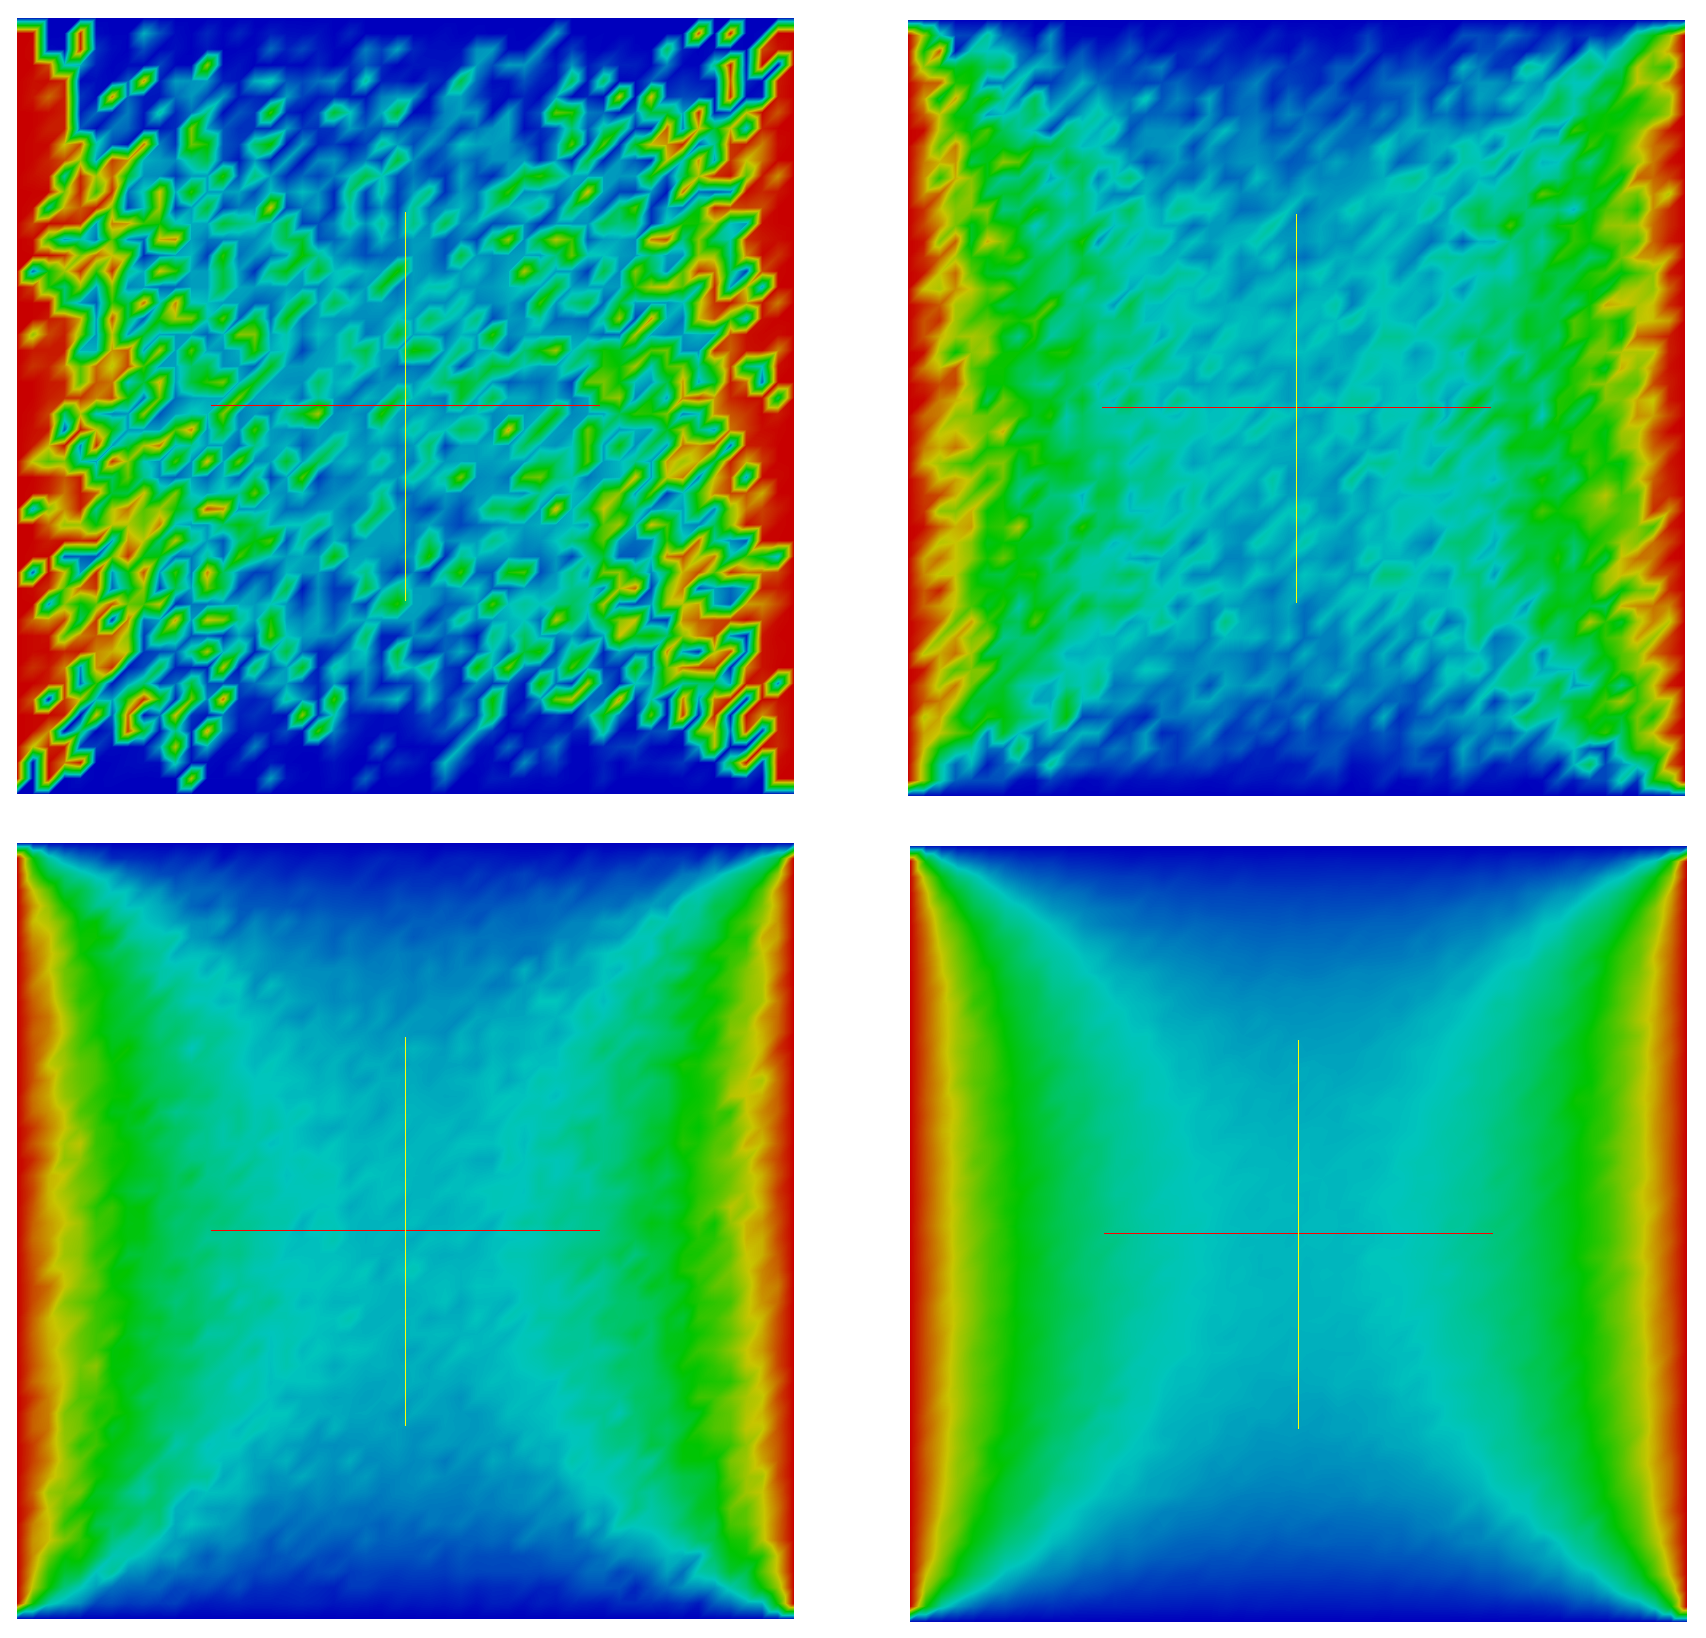
\includegraphics[width=6in]{chapters/mc_background/direct_evolution.png}
  \end{center}
  \caption{\textbf{Direct Monte Carlo solution to the heat equation
      with varying numbers of histories.} \textit{Top left: 1 history
      per state. Top right: 10 histories per state. Bottom left: 100
      histories per state. Bottom right: 1000 histories per state.}}
  \label{fig:direct_evolution}
\end{figure}
As the number of histories used per state is increased, the
statistical variance of the solutions is decreased as more tallies are
made. Starting with a single history at each state in the domain, the
high variance prevents a precise solution from being obtained although
we begin to see the solution take shape as expected. It is interesting
to note here that as the statistical uncertainty is reduced at each
grid point in the domain, the solution is resolved in a certain sense,
analogous to the convergence of a traditional iterative method.
\clearpage

\subsection{Adjoint Neumann-Ulam Method}
\label{sec:adjoint_mc}
An alternative to forward Monte Carlo matrix inversion is the adjoint
method. We begin by defining the linear system adjoint to
Eq~(\ref{eq:linear_problem}):
\begin{equation}
  \ve{A}^T \ve{y} = \ve{d}\:,
  \label{eq:adjoint_linear_problem}
\end{equation}
where $\ve{y}$ and $\ve{d}$ are the adjoint solution and source
vectors respectively and $\ve{A}^T$ is the adjoint operator for
$\ve{A} \in \mathbb{R}^{N \times N}$. We can split this equation to
mirror Eq~(\ref{eq:richardson_split}):
\begin{equation}
  \ve{y} = \ve{H}^T \ve{y} + \ve{d}\:.
  \label{eq:adjoint_split_system}
\end{equation}
As was required for convergence with the direct method using
Eq~(\ref{eq:richardson_split}), the spectral radius of $\ve{H}$ must
remain less than 1 as $\ve{H}^T$ contains the same eigenvalues and
therefore has the same spectral radius. By defining the following
adjoint inner product equivalence \cite{spanier_monte_1969}:
\begin{equation}
  \langle \ve{A}^T \ve{y}, \ve{x} \rangle = \langle \ve{y}, \ve{A}
  \ve{x} \rangle\:.
  \label{eq:adjoint_operator_product}
\end{equation}
it follows that:
\begin{equation}
  \langle \ve{x}, \ve{d} \rangle = \langle \ve{y}, \ve{b} \rangle\:.
  \label{eq:adjoint_vector_relation}
\end{equation}
Using these definitions, we can derive an estimator from the adjoint
method that will also give the solution vector, $\ve{x}$. As with the
direct method, we can acquire the adjoint solution by forming the
Neumann series by writing Eq~(\ref{eq:adjoint_split_system}) as:
\begin{equation}
  \ve{y} = (\ve{I} - \ve{H}^T)^{-1} \ve{d}\:,
  \label{eq:adjoint_split_system_2}
\end{equation}
which in turn yields the Neumann series using the adjoint operator:
\begin{equation}
  \ve{y} = \sum_{k=0}^{\infty} (\ve{H}^T)^k\ve{d}\:.
  \label{eq:adjoint_neumann_series}
\end{equation}
We expand this summation to again yield a series of transitions that
can be approximated by a Monte Carlo random walk sequence, this time
forming the Neumann series in reverse order:
\begin{equation}
  y_i = \sum_{k=0}^{\infty}\sum_{i_1}^{N}\sum_{i_2}^{N}\ldots
  \sum_{i_k}^{N}h_{i_k,i_{k-1}}\ldots h_{i_2,i_1} h_{i_1,i} d_{i_k}\:.
  \label{eq:adjoint_neumann_solution}
\end{equation}
We can readily build an estimator for the adjoint solution from this
series expansion, but we instead desire the solution to
Eq~(\ref{eq:linear_problem}). Here we have 2 unknowns, $\ve{y}$ and
$\ve{d}$, and therefore we require two constraints to close the
system. We use Eq~(\ref{eq:adjoint_vector_relation}) as the first
constraint and as a second constraint we select:
\begin{equation}
  \ve{d} = \boldsymbol{\delta}_j\:,
  \label{eq:adjoint_second_constraint}
\end{equation}
where $\boldsymbol{\delta}_j$ is one of a set of vectors in which the
$j^{th}$ component is the Kronecker delta function $\delta_{i,j}$. If
we apply Eq~(\ref{eq:adjoint_second_constraint}) to our first
constraint Eq~(\ref{eq:adjoint_vector_relation}), we get the following
convenient outcome:
\begin{equation}
  \langle \ve{y}, \ve{b} \rangle = \langle \ve{x},
  \boldsymbol{\delta}_j \rangle = x_j \:,
  \label{eq:inner_product_constraint}
\end{equation}
meaning that if we compute the inner product of the original source
and the adjoint solution using a delta function source, we recover one
component of the original solution.

In terms of radiation transport, this adjoint method is equivalent to
a traditional forward method where the initial state $i_0$ of the
random walk is determined by sampling the source vector $\ve{b}$ with
probabilities:
\begin{equation}
  P_{(i_0=i)}(\nu) = \frac{|b_i|}{||\ve{b}||_1}\:,
  \label{eq:adjoint_source_probability}
\end{equation}
with a random walk starting weight of:
\begin{equation}
  W_0 = ||\ve{b}||_1 \frac{b_i}{|b_i|}\:,
  \label{eq:adjoint_starting_weight}
\end{equation}
which gives the additional useful relation:
\begin{equation}
  b_{i_0} = W_0 P_{(i_0=i)}\:.
  \label{eq:adjoint_source_definition}
\end{equation}
As a result of using the adjoint system, we modify our probabilities
and weights using the \textit{adjoint Neumann-Ulam decomposition} of
$\ve{H}$:
\begin{equation}
  \ve{H}^{T} = \ve{P} \circ \ve{W}\:,
  \label{eq:adjoint_neumann_ulam}
\end{equation}
where now we are forming the decomposition with respect to the
transpose of $\ve{H}$. We then follow the same procedure as the direct
method for forming the probability and weight matrices in the
decomposition. Using the adjoint form, probabilities should instead be
column-scaled:
\begin{equation}
  p_{ij} = \frac{|h_{ji}|}{\sum_j |h_{ji}|}\:,
  \label{eq:adjoint_probability}
\end{equation}
such that we expect to select a new state, $j$, from the current state
in the random walk, $i$, by sampling column-wise (or row-wise if an
adjoint probability matrix is formed). Per
Eq~(\ref{eq:adjoint_neumann_ulam}), the transition weight is then
defined as:
\begin{equation}
  w_{ij} = \frac{h_{ji}}{p_{ij}}\:.
  \label{eq:adjoint_weight}
\end{equation}
Using the decomposition we can then define an expectation value for
the adjoint method. Given Eq~(\ref{eq:direct_permutation_weight}) as
the weight generated for a particular random walk permutation as in
Eq~(\ref{eq:mc_walk_permutation}) and our result from
Eq~(\ref{eq:inner_product_constraint}) generated by applying the
adjoint constraints, the contribution to the solution in state $j$
from a particular random walk permutation of $k$ events is then the
\textit{collision estimator}\footnote{The variance for this estimator
  is discussed in Appendix~\ref{chap:estimator_variance}.}:
\begin{equation}
  X_{j}(\nu) = \sum_{m=0}^k W_{m} \delta_{i_m,j}\:,
  \label{eq:adjoint_permutation_contribution}
\end{equation}
where the Kronecker delta indicates that the tally contributes only in
the current state, $i_m$, of the random walk.  Note here that the
estimator in Eq~(\ref{eq:adjoint_permutation_contribution}) does not
have a dependency on the source state as in
Eq~(\ref{eq:direct_permutation_contribution}), providing a remedy for
the situation in the direct method where we must start a random walk
in each source state for every permutation if we want to compute a
solution estimate for that state. In the adjoint method, we instead
tally in all states and those of lesser importance will not be visited
as frequently by the random walk. Finally, the expectation value using
all permutations is:
\begin{equation}
  E\{X_j\} = \sum_{\nu} P_{\nu} X_{j}(\nu)\:
  \label{eq:adjoint_expectation_value}
\end{equation}
which, if expanded in the same way as the direct method and utilizing
Eq~(\ref{eq:adjoint_source_definition}) to insert the source term,
directly recovers the exact solution:
\begin{equation}
  \begin{split}
    E\{X_j\} &=\sum_{k=0}^{\infty}\sum_{i_1}^{N}\sum_{i_2}^{N}\ldots
    \sum_{i_k}^{N} b_{i_0} p_{i_0,i_1}p_{i_1,i_2}\ldots
    p_{i_{k-1},i_k} w_{i_0,i_1}w_{i_1,i_2}\ldots
    w_{i_{k-1},i_k} \delta_{i_k,j} \\ &= x_{j}\:,
  \end{split}
  \label{eq:adjoint_expectation_expansion}
\end{equation}
therefore, also providing an unbiased Monte Carlo estimate of the
solution. It should be noted here that
Eq~(\ref{eq:adjoint_expectation_expansion}) only computes a single
component of our desired solution vector when really what we desire is
the entire solution vector. In an adjoint Monte Carlo simulation using
this estimator, the $w_{ij}$ elements that are added into the tally
for each state are only selected if/when the random walk currently
resides in that state. Much like a mesh tally in a particle transport
simulation, we have $N$ simultaneous tallies for $\ve{A} \in
\mathbb{R}^{N \times N}$ that will yield the entire solution vector.

Like the direct method, we also desire a criteria for random walk
termination for problems where only an approximate solution is
necessary. For the adjoint method, we utilize a \textit{relative
  weight cutoff}:
\begin{equation}
  W_f = W_c W_0\:,
  \label{eq:relative_weight_cutoff}
\end{equation}
where $W_c$ is defined as in the direct method. The adjoint random
walk will then be terminated after $m$ steps if $W_m < W_f$ as tally
contributions become increasingly small.

\subsubsection{Expected Value Estimator}
\label{subsec:expected_value_estimator}
In addition to the collision estimator, an additional estimator is
available due to the work of Okten \cite{okten_solving_2005} that uses
the method of expected values as a means to improve the Monte Carlo
estimate. As outlined by Spanier and Gelbard
\cite{spanier_monte_1969}, the method of expected values is a
deterministic averaging of events that may potentially occur in the
Monte Carlo random walk sequence. Okten applied this principle
directly to discrete Monte Carlo by forming the \textit{expected value
  estimator}\footnote{The variance for this estimator is discussed in
  Appendix~\ref{chap:estimator_variance}.} for a random walk of $k$
events:
\begin{equation}
  X_{j}(\nu) = b_j + \sum_{m=0}^k W_m h_{j,i_m}\,
  \label{eq:expected_value_estimator}
\end{equation}
where now the contribution of the iteration matrix is
deterministically averaged at step $m$ over all potential states $j$
that may be reached from the current state $i_m$. Via Okten, the
estimator can be shown to be unbiased through a comparison to the
collision estimator. We can first rewrite the summation in
Eq~(\ref{eq:expected_value_estimator}):
\begin{equation}
  X_{j}(\nu) = b_j + \sum_{m=0}^k \sum_{i=1}^N W_m
  \delta_{i_m,i} h_{ji}\,
  \label{eq:unbiased_eval_1}
\end{equation}
where $N$ is the number of states in the system. Immediately, we see
the collision estimator as defined by
Eq~(\ref{eq:adjoint_permutation_contribution}) and can therefore write
the expectation value as:
\begin{equation}
  E\{X_{j}\} = b_j + \sum_{i=1}^N E\{X_{i}\} h_{ji}\,
  \label{eq:unbiased_eval_2}
\end{equation}
which is equivalently is the $j^{th}$ component of
Eq~(\ref{eq:richardson_split}):
\begin{equation}
  E\{X_{j}\} = b_j + \sum_{i=1}^N x_{i} h_{ji}\,
  \label{eq:unbiased_eval_2}
\end{equation}
and is therefore an unbiased estimate. Compared to the collision
estimator, the expected value estimator provides additional
information at every step of the random walk, yielding potentially
better statistics with the same amount of transport
work. Conveniently, even if no Monte Carlo histories are computed, the
expected value estimator still deterministically computes the first
term of the Neumann Series, $\ve{H}^0\ve{b}$, whereas the collision
estimator will provide no information.

\subsubsection{Adjoint Method: Evolution of a Solution}
\label{subsec:adjoint_evolution}
As a means of visually demonstrating the adjoint Monte Carlo method,
again consider the 2-dimensional thermal diffusion problem with
sources on the left and right hand sides of the domain and a smaller
uniform source as shown in Figure~\ref{fig:heat_setup}. Using the
adjoint method with the collision estimator, the number of histories
sampled from the source was increased from 10 to 10,000,000 in order
to show its effects on the solution and the statistical nature of the
method. Figure~\ref{fig:adjoint_evolution} gives these results.
\begin{figure}[t!]
  \begin{center}
    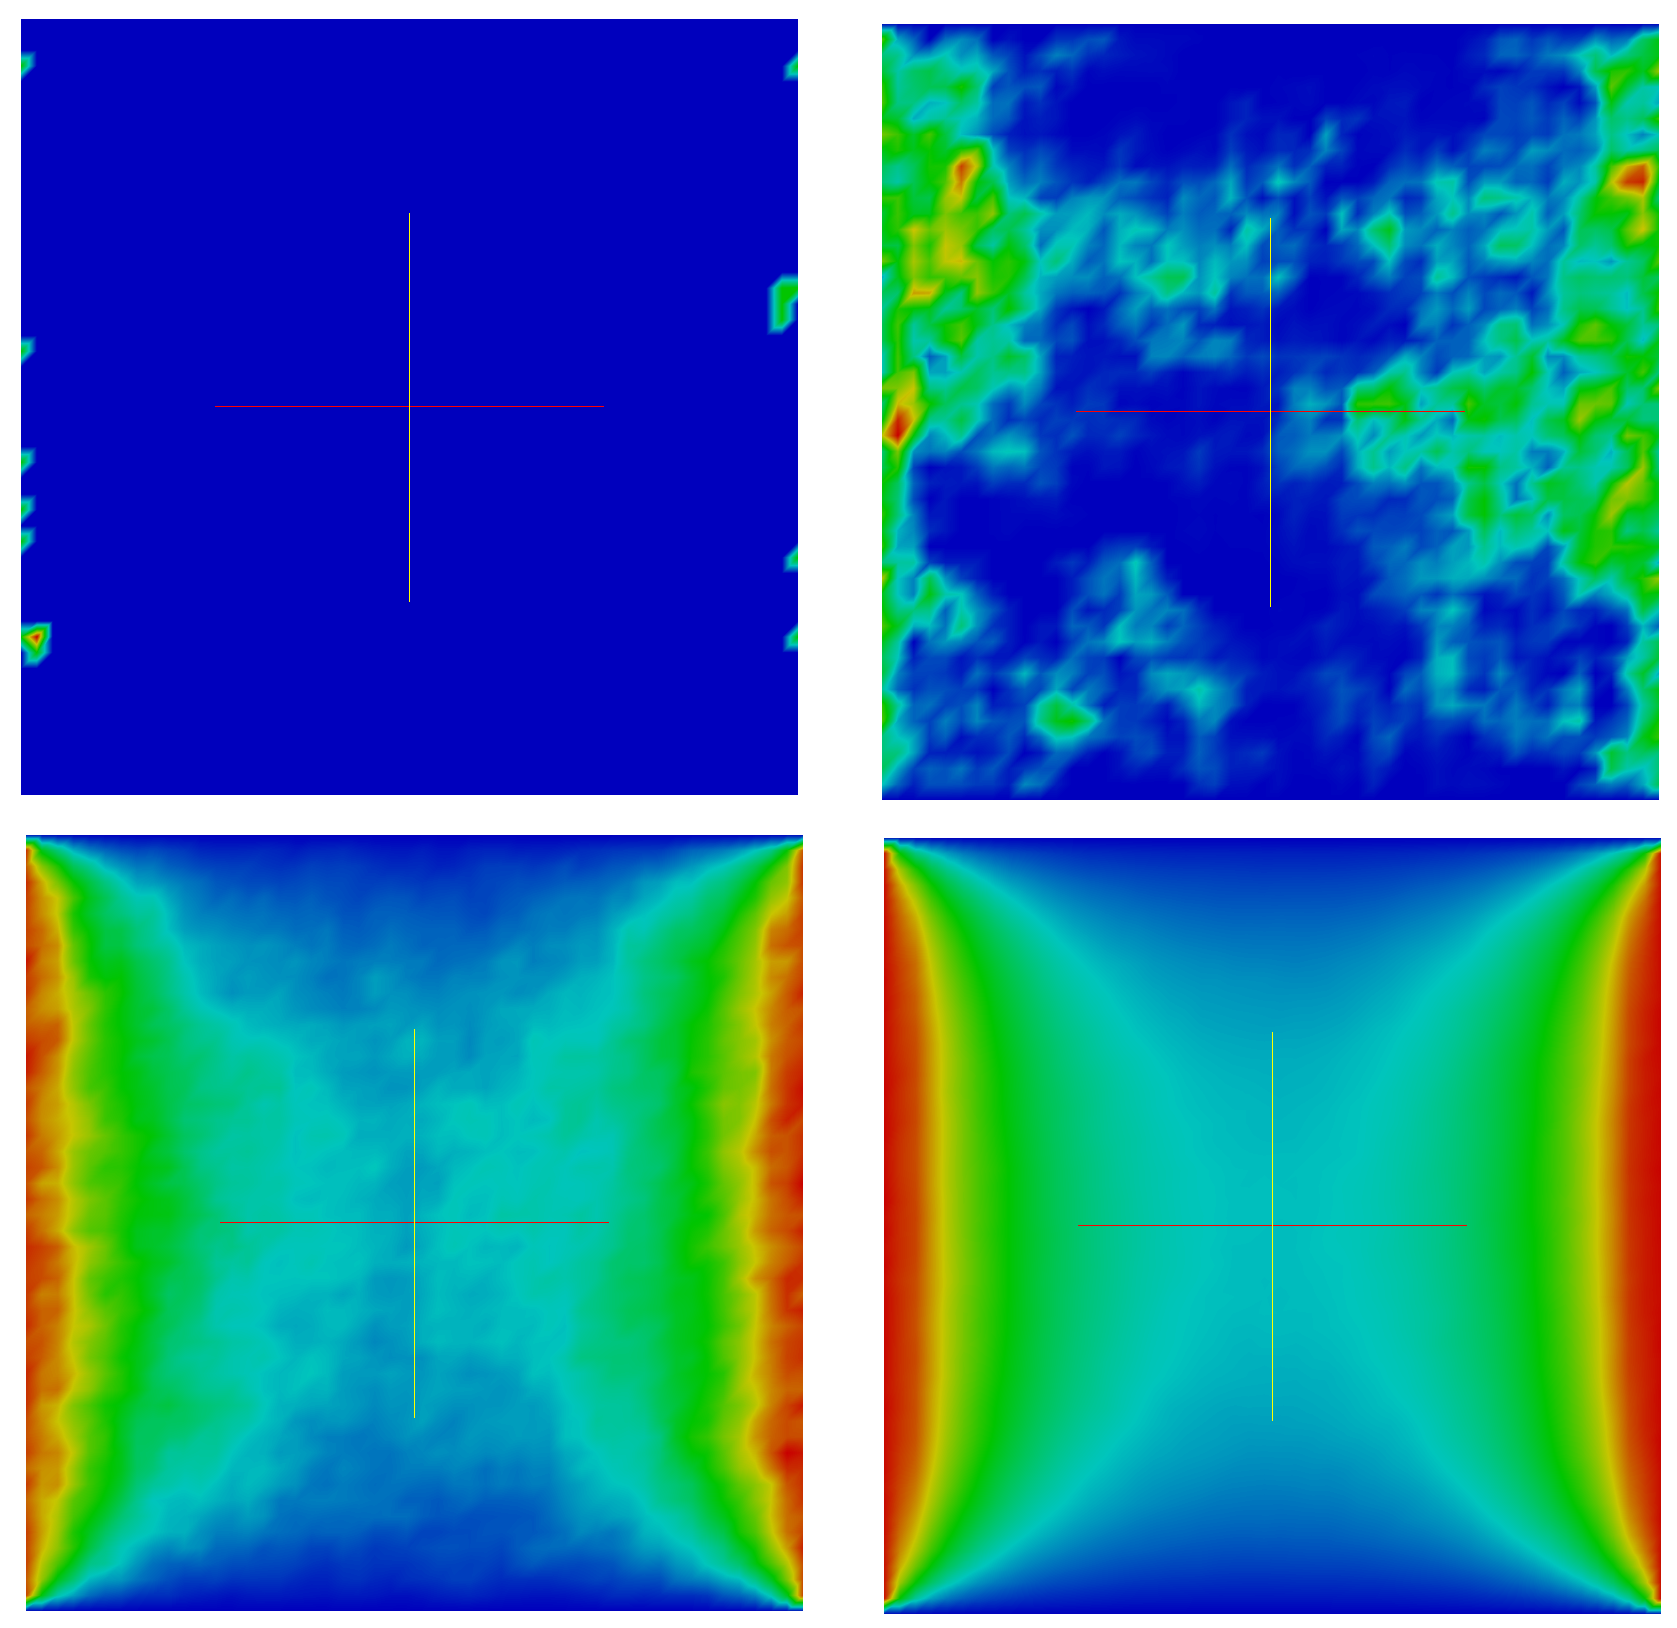
\includegraphics[width=6in]{chapters/mc_background/adjoint_evolution.png}
  \end{center}
  \caption{\textbf{Adjoint Monte Carlo solution to the heat equation
      with varying numbers of histories.} \textit{Top left: 10
      histories per state. Top right: 1,000 histories per
      state. Bottom left: 100,000 histories per state. Bottom right:
      10,000,000 histories per state.}}
  \label{fig:adjoint_evolution}
\end{figure}
As the number of histories used per state (or DOF) is increased, the
statistical variance of the solutions is decreased as more tally
contributions are made. At 10,000,000 histories per state, enough
information has been tallied to generate a reasonable estimate for the
structure of the solution. The visual difference between
Figures~\ref{fig:direct_evolution} and \ref{fig:adjoint_evolution} is
precisely that determined by their mathematics. As the adjoint
solution evolves with the addition of histories, more histories
emanate from the boundary the smaller uniform source in the domain
with more penetrating from the boundary into the domain and making
contributions to the tallies in those states as they are transported.

\clearpage

%%---------------------------------------------------------------------------%%
\section{Sequential Monte Carlo}
\label{sec:sequential_mc}
The direct and adjoint Neumann-Ulam methods described are limited by a
convergence rate of $1/\sqrt{N}$ by the Central Limit Theorem where
$N$ is the number of random walk permutations. In 1962, Halton
presented a residual Monte Carlo method that moves towards exponential
convergence rates \cite{halton_sequential_1962} and further refined
his work some years later \cite{halton_sequential_1994} with
applications of his work by the transport community confirming
exponential convergence rates \cite{evans_residual_2003}. Halton's
method, sequential Monte Carlo, utilizes the adjoint Monte Carlo
solver as a means of directly reducing the elements residual
vector. He proposed the following iterative scheme as a solution to
Eq~(\ref{eq:linear_problem})\:
\begin{subequations}
  \begin{gather}
    \ve{r}^k = \ve{b} - \ve{A}\ve{x}^k\:,\\  
    \ve{A}\boldsymbol{\delta}^{k} = \ve{r}^{k}\:,\\
    \ve{x}^{k+1} = \ve{x}^k + \boldsymbol{\delta}^{k}\:,
  \end{gather}
  \label{eq:sequential_monte_carlo}
\end{subequations}
where the correction $\boldsymbol{\delta}^k$ is computed by the
adjoint Monte Carlo method at each iteration. The merits of Halton's
approach are immediately visible in that we have now broken the
binding of the convergence rate to the Central Limit Theorem. Here,
the Monte Carlo solver is used to produce a correction from the
residual, analogous to using the residual to extract a correction from
the search subspace in a projection method. By doing this, the Monte
Carlo error is bound in the correction used to update the solution and
therefore does not explicitly manifest itself in the overall
convergence of the solution. The downside of such a method is that if
the solution guess is poor, then many iterations are required in order
to reach exponential converge as the Monte Carlo error (and therefore
the Central Limit Theorem) does dominate in this situation.

%%---------------------------------------------------------------------------%%
\section{Monte Carlo Synthetic Acceleration}
\label{sec:mcsa}
Using the ideas of Halton, Evans and Mosher recently developed a Monte
Carlo solution method that was not prohibited severely by the quality
of the initial guess for the system \cite{evans_monte_2009} and later
applied it more rigorously as a solution mechanism for the radiation
diffusion equation \cite{evans_monte_2012}. Their approach was instead
to use residual Monte Carlo as a synthetic acceleration for a
stationary method. To derive this method, we begin by splitting the
operator in Eq~(\ref{eq:linear_problem})
\begin{equation}
  \ve{x} = (\ve{I} - \ve{A})\ve{x} + \ve{b}\:.
  \label{eq:linear_split}
\end{equation}
With this we can then define the stationary method
\textit{Richardson's iteration} as:
\begin{equation}
  \ve{x}^{k+1} = (\ve{I} - \ve{A})\ve{x}^k + \ve{b}\:,
  \label{eq:richardsons_iteration}
\end{equation}
which will converge if $\rho(\ve{I} - \ve{A}) < 1$. We then define the
solution error at the $k^{th}$ iterate relative to the true solution:
\begin{equation}
  \delta \ve{x}^k = \ve{x} - \ve{x}^k\:.
  \label{eq:mcsa_error}
\end{equation}
Subtracting Eq~(\ref{eq:richardsons_iteration}) from
Eq~(\ref{eq:linear_split}) we get:
\begin{equation}
  \delta \ve{x}^{k+1} = (\ve{I} - \ve{A})\delta \ve{x}^k\:.
  \label{eq:mcsa_setup_1}
\end{equation}
Subtracting from this $(\ve{I} - \ve{A})\delta \ve{x}^{k+1}$ yields:
\begin{equation}
  \begin{split}
    \ve{A}\delta \ve{x}^{k+1} &= (\ve{I} -
    \ve{A})(\ve{x}^{k+1}-\ve{x}^{k}) \\ &= \ve{r}^{k+1}\:.
    \label{eq:mcsa_setup_2}
  \end{split}
\end{equation}
Using this, we define the following scheme that will converge in one
iteration if $\ve{A}$ is inverted exactly:
\begin{subequations}
  \begin{gather}
    \ve{x}^{k+1} = (\ve{I} - \ve{A})\ve{x}^k + \ve{b}\:,\\
    \ve{A} \delta \ve{x}^{k+1} = \ve{r}^{k+1}\:,\\
    \ve{x} = \ve{x}^{k+1} + \delta \ve{x}^{k+1}\:.
  \end{gather}
  \label{eq:mcsa_setup_3}
\end{subequations}
However, $\ve{A}$ is only approximately inverted by our numerical
methods and therefore we instead pose an iterative scheme in which the
Monte Carlo solvers are used to invert the operator. The
\textit{Fixed-Point Monte Carlo Synthetic Acceleration} (MCSA) method
is defined as:
\begin{subequations}
  \begin{gather}
    \ve{x}^{k+1/2} = \ve{x}^k + \ve{r}^k\:,\\
    \ve{r}^{k+1/2} = \ve{b} - \ve{A}\ve{x}^{k+1/2}\:,\\
    \ve{A}\delta\ve{x}^{k+1/2} = \ve{r}^{k+1/2}\:,\\
    \ve{x}^{k+1} = \ve{x}^{k+1/2} + \delta \ve{x}^{k+1/2}\:,\\
    \ve{r}^{k+1} = \ve{b} - \ve{A}\ve{x}^{k+1}\:,
  \end{gather}
  \label{eq:mcsa}
\end{subequations}
where a Neumann-Ulam Monte Carlo method is used to generate the
solution correction from the residual and Richardson's iteration in
the first step has been rewritten as a residual correction. Using
Monte Carlo in this way achieves the same effect as Halton's method,
decoupling its convergence rate from the overall convergence rate of
the method. Here, the approximate Monte Carlo solution is not driven
to a particular convergence as it merely supplies a correction for the
initial guess generated by Richardson's iteration. Rather, only a set
number of histories are required using the Neumann-Ulam method to
generate the correction. In addition, the fact that the scheme in
Eq~(\ref{eq:mcsa_setup_3}) will converge in one iteration if $\ve{A}$
is inverted exactly means that as more and more stochastic histories
are used to compute the correction and the error is reduced towards
zero, the number of iterations required for MCSA to converge should
decrease accordingly, thus accelerating the solution.

In addition to the Monte Carlo solver parameters dictating the number
of histories and weight cutoff, the outer MCSA iterations also have
the following stopping criteria:
\begin{equation}
  ||\ve{r}||_\infty < \epsilon \ ||\ve{b}||_\infty\:,
  \label{eq:mcsa_stopping_criteria}
\end{equation}
where $\epsilon$ is a user-defined parameter. As with any iterative
method, other stopping criteria using other vector norms could be
computed, however, for this work we will only use
Eq~(\ref{eq:mcsa_stopping_criteria}). We therefore have 3 parameters
to tune in an MCSA implementation: the number of Monte Carlo histories
computed in the Neumann-Ulam solve during each MCSA iteration, the
weight cutoff for those histories, and the total MCSA convergence
tolerance as specified by $\epsilon$.

\subsection{Alternative Fixed Point Iterations}
\label{subsubsec:alternative_fixed_point}
In addition to the basic Richardson iteration, the MCSA algorithm
presented in Eq~(\ref{eq:mcsa}) can be used to accelerate any fixed
point iteration which only depends on the state (typically the
residual) of the last iteration. As outlined in
Appendix~\ref{ch:linear_problem}, subspace methods take on a general
form using the Petrov-Galerkin conditions as constraints for
extracting a correction from the search subspace as given by
Eq~(\ref{eq:linear_projection_iteration}). Those that are
one-dimensional may be used with fixed-point MCSA as they only depend
the previous iteration for information. As an example, for
positive-definite but not necessarily symmetric problems, the minimal
residual iteration \cite{saad_iterative_2003} can be used in
conjunction with MCSA where the residual vector, $\mathbf{r}$, defines
the search subspace and the action of the linear operator on the
residual vector, $\mathbf{A}\mathbf{r}$, defines the constraint
subspace. Using this, we can then define an MCSA scheme that
accelerates the minimal residual iteration:
\begin{subequations}
  \begin{gather}
    \alpha = \frac{\langle \mathbf{A}\mathbf{r}^k, \mathbf{r}^k
      \rangle}{\langle \mathbf{A}\mathbf{r}^k, \mathbf{A}\mathbf{r}^k
      \rangle}\:, \\
    \ve{x}^{k+1/2} = \ve{x}^k + \alpha \ve{r}^k\:,
    \label{eq:min_res_correction}\\
    \ve{r}^{k+1/2} = \ve{b} - \ve{A}\ve{x}^{k+1/2}\:,\\ 
    \ve{A}\delta\ve{x}^{k+1/2} = \ve{r}^{k+1/2}\:,\\ 
    \ve{x}^{k+1} = \ve{x}^{k+1/2} + \delta\ve{x}^{k+1/2}\:,\\ 
    \ve{r}^{k+1} = \ve{b} - \ve{A}\ve{x}^{k+1}\:.
  \end{gather}
  \label{eq:mcsa_min_res}
\end{subequations}
where $\alpha$ is an optimal extrapolation parameter generated from
the constraints. Interestingly, this scheme is nearly identical to the
Richardson iteration version in Eq~(\ref{eq:mcsa}) except now the
additional extrapolation parameter, $\alpha$, is applied to the
residual correction in Eq~(\ref{eq:min_res_correction}) as a means of
selecting a more optimal search direction at each iteration,
potentially further improving convergence.

\subsection{Preconditioning MCSA}
\label{subsec:stochastic_preconditioning}
In most cases, at least a minimal amount of \textit{preconditioning}
of the linear system will be required in order to use the class of
stochastic methods described. Although these methods have no symmetry
requirements for convergence, they do require that the spectral radius
of the iteration matrix be less than one. Preconditioning serves as a
means of achieving this by altering the eigenvalue spectrum of the
iteration matrix.

\subsubsection{Basic Preconditioning}
\label{subsubsec:basic_mcsa_preconditioning}
As an example of basic preconditioning, to achieve a spectral radius
of less than one for diagonally dominant matrices point Jacobi
preconditioning can be used such that the preconditioning matrix
$\ve{M}$ is:
\begin{equation}
  \ve{M} = diag(\ve{A})\:,
  \label{eq:jacobi_preconditioner}
\end{equation}
which may be trivially inverted. With the application of this
preconditioner we are instead solving the following scaled linear
system:
\begin{equation}
  \ve{M}^{-1}\ve{A}\ve{x} = \ve{M}^{-1}\ve{b}\:.
  \label{eq:jacobi_precond_linear_problem}
\end{equation}
Next, we can apply MCSA to solve
Eq~(\ref{eq:jacobi_precond_linear_problem}): 
\begin{subequations}
  \begin{gather}
    \ve{x}^{k+1/2} = \ve{x}^k +
    \ve{M}^{-1}\ve{r}^k\:,\\ \ve{r}^{k+1/2} =
    \ve{b}-\ve{A}\ve{x}^{k+1/2}\:,\\ \ve{M}^{-1}\ve{A}\delta\ve{x}^{k+1/2}
    = \ve{M}^{-1}\ve{r}^{k+1/2}\:,\\ \ve{x}^{k+1} = \ve{x}^{k+1/2} +
    \delta \ve{x}^{k+1/2}\:,\\
    \ve{r}^{k+1} = \ve{b} - \ve{A}\ve{x}^{k+1}\:,
    \label{eq:jacobi_preconditioned_mcsa}
  \end{gather}
\end{subequations}
where the Neumann-Ulam Monte Carlo solve now has a preconditioned
operator from which to build weights and probabilities for transport
and a preconditioned source vector to sample.

Choosing point Jacobi preconditioning with MCSA is advantageous for
several reasons. First, $\rho(\ve{I} - \ve{M}^{-1}\ve{A}) < 1$ is true
for all $\ve{A}$ that is diagonally dominant and is easy to formulate
because the inversion of $\ve{M}$ is trivial. Second, because the
Monte Carlo method used within MCSA to compute the correction operates
on a linear problem with the preconditioned operator, then $\ve{H}$ in
the Neumann-Ulam solver will have a zero term in each of its diagonal
elements, thereby eliminating all in-state transitions during the
random walk sequence. Because of this, point Jacobi preconditioning
should be considered for many classes of problems, regardless of any
other preconditioning that is applied to the system. In addition,
Jacobi preconditioning has been shown to be an effective
preconditioning mechanism for MCSA when used with the thermal
radiation diffusion equation \cite{evans_monte_2012}.

\clearpage

\subsubsection{General Preconditioning Strategies}
\label{subsubsec:general_mcsa_preconditioning}
It is possible to use general left, right, and left/right
preconditioning with MCSA by carefully considering the underlying
Monte Carlo problem that will be solved with the Neumann-Ulam
method. We consider here the general left/right preconditioned method
as the left or right preconditioned methods can be inferred from its
formulation. We consider a left preconditioner $\ve{M_L}$ and a right
preconditioner $\ve{M_R}$. The left/right preconditioned linear
problem is then:
\begin{equation}
  \ve{M}_L^{-1}\ve{A}\ve{M}_R^{-1}\ve{M}_R\ve{x} = \ve{M}_L^{-1}\ve{b}\:.
  \label{eq:left_right_linear_problem}
\end{equation}
To handle the right preconditioning, the system is written with a
substitution of variables:
\begin{equation}
  \ve{M}_L^{-1}\ve{A}\ve{M}_R^{-1}\ve{u} = \ve{M}_L^{-1}\ve{b}\:,
  \label{eq:left_right_subs_problem}
\end{equation}
with
\begin{equation}
  \ve{x} = \ve{M}_R^{-1}\ve{u}\:.
  \label{eq:left_right_recover}
\end{equation}
To apply such a method to MCSA, we solve for the substituted variable
$\ve{u}$ during the iteration sequence:
\begin{subequations}
  \begin{gather}
    \ve{u}^{k+1/2} = \ve{u}^k + \ve{r}^k\:,\\
    \ve{r}^{k+1/2} = \ve{M}_L^{-1}(\ve{b}-\ve{A}\ve{M}_R^{-1}\ve{u}^{k+1/2})\:,\\ 
    \ve{M}_L^{-1}\ve{A}\ve{M}_R^{-1}\delta\ve{u}^{k+1/2} = \ve{r}^{k+1/2}\:,\\ 
    \ve{u}^{k+1} = \ve{u}^{k+1/2} + \delta \ve{u}^{k+1/2}\:,\\
    \ve{r}^{k+1} = \ve{M}_L^{-1}(\ve{b}-\ve{A}\ve{M}_R^{-1}\ve{u}^{k+1})\:,
  \end{gather}
  \label{eq:left_right_mcsa}
\end{subequations}
and then recover the original solution vector with
Eq~(\ref{eq:left_right_recover}) after convergence. For the Monte
Carlo problem, we isolate the generation of the correction:
\begin{equation}
  \ve{M}_L^{-1}\ve{A}\ve{M}_R^{-1}\delta\ve{u}^{k+1/2} = \ve{r}^{k+1/2}\:,
  \label{eq:left_right_correction}
\end{equation}
and note that the preconditioned residual of the substituted variable
is now serving as the source and the new iteration matrix is:
\begin{equation}
  \ve{H} = \ve{I} - \ve{M}_L^{-1}\ve{A}\ve{M}_R^{-1}\:.
  \label{eq:left_right_iteration_matrix}
\end{equation}
As we require $(i,j)$ element-wise access to the iteration matrix in
order to construct probabilities and weights for the Monte Carlo
procedure from the Neumann-Ulam decomposition, the \textit{composite
  operator}, $\ve{M}_L^{-1}\ve{A}\ve{M}_R^{-1}$, must be formed via
matrix-matrix multiplication. 

Several possible shortcomings of this preconditioning approach are
readily observed. First, the matrix-matrix multiplication operation
for sparse, parallel distributed matrices is significantly more
expensive than a matrix-vector multiplication operation. Second, each
preconditioner must be explicitly inverted, an operation in itself
that may be expensive and which prohibits the use of any
preconditioners which provide no mechanism to extract their
inverse. Third, for many modern preconditioning methods, this
inversion may yield dense matrices, destroying sparsity and further
impeding the performance of a matrix-matrix multiplication
operation. It is also interesting to note that the Monte Carlo problem
in the general left/right preconditioned scheme given by
Eq~(\ref{eq:left_right_correction}) is not fully left/right
preconditioned (meaning that we do not recover $\ve{x}$), but instead
part of a sequence for finding the substituted variable $\ve{u}$. We
do, however, gain the benefits of this general preconditioning by
building the iteration matrix in
Eq~(\ref{eq:left_right_iteration_matrix}) from the fully
preconditioned linear operator. In addition, for MCSA to apply to
increasingly difficult problems, more advanced preconditioning
techniques that require the generation of the composite operator may
be necessary for convergence.

%%---------------------------------------------------------------------------%%
\section{Monte Carlo Synthetic Acceleration Analysis}
\label{sec:mcsa_analysis}
In this section we analyze the effects of various MCSA parameters to
better our understanding of the algorithm and facilitate future
work. In addition, we demonstrate the effectiveness of MCSA as
compared to Halton's Sequential Monte Carlo method. To do this, we
choose the two-dimensional time-dependent Poisson equation as a simple
model transport problem\footnote{The Poisson equation is a simple form
  of the diffusion equation and has a similar elliptic character in
  its time-dependent form to the neutron transport equations that will
  be solved in the next chapter.}:
\begin{equation}
  \frac{\partial \ve{u}}{\partial t} = \nabla^2 \ve{u}\:.
  \label{eq:poisson_equation}
\end{equation}
For all comparisons, a single time step is computed with backwards Euler time
integration. The Laplacian is differenced on a square Cartesian grid with a
second-order five-point stencil,
\begin{equation}
  \nabla^2_5 = \frac{1}{\Delta^2}[u_{i-1,j} + u_{i+1,j} + u_{i,j-1} +
    u_{i,j+1} - 4 u_{i,j}]\:,
  \label{eq:five_point_stencil}
\end{equation}
and a fourth-order nine-point stencil,
\begin{multline}
  \nabla^2_9 = \frac{1}{6\Delta^2}[4 u_{i-1,j} + 4 u_{i+1,j} + 4
    u_{i,j-1} + 4 u_{i,j+1} + u_{i-1,j-1}\\ + u_{i-1,j+1} +
    u_{i+1,j-1} + u_{i+1,j+1} - 20 u_{i,j}]\:,
  \label{eq:nine_point_stencil}
\end{multline}
both assuming a grid size of $\Delta$ in both the $i$ and $j$ directions. For
a single time step solution, we then have the following sparse linear system
to be solved with the MCSA method:
\begin{equation}
  \ve{A} \ve{u}^{n+1} = \ve{u}^n\:.
  \label{eq:poisson_eq_lin_sys}
\end{equation}
Both the stencils will be used to vary the size and density of the sparse
linear system in Eq.~(\ref{eq:poisson_eq_lin_sys}).

\subsection{Monte Carlo Method Selection}
\label{sec:mc_method_selection}
The MCSA method defined in Eq.~(\ref{eq:mcsa}) uses the adjoint method
to estimate the error in a residual Monte Carlo solve instead of the
direct method outlined in \S\ref{sec:direct_mc}. To demonstrate the
effectiveness of the adjoint method over the direct method within the
context of MCSA, we solve Poisson equation in a series of numerical
experiments. A timing and convergence study is used to demonstrate
the effectiveness of the adjoint method with the collision estimator
as compared to the direct method. To assess both the CPU time and
number of iterations required to converge to a solution, a problem of
constant $\Delta$ was used with varying values of the number of mesh
elements, fixing the spectral radius of the system at a constant value
for each variation. Both the five-point and nine-point stencils were
used with both the direct and adjoint solvers. For each case, $N
\times N$ total random walk permutations were computed per MCSA
iteration where $N \times N$ is the number of discrete grid points (or
degrees of freedom) in the system. Solver parameters were set to a
weight cutoff of \sn{1}{-4} for the stochastic linear solver and a
convergence tolerance of \sn{1}{-8} for the MCSA iterative solver.
Figure~\ref{fig:poisson_cpu_time} gives the CPU time needed for each
case to converge in seconds, and Figure~\ref{fig:poisson_iterations}
gives the number of iterations needed for each case to converge to the
specified tolerance, both as a function of the problem size. All
computations presented in this section and the remaining sections of
this chapter were completed on a 3.0 GHz Intel Core 2 Quad Q9650 CPU
machine with 16 GB 1067 MHz DDR3 memory.

\begin{figure}[t!]
  \centering
  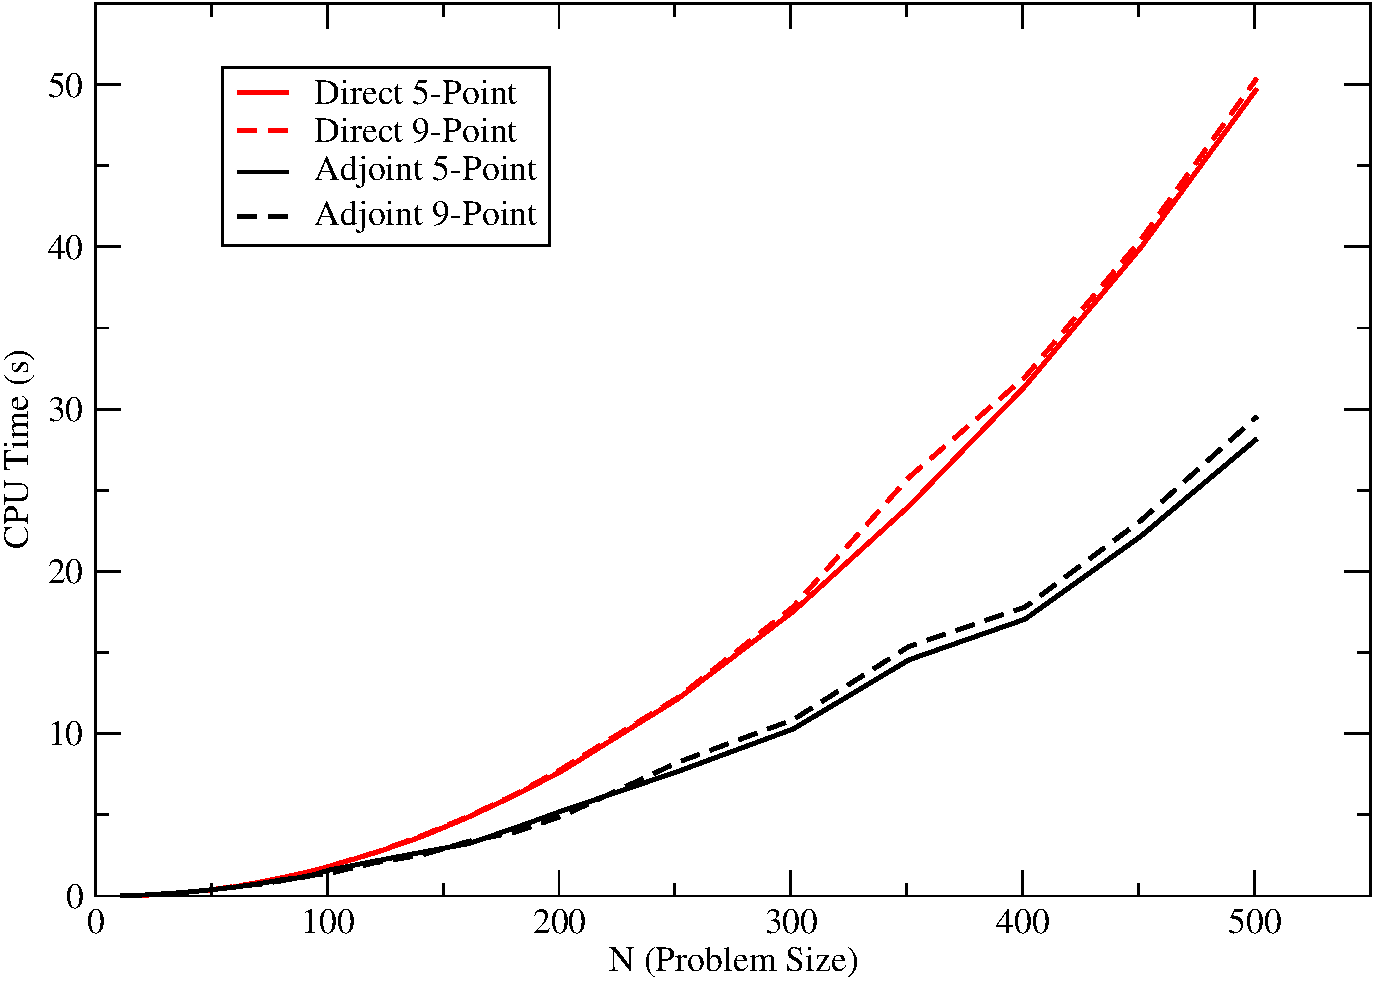
\includegraphics[width=5in,clip]{chapters/mc_background/dir_adj_cpu.pdf}
  \caption{\textbf{CPU Time (s) to converge vs. Problem Size ($N$ for
      an $N \times N$ square mesh).} \textit{Both the adjoint and
      direct solvers are used with the five point and nine point
      stencils. A CPU time speedup is noted with the adjoint method
      due to the higher density of random walk events in regions with
      a large residual.}}
  \label{fig:poisson_cpu_time}
\end{figure}

\begin{figure}[t!]
  \centering
  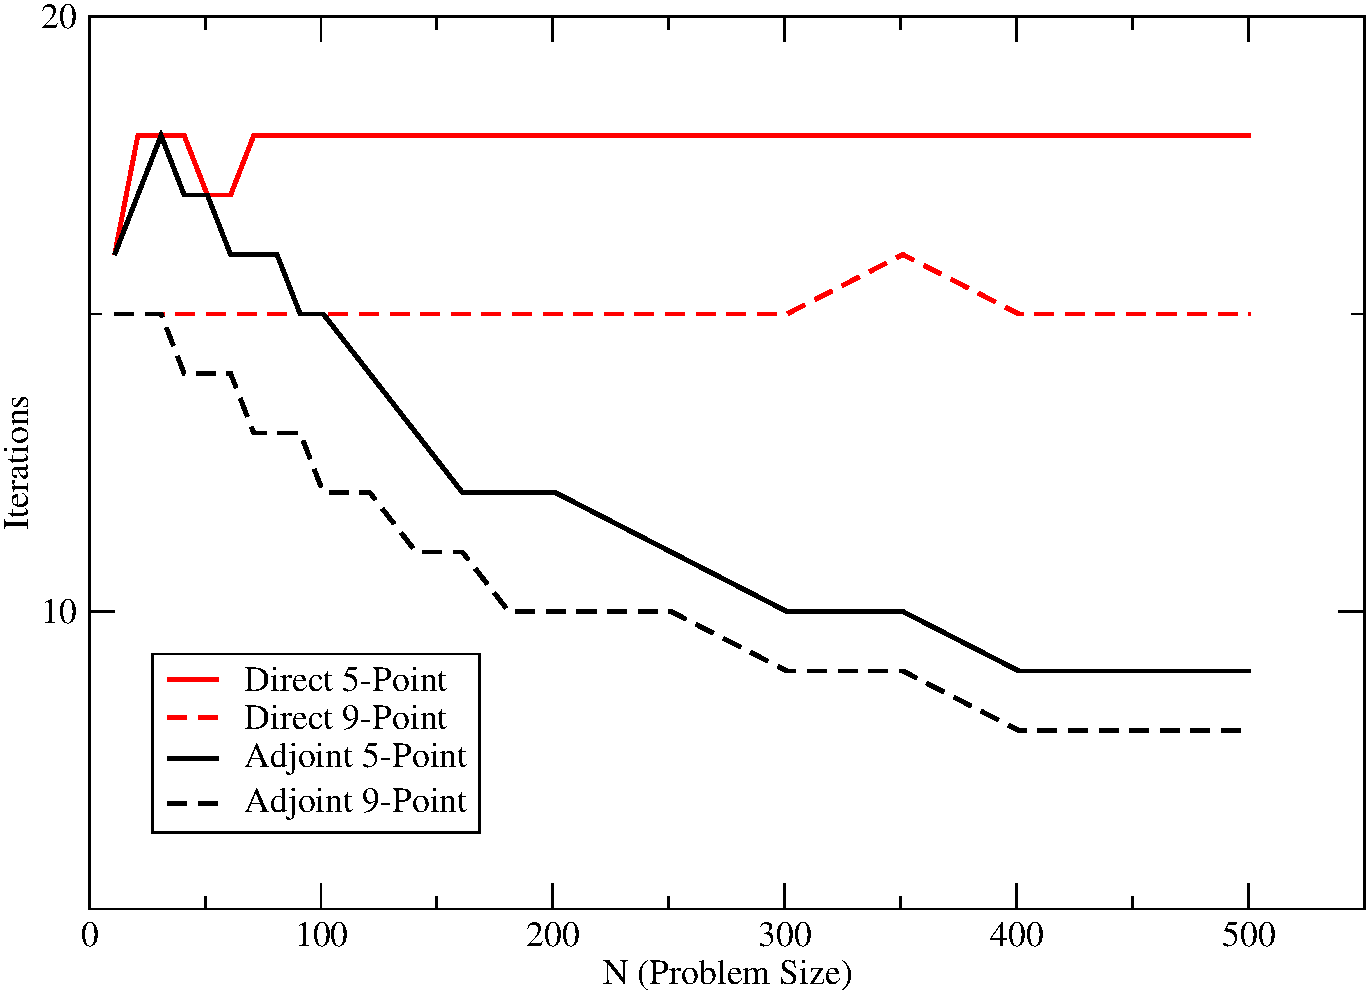
\includegraphics[width=5in,clip]{chapters/mc_background/dir_adj_iterations.pdf}
  \caption{\textbf{Iterations to converge vs. Problem Size ($N$ for an
      $N \times N$ square mesh).} \textit{Both the adjoint and direct
      solvers are used with the five-point and nine-point stencils.}}
  \label{fig:poisson_iterations}
\end{figure}

We see clearly in Figure~\ref{fig:poisson_cpu_time} that the using the
adjoint solver with MCSA results in a speedup over the direct solver
while the number of iterations required to converge is also reduced as
shown in Figure~\ref{fig:poisson_iterations}. We expect this for
several reasons. First, with an equivalent number of histories
specified for both solvers per MCSA iteration and a system of size $N
\times N$, the direct solver will compute a single random walk for
each state in the system per iteration to acquire a solution in that
state. This is necessary in the direct method to ensure a contribution
from each state as the random walk sequence will only contribute to
the starting state. For the adjoint method, a total of $N \times N$
random walk events will have their starting state determined by
sampling the residual vector. Because the random walk sequence
contributes to the state in which it currently resides, sampling the
residual vector as the Monte Carlo source gives a higher density of
random walk events in regions with a high residual, thus giving a more
accurate correction in that region due to reduced statistical
error. 

From an iteration perspective, Figure~\ref{fig:poisson_iterations}
shows that using the direct method yields a roughly unchanging number
of iterations required to converge as the problem size
increases. Again, if we desire a correction value for all states in
the problem, then we must start a random walk in each state in the
system without taking into account the structure of the residual
vector. Because of this, as the problem size grows adding histories is
ineffective as many are added in states where the error is smaller
than in other parts of the problem, ultimately not reducing the number
of iterations needed to converge. Conversely, as the problem size
grows in the adjoint method, the additional stochastic histories that
will be computed are concentrated in regions with a large residual,
further reducing the stochastic error in the correction in those
regions and subsequently reducing the required number of iterations to
converge.

As an additional comparison, the convergence behavior of MCSA can be
analyzed using both the adjoint and direct solvers to detect any
performance benefits. To assess the convergence properties of MCSA
using each solver and stencil, the infinity norm of the residual
computed in Eq.~(\ref{eq:mcsa}) was collected at each iteration for a
fixed problem size of $N=500$. Figure~\ref{fig:poisson_convergence}
gives the results of these computations. We note that using the
adjoint method with the same number of stochastic histories per MCSA
iteration gives a faster rate of converge for the same reasons as
above. We also note here that fewer iterations are required for
convergence when the 9-point stencil is used to discretize the
Laplacian operator (although at no gain in speed as given by the
results in Figure~\ref{fig:poisson_cpu_time}). This is due to the fact
that the smaller discretization error directly corresponds to a more
well defined residual source generated by the Richardson extrapolation
for the Monte Carlo calculation. In addition, the better defined
source is transported through a domain described more accurately by
the 9-point stencil, thus yielding a more accurate correction vector
from the Monte Carlo calculation.

\begin{figure}[t!]
  \centering
  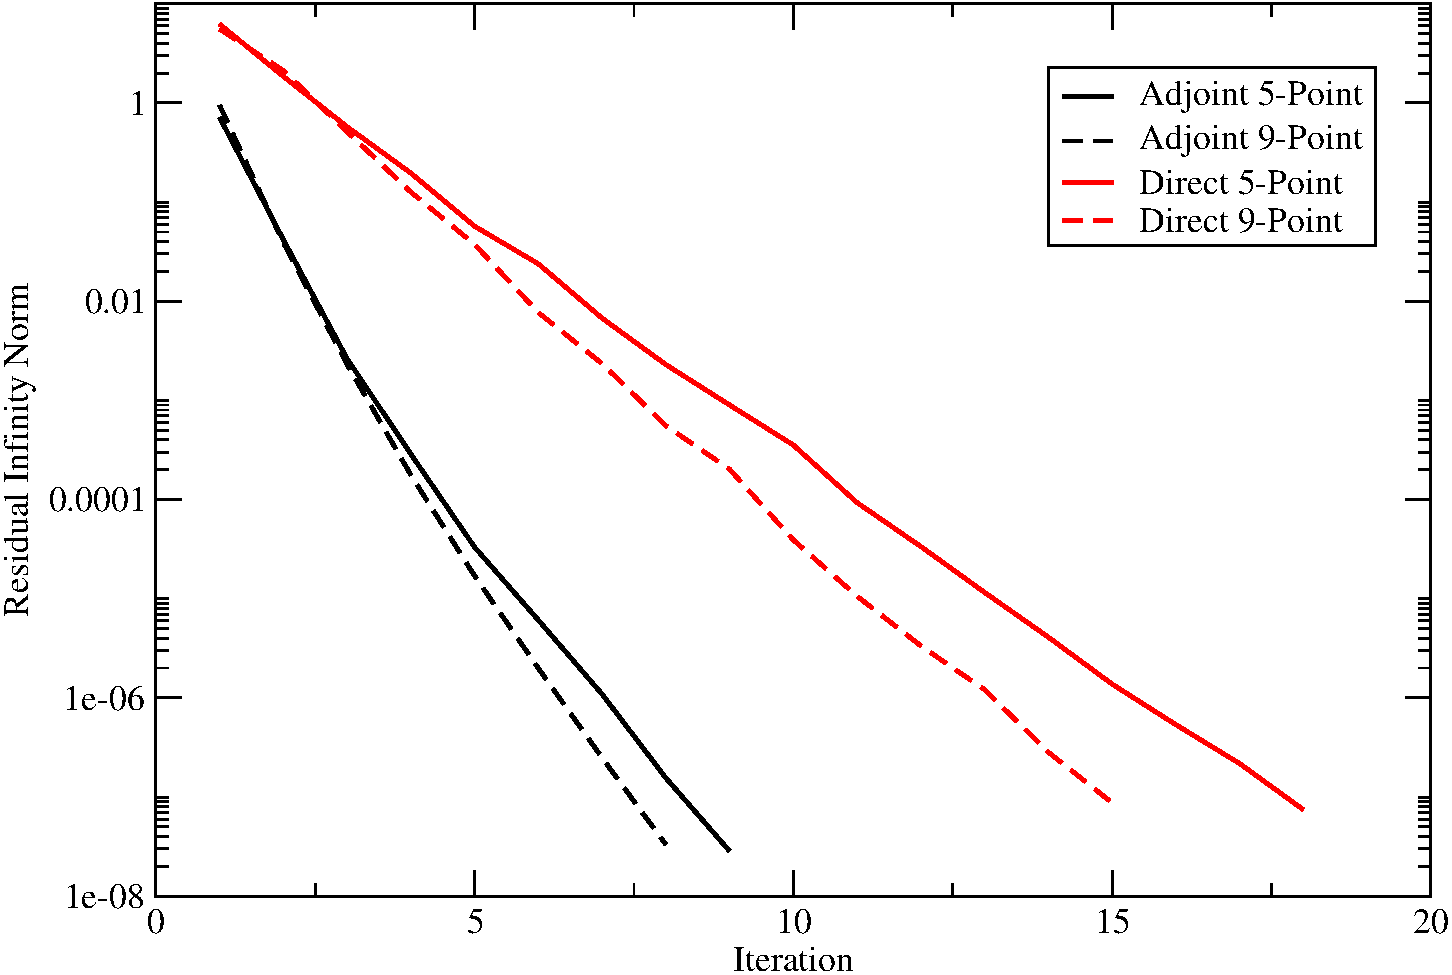
\includegraphics[width=5in,clip]{chapters/mc_background/dir_adj_conv.pdf}
  \caption{\textbf{Infinity norm of the solution residual
      vs. iteration number for a problem of size $N=500$.}
    \textit{Both the adjoint and direct solvers are used with the five
      point and nine point stencils. A higher rate of convergence is
      observed for MCSA using the adjoint Monte Carlo solver as
      compared to the direct method when both solvers compute the same
      number of random walks per iteration.}}
  \label{fig:poisson_convergence}
\end{figure}

\subsection{MCSA Comparison to Sequential Monte Carlo}
\label{subsec:sequential_comparison}
To further motivate using Monte Carlo Synthetic Acceleration, we
compare its performance to Halton's Sequential Monte Carlo. For this
comparison, we use the same transient Poisson problem as described in
the previous section and choose only the 5-point stencil to discretize
the Laplacian operator as the previous results yielded little
qualitative difference between the discretizations. Both MCSA and
Halton's method are used with the adjoint Monte Carlo solver and the
collision estimator. In order to complete the same study as in the
previous section, the number of histories computed by the Monte Carlo
solver at each iteration had to be doubled to $2 \times N \times N$ in
order to ensure convergence in Sequential Monte Carlo Method. For the
majority of the problems in the previous section, the Sequential
method used with $N \times N$ histories would not converge.

Figure~\ref{fig:seq_cpu_time} gives the CPU time results for this
comparison as a function of problem size while
Figure~\ref{fig:seq_iterations} gives the number of iterations to
converge as a function of problem size with a convergence tolerance of
\sn{1}{-8}. In both cases, using the Monte Carlo solver as a synthetic
acceleration rather than in a pure residual Monte Carlo scheme
resulted in a reduction in both CPU time and iterations required to
converge. The additional Richardson extrapolation between each Monte
Carlo solve in the MCSA method gives a better converged residual
source to use with the Monte Carlo calculation while the Sequential
method requires more iterations to achieve the same level of
convergence in the residual.

\begin{figure}[t!]
  \centering
  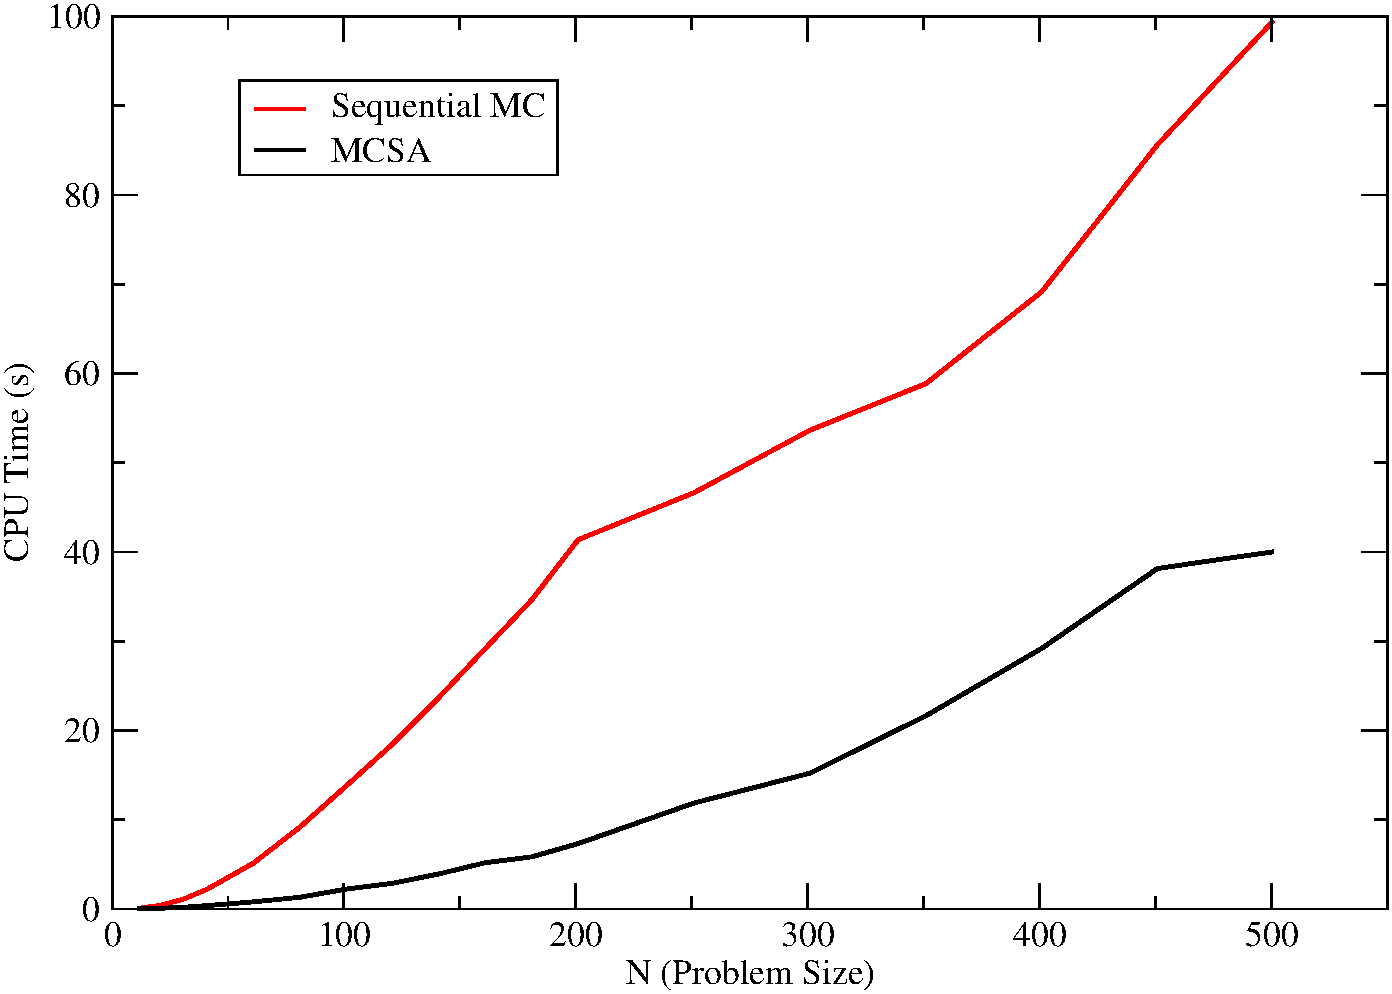
\includegraphics[width=4.5in,clip]{chapters/mc_background/seq_cpu.pdf}
  \caption{\textbf{CPU Time (s) to converge vs. Problem Size ($N$ for
      an $N \times N$ square mesh).} \textit{Both the Sequential Monte
      Carlo and MCSA solvers are used with the five point stencils and
      the adjoint Monte Carlo solver. The number of random walks was
      twice the number of discrete states in the system in order to
      ensure convergence in the Sequential Monte Carlo method.}}
  \label{fig:seq_cpu_time}
\end{figure}

\begin{figure}[t!]
  \centering
  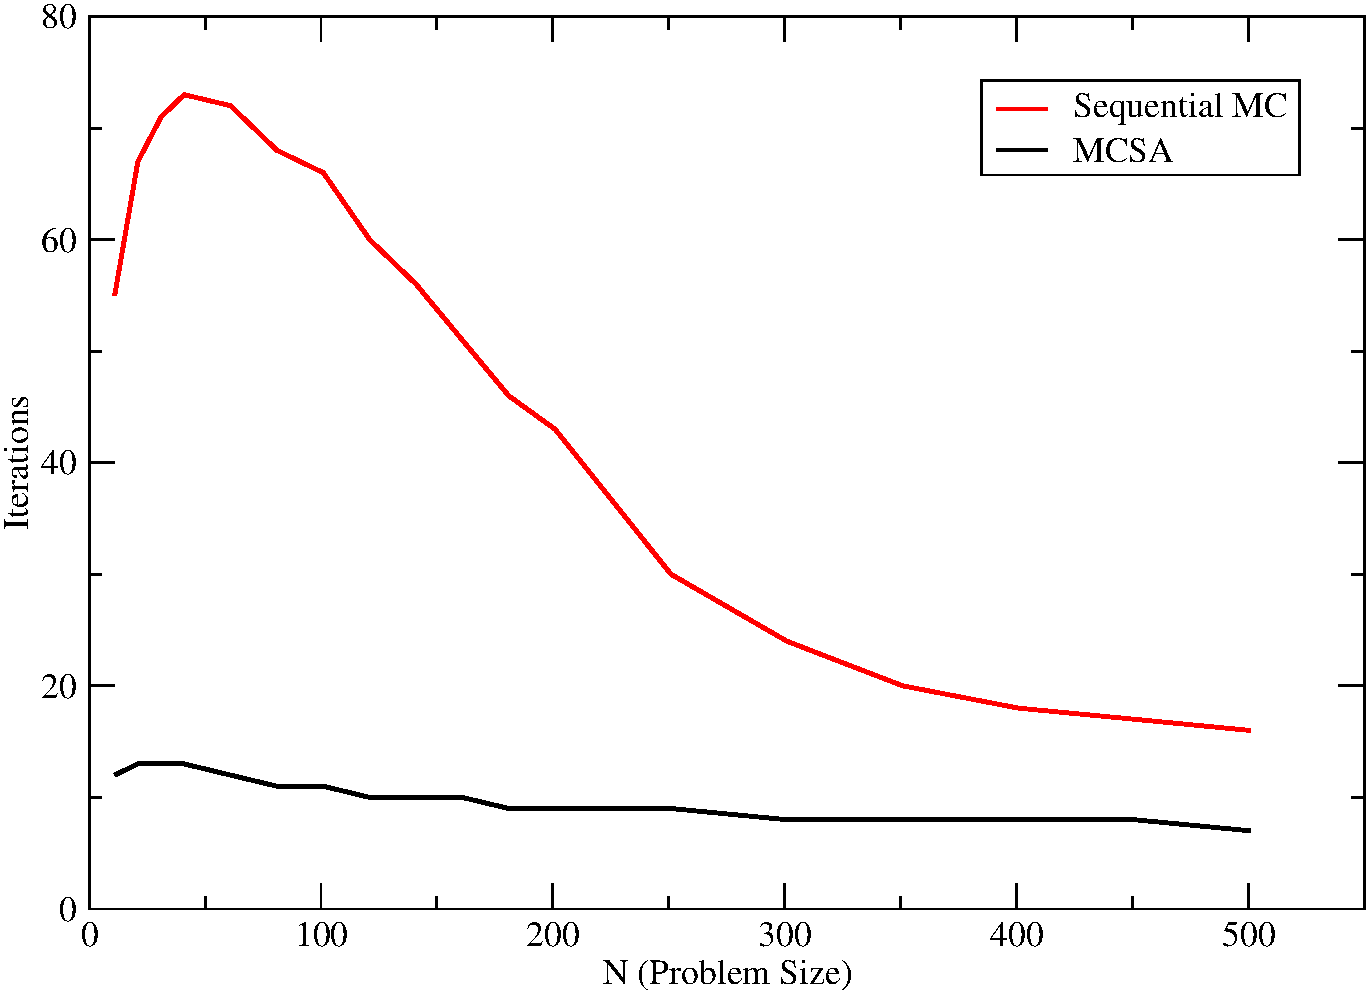
\includegraphics[width=4.5in,clip]{chapters/mc_background/seq_iterations.pdf}
  \caption{\textbf{Iterations to converge vs. Problem Size ($N$ for an
      $N \times N$ square mesh).} \textit{Both the Sequential Monte
      Carlo and MCSA solvers are used with the five point stencils and
      the adjoint Monte Carlo solver.}}
  \label{fig:seq_iterations}
\end{figure}

The benefits of using a synthetic acceleration scheme are also noted
when the infinity norm of the residual computed at each iteration for
both methods was collected at each iteration for a fixed problem sizes
of $N=100$ and $N=500$ as shown in figures Figure~\ref{fig:seq_100}
and \ref{fig:seq_500} respectively. In both cases, the Sequential
method is subject to two regimes of exponential convergence with high
frequency error modes removed in the first regime leaving lower
frequency and slower converging error modes in the second. Using MCSA
we a see a single rate of exponential convergence observed to be much
higher than that computed by Halton's method due to the fact that the
extra Richardson iteration is providing a smoothing effect to
alleviate the error mode variations. Even with the doubling of the
number of stochastic histories computed per time step in order to
ensure convergence for the Sequential method, we still see robustness
issues with a non-monotonically decreasing residual observed for the
$N=100$ case. In both cases the MCSA solver is observed to be robust
with a monotonically decreasing residual.

\begin{figure}[t!]
  \centering
  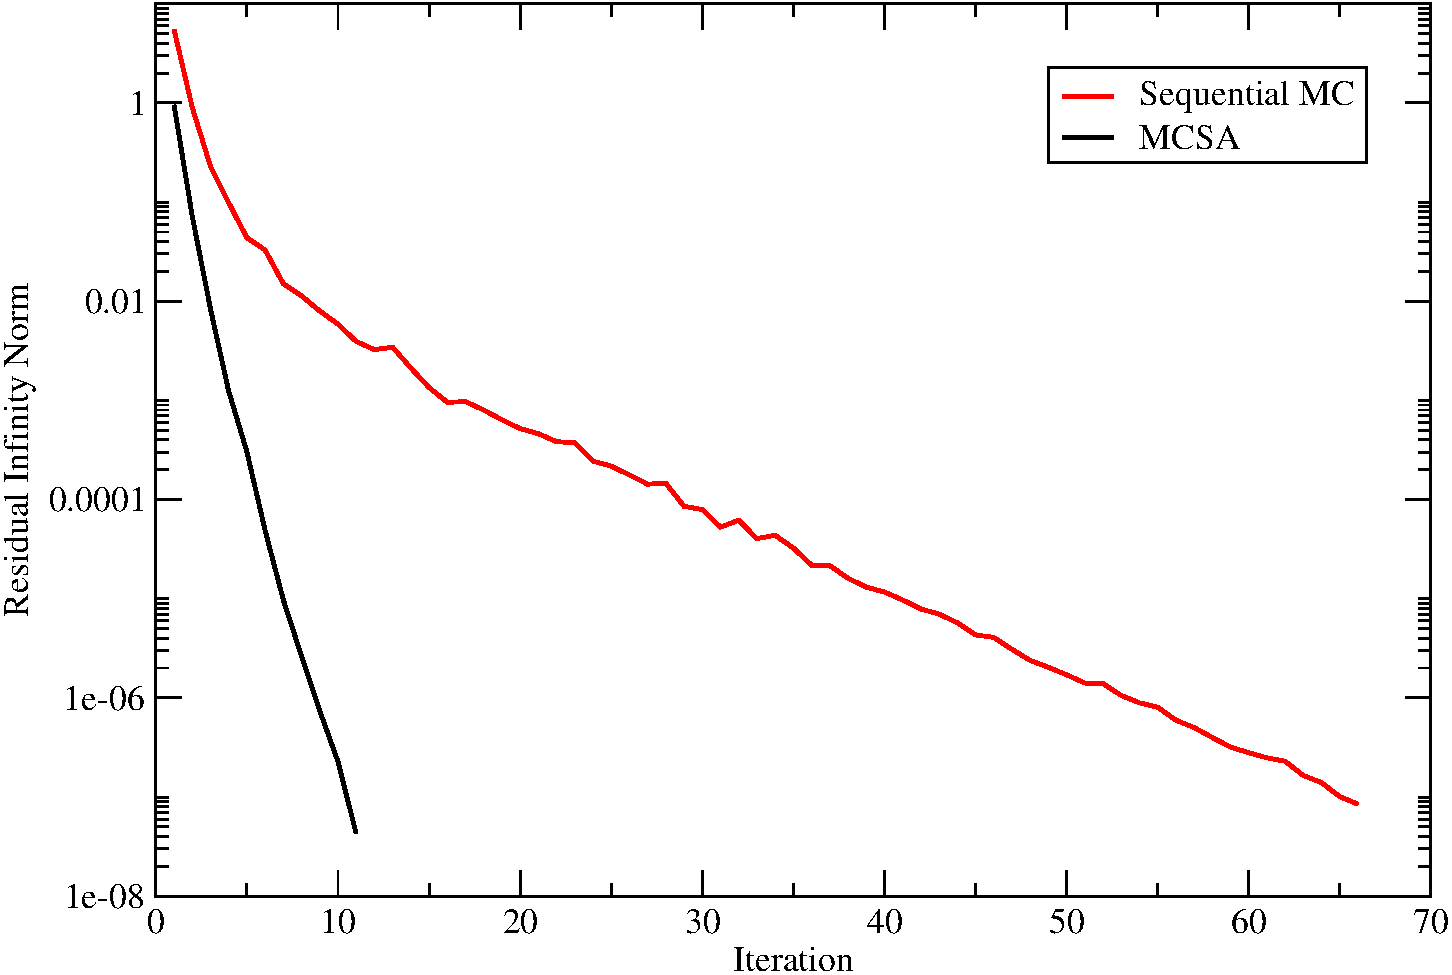
\includegraphics[width=4.5in,clip]{chapters/mc_background/seq_conv_100.pdf}
  \caption{\textbf{Infinity norm of the solution residual
      vs. iteration number for a problem of size $N=100$.}
    \textit{Both the Sequential Monte Carlo and MCSA solvers are used
      with the five point stencils and the adjoint Monte Carlo
      solver.}}
  \label{fig:seq_100}
\end{figure}

\begin{figure}[t!]
  \centering
  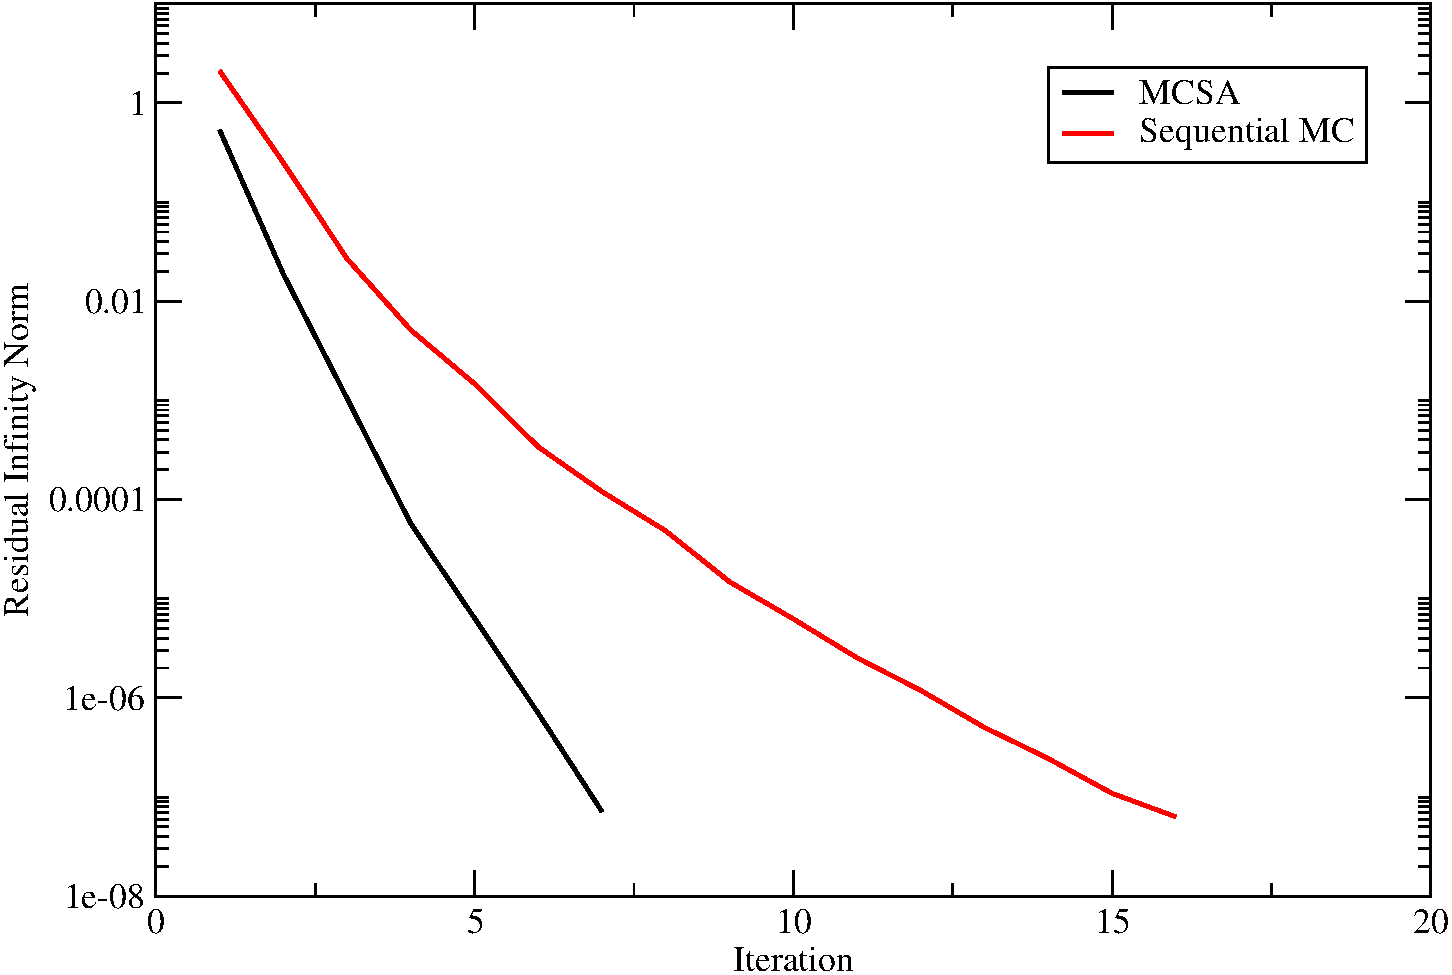
\includegraphics[width=4.5in,clip]{chapters/mc_background/seq_conv_500.pdf}
  \caption{\textbf{Infinity norm of the solution residual
      vs. iteration number for a problem of size $N=500$.}
    \textit{Both the Sequential Monte Carlo and MCSA solvers are used
      with the five point stencils and the adjoint Monte Carlo
      solver.}}
  \label{fig:seq_500}
\end{figure}

\clearpage

\subsection{Monte Carlo Parameter and Estimator Analysis}
\label{sec:parameter_estimator_analysis}
We now study the effects of the adjoint Monte Carlo parameters, weight
cutoff and number of histories, on MCSA performance with both the
collision and expected value estimators. With the same Poisson
problem, we will use a $200 \times 200$ grid and a convergence
tolerance of \sn{1}{-8} for all calculations. To study the effects of
the number of Monte Carlo histories per MCSA iteration, the weight
cutoff was fixed at \sn{1}{-4} while the number of histories per
iteration was varied from 6,000 to 100,000. It was observed that MCSA
would not converge for this problem using the collision estimator with
less than 6,000 histories while the expected value estimator permitted
convergence with only 2,000 histories.

Figure~\ref{fig:estimator_nh_iters} gives the number of iterations
required to converge for both estimators as a function of the number
of histories per iteration. For smaller numbers of histories, the
performance of the expected value estimator is significantly better
than the collision estimator. This result is valuable in that less
transport is required to achieve the same MCSA iterative performance
with the expected value estimator, important for situations where
transport is expensive (i.e. in domain decomposed
calculations). Interestingly, as the number of histories per iteration
are increased, the iterative performance with the collision estimator
approaches that of the expected value estimator. However, given the
performance of the expected value estimator at a fractional number of
histories, one should strongly consider its use over using the
collision estimator with more histories. The CPU time required to
converge is presented in Figure~\ref{fig:estimator_nh_time} and
reflects the results of the iterative performance. In general, using
the collision estimator is slightly slower overall, but the time per
iteration is faster due to the fact that the estimator does not have
to cycle through multiple states during the tally procedure.

\begin{figure}[t!]
  \centering
  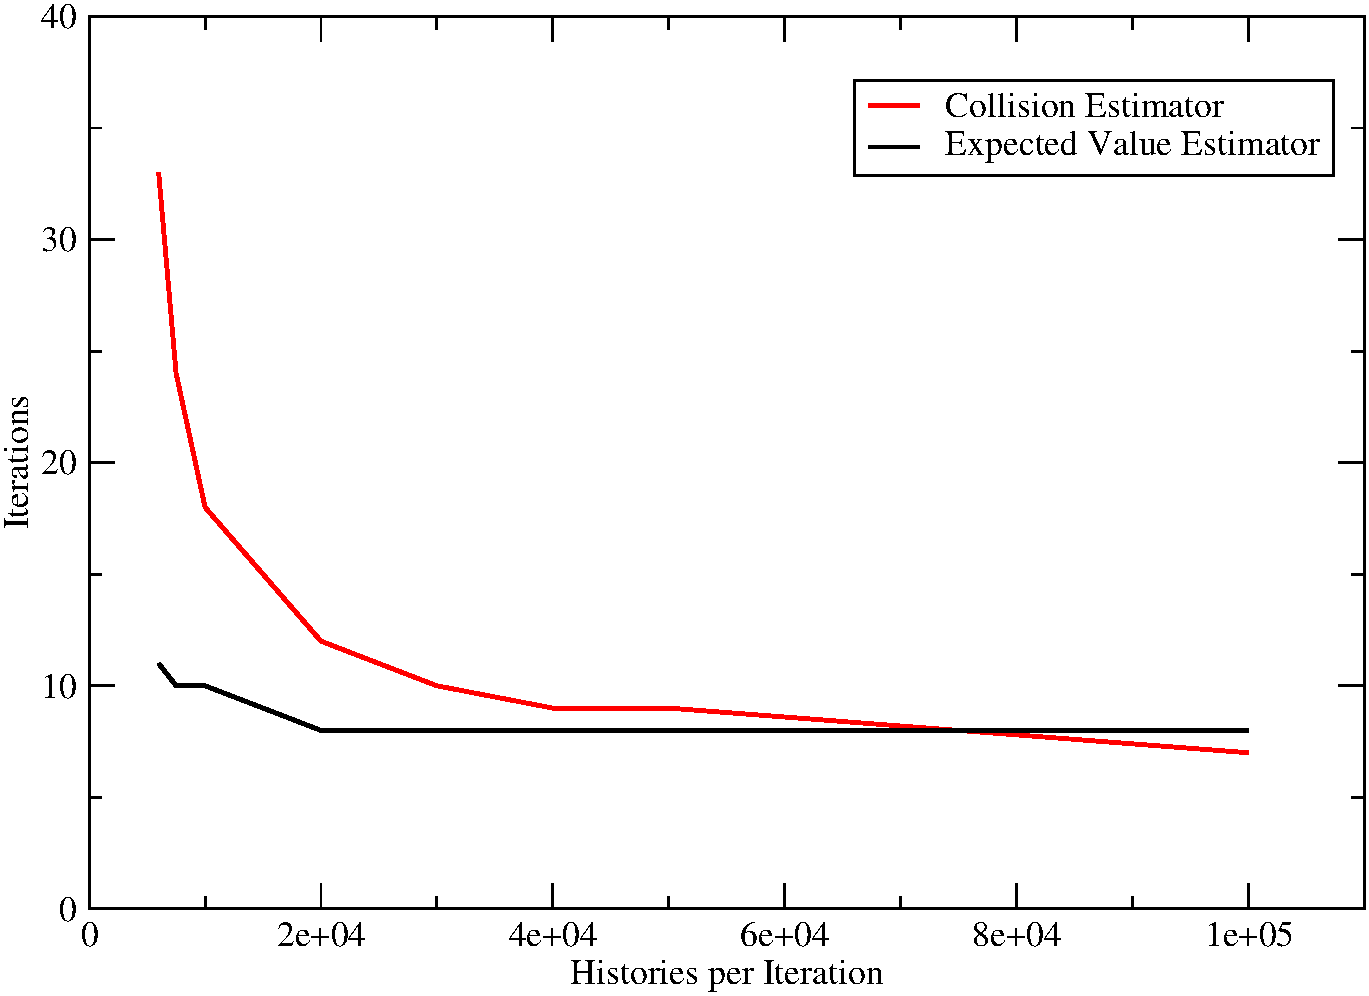
\includegraphics[width=4.75in,clip]{chapters/mc_background/estimator_nh_iters.pdf}
  \caption{\textbf{Iterations (s) to converge vs. Monte Carlo
      histories per MCSA iteration for a $200 \times 200$ square mesh
      and a weight cutoff of \sn{1}{-4}.} \textit{For low numbers of
      histories, the expected value estimator performance is
      significantly better than the collision estimator. At higher
      numbers of histories, the estimators become roughly
      equivalent.}}
  \label{fig:estimator_nh_iters}
\end{figure}

\begin{figure}[t!]
  \centering
  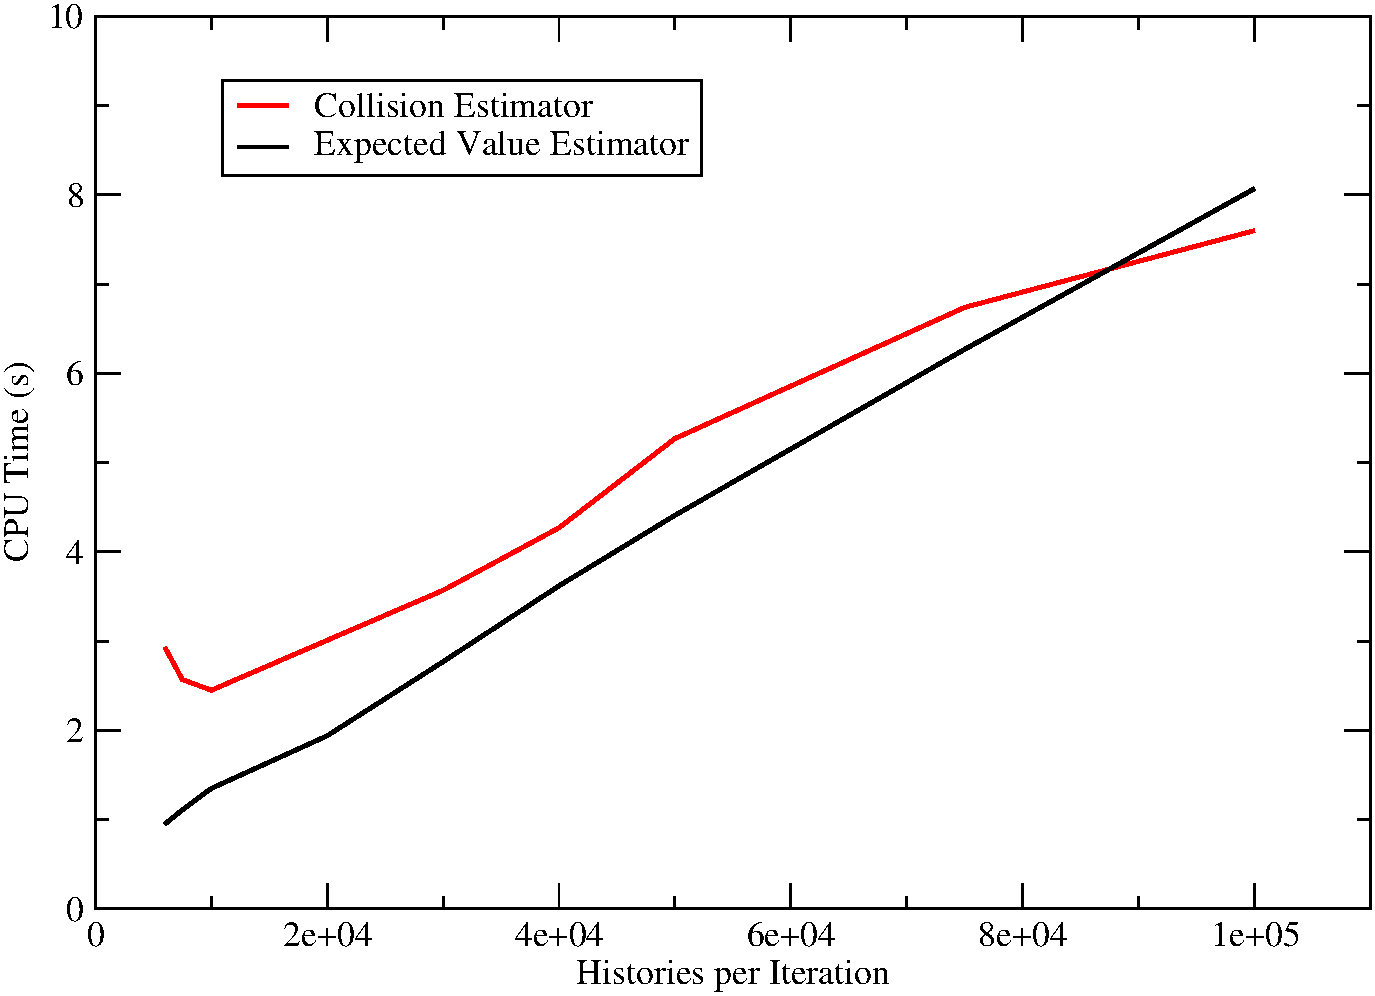
\includegraphics[width=4.75in,clip]{chapters/mc_background/estimator_nh_time.pdf}
  \caption{\textbf{CPU Time (s) to converge vs. Monte Carlo histories
      per MCSA iteration for a $200 \times 200$ square mesh and a
      weight cutoff of \sn{1}{-4}.} \textit{For low numbers of
      histories, the expected value estimator performance is better
      than the collision estimator due to a lower iteration count
      while the actual compute time per iteration is higher.}}
  \label{fig:estimator_nh_time}
\end{figure}

For the weight cutoff study, the number of histories per iteration was
fixed at 40,000 and the weight cutoff varied from \sn{5}{-1} down to
\sn{1}{-10}. Surprisingly, the number of iterations to converge given
by Figure~\ref{fig:estimator_wc_iters} is effectively invariant to the
weight cutoff, only seeing detrimental effects on the number of
iterations at a very large weight cutoff. This suggests that a fairly
large weight cutoff can be used in practice with both adjoint
estimators and that the preliminary components of the random walk are
more important to MCSA convergence than those that occur later and
with lower weight contributions. To further motivate using a larger
weight cutoff, Figure~\ref{fig:estimator_wc_time} gives the CPU time
need to converge as a function of weight cutoff. As expected, lowering
the weight cutoff lengthens the random walk lengths and increases CPU
time at no gain of iterative performance. In general, these results
suggest using the expected value estimator over the collision
estimator with MCSA as well as using a larger weight cutoff.

\begin{figure}[t!]
  \centering
  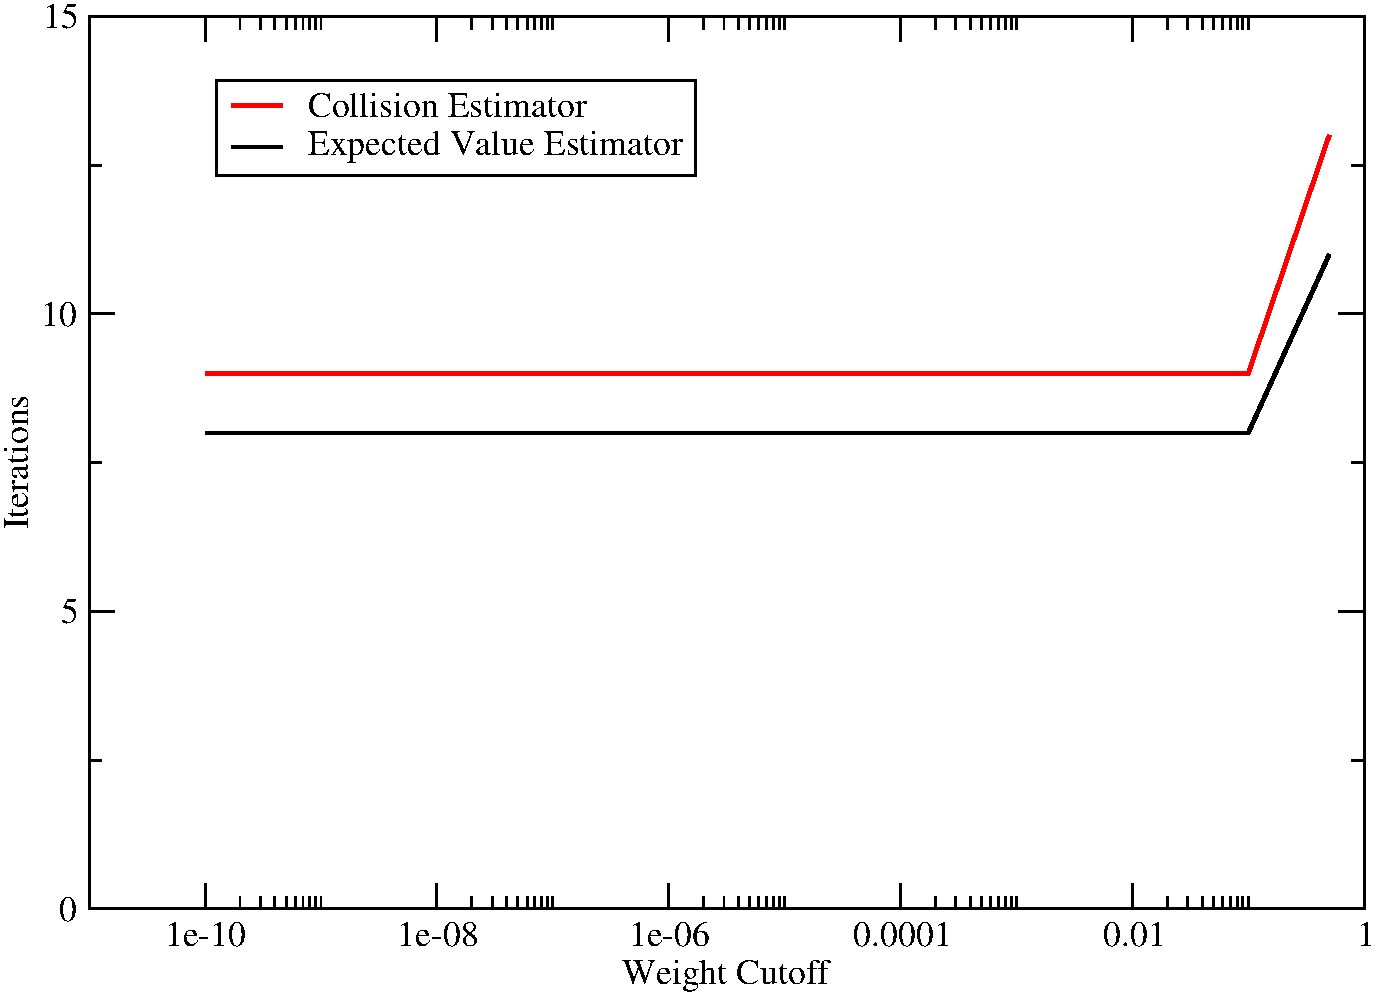
\includegraphics[width=4.75in,clip]{chapters/mc_background/estimator_wc_iters.pdf}
  \caption{\textbf{Iterations (s) to converge vs. history weight
      cutoff for a $200 \times 200$ square mesh and 40,000 histories.}
    \textit{For low numbers of histories, the expected value estimator
      performance is significantly better than the collision
      estimator. At higher numbers of histories, the estimators become
      roughly equivalent.}}
  \label{fig:estimator_wc_iters}
\end{figure}

\begin{figure}[t!]
  \centering
  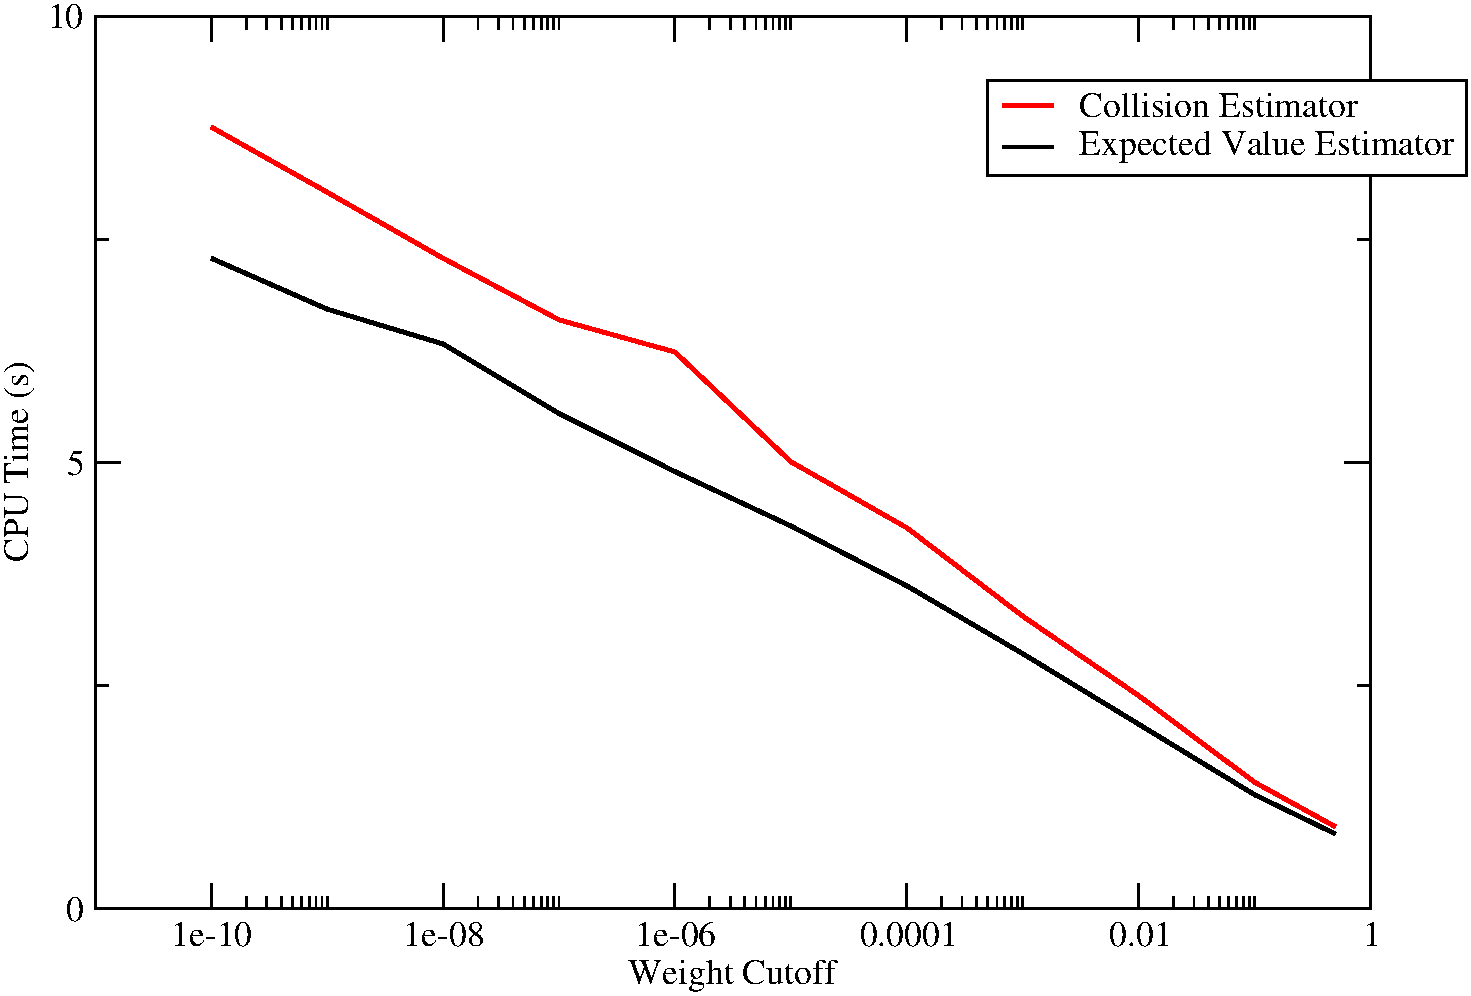
\includegraphics[width=4.75in,clip]{chapters/mc_background/estimator_wc_time.pdf}
  \caption{\textbf{CPU Time (s) to converge vs. history weight cutoff
      for a $200 \times 200$ square mesh and 40,000 histories.}
    \textit{For low numbers of histories, the expected value estimator
      performance is better than the collision estimator due to a
      lower iteration count while the actual compute time per
      iteration is higher.}}
  \label{fig:estimator_wc_time}
\end{figure}

\clearpage

%%---------------------------------------------------------------------------%%
\section{Summary}
\label{sec:mc_summary}

In this chapter, the fundamentals of Monte Carlo Synthetic
Acceleration methods were presented and explored in the context of a
simple model transport system. The following are the significant
observations, findings, and contributions.

\begin{itemize}
\item Monte Carlo Synthetic Acceleration (MCSA) has been generalized
  for all discrete linear transport problems
\item MCSA can be preconditioned using a general left/right scheme but
  requires the explicit inversion of the preconditioners and
  construction of the composite linear operator
\item The adjoint Neumann-Ulam method performs better when used with
  MCSA compared to the forward method
\item MCSA has superior performance when compared to Halton's residual
  Monte Carlo method
\item The Richardson iteration in MCSA behaves as a smoother for the
  stochastic Monte Carlo error
\item MCSA iterative performance when used with the expected value
  estimator is insensitive to histories per iteration
\item MCSA iterative performance is insensitive to the stochastic
  history weight cutoff
\end{itemize}

\chapter{Monte Carlo Synthetic Acceleration\\ Methods for the $SP_N$ Equations}
\label{ch:spn_equations}

In this chapter, we briefly derive the simplified $P_N$ ($SP_N$)
equations, closely following the work of Evans
\cite{evans_simplified_2013}, in order to gain full understanding of
the underlying system and its potential behavior in a Monte Carlo
context. From the $P_N$ equations, we apply a set of approximations to
yield the $SP_N$ equations for fixed source and criticality
problems. Using the fully-formed linear operator for the transport
problem, we explore solutions to the $SP_N$ equations with Monte Carlo
Synthetic Acceleration using a challenging light water reactor fuel
assembly criticality calculation as the driving problem. Several
difficulties arise when applying MCSA to these problems that were not
observed when investigating the simple transport system in the
previous chapter.

For Jacobi-based preconditioners, convergence with MCSA is difficult
if not impossible for ill-conditioned systems with this behavior
demonstrated using a simple neutron diffusion problem. In order to
effectively solve the $SP_N$ equations for the fuel assembly problem,
a suite of preconditioners along with a relaxation scheme is developed
and studied within the context of MCSA. Using these preconditioners,
several additional issues are observed and alleviated to a certain
extent by applying the reduced domain approximation. MCSA solutions
for the fuel assembly problem are then verified by comparing the
solutions against production Krylov solvers for problems with varying
numbers of energy groups. Finally performance is analyzed through
comparison with those same Krylov solvers in terms of both iterative
performance and CPU timing using the same set of problems utilized for
the verification.

%%---------------------------------------------------------------------------%%
\section{The Neutron Transport Equation}
\label{sec:transport_eq}
As a starting point for the $SP_N$ equations we define the
time-independent neutron transport equation
\cite{lewis_computational_1993}:
\begin{multline}
  \hat{\Omega} \cdot \vec{\nabla} \psi(\vec{r},\hat{\Omega},E) +
  \sigma(\vec{r},E) \psi(\vec{r},\hat{\Omega},E) = \\ \iint
  \sigma_s(\vec{r},E' \rightarrow E,\hat{\Omega}' \cdot \hat{\Omega})
  \psi(\vec{r},\hat{\Omega}',E') d\Omega' dE' +
  q(\vec{r},\hat{\Omega},E)\:,
  \label{eq:general_transport}
\end{multline}
with the variables defined as:
\begin{itemize}
\item $\vec{r}$ - neutron spatial position
\item $\hat{\Omega}$ - neutron streaming direction with radial
  component $\mu$ and azimuthal component $\omega$
\item $\hat{\Omega}' \cdot \hat{\Omega} = \mu_0$ is the angle of
  scattering
\item $E$ - neutron energy
\item $\psi(\vec{r},\hat{\Omega},E)$ - angular flux
\item $\sigma(\vec{r},E)$ - total interaction cross section
\item $\sigma_s(\vec{r},E' \rightarrow E,\hat{\Omega}')$ - probability
  of scattering from direction $\hat{\Omega}'$ into an angular domain
  $d\hat{\Omega}'$ about the direction $\hat{\Omega}$ and from energy
  $E'$ to an energy domain $dE'$ about energy $E$
\item $q(\vec{r},\hat{\Omega},E)$ - external source of neutrons.
\end{itemize}
For this work, it is sufficient to formulate
Eq~(\ref{eq:general_transport}) in 1-dimensional Cartesian geometry:
\begin{multline}
  \mu \frac{\partial}{\partial x} \psi(x,\mu,E) + \sigma(x,E)
  \psi(x,\mu,E) = \\ \iint \sigma_s(x,E' \rightarrow E,\hat{\Omega}'
  \cdot \hat{\Omega}) \psi(x,\hat{\Omega}',E') d\Omega' dE' +
  \frac{q(x,E)}{4 \pi}\:,
  \label{eq:cart_1d_transport}
\end{multline}
where the angular component of the solution is no longer dependent on
the azimuthal direction of travel and an isotropic source of neutrons
is assumed. In addition, for fission systems the eigenvalue form of
the transport equation is:
\begin{multline}
  \hat{\Omega} \cdot \vec{\nabla} \psi(\vec{r},\hat{\Omega},E) +
  \sigma(\vec{r},E) \psi(\vec{r},\hat{\Omega},E) = \\ \iint
  \sigma_s(\vec{r},E' \rightarrow E,\hat{\Omega}' \cdot \hat{\Omega})
  \psi(\vec{r},\hat{\Omega}',E') d\Omega' dE' + \\ \frac{1}{k} \chi(E)
  \iint \nu \sigma_f(\hat{r},E') \psi(\vec{r},\hat{\Omega}',E')
  d\Omega' dE' + q(\vec{r},\hat{\Omega},E) \:,
  \label{eq:eigenvalue_transport}
\end{multline}
with the additional variables defined as
\begin{itemize}
\item $k$ - multiplication factor
\item $\chi(E)$ - fission neutron energy spectrum
\item $\nu$ - average number of neutrons per fission
\item $\sigma_f(r,E')$ - fission cross section\:.
\end{itemize}
In 1-dimensional Cartesian geometry,
Eq~(\ref{eq:eigenvalue_transport}) becomes:
\begin{multline}
  \mu \frac{\partial}{\partial x} \psi(x,\mu,E) + \sigma(x,E)
  \psi(x,\mu,E) = \\ \iint \sigma_s(x,E' \rightarrow
  E,\hat{\Omega}' \cdot \hat{\Omega}) \psi(x,\hat{\Omega}',E')
  d\Omega' dE' + \\ \frac{1}{k} \chi(E)
  \iint \nu \sigma_f(x,E') \psi(x,\hat{\Omega}',E') d\Omega'
  dE' + \frac{q(x,E)}{4 \pi}\:.
  \label{eq:cart_1d_eigenvalue}
\end{multline}

%%---------------------------------------------------------------------------%%
\section{Derivation of the Monoenergetic $SP_N$ Equations}
\label{sec:spn_equations}
The $P_N$ equations as derived in \cite{lewis_computational_1993}
give $N+1$ coupled first-order equations capturing the spatial and
angular-dependence of the solution:
\begin{equation}
   \frac{1}{2n+1} \frac{\partial}{\partial x}\Big[ (n+1) \phi_{n+1} + n
     \phi_{n-1} \Big] + \Sigma_n \phi_n = q\delta_{n0} \:,
  \label{eq:final_pn_equations}
\end{equation}
where $\Sigma_n = \sigma-\sigma_{sn}$ and the summations are truncated
at some level of approximation $N$ such that $n = 0,1,\dotsc,N$. This
yields a set of $N+1$ equations for $N+2$ flux moments with the
highest order moment set to zero for closure. In multiple dimensions,
the equation set becomes large and coupled not only through angular
moments but also through the spatial variables. As a simpler
alternative to multidimensional $P_N$ solutions, Gelbard recognized in
1960 that the planar $P_N$ equations could be simplified and applied
an ad-hoc method to extend them to multiple dimensions, yielding the
$SP_N$ equations. These equations are not only fewer in number, but
also take on a diffusion-like form while maintaining the angular
character of the flux, making them amenable to solutions with modern
diffusion methods.

First, the $P_N$ equations can be simplified to $(N+1)/2$ second-order
equations by solving for the $n^{th}$ Legendre flux moment in the
odd-order equations:
\begin{equation}
  \phi_n = \frac{1}{\Sigma_n}\Bigg[ q \delta_{no} -
    \frac{\partial}{\partial x}\Big(\frac{n}{2n+1}\phi_{n-1} +
    \frac{n+1}{2n+1} \phi_{n+1} \Big) \Bigg]\:, 
  \label{eq:odd_moments}
\end{equation}
for $n = 1,3,\cdots,N$ and $\delta_{no} = 0\ \forall n \neq 0$. We can
insert the odd moments into Eq~(\ref{eq:final_pn_equations}) to get a
reduced group of equations for the even moments:
\begin{multline}
  -\frac{\partial}{\partial x}
  \Bigg[\frac{n}{2n+1}\frac{1}{\Sigma_{n-1}} \frac{\partial}{\partial
      x} \Big(\frac{n-1}{2n-1} \phi_{n-2} + \frac{n}{2n-1}\phi_n \Big)
    \\+ \frac{n+1}{2n+1}\frac{1}{\Sigma_{n+1}} \frac{\partial}{\partial
      x} \Big(\frac{n+1}{2n+3}\phi_n + \frac{n+2}{2n+3}\phi_{n+2}\Big)
    \Bigg] \\+ \Sigma_n \phi_n = q \delta_{n0}\ \ \ \ \ \ \ \ \ n =
  0,2,4,\cdots,N\:.
  \label{eq:reduced_pn}
\end{multline}
To extend these equations to multiple dimensions, Gelbard simply
replaced the planar spatial derivatives in the reduced set of
equations with general multidimensional gradient operators:
\begin{multline}
  -\nabla \cdot \Bigg[\frac{n}{2n+1}\frac{1}{\Sigma_{n-1}} \nabla
    \Big(\frac{n-1}{2n-1} \phi_{n-2} + \frac{n}{2n-1}\phi_n \Big) \\+
    \frac{n+1}{2n+1}\frac{1}{\Sigma_{n+1}} \nabla
    \Big(\frac{n+1}{2n+3}\phi_n + \frac{n+2}{2n+3}\phi_{n+2}\Big)
    \Bigg] \\+ \Sigma_n \phi_n = q \delta_{n0}\ \ \ \ \ \ \ \ \ n =
  0,2,4,\cdots,N\:,
  \label{eq:spn_equations}
\end{multline}
yielding a multidimensional set of $(N+1)/2$ angular coupled equations
defined as the $SP_N$ equations. As with the $P_N$ equations, we
provide closure to this set of equations with $\phi_{N+1} = 0$. As a
concrete example, we will consider the $SP_7$ equations:
\begin{subequations}
  \begin{gather}
    -\nabla \cdot \frac{1}{3 \Sigma_1} \nabla ( \phi_0 + 2\phi_2 ) +
    \Sigma_0 \phi_0 = q \\ 
    -\nabla \cdot \Bigg[ \frac{2}{15 \Sigma_1} \nabla ( \phi_0 + 2\phi_2
      ) + \frac{3}{35 \Sigma_3}\nabla( 3\phi_2 + 4\phi_4)\Bigg] +
    \Sigma_2 \phi_2 = 0\\
    -\nabla \cdot \Bigg[ \frac{4}{63 \Sigma_3} \nabla ( 3\phi_2 +
      4\phi_4 ) + \frac{5}{99 \Sigma_5}\nabla( 5\phi_4 +
      6\phi_6)\Bigg] + \Sigma_4 \phi_4 = 0\\
    -\nabla \cdot \Bigg[ \frac{6}{143 \Sigma_5} \nabla ( 5\phi_4 +
      6\phi_6 ) + \frac{7}{195 \Sigma_7}\nabla(7\phi_6)\Bigg] +
    \Sigma_6 \phi_6 = 0 \:.
  \end{gather}
  \label{eq:sp7_equations}
\end{subequations}
To further modify these equations, we can use a change of variables to
create a new group of equations such that the gradients are operating
on a single vector:
\begin{subequations}
  \begin{gather}
    u_1 = \phi_0 + 2\phi_2 \\
    u_2 = 3\phi_2 + 4\phi_4 \\
    u_3 = 5\phi_4 + 6\phi_6 \\
    u_4 = 7\phi_6 \:.
  \end{gather}
  \label{eq:spn7_subs}
\end{subequations}
When substituted into Eq~(\ref{eq:sp7_equations}), these terms give:
\begin{subequations}
  \begin{gather}
    -\nabla \cdot \frac{1}{3 \Sigma_1} \nabla u_1 + \Sigma_0 \Bigg[
    u_1 - \frac{2}{3}u_2 + \frac{8}{15}u_3 - \frac{16}{35}u_4 \Bigg]
    = -q \\
    -\nabla \cdot \Bigg[ \frac{2}{15 \Sigma_1} \nabla u_1 +
    \frac{3}{35 \Sigma_3} \nabla u_2 \Bigg] + \Sigma_2 \Bigg[
    \frac{1}{3}u_2 - \frac{4}{15}u_3 + \frac{8}{35}u_4 \Bigg] = 0 \\
    -\nabla \cdot \Bigg[ \frac{4}{63 \Sigma_3} \nabla u_2 +
    \frac{5}{99 \Sigma_5} \nabla u_3 \Bigg] + \Sigma_4 \Bigg[
    \frac{1}{5}u_3 - \frac{6}{35}u_4 \Bigg] = 0 \\ 
    -\nabla \cdot \Bigg[ \frac{6}{143 \Sigma_5} \nabla u_3 +
    \frac{7}{195 \Sigma_7} \nabla u_4 \Bigg] + \Sigma_6 \Bigg[
    \frac{1}{7}u_4 \Bigg] = 0 \:.
  \end{gather}
  \label{eq:spn7_subs_equations}
\end{subequations}
If we rearrange Eq~(\ref{eq:spn7_subs_equations}) such that only one
divergence operation is present in each equation, we can formulate
this as a matrix system of 4 equations in the case of the $SP_7$
approximation:
\begin{equation}
  -\nabla \cdot D_n \nabla u_n + \sum_{m=1}^4 A_{nm} u_m =
  q_n\ \ \ \ \ \ \ n = 1,2,3,4\:,
  \label{eq:spn_matrix}
\end{equation}
with $\mathbf{u}$ the vector of solution variables:
\begin{equation}
  \mathbf{u} = ( u_1\ \ u_2\ \ u_3\ \ u_4 )^T \:,
  \label{eq:spn7_solution_vector}
\end{equation}
$\mathbf{D}$ the vector of effective diffusion coefficients:
\begin{equation}
  \mathbf{D} = \Bigg( \frac{1}{3\Sigma_1}\ \ \frac{1}{7\Sigma_3}\ \
  \frac{1}{11\Sigma_5}\ \ \frac{1}{15\Sigma_7} \Bigg)^T\:,
  \label{eq:spn7_diffusion_coeffs}
\end{equation}
$\mathbf{q}$ the vector of source terms where the $0^{th}$ moment
source has now been distributed through the system:
\begin{equation}
  \mathbf{q} = (
  q\ \ -\frac{2}{3}q\ \ \frac{8}{15}q\ \ -\frac{16}{35}q )^T\:,
  \label{eq:spn7_source_vector}
\end{equation}
and $\mathbf{A}$ a matrix of angular scattering terms:
% NOTE: I copied the following matrix directly out of Tom's tech note
% on the SPn equations.
\begin{equation}
  \mathbf{A} = 
  {\tiny \begin{bmatrix}
    (\Sigma_0) &
    (-\frac{2}{3}\Sigma_0) &
    (\frac{8}{15}\Sigma_0) &
    (-\frac{16}{35}\Sigma_0) \\
    %%
    &&&\\
    %%
    (-\frac{2}{3}\Sigma_0) &
    (\frac{4}{9}\Sigma_0 + \frac{5}{9}\Sigma_2) &
    (-\frac{16}{45}\Sigma_0 - \frac{4}{9}\Sigma_2) &
    (\frac{32}{105}\Sigma_0 + \frac{8}{21}\Sigma_2) \\
    %%
    &&&\\
    %%
    (\frac{8}{15}\Sigma_0) &
    (-\frac{16}{45}\Sigma_0 - \frac{4}{9}\Sigma_2) &
    (\frac{64}{225}\Sigma_0 + \frac{16}{45}\Sigma_2 + \frac{9}{25}\Sigma_4) &
    (-\frac{128}{525}\Sigma_0 - \frac{32}{105}\Sigma_2 - \frac{54}{175}\Sigma_4)
    \\ 
    %%
    &&&\\
    %%
    (-\frac{16}{35}\Sigma_0) &
    (\frac{32}{105}\Sigma_0 + \frac{8}{21}\Sigma_2) &
    (-\frac{128}{525}\Sigma_0 - \frac{32}{105}\Sigma_2 - \frac{54}{175}\Sigma_4)
    & 
    (\frac{256}{1225}\Sigma_0 + \frac{64}{245}\Sigma_2 +
    \frac{324}{1225}\Sigma_4 + \frac{13}{49}\Sigma_6)
  \end{bmatrix}}\:.
  \label{eq:A_matrix}
\end{equation}
Note that the term $\sum_{m=1}^4 A_{nm} u_m$ in
Eq~(\ref{eq:spn_matrix}) couples the moments in each equation while
the diffusive term in each equation is only for a single
'pseudo-moment' $u_n$. As noted by Evans \cite{evans_simplified_2013},
lower order $SP_N$ approximations can be generated by setting higher
order even moments in this system to zero (e.g. $\phi_6 = \phi_4 = 0$
yields the $SP_3$ equations). For these equations, the $SP_N$ order
defines the largest order flux moment maintained in the calculation
and the $P_N$ order defines the largest order of the cross section
expansion maintained.

\subsection{Eigenvalue Form of the $SP_N$ Equations}
\label{subsec:eigenvalue_form}
For criticality problems, the space, angle, and energy discretizations
for the $SP_N$ equations can be applied to the general eigenvalue form
of the transport equation given by
Eq~(\ref{eq:eigenvalue_transport}). We can readily replace the fixed
source in Eq~(\ref{eq:spn_matrix}) with a fission source this time
considering the multigroup form of the $SP_N$ equations derived in
Appendix~\ref{chap:mg_spn_equations}:
\begin{multline}
  -\nabla \cdot \Bigg[\frac{n}{2n+1}\mathbf{\Sigma_{n-1}}^{-1} \nabla
    \Big(\frac{n-1}{2n-1} \mathbf{\Phi_{n-2}} +
    \frac{n}{2n-1}\mathbf{\Phi_n} \Big) \\+
    \frac{n+1}{2n+1}\mathbf{\Sigma_{n+1}}^{-1} \nabla
    \Big(\frac{n+1}{2n+3}\mathbf{\Phi_n} +
    \frac{n+2}{2n+3}\mathbf{\Phi_{n+2}}\Big) \Bigg] \\+
  \mathbf{\Sigma_n} \mathbf{\Phi_n} = \frac{1}{k} \mathbf{F}
  \mathbf{\Phi_n} \delta_{n0} \ \ \ \ \ \ \ \ \ n = 0,2,4,\cdots,N\:.
  \label{eq:multigroup_spn_eigenvalue}
\end{multline}
with $\mathbf{\Phi_n}$ the vector of multigroup flux moments and the
fission matrix, $\mathbf{F}$, given by
\cite{evans_simplified_2013}. We again apply the change of variables
to yield the set of multigroup pseudo-moments $\mathbb{U}_n$ where now
the application of the fission matrix to the moment vectors will be
expanded into a set of block matrices in identical fashion to the
scattering matrices:
\begin{equation}
  -\nabla \cdot \mathbb{D}_n \nabla \mathbb{U}_n + \sum_{m=1}^4
  \mathbb{A}_{nm} \mathbb{U}_m = \frac{1}{k} \sum_{m=1}^4
  \mathbb{F}_{nm} \mathbb{U}_m\ \ \ \ \ \ \ n = 1,2,3,4\:.
  \label{eq:spn_fission_matrix}
\end{equation}
To complete the spatial discretization, the gradient operators are
resolved by a finite volume scheme as in
\cite{evans_simplified_2013}. It should be noted here that with
respect to a general MCSA scheme, the introduction of fission in the
system will only affect the source vector in the linear system for the
eigenvalue schemes used in this work. The linear operator, and
therefore overall MCSA performance will be dictated by streaming and
scattering as defined on the left-hand side.

%%---------------------------------------------------------------------------%%
\section{Fuel Assembly Criticality Calculations}
\label{sec:fuel_assembly_calcs}
Fuel assembly calculations are a critical piece of nuclear engineering
infrastructure for reactor core analysis and design. At this level,
individual fuel pins may be resolved at fine resolution in a variety
of configurations. As a sophisticated problem of interest to push the
limits of MCSA, a hot zero-power $17 \times 17$ pin assembly will be
used with varying energy group structure and $SP_N$ discretization in
a criticality calculation. A cross section along the vertical axis
showing homogenized fuel pin, control rod, and moderator materials and
the associated grid is given by Figure~\ref{fig:problem3_radial_mat}
while a cross section of the materials configuration along the
horizontal axis is given by Figure~\ref{fig:problem3_axial_mat}. The
control rods were removed for these problems leaving only moderator in
their place. A detailed view of the assembly bottom is given in
Figure~\ref{fig:problem3_end}. On the top and bottom of the assembly,
vacuum conditions are used as well as on the top and right boundaries
in Figure~\ref{fig:problem3_radial_mat}. Reflecting conditions are
used on the left and bottom boundaries of
Figure~\ref{fig:problem3_radial_mat}, effectively giving a
representation of one quarter of the assembly. For the spatial
discretization, each fuel pin (gray regions in
Figure~\ref{fig:problem3_radial_mat}) is resolved by a $2 \times 2$
mesh with materials and cross sections homogenized over this region.
\begin{figure}[t!]
  \begin{center}
    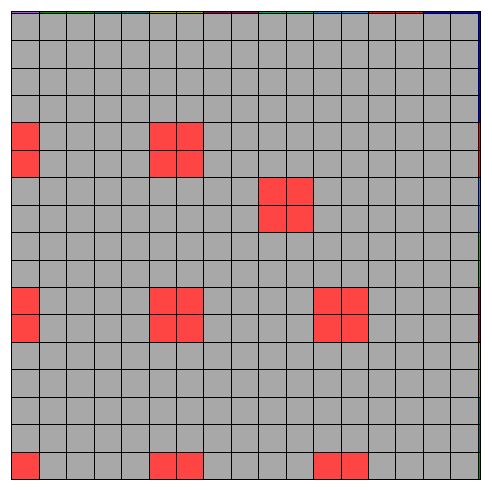
\includegraphics[width=4in]{chapters/spn_equations/problem3_radial_mat.png}
  \end{center}
  \caption{\textbf{Fuel assembly mesh and geometry cross section.}
    \textit{Reflecting boundaries are used on the left and lower
      boundaries to create a complete $17 \times 17$ assembly
      geometry. Gray regions are homogenized fuel and red regions are
      homogenized control rods. Each fuel pin is resolved by a $2
      \times 2$ mesh.}}
  \label{fig:problem3_radial_mat}
\end{figure}
\begin{figure}[t!]
  \begin{center}
    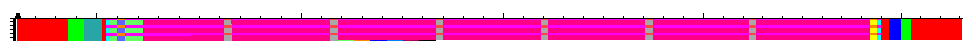
\includegraphics[width=6.0in]{chapters/spn_equations/problem3_axial_mat.png}
  \end{center}
  \caption{\textbf{Fuel assembly geometry cross section.} \textit{The
      geometry is subdivided along the axial direction into 50 zones
      spaced to capture material boundaries. Important details include
      spacer grids along the length of the fuel pins and reactor core
      structures on the top and bottom of the assembly. Lighter purple
      material in the center of the assembly is homogenized
      moderator/control rodes and darker purple/red material is
      homogenized moderator/fuel.}}
  \label{fig:problem3_axial_mat}
\end{figure}
\begin{figure}[t!]
  \begin{center}
    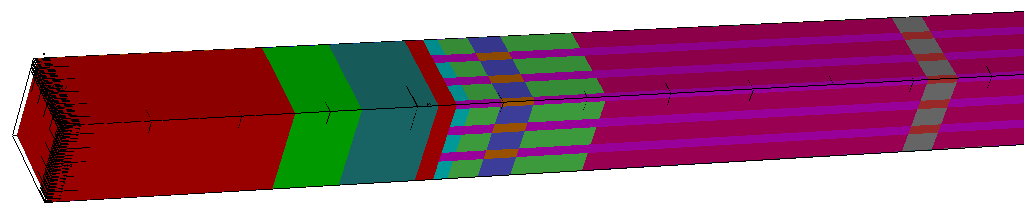
\includegraphics[width=6.0in]{chapters/spn_equations/problem3_end.png}
  \end{center}
  \caption{\textbf{Fuel assembly geometry end detail.}
    \textit{Reactor core structure including spacer grids and plenum
      has been included. Lighter purple material on the right of the
      figure is homogenized moderator/control rods and darker
      purple/red material is homogenized moderator/fuel.}}
  \label{fig:problem3_end}
\end{figure}

Significant geometric details are contained in the model including
spacer grids, fuel pins with homogenized cladding and gas gap, core
plenum, and moderator with boron. Group cross sections and other
discrete nuclear data are generated as needed by a cross-section
processing module dependent on the meshing parameters used to
discretize the geometry and single-dimension pin-cell calculations for
initial flux spectrum generation. Table~\ref{tab:problem3_parameters}
gives the primary design parameters for the fuel assembly
calculations.
\begin{table}[h!]
  \begin{center}
    \begin{tabular}{ll}\hline\hline
      \multicolumn{1}{l}{\textbf{Parameter}} & 
      \multicolumn{1}{l}{\textbf{Value}} \\
      Power Level & 0 MW \\
      Inlet Temperature & 326.85C \\
      Fuel Temperature & 600C \\
      Boron Concentration & 1300 ppm \\
      Moderator Density & 0.743 g/cc \\
      Helium Density & \sn{1.79}{-4} g/cc \\
      Zirconium Density & 6.56 g/cc \\
      Stainless Steel Density & 8.0 g/cc \\
      Inconel Density & 8.19 g/cc \\
      UO2 Density & 10.257 g/cc \\
      Fuel Pin Radius (w/o clad) & 0.4096 cm \\
      %%
      \hline\hline
    \end{tabular}
  \end{center}
  \caption{\textbf{Design parameters for the $17 \times 17$ pin fuel
      assembly criticality calculation.}}
  \label{tab:problem3_parameters}
\end{table}

To generate the multiplication factor and steady-state flux
distribution for this problem, at every eigenvalue iteration MCSA is
used to solve the resulting $SP_N$ problem using the provided fission
source. Algorithm~\ref{alg:power_iteration} presents the use of MCSA
within a power iteration strategy to find the multiplication factor.
\begin{algorithm}[h!]
  \caption{Power Iteration MCSA Scheme}
  \label{alg:power_iteration}
  \begin{algorithmic}
    \State $k_0 =$ initial guess
    \State $\mathbf{\Phi}_0 =$ initial guess
    \State $n = 0$
    \While{$|\frac{k^n - k^{n-1}}{k^n}| < \epsilon$}
    \Comment{Iterate until convergence of the eigenvalue}
    \State $\mathbf{M} \mathbf{\Phi}^{n+1} = \frac{1}{k^n} \mathbf{F} \mathbf{\Phi}^n$
    \Comment{Solve for the new flux state with MCSA}
    \State $k^{n+1} = k^n \frac{\int \mathbf{F} \mathbf{\Phi}^{n+1} d\mathbf{r}}{\int
      \mathbf{F} \mathbf{\Phi}^n d\mathbf{r}}$
    \Comment{Update the multiplication factor}
    \State $n = n+1$
    \EndWhile
  \end{algorithmic}
\end{algorithm}
Here, $\mathbf{M}$ is the transport operator generated on the
left-hand side of the $SP_N$ discretization, $\mathbf{F}$ is the
fission matrix, and $\mathbf{\Phi}$ the multigroup neutron flux. Using
MCSA in this context is significantly more complicated than the simple
test problem used for the previous fixed-source preconditioner
analysis. Fission has been introduced into the set of equations and
the addition of moderator into the system will increase the amount of
scattering, creating a significantly more difficult problem
manifesting itself in an iteration matrix with a larger spectral
radius. When using MCSA, the linear operator applied to
$\mathbf{\Phi}^{n+1}$ at each eigenvalue iteration will dictate
convergence and remain unchanged throughout the eigenvalue computation
while the addition of fission to the system will only modify the
source of neutrons and the multiplication factor at every eigenvalue
iteration while not affecting Monte Carlo transport.
 
\subsection{Block Jacobi Preconditioning}
\label{subsec:spn_spectral_analysis}
Previous work in applying MCSA to the thermal radiation diffusion
equation had success in using Jacobi preconditioning
\cite{evans_monte_2012} and therefore we apply it here to the $SP_N$
equations given their diffusion-like form. In this section, we will
the structure of the transport operator formed by the $SP_N$ equations
while parametrically varying the $SP_N$ order, the $P_N$ order, the
number of energy groups, and upscattering/downscattering between
energy groups. For each basic problem, the values given in
Table~\ref{tab:spn_fixed_parameters} were fixed for each spatial
location and energy group.

\begin{table}[h!]
  \begin{center}
    \begin{tabular}{ll}\hline\hline
      \multicolumn{1}{c}{Parameter}& 
      \multicolumn{1}{c}{Value} \\\hline
      Mesh Element Size & 1.0 \\
      Mesh Elements & $2 \times 2 \times 2$ \\
      Reflecting Boundaries & True \\
      Materials & 1 \\
      Source Strength & 1.0 \\
      Total Cross Section & 5.0 \\
      In-Group Cross Section & 0.25 \\
      Downscatter Cross Section & 1.0 \\
      Upscatter Cross Section & 0.1 \\
      Eigenvalue Solver Tolerance & $1.0\times10^{-8}$ \\
      %%
      \hline\hline
    \end{tabular}
  \end{center}
  \caption{\textbf{Fixed parameters for the $SP_N$ spectral radius
      parameter study.} \textit{The parameters were fixed for each
      spatial location and energy group.}}
  \label{tab:spn_fixed_parameters}
\end{table}

Mesh element sizes were the same in all cardinal directions with
reflecting conditions on each boundary. For the energy parameter, 1
and 10 energy groups were used with upscatter/downscatter varied for
the 10 group case. For the downscatter cases, all groups could scatter
to all lower energy groups with the cross sections given in
Table~\ref{tab:spn_fixed_parameters} while for the upscatter case all
groups could scatter to all other energy groups with different cross
sections for upscatter and downscatter used. A uniform isotropic
source of neutrons is given in each group as well.

The matrices generated by the discretization of this problem are
sparse with a block-based form as dictated by
Eq~(\ref{eq:spn_multigroup_system}). Figure~\ref{fig:group1} gives the
sparsity pattern for a monoenergetic $SP_7$ discretization while
Figures~\ref{fig:group10ds} and \ref{fig:group10us} give the sparsity
patterns for the same problem for 10 energy groups without and with
upscatter respectively.

\begin{figure}[t!]
  \begin{center}
    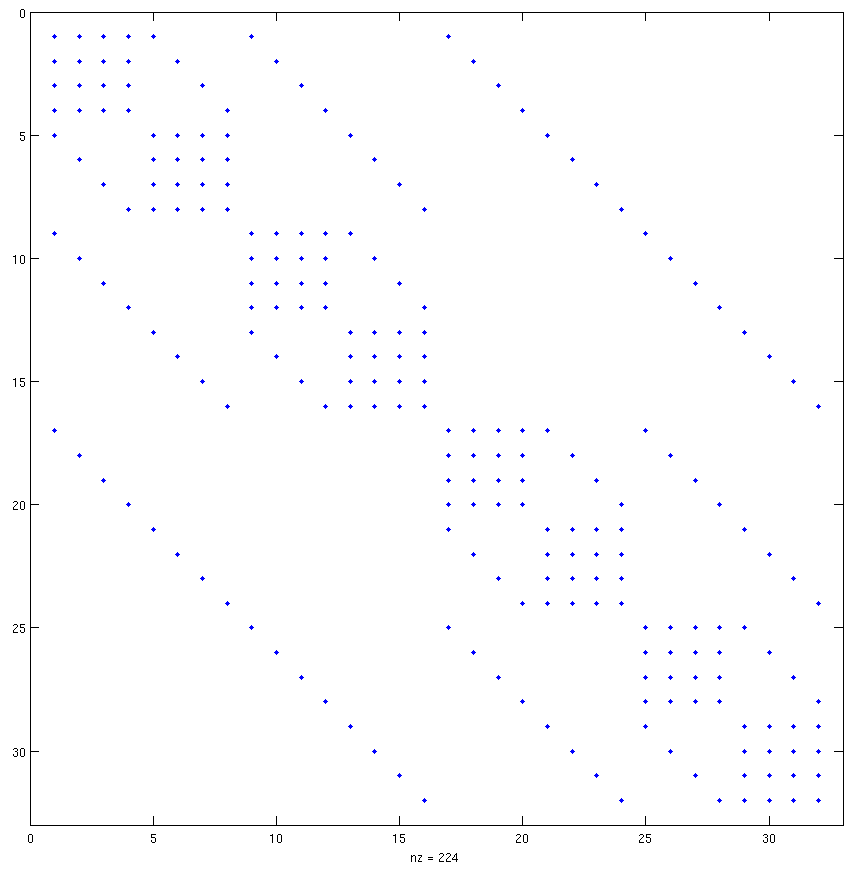
\includegraphics[width=3.3in]{chapters/spn_equations/group1.png}
  \end{center}
  \caption{\textbf{Sparsity pattern for 1-group $SP_7$
      discretization.} \textit{A $2\times 2 \times 2$ element mesh was
      used to show detail of the blocks formed by the discretization.}}
  \label{fig:group1}
\end{figure}
\begin{figure}[t!]
  \begin{center}
    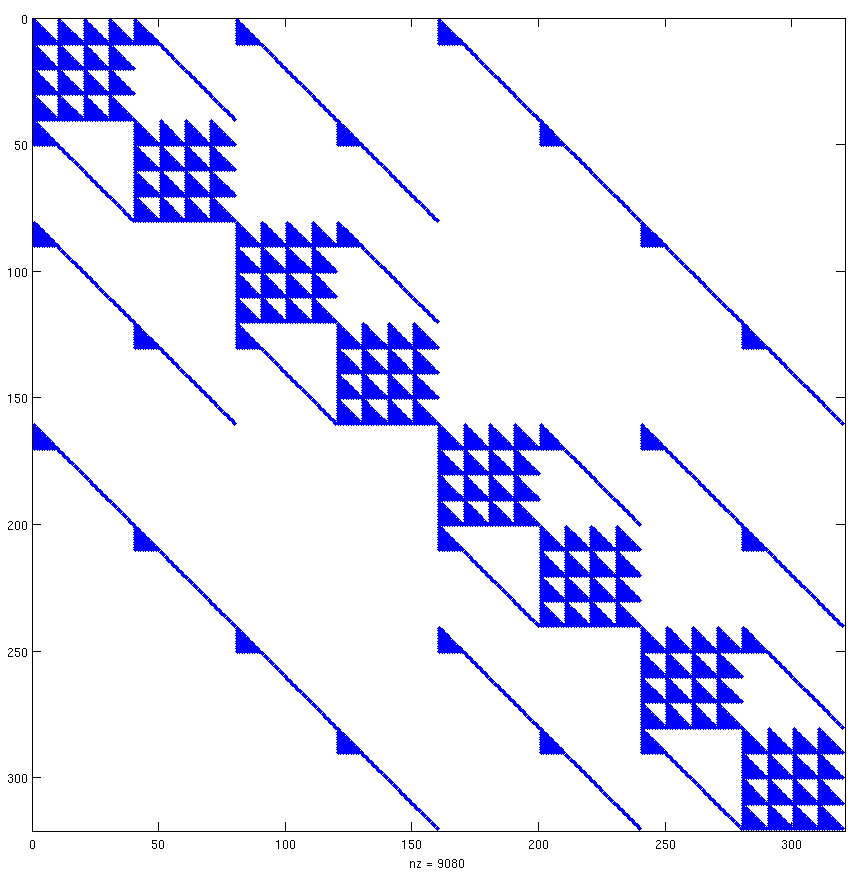
\includegraphics[width=3.3in]{chapters/spn_equations/group10ds.png}
  \end{center}
  \caption{\textbf{Sparsity pattern for 10-group $SP_7$ discretization
      with downscatter only.} \textit{A $2\times 2 \times 2$ element
      mesh was used to show detail of the blocks formed by the
      discretization.}}
  \label{fig:group10ds}
\end{figure}
\begin{figure}[t!]
  \begin{center}
    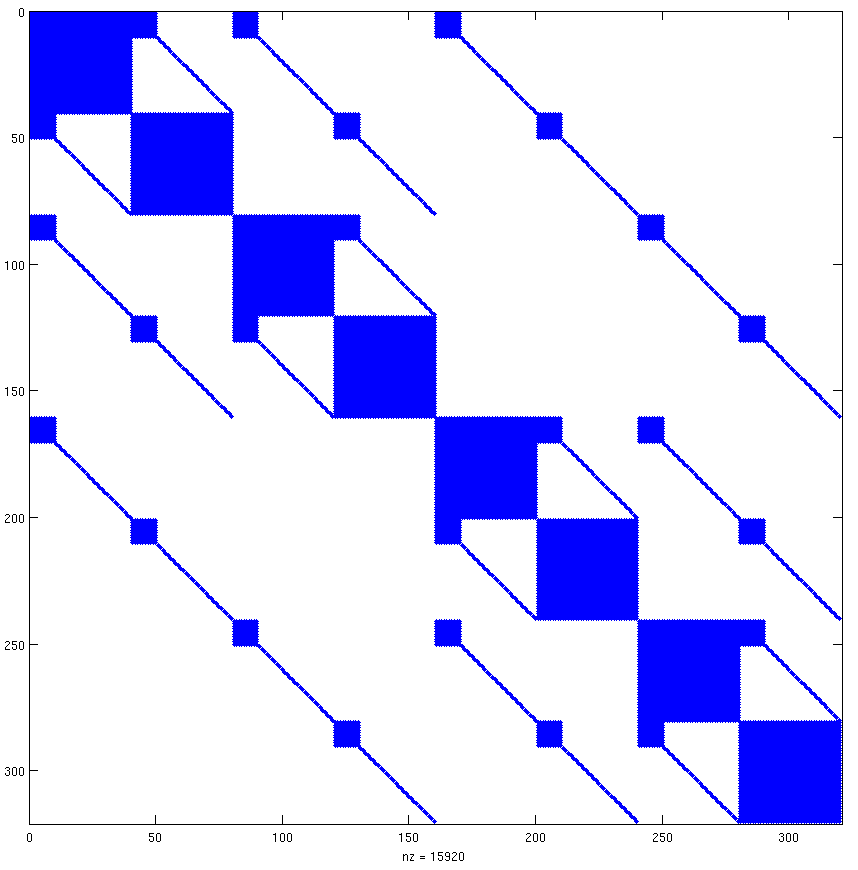
\includegraphics[width=3.3in]{chapters/spn_equations/group10us.png}
  \end{center}
  \caption{\textbf{Sparsity pattern for 10-group $SP_7$ discretization
      with downscatter and upscatter.} \textit{A $2\times 2 \times 2$ element
      mesh was used to show detail of the blocks formed by the
      discretization.}}
  \label{fig:group10us}
\end{figure}

We note a few key features of the sparsity plots. The first is that
for multigroup problems without full upscatter and downscatter
(i.e. Figure~\ref{fig:group10ds}), the resulting matrix is asymmetric
and therefore a linear solver that can handle asymmetric linear
systems is required. Nearly all problems of interest will not have
full upscattering or downscattering. Second we note the largely
diagonal character of these systems, although the blocks from
Eq~(\ref{eq:A_block_matrix}) are readily apparent with a block size of
$N_g\times(N+1)/2$.

Based on this both block and diagonally dominant structure for
matrices formed by the general multigroup $SP_N$ equations, we choose
\textit{block Jacobi} preconditioning as a left preconditioner for the
system. Block Jacobi preconditioning extracts the diagonal block
elements of the matrix to use as the preconditioner as shown on the
left side of Figure~\ref{fig:block_jacobi_ex}. Shown on the right side
of Figure~\ref{fig:block_jacobi_ex}, inversion of the preconditioner
is trivial with each diagonal block inverted separately.

\begin{figure}[t!]
  \begin{center}
    \scalebox{1.6}{
    \input{chapters/spn_equations/block_jacobi.pdftex_t} }
  \end{center}
  \caption{\textbf{Block Jacobi preconditioning strategy used for the
      $SP_N$ equations.} \textit{Left: The preconditioner is formed by
      the diagonal blocks of the matrix. Right: Inversion of the
      preconditioner is trivial and decoupled by block.}}
  \label{fig:block_jacobi_ex}
\end{figure}

For high performance implementations block Jacobi preconditioning has
several attractive properties. First, the blocks in the transport
operator come from the energy/angle discretization of the transport
equation as given by Eq~(\ref{eq:A_block_matrix}). Each block on the
diagonal is bound to a mesh element in the system (note there are 8
blocks on the diagonal in each of the sparsity patterns with a mesh of
$2 \times 2 \times 2$) and therefore we expect the matrix elements
forming the block to be entirely local in domain decomposed
calculations. Second, these blocks are typically dense and nearly
lower triangular for many transport problems meaning that established
dense matrix methods can be used for fast inversion.

\subsection{Block Jacobi Preconditioned Results}
\label{subsec:jacobi_prec_assembly_calc}
A single energy group problem was first computed with $SP_1$
discretization, effectively giving the one-speed neutron diffusion
system for the fuel assembly resulting in 20,088 degrees of freedom in
the problem. Figure~\ref{fig:block_jacobi_res_mcsa} gives the residual
infinity norm as a function of iteration for the MCSA linear solve in
the first eigenvalue iteration using 25,000 stochastic histories at
every iteration for the adjoint Neumann-Ulam solve.
\begin{figure}[t!]
  \begin{center}
    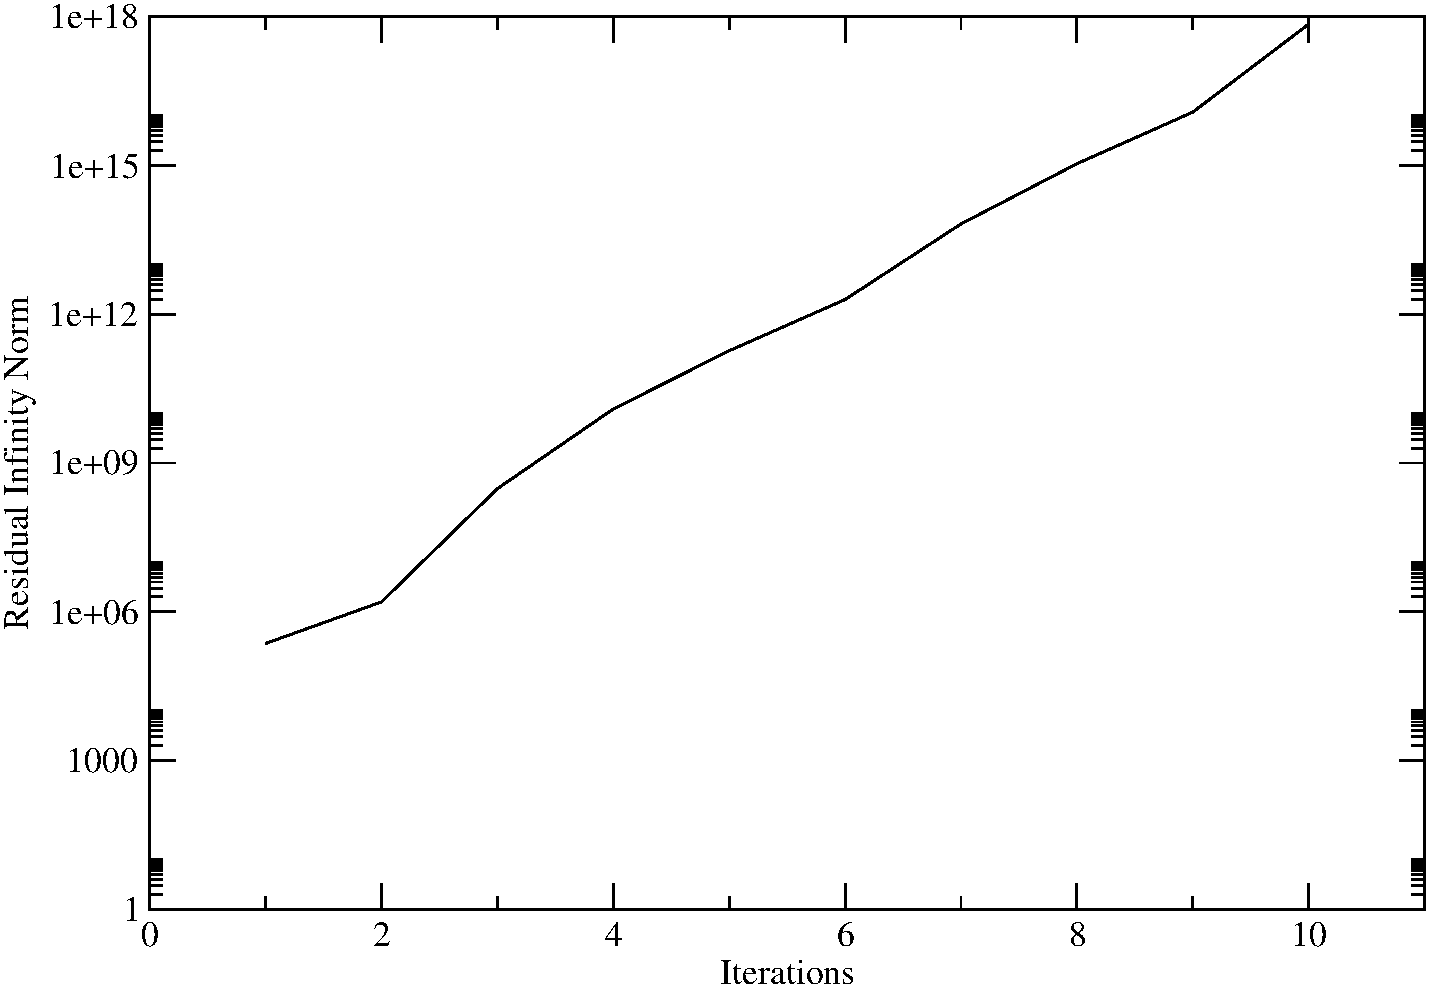
\includegraphics[width=5in]{chapters/spn_equations/block_jacobi_res.pdf}
  \end{center}
  \caption{\textbf{Residual infinity norm vs. iteration for the block
      Jacobi preconditioned MCSA solve during the first eigenvalue
      iteration of the 1-group $17 \times 17$ fuel assembly problem.}
    \textit{Convergence was not achieved with the block Jacobi
      preconditioned method.}}
  \label{fig:block_jacobi_res_mcsa}
\end{figure}
Convergence was not achieved as noted by the rapid rise in the
residual over a few iterations. Based on the spectral radius
computations performed, these results are not in line with
expectations for this problem. Additional computations performed with
\sn{1}{6} histories per iteration exhibited the same divergent
behavior at a significant computational cost and compute time. To
investigate further, a block Jacobi preconditioned Richardson
iteration was used to solve the same
problem. Figure~\ref{fig:block_jacobi_res_richardson} gives the
residual infinity norm as a function of iteration for the Richardson
linear solve in the first eigenvalue iteration.
\begin{figure}[t!]
  \begin{center}
    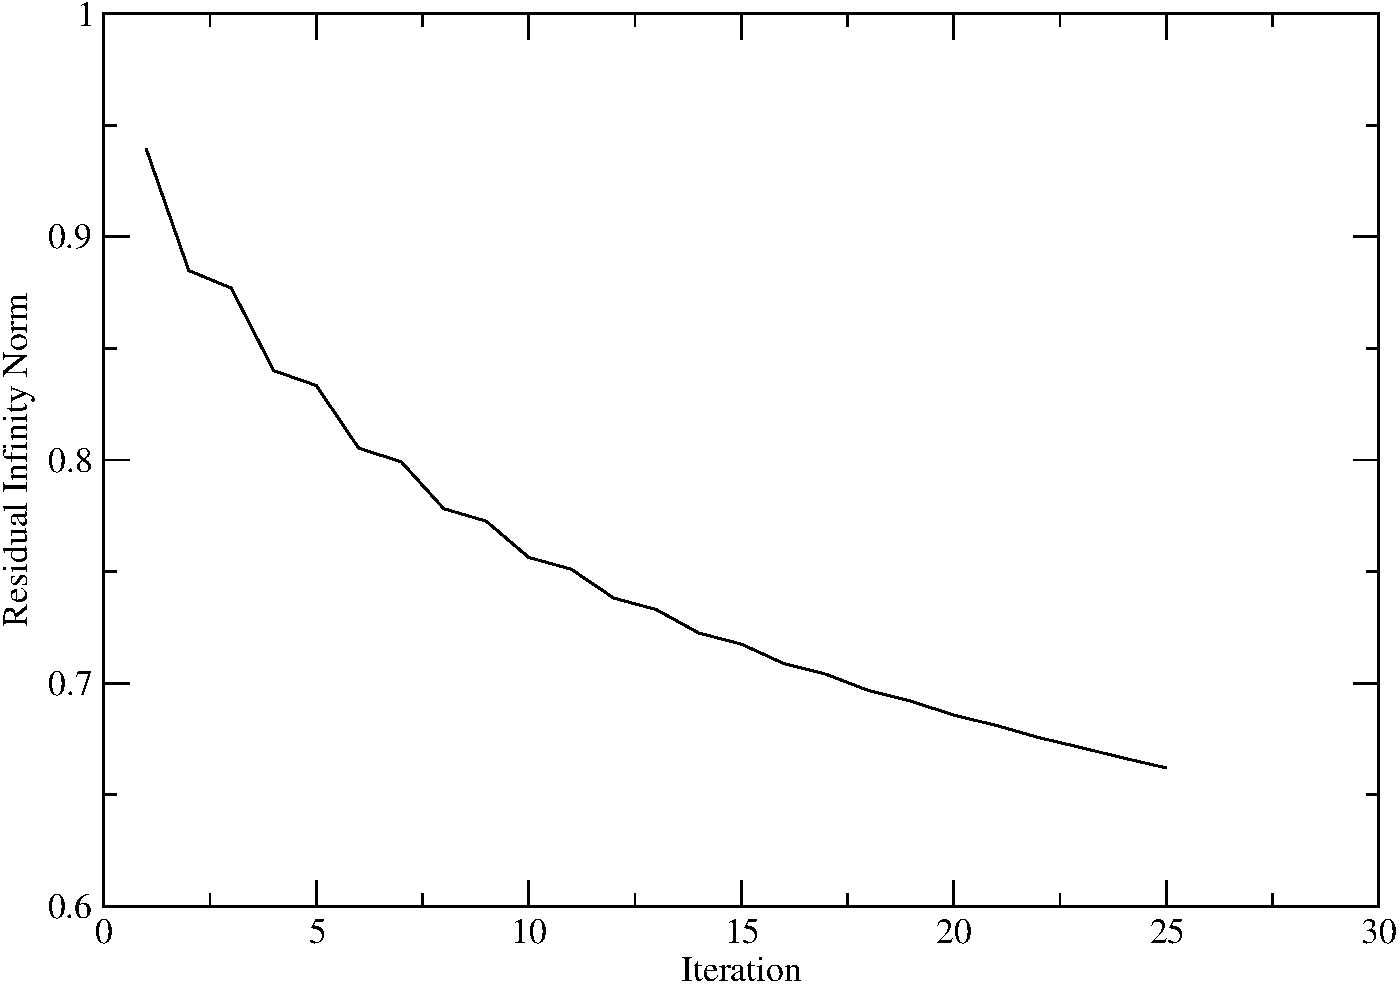
\includegraphics[width=5in]{chapters/spn_equations/block_jacobi_rich_res.pdf}
  \end{center}
  \caption{\textbf{Residual infinity norm vs. iteration for the block
      Jacobi preconditioned Richardson solve during the first
      eigenvalue iteration of the 1-group $17 \times 17$ fuel assembly
      problem.} \textit{A spectral radius near 1 was observed for the
      iteration matrix.}}
  \label{fig:block_jacobi_res_richardson}
\end{figure}
Poor convergence is observed for the Richardson iteration, however,
convergence is achieved meaning that the preliminary eigenvalue
criteria needed to satisfy MCSA convergence has also been met. The
number of iterations required for the Richardson iteration to converge
will give an approximation for the spectral radius via
Eq~(\ref{eq:linear_k_iter_norm3}). With 7291 iterations required to
converge to a tolerance of $\sn{1}{-6}$, $\rho(\mathbf{H}) \approx
0.998$, nearing the limits of MCSA applicability and well beyond the
spectral radii generated in the initial spectral analysis.

Based on these results, it then appears that even if the simple
criteria of a spectral radius of less than one is met and the
Richardson iteration will converge with the same preconditioning, MCSA
still may not converge. We then expect the issue to reside with the
Neumann-Ulam solve providing the correction as the Richardson
iteration is known to provide the correct result. Furthermore, the
fact that the spectral radius is less than one means that the
stochastic histories in the block Jacobi preconditioned Neumann-Ulam
method are eventually being terminated by the weight cutoff as no
artificial absorption was used for these preliminary
calculations. Based on this, the correction being generated by the
Neumann-Ulam solve is the component of MCSA causing a divergent
solution which we study next.

\subsection{MCSA Breakdown}
\label{subsec:mcsa_break_down}
For the fuel assembly problem, the initial block Jacobi preconditioned
calculations used a one-speed $SP_1$ discretization, effectively
giving a diffusion system. To study the breakdown of MCSA at iteration
matrix spectral radii near one, we will use the simpler homogeneous
2-dimensional one-speed neutron diffusion system presented in
Appendix~\ref{chap:diffusion_problem} to isolate this behavior. In
this system, we can vary the cross sections while maintaining a fixed
grid in order to achieve varying spectral radii. For these studies, we
neglect fission as MCSA behavior is dictated by the transport operator
$\mathbf{M}$ in an eigenvalue scheme with the fission matrix used to
generate a fixed source.

For each solver and estimator combination, the spectral radius of the
iteration matrix generated by the diffusion problem was varied by
changing the absorption cross section from 0.25 to 100 while fixing
the grid size at $100 \times 100$ with $h = 0.1$ and a fixed
scattering cross section of unity. For each parameter variation, a
minimum of one stochastic history per degree of freedom (DOF) in the
problem was used to compute the Monte Carlo correction. If the solver
could not converge in less than 100 iterations, the number of
histories was increased by increments of 5,000 until convergence was
achieved in less than 100 iterations. The number of iterations
required to converge MCSA and the time to converge was recorded as a
means to capture the breakdown.

Figure~\ref{fig:breakdown_iterations} gives the number of iterations
required to converge for the chosen number of histories per iteration
given by Figure~\ref{fig:breakdown_histories} using the adjoint solver
with the collision and expected value estimators and the forward
solver with the collision estimator. For spectral radii less than
0.97, all MCSA problems converged with 1 history per DOF (10,000 for
this problem) with the number of iterations required to converge
increasing as a function of spectral radius. Near a spectral radius of
0.97, the number of histories required to converge MCSA in less than
100 iterations takes a dramatic rise that exhibits neither exponential
nor power law behavior. As the spectral radius approaches 1, the
number of histories required becomes significant and effectively
impractical to compute. Even with this simple diffusion problem, the
behavior is consistent with that observed for the fuel assembly
problem with $SP_1$ discretization. In that case, we estimated a
spectral radius of $\approx 0.998$, larger than any of the spectral
radii that could be computed within even 90 minutes of compute time
for this simple two dimensional problem. For that problem, even
1,000,000 histories ($\approx 50$ per DOF) was not enough to provide
convergence. Even if single solve times of an hour can be tolerated,
dozens of solves are typically required to compute the multiplication
factor and flux spectrum within the $SP_N$ eigenvalue scheme for more
difficult problems like the fuel assembly, making the method unusable.
\begin{figure}[t!]
  \begin{center}
    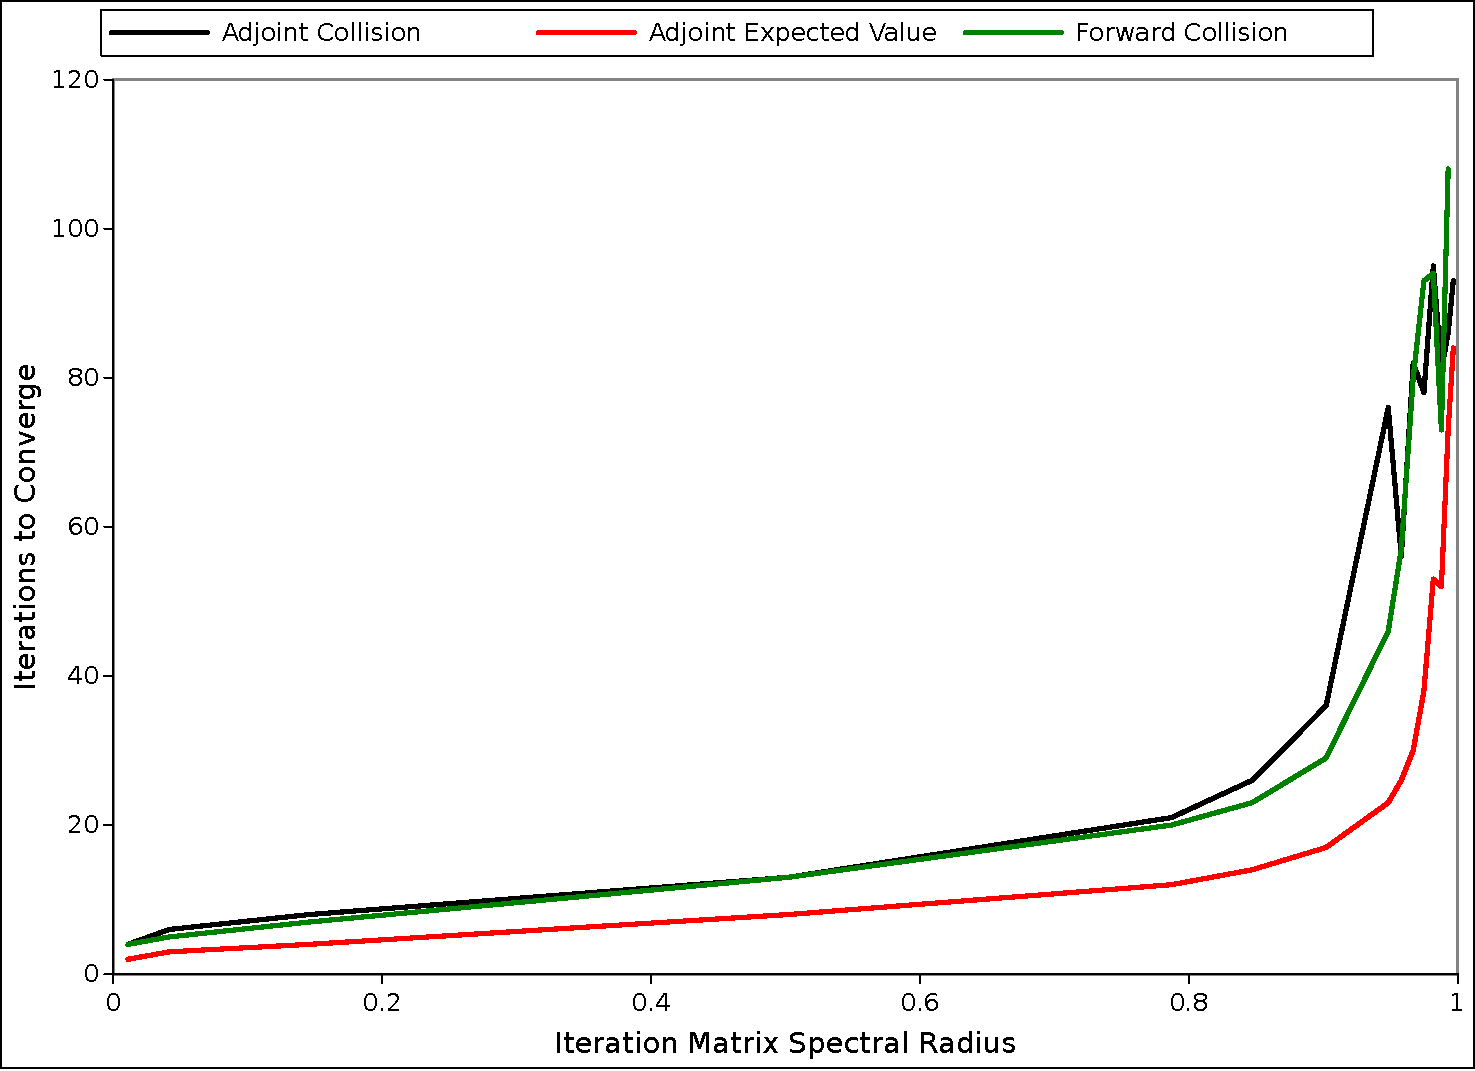
\includegraphics[width=5.75in]{chapters/spn_equations/breakdown_iterations.pdf}
  \end{center}
  \caption{\textbf{Iterations required to converge as a function of
      spectral radius for the neutron diffusion problem.} \textit{The
      number of histories was increased to achieve convergence in less
      than 100 iterations. At least 10,000 histories were used for
      each calculation.}}
  \label{fig:breakdown_iterations}
\end{figure}
\begin{figure}[t!]
  \begin{center}
    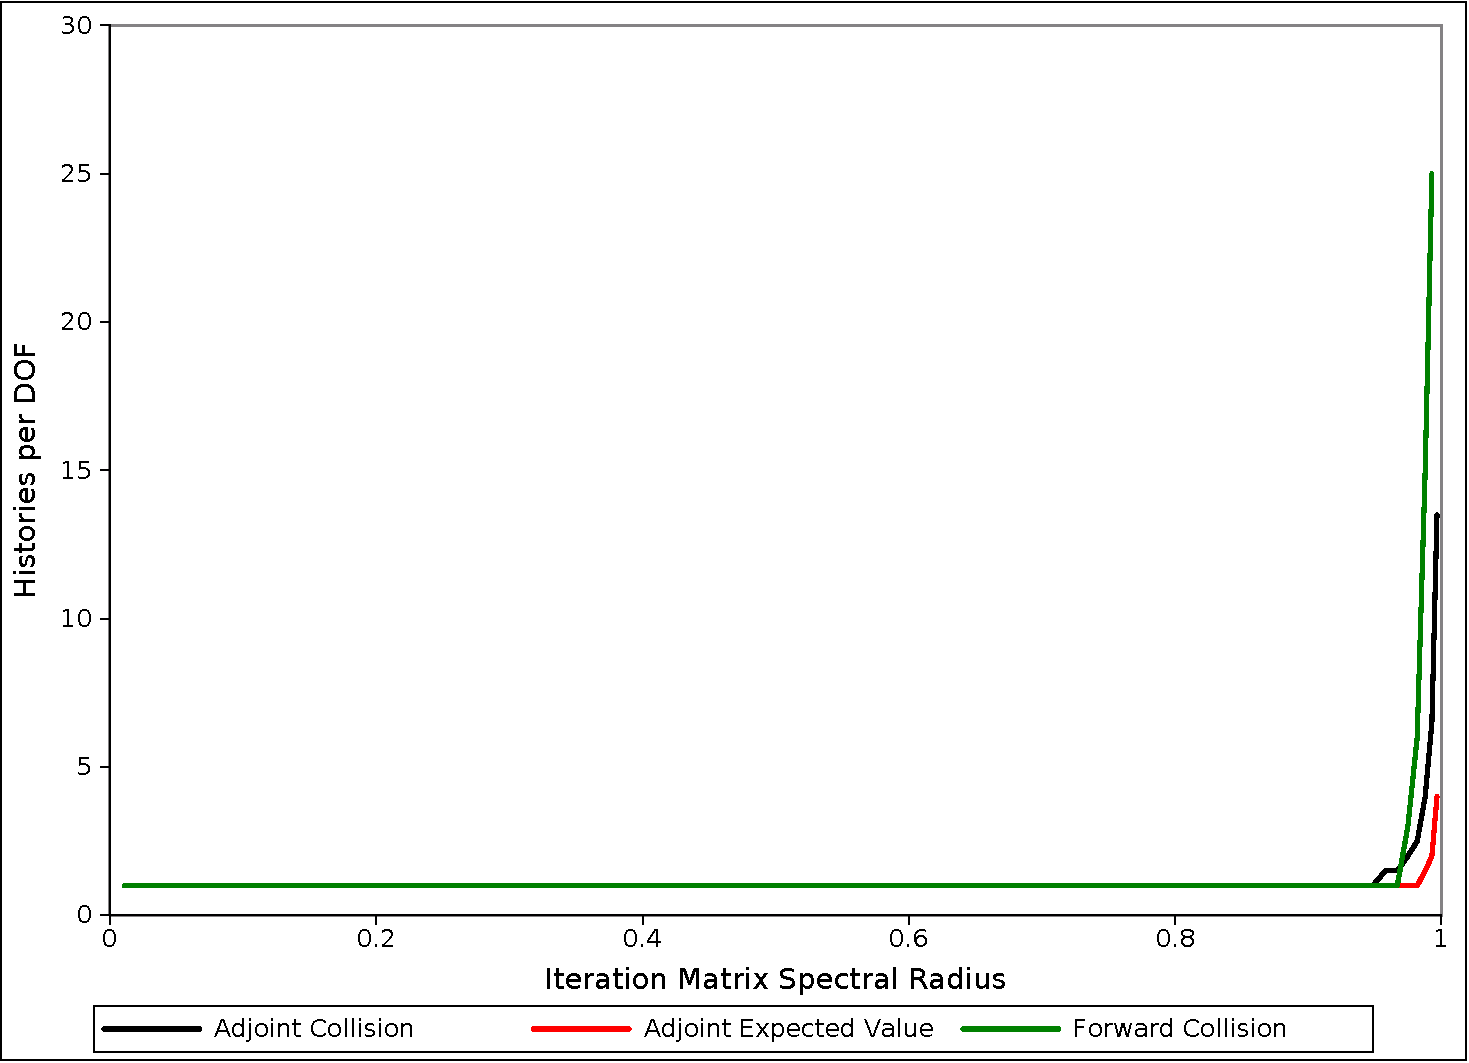
\includegraphics[width=5.75in]{chapters/spn_equations/breakdown_histories.pdf}
  \end{center}
  \caption{\textbf{Histories per DOF required to converge as a
      function of spectral radius for the neutron diffusion problem.}
    \textit{The number of histories was increased to achieve
      convergence in less than 100 iterations. At least 10,000
      histories were used for each calculation with 10,000 DOFs in the
      problem.}}
  \label{fig:breakdown_histories}
\end{figure}

In addition to the significantly larger number of histories required
to achieve convergence for ill-conditioned problems another penalty is
paid due to histories that take longer to
compute. Figure~\ref{fig:breakdown_time} gives the CPU time in seconds
required to compute a single random walk averaged over the entire set
of histories run in the calculation over all iterations. As the
spectral radius increases (correlating to a higher ratio of scattering
in the system) the random walk lengths increase, using more CPU time
to finish the computation. Compared to spectral radii of 0.5, larger
spectral radii over 0.97 have histories that require two orders of
magnitude more computation time. This significant increase in
computation time per history coupled with the significant increase in
the number of histories required to converge is evidence that for
problems with spectral radii above $\approx 0.97$, using MCSA to solve
any problems of interest is entirely ineffective and not practical. At
iteration matrix spectral radii this large, using significant numbers
of stochastic histories in the Monte Carlo solve is not enough to
reduce the stochastic uncertainty in the correction, causing the MCSA
sequence to diverge instead of accelerating convergence. We therefore
require a more expansive set of preconditioning techniques to move the
eigenvalue spectrum of the $SP_N$ problem into a regime in which MCSA
is more applicable and in which performance is improved.
\begin{figure}[t!]
  \begin{center}
    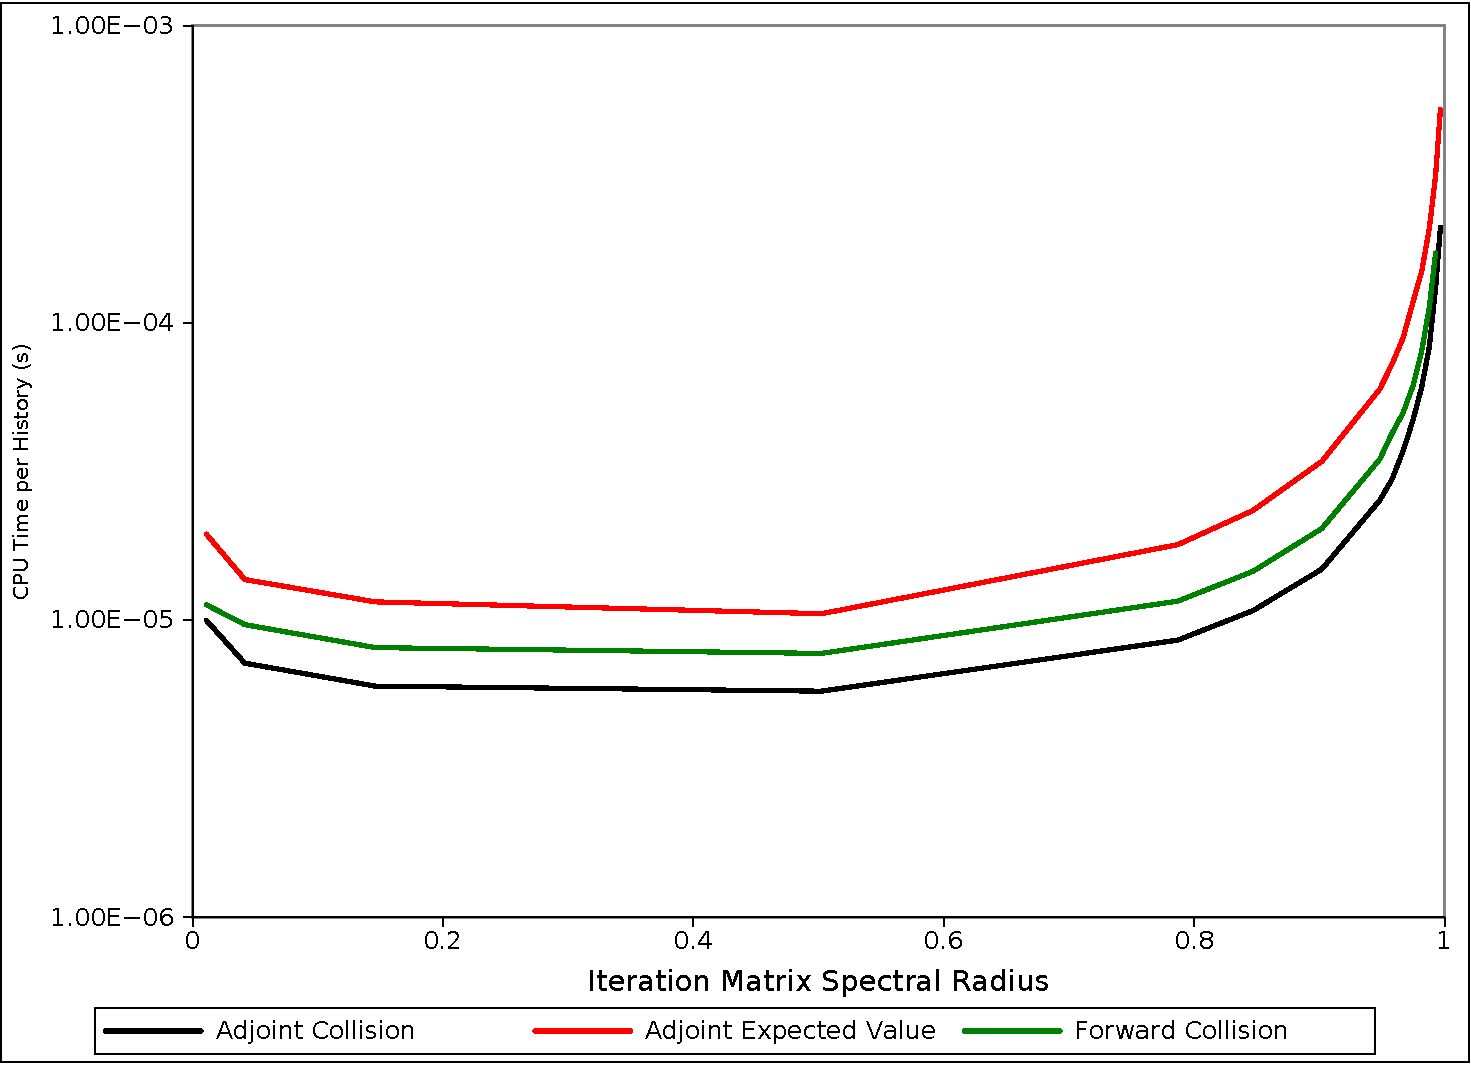
\includegraphics[width=5.75in]{chapters/spn_equations/breakdown_time.pdf}
  \end{center}
  \caption{\textbf{CPU time per history as a function of spectral
      radius for the neutron diffusion problem.} \textit{As the
      spectral radius grows, so do the length of the random
      walks. Longer random walks require more CPU time to compute.}}
  \label{fig:breakdown_time}
\end{figure}

\clearpage

%%---------------------------------------------------------------------------%%
\section{Advanced Preconditioning Strategies}
\label{subsec:spn_advanced_preconditioning}
For the fuel assembly criticality problem presented in the previous
section, the spectral radius was near one using Jacobi preconditioning
and in a regime in which MCSA breakdown is observed. In this regime
the number of stochastic histories required to converge MCSA increases
rapidly and the resulting poor performance is compounded by those
histories being increasingly expensive to compute. To overcome this
difficulty, advanced preconditioning strategies for the $SP_N$ problem
are required beyond simple Jacobi methods that can reduce the spectral
radius into a region of better MCSA performance. Two modern algebraic
preconditioning strategies, ILUT and SPAINV, will be presented here
and used within the explicit preconditioning framework given by
Eq~(\ref{eq:left_right_mcsa}). Data showing their effects on MCSA
solutions of the fuel assembly criticality problem will be provided.

\subsection{ILUT Preconditioning}
\label{subsec:spn_ilut_preconditioning}
ILUT preconditioning is chosen first due to its applicability to
problems that have a dominating elliptic component such as the fuel
assembly problem or other problems with a high scattering to
absorption ratio. As with MCSA, the algebraic formulation of ILUT
requires the physics operator to be fully formed and is therefore
easily incorporated into our solution sequence. 

Incomplete lower-upper (ILU) factorizations of the linear operator can
be used as a simple mechanism to form an approximate inverse of a
preconditioner. To build the factorization, the sparse upper and lower
triangular factors, $\mathbf{L}$ and $\mathbf{U}$, are computed such
that the residual matrix formed by the factorization
\cite{saad_iterative_2003}:
\begin{equation}
  \mathbf{R} = \mathbf{L} \mathbf{U} - \mathbf{A} \:,
  \label{eq:ilu_residual_matrix}
\end{equation}
has a specified sparsity pattern and element magnitude. When a
magnitude threshold is used, elements generated in the factors below
that magnitude are dropped, resulting in ILU threshold (ILUT)
preconditioning. The sparsity pattern in this case is determined from
the input matrix to be preconditioned and the number of elements
maintained in the factor is specified by a fill level parameter. A
fill level of 1 will generate the same number of elements as the
sparsity pattern of the input matrix while a fill level of 2 will
contain twice as many elements in the factorization, resulting in a
better representation of the true LU factorization. The inverse of the
lower and upper triangular factors may then be easily inverted by
means of simple elimination procedure to produce the
preconditioner. For MCSA, $\mathbf{L}^{-1}$ will be used on the left
and $\mathbf{U}^{-1}$ on the right to precondition the system.

For the explicit preconditioning scheme presented in
Eq~(\ref{eq:left_right_mcsa}), the fully inverted operator must be
generated in order to build the set of probabilities and weights
required for Monte Carlo sampling. Therefore, for a linear system of
size $N$, $N$ triangular solves will be required in order to extract
the inverse matrices from production ILU implementations. In addition,
parallel implementations typically generate lower and upper factors
that are only triangular locally, providing an easily parallelizable
mechanism to generate the action of the preconditioner inverse. A
consequence of this choice for parallel scalability is a degradation
of the preconditioning quality as the size of the parallel system is
increased. For serial computations, the triangular factorization is
potentially exact depending on the parameters chosen while at
thousands of parallel tasks, the global triangular factors differ
significantly from the true factorization. As a result, more
iterations are required at higher levels of parallelism to converge
the system and will ultimately degrade overall scalability of the
system with respect to total wall time to converge.

MCSA preconditioned with ILUT was used to solve the fuel assembly
problem presented in the previous section for a 1-group $SP_1$
discretization. Unlike the Jacobi preconditioned strategy, convergence
was achieved with ILUT preconditioning. To study convergence
sensitivity to ILUT parameters, the fill level and drop tolerance were
parametrically varied with the number of iterations to converge an
eigenvalue iteration for the fuel assembly problem recorded along with
the maximum number of non-zero entries observed in all matrix rows for
the left/right preconditioned composite linear operator. To provide
some sparsity to the factorization, the ILUT drop tolerance was used
to drop elements in the extracted inverse triangular factors. For each
calculation, the number of iterations required to converge reported
was for a single eigenvalue iteration with \sn{3}{4} histories at each
MCSA iteration to compute the Monte Carlo correction using the adjoint
collision estimator. All ILUT calculations reported here were
performed on a single CPU and therefore this data does not take into
account the aforementioned effects of parallel decomposition on the
quality of the ILUT preconditioning.

Figure~\ref{fig:ilut_iterations} gives the number of iterations to
converge the fixed source problem to a tolerance of \sn{1}{8}. As
expected, the higher the fill level chosen for the ILUT factorization,
the fewer iterations are required to converge the problem with only 9
MCSA iterations were required to converge the problem for the fill
level of 3 and drop tolerance of \sn{1}{-5} case. For higher levels of
fill, the iterations needed to converge were not as sensitive,
signaling that a larger drop tolerance can perhaps be used without a
significant degradation in iterative performance. At smaller fill
levels, the sensitivity to the ILUT drop tolerance is more
significant. For all fill levels used, convergence was not achieved
for the fuel assembly problem with a drop tolerance larger than
\sn{1}{-3}.
\begin{figure}[t!]
  \begin{center}
    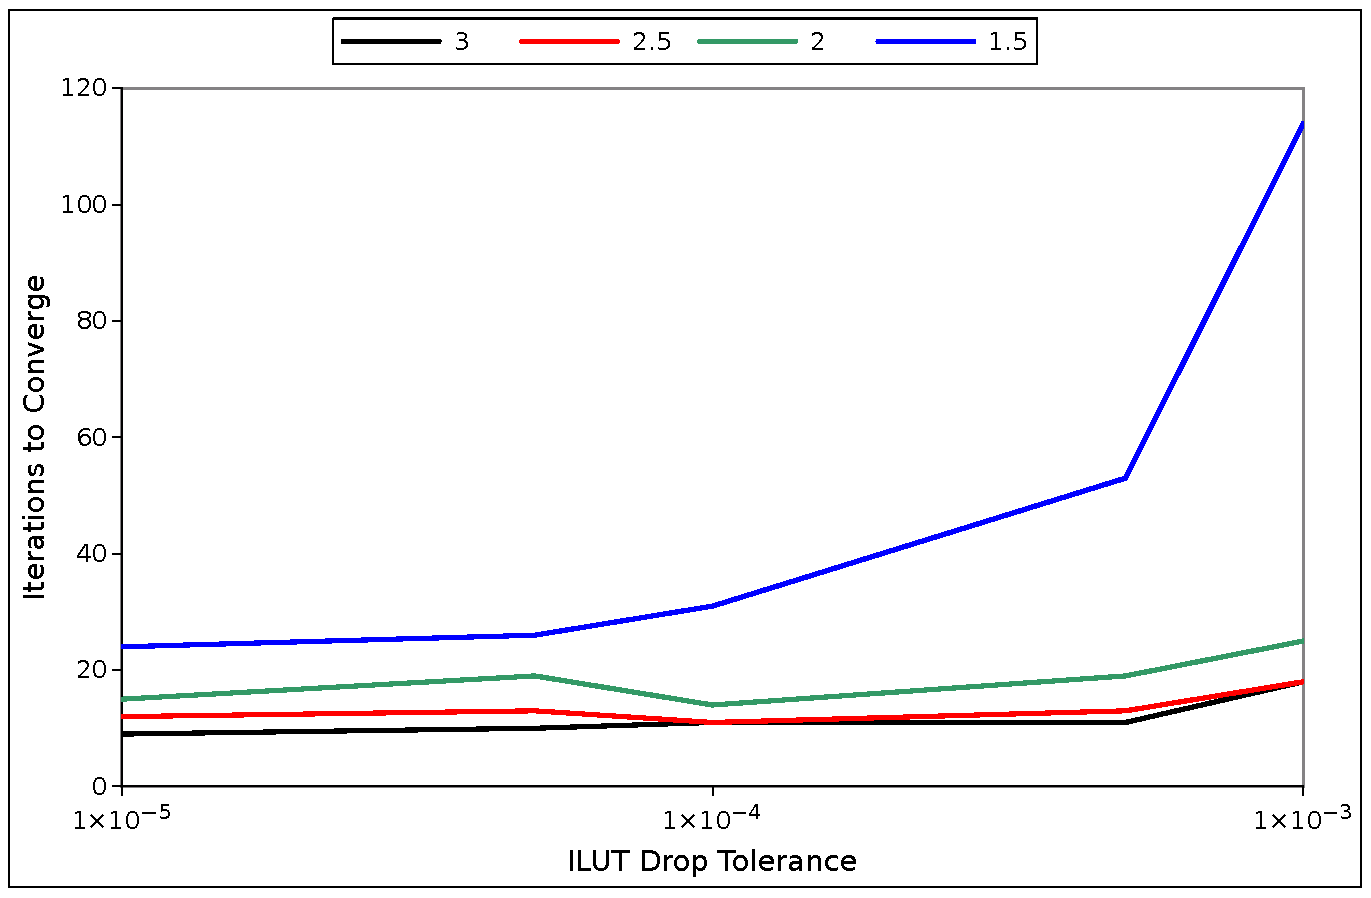
\includegraphics[width=4.25in]{chapters/spn_equations/ilut_iterations.pdf}
  \end{center}
  \caption{\textbf{Number of MCSA iterations required to converge an
      eigenvalue iteration for the fuel assembly problem with ILUT
      preconditioning as a function of ILUT drop tolerance.}
    \textit{Each colored curve represents the iteration behavior for a
      different ILUT fill level. Fill levels of 1.5, 2.0, 2.5, and 3.0
      were used.}}
  \label{fig:ilut_iterations}
\end{figure}

Unfortunately, gaining convergence (and excellent iterative
performance) with MCSA for the $SP_N$ fuel assembly problem comes at
an immediate cost. Figure~\ref{fig:ilut_size} gives the maximum number
of non-zero entries in the composite linear operator generated by
preconditioning as a function ILUT drop tolerance for varying values
of fill level. For the 1-group $SP_1$ discretization, the original
linear operator will contain only a maximum of 7 non-zero entries per
row in the system. As observed in Figure~\ref{fig:ilut_size},
performing the explicit preconditioning yields composite linear
operators with $O(1,000)$ elements in a row for all combinations of
fill level and drop tolerance, over 10\% of the total row size for
this particular problem. This large number of row entries, observed
for a significant fraction of rows in the system, creates several
problems. First, sparsity is completely destroyed with each state in
the system now coupled to over 10\% of the total states in the system
through the composite iteration matrix. This means that Monte Carlo
sampling tables will be large, requiring significant memory to store
them and a substantial overhead in the sampling procedure during
transport. Second, the matrix-matrix multiply operations required to
build the composite operator see significant performance losses due to
the amount of data that must be handled. In parallel, losing sparsity
severely inhibits performance where now parallel operations require
communications among orders of magnitude more processors for
nearest-neighbor type algorithms.

\begin{figure}[t!]
  \begin{center}
    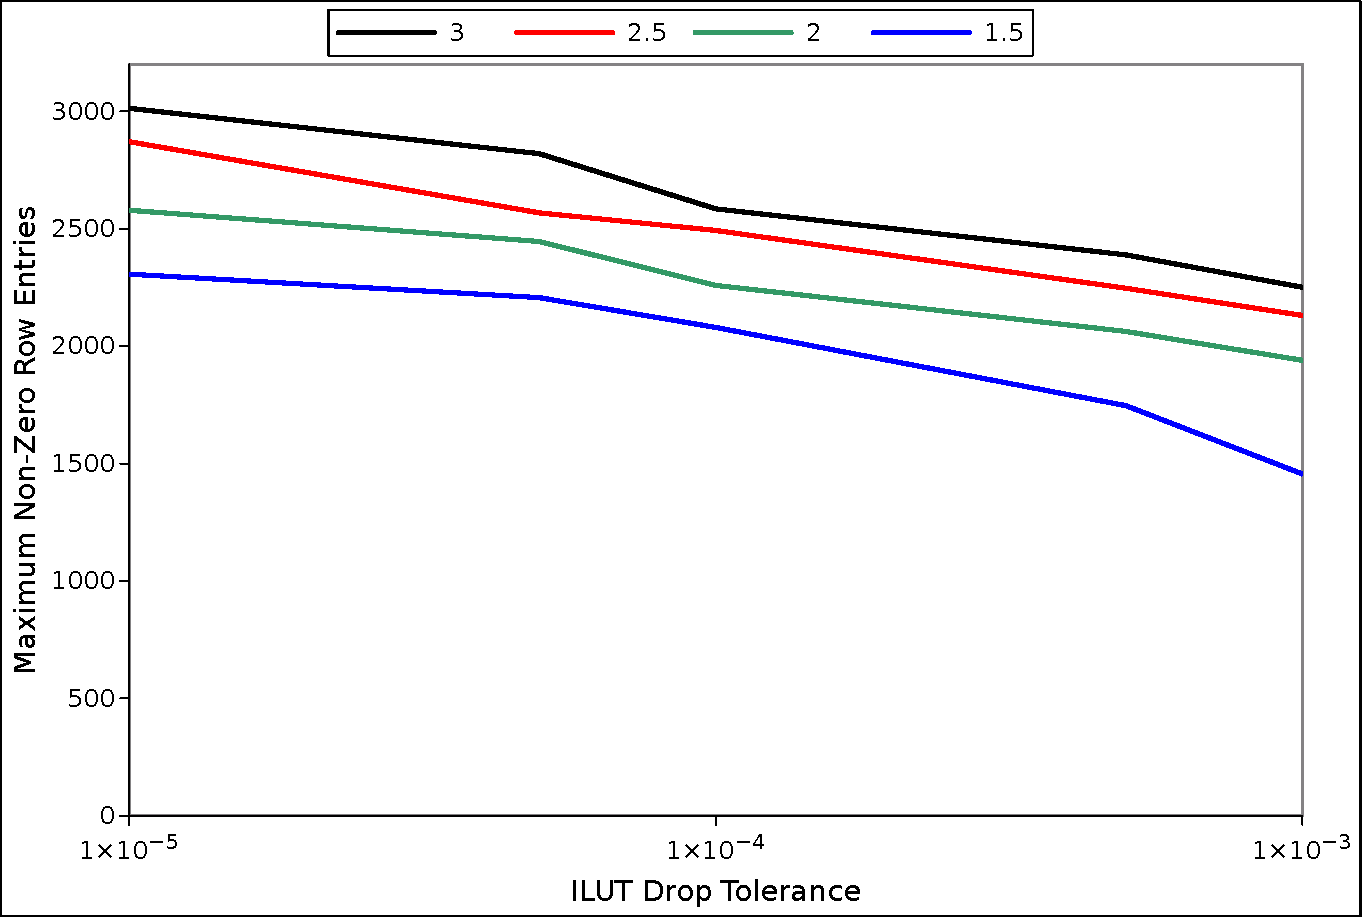
\includegraphics[width=4.25in]{chapters/spn_equations/ilut_size.pdf}
  \end{center}
  \caption{\textbf{Maximum number of non-zero entries observed for all
      rows in the composite linear operator for the fuel assembly
      problem with ILUT preconditioning given as a function of ILUT
      drop tolerance.} \textit{Each colored curve represents the row
      size for a different ILUT fill level. Fill levels of 1.5, 2.0,
      2.5, and 3.0 were used.}}
  \label{fig:ilut_size}
\end{figure}

As a means to assess the quality of the preconditioning, a simple
metric is developed to address these concerns and allow comparison to
future developments. For our studies, our core performance metric will
be iterative performance with the minimum number of MCSA iterations
required to converge the problem desired. For Monte Carlo
calculations, this improved performance is balanced by the creation of
a dense composite system and we seek to reduce the number of non-zero
entries to a minimum value in order to lower the amount of coupling
among states in the system and reduce the amount of memory used
along with the potential latency overhead. Given these two objectives,
the following metric is proposed:
\begin{equation}
  \text{Quality Metric} = (\text{\# iterations}) \times (\text{maximum
    \# non-zero values})\:,
\end{equation}
where the highest quality preconditioning is one that minimizes this
metric. For the ILUT preconditioned data provided,
Figure~\ref{fig:ilut_quality} provides the computed metric as a
function of ILUT drop tolerance for each fill level used. In general,
the metric is similar to the data observed for the number of
iterations required to converge as the non-zero row entries changed by
a smaller fraction over drop tolerances tested. For higher levels of
fill, the quality metric is observed to be relatively insensitive to
the drop tolerance as maintaining more entries in the preconditioner
has a stronger impact than filtering small values.

\begin{figure}[t!]
  \begin{center}
    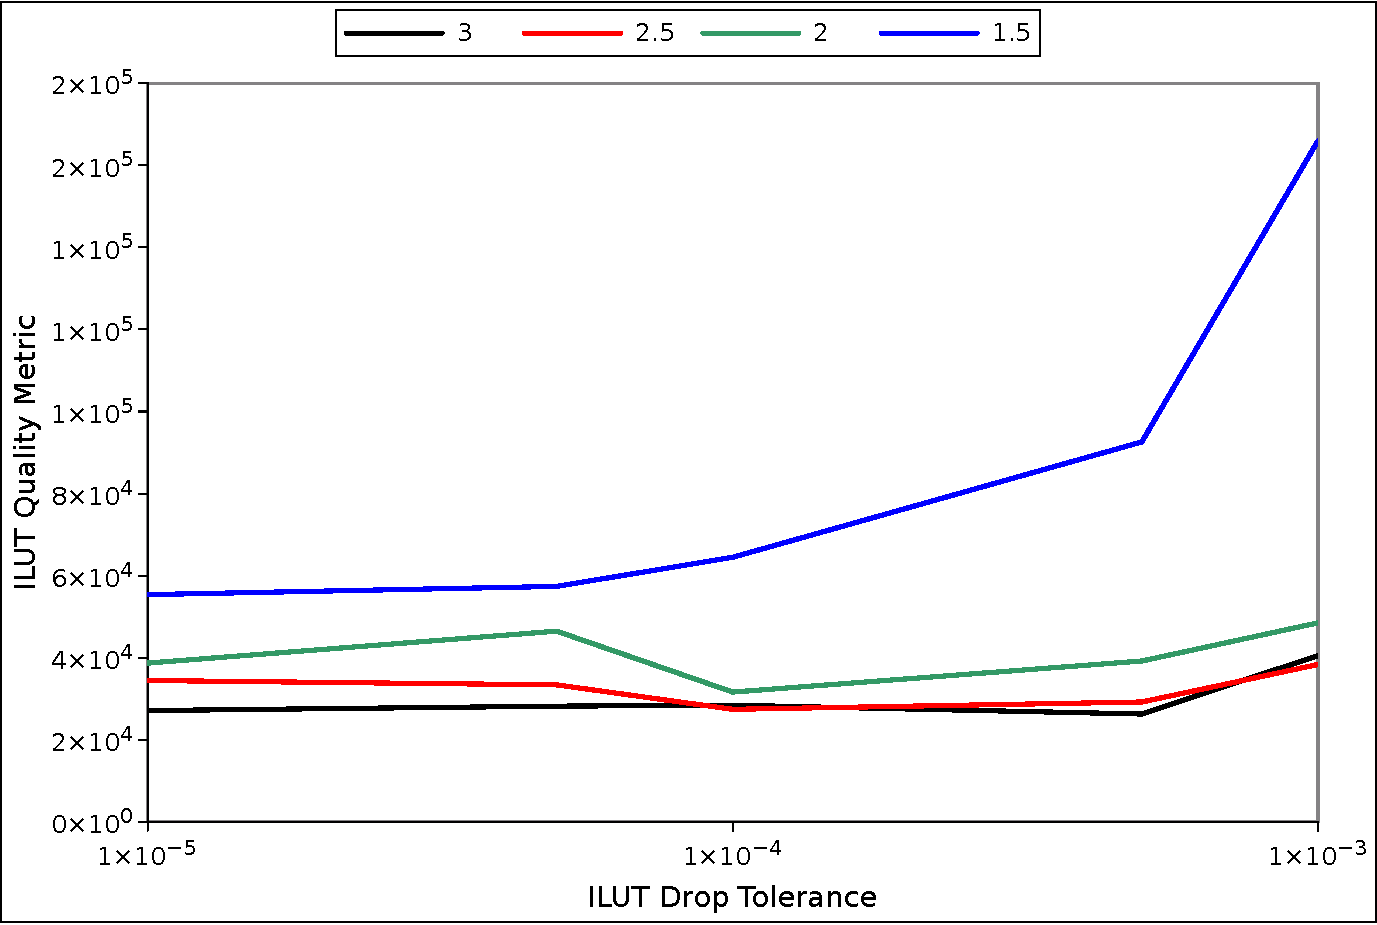
\includegraphics[width=4.25in]{chapters/spn_equations/ilut_quality.pdf}
  \end{center}
  \caption{\textbf{ILUT preconditioning quality metric for the fuel
      assembly problem given as a function of ILUT drop tolerance.}
    \textit{Each colored curve represents the quality metric behavior
      for a different ILUT fill level. Fill levels of 1.5, 2.0, 2.5,
      and 3.0 were used.}}
  \label{fig:ilut_quality}
\end{figure}


\subsection{Sparse Approximate Inverse Preconditioning}
\label{subsec:spn_spainv_preconditioning}
Sparse approximate inverse (SPAINV) preconditioning is chosen next because the true inverse of the preconditioner
is product of the algorithm, avoiding the need for many inverse matrix
applications as required by using ILUT with MCSA. In addition, the
algorithm seeks to maintain the sparsity of the inverse
preconditioner, potentially alleviating some of the dense operator
issues observed with ILUT.

SPAINV produces a sparse approximation of the inverse matrix directly
by minimizing the Frobenius norm of the residual matrix
\cite{saad_iterative_2003}:
\begin{equation}
  || \mathbf{I} - \mathbf{A} \mathbf{M} ||^2_F =
  \sum_{j=1}^N ||\mathbf{e}_j - \mathbf{A} \mathbf{m}_j||^2_2 \:,
  \label{eq:frobenius_norm_min}
\end{equation}
where the inverse preconditioning matrix $\mathbf{M}$ minimizes the
norm on the right and $\mathbf{e}_j$ and $\mathbf{m}_j$ are the
$j^{th}$ columns of the identity and preconditioning matrices
respectively. Here, $\mathbf{M}$ is the actual inverse of the
preconditioner and is formed directly by the algorithm. On the right
hand side of Eq~(\ref{eq:frobenius_norm_min}), the Frobenius norm is
represented as a effective sum of $N$ linear system residual norms. 

A few iterations of a subspace method or other iterative scheme can be
used to effectively solve these systems to a loose tolerance and yield
the columns of the approximate preconditioning matrix. At each
iteration, threshold values are used to eliminate the components of
each $\mathbf{m}_j$ column to maintain the desired level of
sparsity. In addition, a sparsity pattern can be predetermined and
enforced during this process. For the SPAINV implementation used for
this work, the sparsity pattern was defined by levels such that a
level of $N$ for an input operator $\mathbf{A}$ will generate a
preconditioning matrix $\mathbf{M}$ with the same sparsity pattern as
$\mathbf{A}^{N+1}$. By using the norm minimization strategy instead of
a factorization such as ILUT, parallel results are reproduced
regardless of parallel problem size, meaning that a serial computation
will converge in the same number of iterations as a computation with
thousands of cores.

MCSA preconditioned with SPAINV was used to solve the fuel assembly
problem again for a 1-group $SP_1$ discretization. To study
convergence sensitivity to SPAINV parameters, the number of levels in
the sparsity pattern and threshold were parametrically varied with the
number of iterations to converge a single eigenvalue iteration for the
fuel assembly problem recorded along with the maximum number of
non-zero entries observed in all matrix rows for the preconditioned
composite linear operator. For each calculation, the number of
iterations required to converge reported was for a single eigenvalue
iteration with \sn{3}{4} histories at each MCSA iteration to compute
the Monte Carlo correction using the adjoint collision estimator. All
SPAINV calculations reported here were performed on a single CPU.

Figure~\ref{fig:spainv_iterations} gives the number of MCSA iterations
needed to converge the fuel assembly problem and
Figure~\ref{fig:spainv_size} the maximum number of non-zero entries
per row observed in the composite linear operator as a function the
SPAINV threshold. For this analysis, the number of levels in the
sparsity pattern was varied from 3 to 7 with convergence of the fuel
assembly problem not achieved for smaller level values. Compared to
ILUT preconditioning, at higher levels we see comparable iterative
performance with a relative invariance to the threshold value. The
threshold did have a significant effect, however, on the time required
to generate the preconditioner with a threshold of 0.001 over an order
of magnitude slower than a threshold of 0.01 due to the inclusion of a
significant number of extra values in the input operator. In addition
to comparable iterative performance, the sparsity of the composite
operator is greatly improved with nearly an order of magnitude
reduction in number of non-zero entries per row for lower level
values.

\begin{figure}[t!]
  \begin{center}
    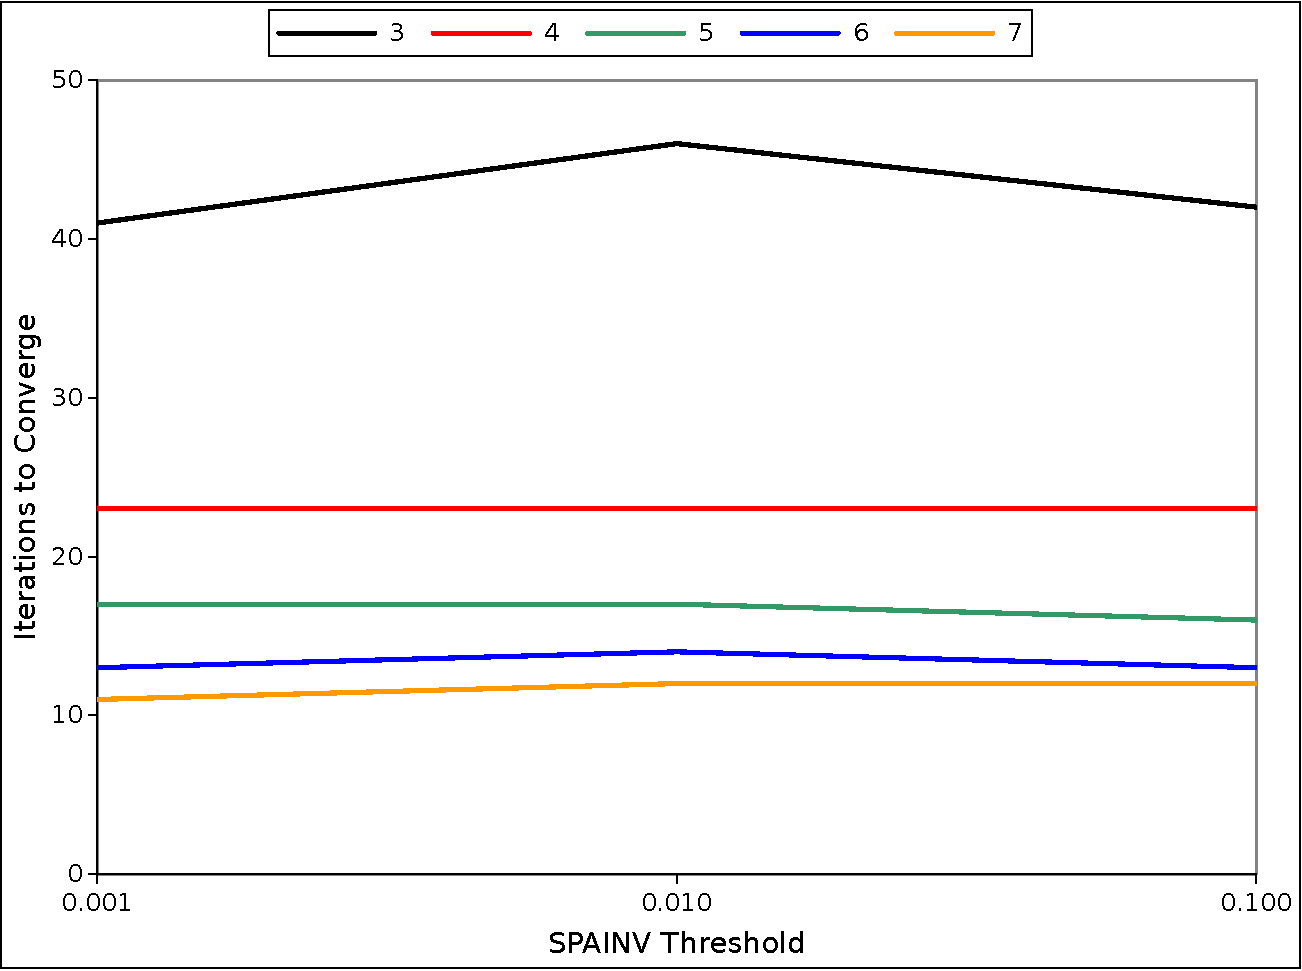
\includegraphics[width=4.25in]{chapters/spn_equations/spainv_iterations.pdf}
  \end{center}
  \caption{\textbf{Number of MCSA iterations required to converge a
      single eigenvalue iteration for the fuel assembly problem with
      SPAINV preconditioning as a function of SPAINV threshold.}
    \textit{Each colored curve represents the iteration behavior for a
      different SPAINV level pattern. Levels of 3, 4, 5, 6, and 7 were
      used.}}
  \label{fig:spainv_iterations}
\end{figure}
\begin{figure}[t!]
  \begin{center}
    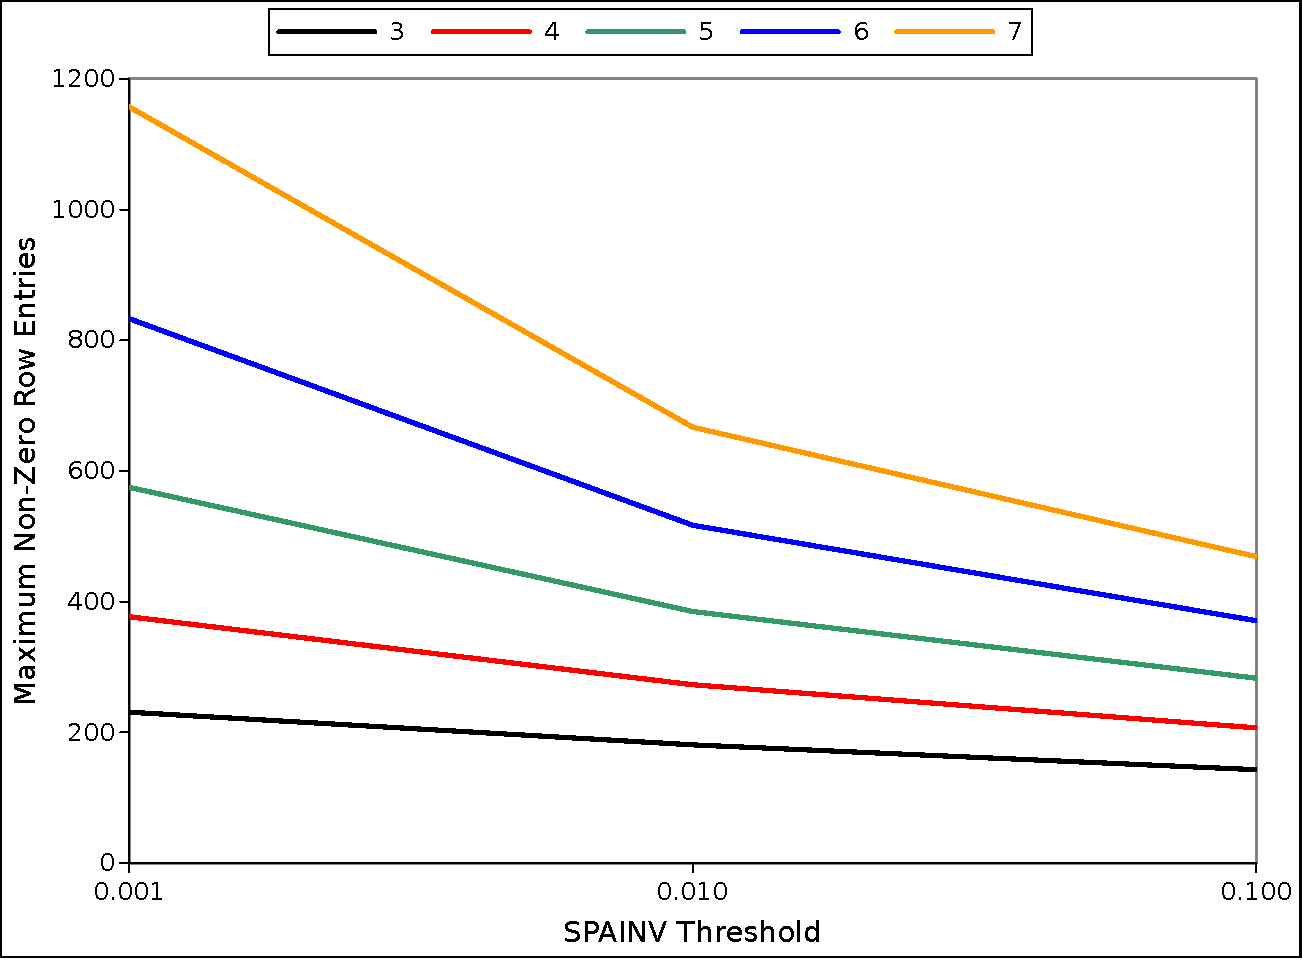
\includegraphics[width=4.25in]{chapters/spn_equations/spainv_size.pdf}
  \end{center}
  \caption{\textbf{Maximum number of non-zero entries observed for all
      rows in the composite linear operator for the fuel assembly
      problem with SPAINV preconditioning given as a function of
      SPAINV threshold.} \textit{Each colored curve represents the row
      size for a different SPAINV level pattern. Levels of 3, 4, 5, 6,
      and 7 were used.}}
  \label{fig:spainv_size}
\end{figure}

Figure~\ref{fig:spainv_quality} gives the quality metric as a function
of the threshold value for each of the sparsity levels computed. Not
only do we see an improved quality metric over ILUT preconditioning
(about an order of magnitude less), but we also note that the ideal
sparsity level is not the largest nor the smallest. In fact, the
largest and smallest levels (3 and 7) performed the worst in terms of
the quality metric with a level of 4 performing the best.

\begin{figure}[t!]
  \begin{center}
    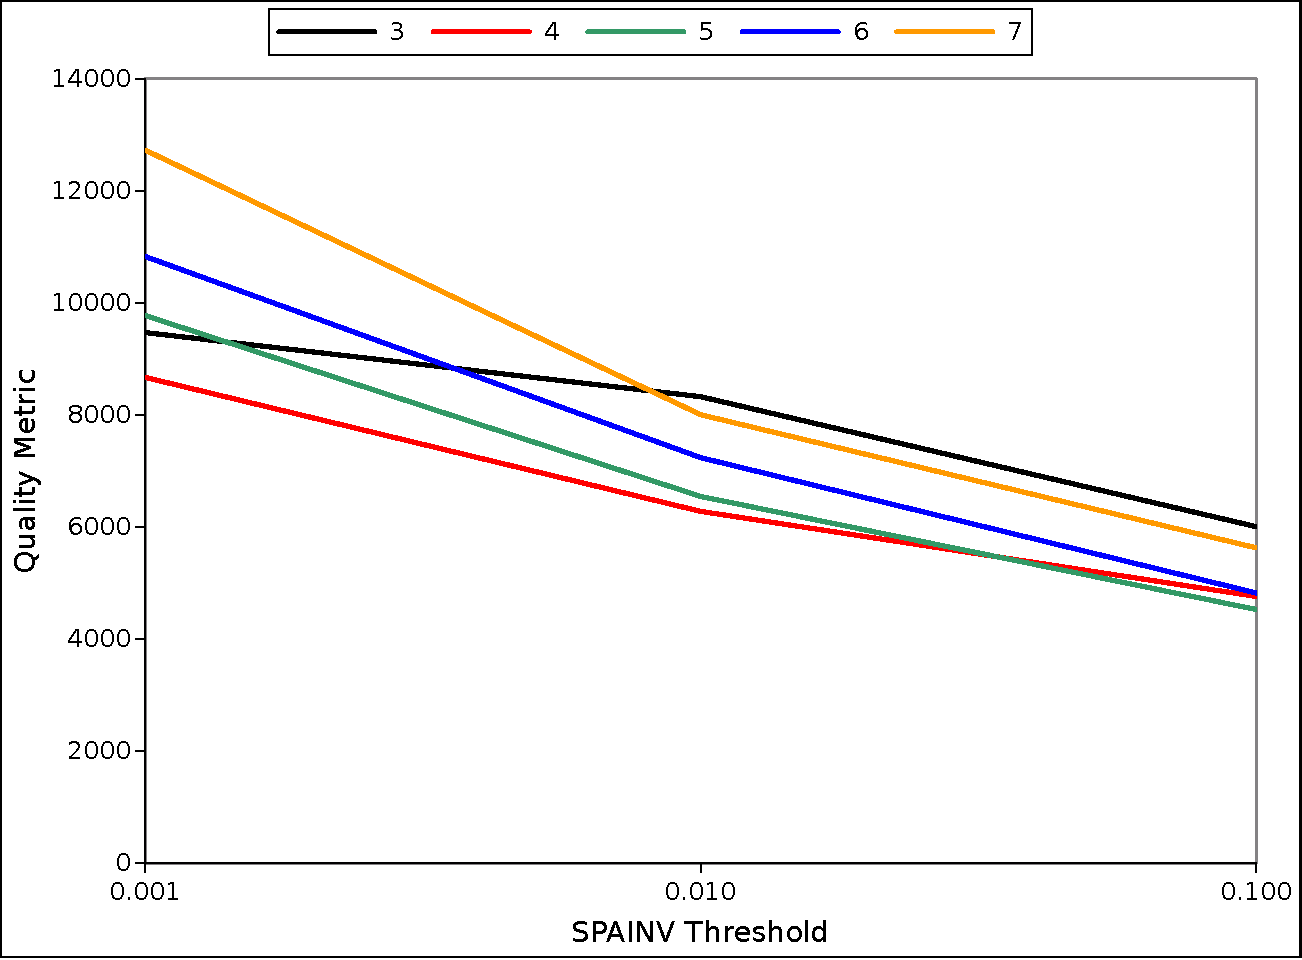
\includegraphics[width=4.25in]{chapters/spn_equations/spainv_quality.pdf}
  \end{center}
  \caption{\textbf{SPAINV preconditioning quality metric for the fuel
      assembly problem given as a function of SPAINV threshold.}
    \textit{Each colored curve represents the quality metric behavior
      for a different SPAINV level pattern. Levels of 3, 4, 5, 6, and
      7 were used.}}
  \label{fig:spainv_quality}
\end{figure}

\clearpage

\subsection{Applying the Reduced Domain Approximation}
\label{subsec:spn_prec_rda}
Although ILUT and SPAINV preconditioning permitted MCSA solutions for
the fuel assembly problem, a primary concern is the number of non-zero
states in each row of the system generated by the explicit
preconditioning strategy. In many cases, orders of magnitude more
matrix elements were generated resulting in poor scalability for
domain decomposed algorithms and overall performance issues for Monte
Carlo. As outlined in \S~\ref{subsec:reduced_domain_approximation},
the reduced domain approximation may be used as a mechanism to
potentially alleviate this problem by filtering elements of the
composite matrix in each row that fall below a certain threshold value
or by maintaining the largest $N$ elements in each row where $N$ is a
designated fill level. In this section, we will apply the reduced
domain approximation to both ILUT and SPAINV preconditioned system to
reduce the density of the composite linear operator to more manageable
levels and study the resulting iterative performance.

For each preconditioner, the parameters that achieved the best quality
metric results from the previous analysis were used. These correspond
to ILUT parameters of a fill level of 5.0 and a drop tolerance of
\sn{1}{-5} and SPAINV parameters of a sparsity level of 4 and a
threshold of 0.1. The reduced domain threshold was set to \sn{1}{-10}
in order to eliminate any exceedingly small values from the matrix
(often this is simply removing non-zero elements within the floating
point tolerance of zero). The reduced domain fill level was then
varied, starting with the largest non-zero entries per row value
observed for each of the preconditioning types in order to assess its
effects relative to the case where no reduced domain approximation was
applied.

Figure~\ref{fig:rda_iterations} gives the number of iterations
required to converge for each preconditioner type as a function of
reduced domain fill level. Figure~\ref{fig:rda_quality} gives the
corresponding quality metric for each data point where the number of
non-zero entries used to compute the metric is equivalent to the
reduced domain fill level. We first note that SPAINV preconditioning
alone is significantly more sensitive to the reduction in domain size
over the ILUT-based methods, although the preconditioner was of
$O(100)$ non-zero entries per row without any approximation
applied. For the ILUT-based methods, performance was significantly
better with convergence achieved in less than 40 MCSA iterations with
only 10 non-zero entries in each row (vs. 7 non-zero entries for the
case with no preconditioning). Looking at the quality metric data, we
see a reduction in the quality metric as a function of the reduced
domain fill level, achieving 2 orders of magnitude reduction in the
quality metric for the ILUT preconditioning.

Although applying the reduced domain approximation results in a
successful recovery of sparsity for the Monte Carlo problem while
maintaining good convergence properties, there is still an issue of
forming the composite operator before applying the approximation and
potentially generating the transpose of this operator in the case of
the adjoint Monte Carlo method. Because of this, memory and scaling
issues may still be observed when building the probability and weight
matrices for the Monte Carlo problem. In addition, the expensive
extraction of the inverse of the preconditioning operators for the
explicit scheme creates a significant cost in overall
performance. Future work in this area should be considerate of these
important components of the preconditioned MCSA algorithm.

\begin{figure}[t!]
  \begin{center}
    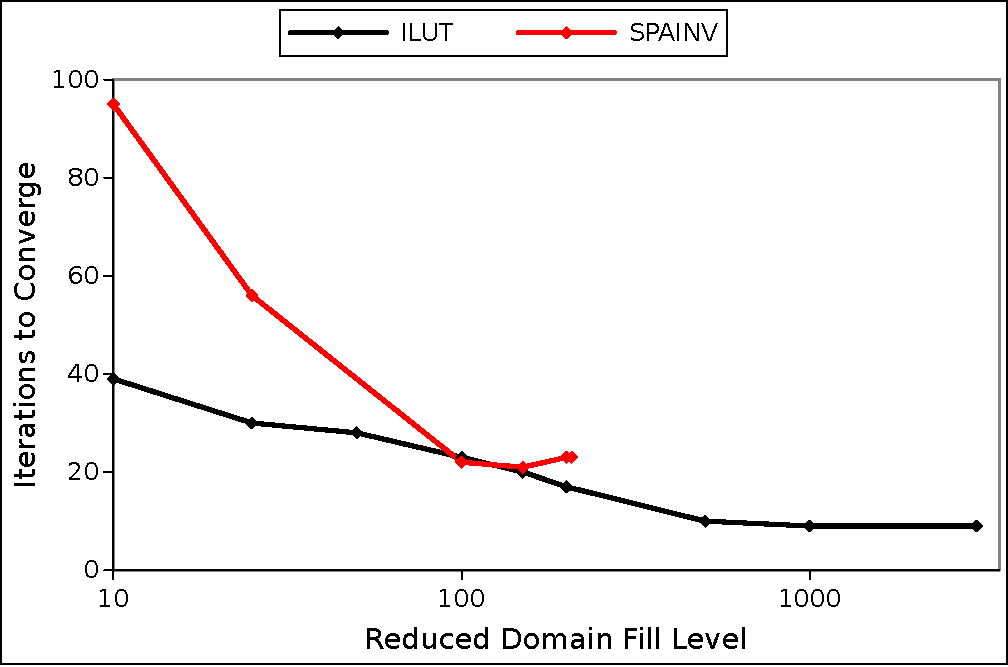
\includegraphics[width=4.25in]{chapters/spn_equations/rda_iterations.pdf}
  \end{center}
  \caption{\textbf{Number of MCSA iterations required to converge a
      single eigenvalue iteration for the fuel assembly problem with
      each preconditioning as a function of reduced domain
      approximation fill level.} \textit{The largest fill level for
      each preconditioning presented is that using the parameters that
      gave the best results without the approximation.}}
  \label{fig:rda_iterations}
\end{figure}

\begin{figure}[t!]
  \begin{center}
    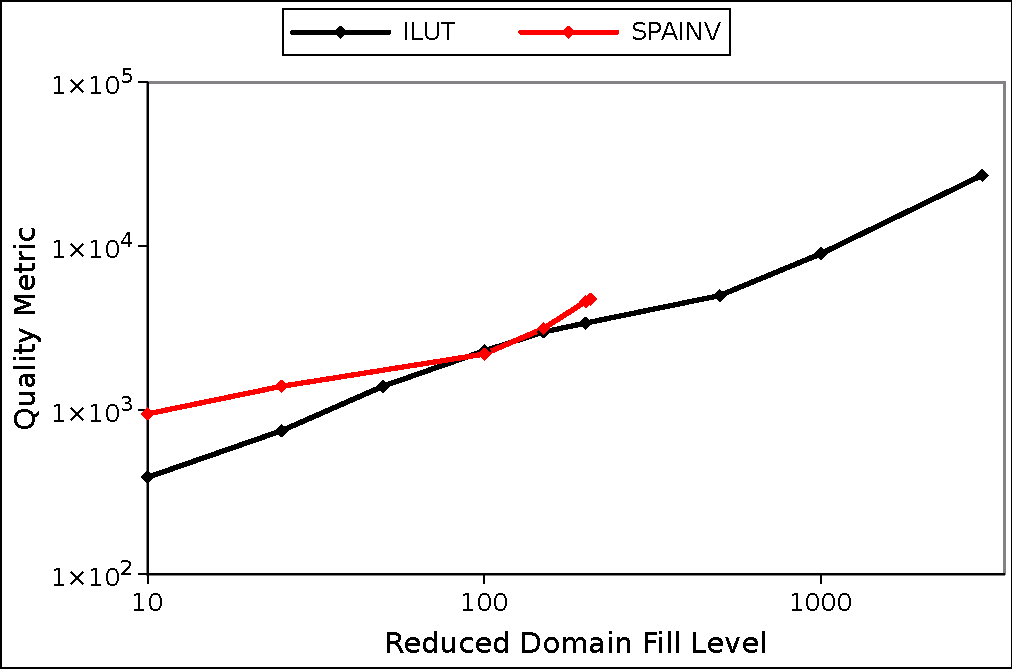
\includegraphics[width=4.25in]{chapters/spn_equations/rda_quality.pdf}
  \end{center}
  \caption{\textbf{Preconditioning quality metric for the fuel
      assembly problem given as a function of reduced domain
      approximation fill level.} \textit{The largest fill level for
      each preconditioning presented is that using the parameters that
      gave the best results without the approximation.}}
  \label{fig:rda_quality}
\end{figure}

\clearpage

%%---------------------------------------------------------------------------%%
\section{MCSA Verification\ }
\label{sec:spn_mcsa_verification}
Through the numerical studies presented in this chapter, we have
developed a set of preconditioning techniques that permit MCSA to be
used with the $SP_N$ form of the neutron transport equation and
applied to a difficult fuel assembly criticality problem. In addition,
several steps were taken to mitigate the dense composite linear
operators that arise when performing explicit MCSA preconditioning
necessary for achieve convergence. Using these results, we now compare
MCSA to conventional Krylov solvers that would be typically used to
solve the $SP_N$ form of the transport equation as presented here.

MCSA solutions to the fuel assembly problem with 1, 2, and 4 energy
groups using $SP_1$ discretization will computed using both BiCGStab
and GMRES implementations from the Trilinos scientific computing
library Aztec \cite{heroux_overview_2005}. The neutron fluxes, the
number of eigenvalue iterations required to converge the problem, and
the eigenvalue itself will be compared as a means of verification. For
the flux values, we will look at the 2-norm and infinity norm of the
relative difference vector between the reference case and the
comparison case in each energy group:
\begin{equation}
  \text{Relative Group Flux Difference} = \frac{\ve{\Phi}_{ref}^g -
    \ve{\Phi}^g}{\ve{\Phi}_{ref}^g}\:,
  \label{eq:relative_difference_vector}
\end{equation}
where the addition and subtraction operations are performed
element-wise to construct the vector. For this work, the BiCGStab
results will be taken as the reference case.

All solvers will be preconditioned with ILUT using a drop tolerance of
\sn{1}{-5} and a fill level of 5. For GMRES, no restrictions were
placed on the size of the subspace and therefore no restarts
occurred. When the collision estimator was used with MCSA, \sn{2}{4}
stochastic histories were used to compute the correction for every
energy group in the problem (\sn{4}{4} and \sn{8}{4} histories total
for the 2 and 4 group calculations respectively) corresponding to
approximately 1 stochastic history per DOF. When the expected value
estimator was used, \sn{5}{2} stochastic histories used for each
energy group (\sn{1}{3} and \sn{1.5}{3} histories total for the 2 and
4 group calculations) giving approximately 1 stochastic history for
every 5 DOFs. The reduced domain approximation was also applied in
conjunction with the ILUT preconditioning using a fill level of 100
and a threshold value of \sn{1}{-10} to reduce the density of states
in the Monte Carlo problem. For relaxation parameters, all MCSA
computations used a Neumann relaxation parameter of 0.7 while a
Richardson relaxation of 1.1 was used with the collision estimator and
1.0 with the expected value estimator. Additionally, both the
Richardson-based MCSA iteration given by Eq~(\ref{eq:mcsa}) and the
minimal residual-based MCSA iteration given by
Eq~(\ref{eq:mcsa_min_res}) will be used. A supplementary performance
analysis for this set of MCSA variations is presented in
Appendix~\ref{chap:spn_estimator_comparison}.

Table~\ref{tab:spn_solver_defs} gives definitions for the
solvers used to generate the results in the remainder of this
section. For the energy group structures,
Table~\ref{tab:spn_group_structure} gives the lower bounds of each
group in eV (an implicit upper bound of \sn{2}{6} eV is assumed for
group 0).

\begin{table}[h!]
  \begin{center}
    \begin{tabular}{ll}\hline\hline
      \multicolumn{1}{l}{\textbf{Name}} & 
      \multicolumn{1}{l}{\textbf{Definition}} \\
      BiCGStab-ILUT & BiCGStab preconditioned with ILUT \\
      GMRES-ILUT & GMRES preconditioned with ILUT \\
      MCSA-ILUT-R-C & MCSA preconditioned with ILUT using Richardson \\ 
                    & fixed point iteration and collision estimator \\
      MCSA-ILUT-MR-C & MCSA preconditioned with ILUT using minimal residual \\
                     & fixed point iteration and collision estimator \\
      MCSA-ILUT-R-EV & MCSA preconditioned with ILUT using Richardson \\
                     & fixed point iteration and expected value estimator \\
      MCSA-ILUT-MR-EV & MCSA preconditioned with ILUT using minimal residual \\
                      & fixed point iteration and expected value estimator \\
      Richardson-ILUT & Richardson iteration preconditioned with ILUT \\
      %%
      \hline\hline
    \end{tabular}
  \end{center}
  \caption{\textbf{Solver definitions used for MCSA verification and
      performance analysis.} \textit{The ILUT preconditioner
      parameters were identical for all calculations and solvers.}}
  \label{tab:spn_solver_defs}
\end{table}

\begin{table}[h!]
  \begin{center}
    \begin{tabular}{cl}\hline\hline
      \multicolumn{1}{c}{\textbf{Number of Groups}} & 
      \multicolumn{1}{l}{\textbf{Lower Bounds (eV)}} \\
      1 & \{ \sn{1}{-5} \} \\
      2 & \{ \sn{1}{-1}, \sn{1}{-5} \} \\
      4 & \{ \sn{1}{1}, \sn{1}{0}, \sn{1}{-1}, \sn{1}{-5} \} \\
      %%
      \hline\hline
    \end{tabular}
  \end{center}
  \caption{\textbf{Energy group lower bounds for the multigroup fuel
      assembly criticality problem in electron volts.} \textit{An
      implicit upper bound of \sn{2}{6} eV is assumed for group zero.}}
  \label{tab:spn_group_structure}
\end{table}

For every combination of energy group structure and solver, the
eigenvalue problem was converged with an eigensolver tolerance of
\sn{1}{-6} and a linear solver tolerance of \sn{1}{-8} in a serial
calculation. Table~\ref{tab:serial_ev_results} gives the eigenvalue
computed by each solver for each problem as well as the number of
eigenvalue iterations required to converge. For every problem, each
solver converged to the same eigenvalue up to the number of digits
reported by the eigensolver in the same number of eigenvalue
iterations.

\begin{table}[h!]
  \begin{center}
    \begin{tabular}{lccc}\hline\hline
      \multicolumn{1}{c}{\textbf{Solver}} & 
      \multicolumn{1}{c}{\textbf{Number of Groups}} & 
      \multicolumn{1}{c}{\textbf{Iterations}} &
      \multicolumn{1}{c}{\textbf{Eigenvalue}} \\
      \hline
      BiCGStab-ILUT & 1 & 25 & 1.105987 \\
      GMRES-ILUT & 1 & 25 & 1.105987 \\
      MCSA-ILUT-R-C & 1 & 25 & 1.105987 \\
      MCSA-ILUT-MR-C & 1 & 25 & 1.105987 \\
      MCSA-ILUT-R-EV & 1 & 25 & 1.105987 \\
      MCSA-ILUT-MR-EV & 1 & 25 & 1.105987 \\
      Richardson-ILUT & 1 & 25 & 1.105987 \\
      \hline
      BiCGStab-ILUT & 2 & 35 & 1.155239 \\
      GMRES-ILUT & 2 & 35 & 1.155239 \\
      MCSA-ILUT-R-C & 2 & 35 & 1.155239 \\
      MCSA-ILUT-MR-C & 2 & 35 & 1.155239 \\
      MCSA-ILUT-R-EV & 2 & 35 & 1.155239 \\
      MCSA-ILUT-MR-EV & 2 & 35 & 1.155239 \\
      Richardson-ILUT & 2 & 35 & 1.155239 \\
      \hline
      BiCGStab-ILUT & 4 & 31 & 1.175850 \\
      GMRES-ILUT & 4 & 31 & 1.175850 \\
      MCSA-ILUT-R-C & 4 & 31 & 1.175850 \\
      MCSA-ILUT-MR-C & 4 & 31 & 1.175850 \\
      MCSA-ILUT-R-EV & 4 & 31 & 1.175850 \\
      MCSA-ILUT-MR-EV & 4 & 31 & 1.175850 \\
      Richardson-ILUT & 4 & 31 & 1.175850 \\
      %%
      \hline\hline
    \end{tabular}
  \end{center}
  \caption{\textbf{Serial eigensolver verification results for the
      fuel assembly problem.} \textit{Each calculation was converged
      with the same eigensolver and linear solver
      tolerances. Table~\ref{tab:spn_solver_defs} gives the
      description for each solver type presented.}}
  \label{tab:serial_ev_results}
\end{table}

Table~\ref{tab:serial_differences_g1},
Table~\ref{tab:serial_differences_g2}, and
Table~\ref{tab:serial_differences_g4} give the infinity norms and
2-norms of the flux relative difference vectors given by
Eq~(\ref{eq:relative_difference_vector}) for all calculations and all
energy groups. In general, we see good agreement in the 2-norm between
the MCSA variants and the GMRES calculation, meaning that they have
approximately the same variation from the BiCGStab calculation. We do
note larger infinity norm values of this vector for some of the MCSA
variants relative to the GMRES results (i.e. group 1 in the 2-group
calculation), however, this large maximum value is apparently a local
phenomenon with good agreement in the 2-norm for the
calculations. Based on the good agreement between MCSA and GMRES for
the relative difference of the group fluxes and the eigenvalue results
presented here, the MCSA implementation should be deemed correct for
the fuel assembly problem for serial calculations with multiple energy
groups.

\begin{table}[h!]
  \begin{center}
    \begin{tabular}{lccc}\hline\hline
      \multicolumn{1}{c}{\textbf{Solver}} & 
      \multicolumn{1}{c}{\textbf{Group}} &
      \multicolumn{1}{c}{\textbf{$|| \cdot ||_{inf}$}} &
      \multicolumn{1}{c}{\textbf{$|| \cdot ||_2$}} \\
      \hline
      GMRES-ILUT & 0 & \sn{4.562}{-6} & \sn{6.746}{-5} \\
      MCSA-ILUT-R-C & 0 & \sn{2.099}{-5} & \sn{2.541}{-4} \\
      MCSA-ILUT-MR-C & 0 & \sn{4.812}{-5} & \sn{4.672}{-4} \\
      MCSA-ILUT-R-EV & 0 & \sn{2.371}{-5} & \sn{2.740}{-4} \\
      MCSA-ILUT-MR-EV & 0 & \sn{3.605}{-5} & \sn{2.554}{-4} \\
      Richardson-ILUT & 0 & \sn{1.531}{-5} & \sn{2.771}{-4} \\
      \hline\hline
    \end{tabular}
  \end{center}
  \caption{\textbf{Serial scalar flux verification results for the
      1-group fuel assembly problem.} \textit{The infinity norm and
      2-norm of the relative flux vector in each group is given with
      BiCGStab used as the reference. Each calculation was converged
      with the same eigensolver and linear solver
      tolerances. Table~\ref{tab:spn_solver_defs} gives the
      description for each solver type presented.}}
  \label{tab:serial_differences_g1}
\end{table}

\begin{table}[h!]
  \begin{center}
    \begin{tabular}{lccc}\hline\hline
      \multicolumn{1}{c}{\textbf{Solver}} & 
      \multicolumn{1}{c}{\textbf{Group}} &
      \multicolumn{1}{c}{\textbf{$|| \cdot ||_{inf}$}} &
      \multicolumn{1}{c}{\textbf{$|| \cdot ||_2$}} \\
      \hline
      GMRES-ILUT & 0 & \sn{7.590}{-6} & \sn{1.234}{-4} \\
      MCSA-ILUT-R-C & 0 & \sn{5.308}{-6} & \sn{1.066}{-4} \\
      MCSA-ILUT-MR-C & 0 & \sn{6.388}{-5} & \sn{2.233}{-4} \\
      MCSA-ILUT-R-EV & 0 & \sn{4.197}{-5} & \sn{2.168}{-4} \\
      MCSA-ILUT-MR-EV & 0 & \sn{2.736}{-5} & \sn{8.160}{-5} \\
      Richardson-ILUT & 0 & \sn{3.976}{-6} & \sn{7.059}{-5} \\
      \hline
      GMRES-ILUT & 1 & \sn{7.579}{-6} & \sn{1.246}{-4} \\
      MCSA-ILUT-R-C & 1 & \sn{1.645}{-5} & \sn{1.210}{-4} \\
      MCSA-ILUT-MR-C & 1 & \sn{6.635}{-4} & \sn{9.435}{-4} \\
      MCSA-ILUT-R-EV & 1 & \sn{1.797}{-4} & \sn{2.983}{-4} \\
      MCSA-ILUT-MR-EV & 1 & \sn{1.556}{-4} & \sn{2.055}{-4} \\
      Richardson-ILUT & 1 & \sn{4.031}{-6} & \sn{7.110}{-5} \\
      \hline\hline
    \end{tabular}
  \end{center}
  \caption{\textbf{Serial scalar flux verification results for the
      2-group fuel assembly problem.} \textit{The infinity norm and
      2-norm of the relative flux vector in each group is given with
      BiCGStab used as the reference. Each calculation was converged
      with the same eigensolver and linear solver
      tolerances. Table~\ref{tab:spn_solver_defs} gives the
      description for each solver type presented.}}
  \label{tab:serial_differences_g2}
\end{table}

\begin{table}[h!]
  \begin{center}
    \begin{tabular}{lccc}\hline\hline
      \multicolumn{1}{c}{\textbf{Solver}} & 
      \multicolumn{1}{c}{\textbf{Group}} &
      \multicolumn{1}{c}{\textbf{$|| \cdot ||_{inf}$}} &
      \multicolumn{1}{c}{\textbf{$|| \cdot ||_2$}} \\
      \hline
      GMRES-ILUT & 0 & \sn{2.376}{-5} & \sn{4.043}{-4} \\
      MCSA-ILUT-R-C & 0 & \sn{2.639}{-5} & \sn{3.950}{-4} \\
      MCSA-ILUT-MR-C & 0 & \sn{3.958}{-5} & \sn{4.635}{-4} \\
      MCSA-ILUT-R-EV & 0 & \sn{2.749}{-5} & \sn{3.975}{-4} \\
      MCSA-ILUT-MR-EV & 0 & \sn{2.969}{-5} & \sn{4.054}{-4} \\
      Richardson-ILUT & 0 & \sn{2.189}{-5} & \sn{3.791}{-4} \\
      \hline
      GMRES-ILUT & 1 & \sn{2.271}{-5} & \sn{3.952}{-4} \\
      MCSA-ILUT-R-C & 1 & \sn{3.701}{-5} & \sn{3.933}{-4} \\
      MCSA-ILUT-MR-C & 1 & \sn{3.803}{-5} & \sn{3.933}{-4} \\
      MCSA-ILUT-R-EV & 1 & \sn{4.142}{-5} & \sn{4.011}{-4} \\
      MCSA-ILUT-MR-EV & 1 & \sn{2.723}{-5} & \sn{4.030}{-4} \\
      Richardson-ILUT & 1 & \sn{2.137}{-5} & \sn{3.768}{-4} \\
      \hline
      GMRES-ILUT & 2 & \sn{2.310}{-5} & \sn{4.021}{-4} \\
      MCSA-ILUT-R-C & 2 & \sn{2.490}{-5} & \sn{3.956}{-4} \\
      MCSA-ILUT-MR-C & 2 & \sn{2.214}{-5} & \sn{3.608}{-4} \\
      MCSA-ILUT-R-EV & 2 & \sn{4.456}{-5} & \sn{3.833}{-4} \\
      MCSA-ILUT-MR-EV & 2 & \sn{3.366}{-5} & \sn{3.797}{-4} \\
      Richardson-ILUT & 2 & \sn{2.143}{-5} & \sn{3.767}{-4} \\
      \hline
      GMRES-ILUT & 3 & \sn{2.335}{-5} & \sn{4.029}{-4} \\
      MCSA-ILUT-R-C & 3 & \sn{3.045}{-5} & \sn{3.963}{-4} \\
      MCSA-ILUT-MR-C & 3 & \sn{2.696}{-5} & \sn{3.606}{-4} \\
      MCSA-ILUT-R-EV & 3 & \sn{1.947}{-5} & \sn{4.283}{-4} \\
      MCSA-ILUT-MR-EV & 3 & \sn{3.295}{-5} & \sn{3.837}{-4} \\
      Richardson-ILUT & 3 & \sn{2.161}{-5} & \sn{3.772}{-4} \\
      \hline\hline
    \end{tabular}
  \end{center}
  \caption{\textbf{Serial scalar flux verification results for the
      4-group fuel assembly problem.} \textit{The infinity norm and
      2-norm of the relative flux vector in each group is given with
      BiCGStab used as the reference. Each calculation was converged
      with the same eigensolver and linear solver
      tolerances. Table~\ref{tab:spn_solver_defs} gives the
      description for each solver type presented.}}
  \label{tab:serial_differences_g4}
\end{table}
 
\clearpage 

%%---------------------------------------------------------------------------%%
\section{MCSA Performance Comparison to Conventional Methods\ }
\label{sec:spn_comparison}
With the same set of solver parameters used for verification
caluclation, MCSA will now be compared to the same Krylov solvers in
terms of both iterative performance and CPU timing. A Richardson
iteration solution will also be used in order to assess the
acceleration provided by the residual Monte Carlo component of MCSA.
To compare iterative performance, the number of linear solver
iterations required to converge each eigenvalue iteration was recorded
and then averaged over all eigenvalue iterations for each
solver. 

Table~\ref{tab:spn_comparison_iterations} gives the average number of
linear solver iterations required to converge a single eigenvalue
iteration of the fuel assembly problem as a function of the number of
energy groups. In general, the iterative performance of all the
solvers tested aside from the Richardson iteration is comparable with
BiCGStab performing the best. We expect this because not only are the
multigroup $SP_N$ equations positive-definite, but they are also
block-symmetric and therefore we expect the conjugate gradient-based
methods to perform well due to the structure of the projection
scheme. It important to note that the iterative performance of each
solver is not a strong function of the number of energy groups in the
problem (and therefore the problem size). Even more important,
although BiCGStab produced the best iterative results, MCSA did
perform better than GMRES in many cases with the Richardson iteration
clearly accelerated by the Monte Carlo solve. When compared to the
preconditioned Richardson iteration, the acceleration provided by MCSA
is clear with 3-4 times fewer iterations required for convergence.

It is also important to note the reduced domain approximation
parameters, particularly the fill level, were fixed as the number of
energy groups was increased. By fixing the fill level, we are
effectively fixing the amount of information contained in the
composite linear operator available for the Monte Carlo
problem. Limiting this information to 100 entries per row in the
preconditioned system did not appear to have a significant effect on
the iterative performance of the solver. For larger numbers of energy
groups (and therefore DOFs) this may be an issue and this number may
need to be increased to maintain iterative performance. Currently,
memory restrictions arising from the explicit preconditioning strategy
prevent larger numbers of energy groups to be analyzed using an
appropriate preconditioner for the fuel assembly problem.

\begin{table}[h!]
  \begin{center}
    \begin{tabular}{lccc}\hline\hline
      \multicolumn{1}{l}{Solver}&
      \multicolumn{1}{c}{1 Group}&
      \multicolumn{1}{c}{2 Groups}&
      \multicolumn{1}{c}{4 Groups}\\
      \hline
      BiCGStab-ILUT & 11.6 & 11.6 & 12.4 \\ 
      GMRES-ILUT & 18.1 & 17.9 & 18.9 \\
      MCSA-ILUT-R-C & 14.6 & 15.4 & 17.6 \\
      MCSA-ILUT-MR-C & 16.0 & 17.1 & 23.7 \\
      MCSA-ILUT-R-EV & 18.3 & 19.4 & 16.8 \\
      MCSA-ILUT-MR-EV & 19.6 & 22.4 & 17.5 \\
      Richardson-ILUT & 60.9 & 60.4 & 63.4 \\
      %%
      \hline\hline
    \end{tabular}
  \end{center}
  \caption{\textbf{Average number of linear solver iterations
      iterations required to converge the fixed source $SP_N$ problem
      at each eigenvalue iteration for the fuel assembly problem for
      1, 2 and 4 energy groups.} \textit{Values are rounded to the
      first decimal place. Table~\ref{tab:spn_solver_defs} gives the
      description for each solver type presented.}}
  \label{tab:spn_comparison_iterations}
\end{table}

Although iterative performance for MCSA was comparable to that
observed for Krylov implementations using exactly the same
preconditioning scheme, timing performance is not as
competitive. Figure~\ref{fig:spn_comparison_time} gives the average
CPU time per linear solver iteration required to converge the fuel
assembly problem with all linear solver iterations over all eigenvalue
iterations used to compute the average. The Krylov solver
implementations are approximately an order of magnitude faster than
the MCSA implementations presented here. We expect these results for
several reasons. First, even when the reduced domain approximation is
used there are $O(100)$ elements in each row of the system and each of
those elements must be processed during a transition in the Monte
Carlo random walk sequence. In addition, although the preconditioned
fixed point iterations used in the MCSA sequence do not use the
composite linear operator but rather a sequence of matrix vector
multiplies to achieve the same preconditioning effect, they do use the
explicitly extracted inverse of the preconditioning matrices which
themselves are dense, leading to exceedingly slow computation times
even in the fixed point iteration.

For the Krylov methods, the ILUT preconditioners are applied to a
vector with two triangular solves, one for each triangular
factor. Also, the original linear operator has $O(10)$ elements in
each row of the system, an order of magnitude less than that used in
the reduced domain composite operator. Second, the implementation
presented here has not been optimized and it is likely that several
components of the algorithm can be implemented in a more desirable
time complexity. However, it is most important to note here that the
CPU timing data presented in Figure~\ref{fig:spn_comparison_time}
shows that all methods have the same time complexity; their
differences are merely the manifestation of a large time constant due
to the effects of the explicit preconditioning scheme. For transport
systems where this is not a problem, the literature explicitly shows
that MCSA can be competitive with these production Krylov methods
using CPU time as a measure \cite{evans_monte_2012}.

\begin{figure}[t!]
  \begin{center}
    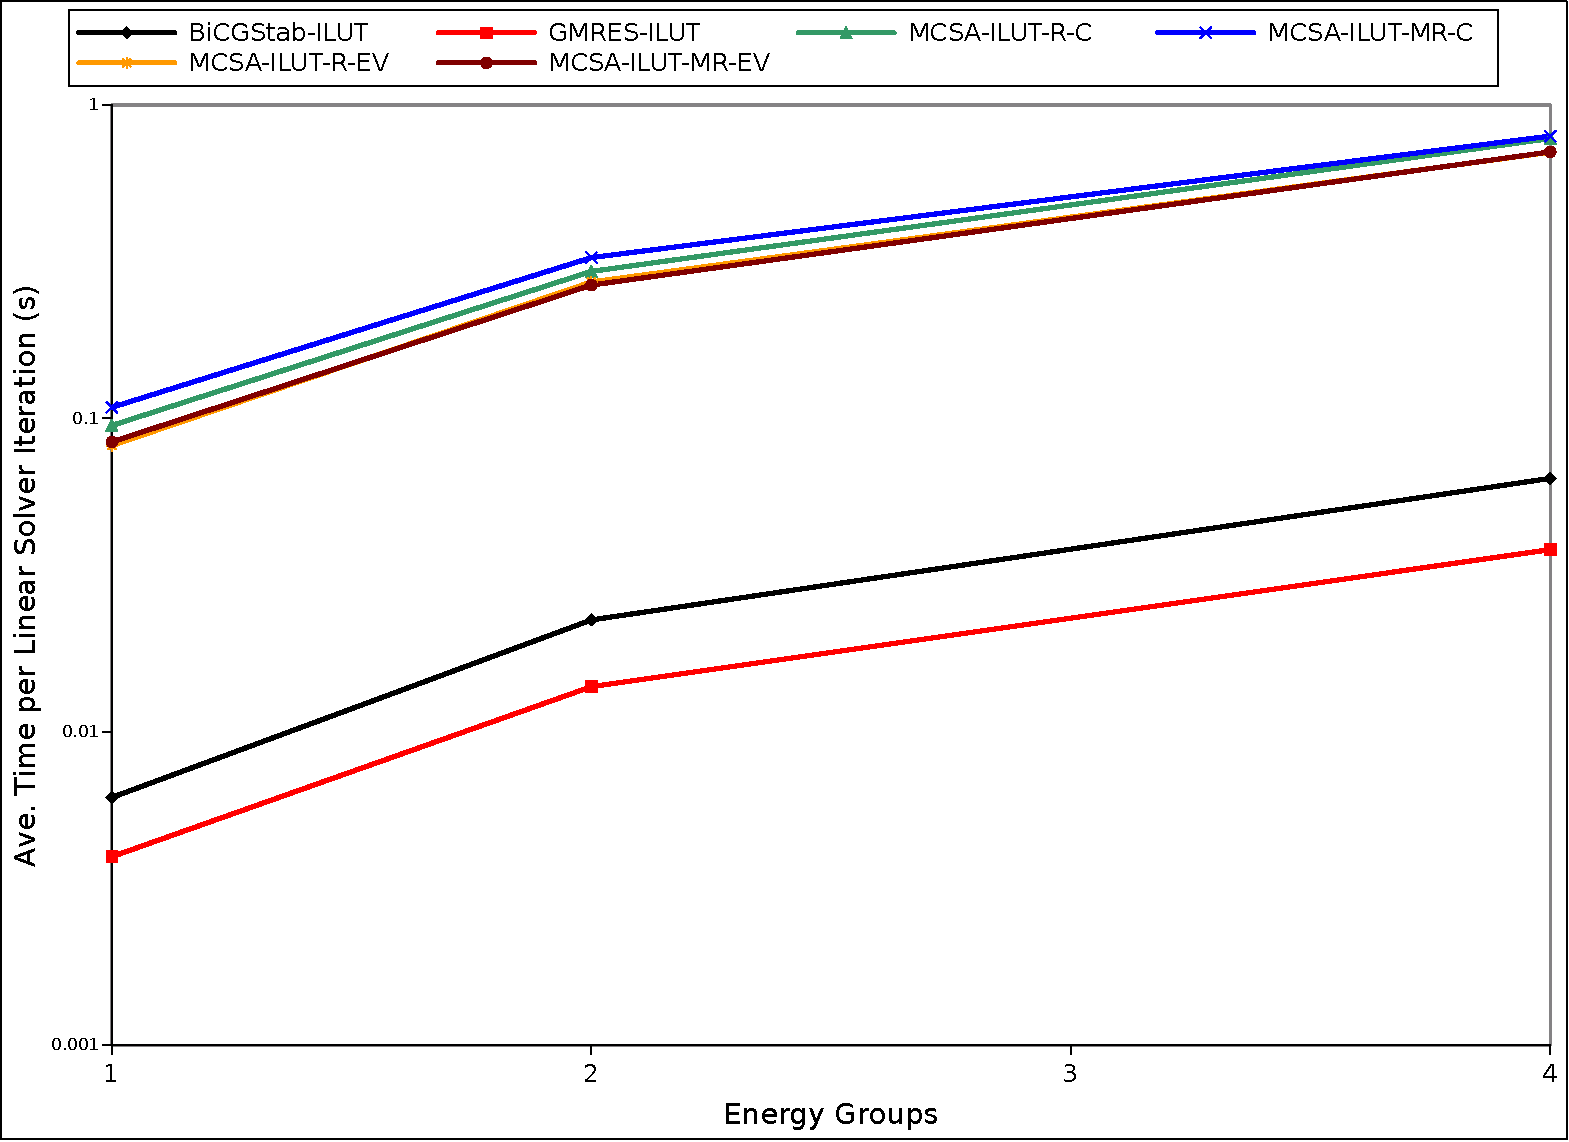
\includegraphics[width=5in]{chapters/spn_equations/solver_time.pdf}
  \end{center}
  \caption{\textbf{Average CPU time per linear solver iteration in
      seconds for the fuel assembly problem as a function of energy
      groups.}  \textit{All linear solver iterations over all
      eigenvalue iterations were used to compute the
      average. Table~\ref{tab:spn_solver_defs} gives the description
      for each solver type presented in the legend with the Krylov
      solvers represented in black and the MCSA solvers represented in
      red.}}
  \label{fig:spn_comparison_time}
\end{figure}

Finally, not considered in Figure~\ref{fig:spn_comparison_time} is the
time required to actually form the explicit inverse preconditioner
matrices and the composite operator through matrix-matrix
multiplication. The timing numbers reported were simply to perform the
MCSA iteration procedure with the composite operator already
formed. Figure~\ref{fig:spn_comparison_prec_time} additionally
presents the CPU times for MCSA convergence with the time to form the
inverse of the preconditioners and the composite linear operator
through matrix-matrix multiplication amortized over all iterations. As
is readily observed, including the costs of these operations increases
the MCSA computation time by another order of magnitude.

\begin{figure}[t!]
  \begin{center}
    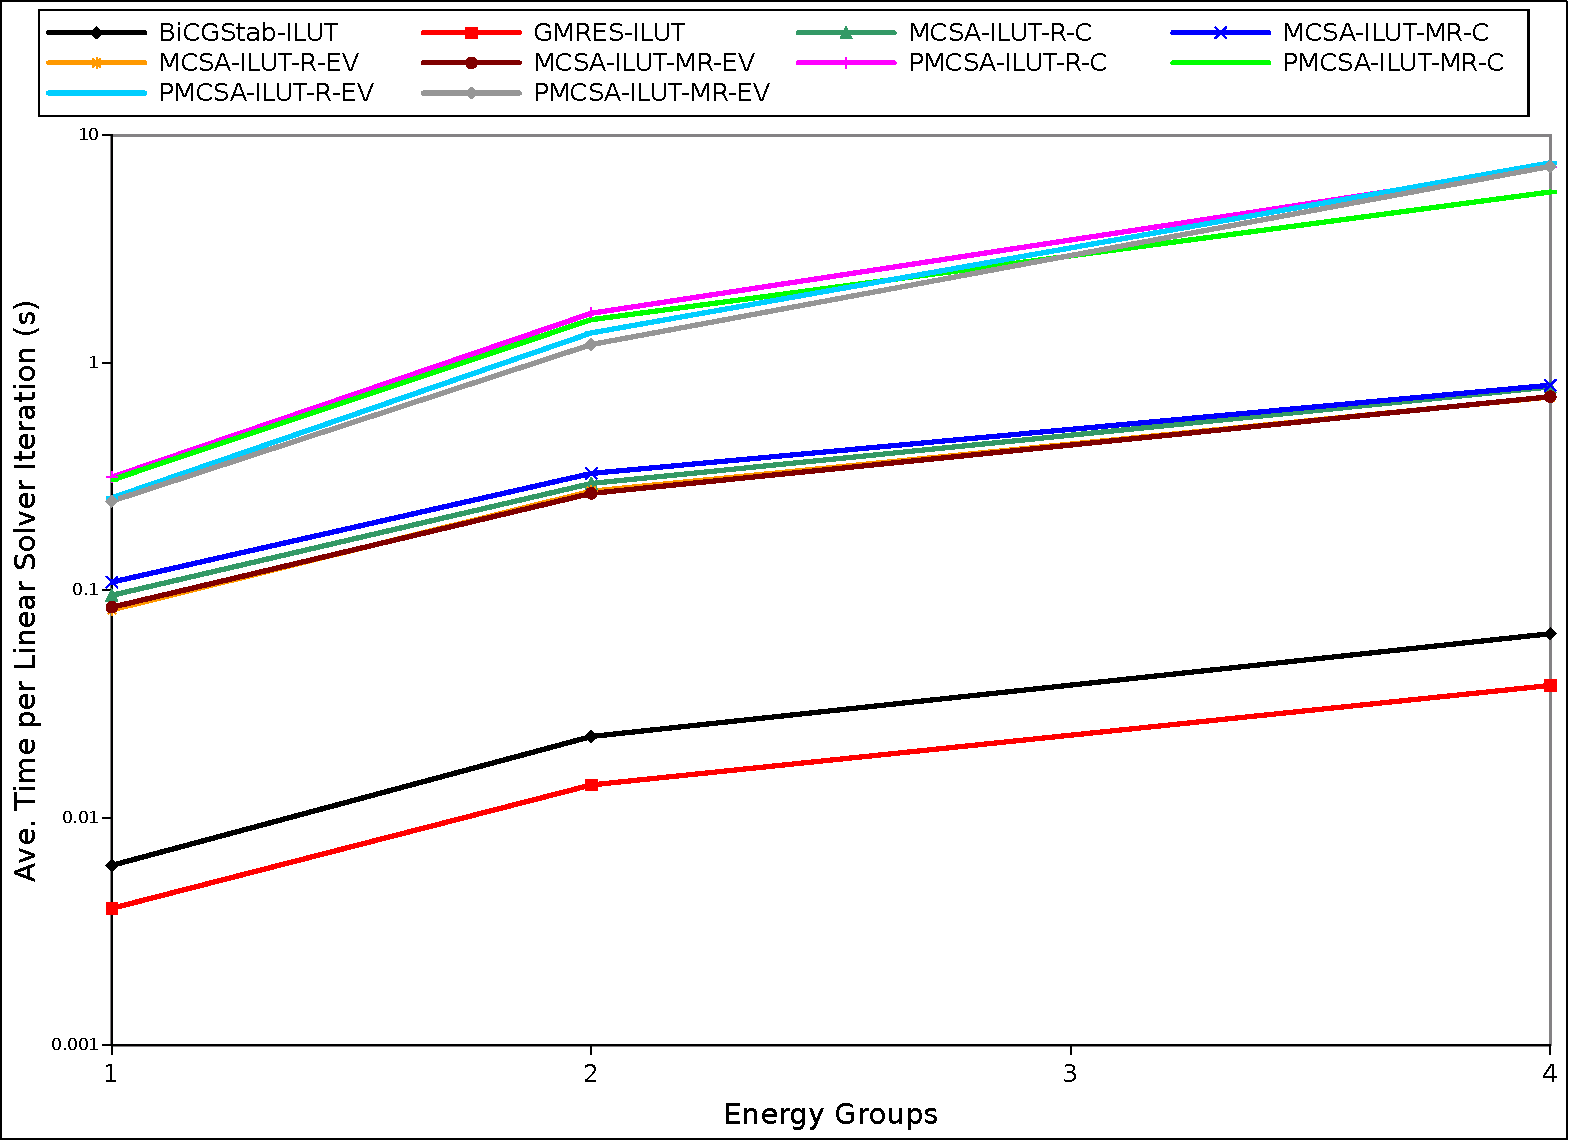
\includegraphics[width=5in]{chapters/spn_equations/solver_p_time.pdf}
  \end{center}
  \caption{\textbf{Average CPU time per iteration in seconds for the
      fuel assembly problem as a function of energy groups with
      preconditioning time included for the MCSA methods.}
    \textit{All linear solver iterations over all eigenvalue
      iterations were used to compute the
      average. Table~\ref{tab:spn_solver_defs} gives the description
      for each solver type presented in the legend. Data labeled
      starting with PMCSA and shown in blue is identical to those
      labeled with MCSA except that they additionally include the cost
      of generating the inverse of the preconditioners and composite
      linear operator.}}
  \label{fig:spn_comparison_prec_time}
\end{figure}

Based on the performance results in this section, MCSA shows promise
as a competitive and perhaps even superior method for solutions to the
neutron transport problem discretized with the $SP_N$
approximation. Not only are the correct answers produced when compared
to production linear solvers, but the iterative performance is
comparable to Krylov methods with identical preconditioning that would
typically be used every-day calculations. From a CPU timing
perspective, the methods yield the same time complexity as a function
of the number of energy groups in the problem when compared to the
Krylov methods. Here, a large time constant is generated due to the
explicit preconditioning strategy and the generation of dense linear
operators as a result. To improve these results and put general MCSA
schemes into a performance regime where they are competitive with
Krylov methods for neutron transport problems, significant research
will be required to improve upon the explicit preconditioning scheme
presented here.

\clearpage

%%---------------------------------------------------------------------------%%
\section{Summary\ }
\label{sec:mc_summary}

In this chapter, the Monte Carlo Synthetic Acceleration method has
been applied to the $SP_N$ discretization of the neutron transport
equation and explored in the context of a difficult nuclear fuel
assembly criticality problem. The following are the significant
observations and findings.

\begin{itemize}
\item MCSA can solve the asymmetric system generated by the $SP_N$
  equations
\item MCSA has been incorporated into the Exnihilo neutronics
  production code base developed at Oak Ridge National Laboratory
\item Simple Jacobi-based preconditioning reduces the spectral radius
  of the $SP_N$ system below unity, however, this alone is not
  sufficient for MCSA convergence
\item As the spectral radius approaches unity, MCSA was demonstrated
  to break down with more stochastic histories required for
  convergence and more CPU time required per history
\item Light water reactor problems are difficult to solve with MCSA as
  they have large spectral radii due to the neutron scattering in the
  moderator
\item Advanced algebraic preconditioning strategies were applied to
  the $SP_N$ equations to obtain convergence with ILUT chosen for
  subsequent investigations
\item The reduced domain approximation was required to mitigate the
  memory and performance constraints of the explicit preconditioning
  strategy although both remain significant obstacles
\item MCSA relaxation parameters were developed and observed to
  enhance the time to solution for the fuel assembly criticality
  problem
\item MCSA was verified to produce the same k-eigenvalue for the fuel
  assembly as production Krylov methods and gave good relative flux
  agreement
\item MCSA was observed to converge in fewer iterations per eigenvalue
  iteration than GMRES for the fuel assembly criticality problem and
  more than Bi-CGStab using the same preconditioning
\item The explicit preconditioning strategy required to overcome the
  MCSA spectral radius restriction creates runtimes $O(100)$ larger
  than the production Krylov methods for the fuel assembly criticality
  problem
\end{itemize}

\chapter{Monte Carlo Synthetic Acceleration Methods for the
  Navier-Stokes \\Equations\ }
\label{ch:nonlinear_problem}
Nonlinear transport problems are a common occurrence in single and
multiple physics problems in nuclear engineering. Systems of partial
differential equations, such as the Navier-Stokes equations that
describe fluid flow, yield discrete sets of stiff equations with
nonlinearities present in the variables when discretized by
conventional methods. These sets of equations characterize momentum
and energy transport through diffusion, viscous forces and convection,
and inertial forces. Traditionally, such systems have been solved by
linearizing them in a form where the nonlinearities in the variables
are eliminated and more traditional linear methods can be used for
solutions. Often characterized as segregated methods where physics
operators are split and their action on the system approximated in
steps, such methods lack consistency and accuracy in resolving the
nonlinear component of the solution. In the last 30 years, fully
consistent nonlinear methods based on Newton's method have become more
popular and many advances have been made in the nuclear engineering
field to employ these methods.

In the context of solving standalone linear systems, Monte Carlo
methods do not provide significant merit over subspace methods due to
the fact that the linear operator must be explicitly formed. For many
applications including higher fidelity neutron transport
discretizations beyond the $SP_N$ equations solved in the previous
chapter, such a requirement is prohibitive and perhaps not even
feasible to implement. Therefore, a discrete Monte Carlo solution
method is best suited for situations in which the operator is readily,
if not naturally, formed. Modern nonlinear methods meet this
requirement with Newton methods used in conjunction with Krylov
methods operating on a fully formed matrix for a robust solution
strategy. Furthermore, modern techniques exist that permit the
automatic construction of the Jacobian operator generated within a
Newton method based on the nonlinear residual evaluations, providing
all of the components necessary for a Monte Carlo solver to provide
value.

We therefore devise a new nonlinear method based on the MCSA algorithm
and Newton's method. In this chapter the fundamentals of Newton's
method will be presented along with a brief discussion of inexact
Newton methods. Newton-Krylov methods, a variant of inexact Newton
methods, will be outlined along with two common techniques for
Jacobian generation as a means of defining current
practices. Following this, the new algorithm will be presented and
implementation details will be discussed. Using the new algorithm and
a production fluid physics code, a group of challenging nonlinear
benchmark problems for the Navier-Stokes equations will be used to
verify the correctness of the method relative to solutions obtained
using conventional methods in various flow regimes. Finally, we will
compare the performance of the new method against contemporary
Newton-Krylov methods for the same benchmark problems.

%%---------------------------------------------------------------------------%%
\section{Preliminaries\ }
\label{sec:nonlinear_preliminaries}
We formulate the \textit{nonlinear problem} as follows
\citep{knoll_jacobian-free_2004}:
\begin{equation}
  \ve{F}(\ve{u}) = \ve{0}\:,
  \label{eq:nonlinear_problem}
\end{equation}
where $\ve{u} \in \mathbb{R}^n$ is the solution vector and
$\ve{F}:\mathbb{R}^N \rightarrow \mathbb{R}^N$ is the function of
nonlinear residuals. We write the nonlinear system in this form so
that when an exact solution for $\ve{u}$ is achieved, all residuals
evaluate to zero. \textit{Newton's method} is a root finding algorithm
and therefore we can use it to solve Eq~(\ref{eq:nonlinear_problem})
if we interpret the exact solution $\ve{u}$ to be the roots of
$\ve{F}(\ve{u})$. Newton's method is also an iterative scheme, and we
can generate this procedure by building the Taylor expansion of the
$k+1$ iterate of the nonlinear residuals about the previous $k$
iterate:
\begin{equation}
  \ve{F}(\ve{u}^{k+1}) = \ve{F}(\ve{u}^{k}) +
  \ve{F}'(\ve{u}^{k})(\ve{u}^{k+1}-\ve{u}^{k}) +
  \frac{\ve{F}''(\ve{u}^{k})}{2}(\ve{u}^{k+1}-\ve{u}^{k})^2 + \cdots
  \:.
  \label{eq:newton_derivation_1}
\end{equation}
If we ignore the nonlinear terms in the expansion and assert that at
the $k+1$ iterate $\ve{u}^{k+1}$ is the exact solution such that
$\ve{F}(\ve{u}^{k+1}) = \ve{0}$, then we are left with the following
equality:
\begin{equation}
  -\ve{F}(\ve{u}^{k}) =
  \ve{F}'(\ve{u}^{k})(\ve{u}^{k+1}-\ve{u}^{k})\:.
  \label{eq:newton_derivation_2}
\end{equation}
We note two things of importance in
Eq~(\ref{eq:newton_derivation_2}). The first is that
$\ve{F}'(\ve{u}^{k})$ is in fact the \textit{Jacobian},
$\ve{J}(\ve{u})$, of the set of nonlinear residuals and is defined
element-wise as:
\begin{equation}
  J_{ij} = \frac{\partial F_i(\ve{u})}{\partial u_j}\:.
  \label{eq:jacobian_def}
\end{equation}
Second, we note that $(\ve{u}^{k+1}-\ve{u}^{k})$ is simply the
solution update from the $k$ iterate to the $k+1$ iterate. We will
define this update as the \textit{Newton correction} at the $k$
iterate, $\delta \ve{u}^k$. To finish, we can then rearrange
Eq~(\ref{eq:newton_derivation_2}) to define the Newton iteration
scheme for nonlinear problems:
\begin{subequations}
  \begin{gather}
    \ve{J}(\ve{u}) \delta \ve{u}^k = -\ve{F}(\ve{u}^{k})\\
    \ve{u}^{k+1} = \ve{u}^k + \delta \ve{u}^k\:.
  \end{gather}
  \label{eq:newton_iteration}
\end{subequations}
There are then three distinct steps to perform: evaluation of the
nonlinear residuals using the solution at the $k$ iterate, the
solution of a linear system to compute the Newton correction where the
Jacobian matrix of the nonlinear equation set is the linear operator,
and the application of the correction to the previous iterate's
solution to arrive at the next iterate's solution. In the asymptotic
limit, the iterations of Newton's method will converge the nonlinear
residual quadratically \citep{kelley_iterative_1995}. Convergence
criteria is set for stopping the iteration sequence based on the
nonlinear residual. Commonly, the following criteria is used:
\begin{equation}
  ||\ve{F}(\ve{u}^{k})|| < \epsilon ||\ve{F}(\ve{u}^{0})||\:,
  \label{eq:newton_stopping_criteria}
\end{equation}
where $\epsilon$ is a user defined tolerance parameter. 

Newton's method is \textit{consistent} in that all components of the
nonlinear functions that describe the physics we are modeling are
updated simultaneously in the iteration sequence with respect to one
another. This is in comparison to \textit{inconsistent} strategies,
such as a pressure correction strategy for solving the Navier-Stokes
equations \citep{pletcher_computational_1997}, where the components of
$\ve{u}$ are updated in a staggered fashion depending on the
particular equations that they are associated with.

\subsection{Inexact Newton Methods}
\label{subsec:inexact_newton_methods}
Inexact Newton methods arise when the Jacobian operator is not exactly
inverted, resulting in an inexact Newton correction as initially
described by Dembo and others \citep{dembo_inexact_1982}. For common
sparse nonlinear systems, which in turn yield a sparse Jacobian
matrix, this situation occurs when conventional iterative methods are
applied. In their definition, Dembo formulated inexact methods such
that they are independent of the linear method used to solve for the
Newton correction and therefore are amenable to use with any linear
solver. Furthermore, they bind the convergence of the outer nonlinear
iteration to the inner linear iteration such that:
\begin{equation}
  ||\ve{J}(\ve{u}^k)\delta \ve{u}^k + \ve{F}(\ve{u}^k)|| \leq \eta^k
  ||\ve{F}(\ve{u}^k)||\:,
  \label{eq:inexact_newton_forcing}
\end{equation}
where $\eta^k \in [0,1)$ is defined as the \textit{forcing term} at
  the $k$ iterate. Eq~(\ref{eq:inexact_newton_forcing}) then states
  that the residual generated by the linear solver is bound by the
  nonlinear residual and how tightly it is bound is defined by the
  forcing term. This is useful in that we can vary how tightly coupled
  the convergence of the linear iterations used to generate the Newton
  correction is to the nonlinear iteration by relaxing or tightening
  the convergence properties on the linear iterative method. As a
  result, strategies for determining the forcing term can vary
  depending on the problem type and can greatly affect the convergence
  of the method or even prohibit convergence
  \citep{eisenstat_choosing_1996}. In addition, \textit{globalization
    methods} may be used to modify the Newton correction in a more
  desirable direction such that convergence properties can be
  improved when the initial guess for $\ve{u}$ is poor
  \citep{pawlowski_globalization_2006}.

\subsection{Newton-Krylov Methods\ }
\label{subsec:newton_krylov_methods}
A form of inexact Newton methods, \textit{Newton-Krylov methods} are
nonlinear iterative methods that leverage a Krylov subspace method as
the linear solver for generating the Newton correction
\citep{kelley_iterative_1995}. As outlined in
Appendix~\ref{ch:linear_problem}, Krylov methods are robust and enjoy
efficient parallel implementations on modern
architectures. Furthermore, their lack of explicit dependence on the
operator make them easier to implement than other
methods. Additionally, although many iterations can become memory
intensive due to the need to store the Krylov subspace for the
orthogonalization procedure, at each nonlinear iteration this cost is
reset as the Jacobian matrix will change due to its dependence on the
solution vector. This means that for every nonlinear iteration, a
completely new linear system is formed for generating the Newton
correction and we can modify the Krylov solver parameters accordingly
to accommodate this. In most nonlinear problems, the Jacobian operator
is generally non-symmetric and therefore either Krylov methods with
long recurrence relations that can handle non-symmetric systems must
be considered or the Newton correction system must be preconditioned
such that the operator is symmetric and short recurrence relation
methods can be potentially be used.

With many Krylov methods available, which to use with the Newton
method is dependent on many factors including convergence rates and
memory usage. Several studies have been performed to investigate this
\citep{mchugh_inexact_1993,knoll_newton-krylov_1995}. In their
numerical studies in 1995, Knoll and McHugh used the set of highly
nonlinear and stiff convection-diffusion-reaction equations to solve a
set of tokamak plasma problems with the goal of measuring solver
performance with Newton's method. They note several trade-offs in
using Krylov methods with the Newton solver. The first is that the
optimization condition that results from the constraints (e.g. the
minimization of the GMRES residual over the Krylov space) can be
relaxed by restricting the size of the subspace such that only a fixed
number of subspace vectors may be maintained, thus reducing memory
requirements. 

We can also relax the optimization condition by instead restarting the
recurrence relation with a new set of vectors once a certain number of
vectors have been generated. The optimization condition is maintained
over that particular set of vectors, however, Knoll and McHugh note
that this ultimately slows the convergence rate as compared to keeping
all vectors as the new set of vectors is not necessarily orthogonal to
the previous set, and therefore not optimal over the entire iteration
procedure. The orthogonality condition can be relaxed by using a
recurrence relation that does not generate a strictly orthonormal
basis for the Krylov subspace such as the Lanzcos biorthogonalization
procedure, resulting in memory savings due to the shorter Lanzcos
recurrence relation. Based on their numerical analysis, they observed
GMRES to be the most robust for any given nonlinear problem and
therefore used it for subsequent work in this area.

\subsection{Jacobian-Free Approximation}
\label{subsec:jacobian_free_approximation}
In many cases, the Jacobian is difficult to form from the difference
equations and costly to evaluate for large equation sets. For simple
nonlinear cases such as the Navier-Stokes equations, the derivatives
can be computed and coded, but due to the complexity of those
derivatives and the resulting difference equations this task can be
tedious, error prone, and must be repeated for every equation
set. Furthermore, in their 1995 work, Knoll and McHugh also noted that
a dominating part of their computation time was the evaluation of the
difference equations for building the Jacobian
\citep{knoll_newton-krylov_1995}. By recognizing that Krylov methods
only need the action of the operator on a vector instead of the
operator itself, the Jacobian can instead be approximated through
various numerical methods including a difference-based Jacobian-free
formulation.

Jacobian-Free methods, and in particular \textit{Jacobian-Free
  Newton-Krylov} (JFNK) methods \citep{knoll_jacobian-free_2004}, rely
on forming the action of the Jacobian on a vector as required by the
Krylov solver through a forward difference scheme. In this case, the
action of the Jacobian on some vector $\ve{v}$ is given as:
\begin{equation}
  \ve{J}(\ve{u})\ve{v} = \frac{\ve{F}(\ve{u} + \epsilon \ve{v}) -
    \ve{F}(\ve{u})}{\epsilon}\:,
  \label{eq:jacobian_free_product}
\end{equation}
where $\epsilon$ is a small number typically on the order of machine
precision. Kelley \citep{kelley_iterative_1995} points out a potential
downfall of this formulation in that if the discretization error in
$\ve{F}(\ve{u})$ is on the order of the perturbation parameter
$\epsilon$, then the finite difference error from
Eq~(\ref{eq:jacobian_free_product}) pollutes the solution. 

In addition, Knoll and McHugh noted that for preconditioning purposes,
part of the Jacobian must still explicitly be formed periodically and
that linear solver robustness issues were magnified by the matrix-free
approach due to the first-order approximation. This formation
frequency coupled with the numerous evaluations of the Jacobian
approximation create a situation where after so many nonlinear
iterations, it becomes cheaper to instead fully form the Jacobian. For
simple equation sets, this may only take 5-10 Newton iterations to
reach this point while over 30 may be required for larger equations
sets and therefore larger Jacobians.

\subsection{Automatic Differentiation for Jacobian Generation}
\label{subsec:automatic_differentiation}
If it is acceptable to store the actual Jacobian matrix, other methods
are available to construct it without requiring hand-coding and
evaluating derivatives, thus eliminating the associated issues. In
addition, if any additional equations are added to the system or a
higher order functional approximation is desired, it would be useful
to avoid regenerating and coding these derivatives. Becoming more
prominent in the 1990's, \textit{automatic differentiation} is a
mechanism by which the derivatives of a function can be generated
automatically by evaluating it. Automatic differentiation is built on
the concept that all functions discretely represented in a computer
are ultimately represented by elementary mathematical operations. If
the chain rule is applied to those elementary operations, then the
derivatives of those functions can be computed to the order of
accuracy of their original discretization in a completely automated
way \citep{averick_computing_1994}.

The work of Bartlett and others \citep{bartlett_automatic_2006}
extended initial Fortran-based work in the area of automatic
differentiation implementations to leverage the parametric type and
operator overloading features of C++ \citep{stroustrup_c++_1997}. They
formulate the differentiation problem from an element viewpoint by
assuming that a global Jacobian can be assembled from local element
function evaluations of $e_k : \mathbb{R}^{n_k} \rightarrow
\mathbb{R}^{m_k}$, similar to the finite element assembly procedure
as:
\begin{equation}
  \ve{J}(\ve{u}) = \sum_{i=1}^N \ve{Q}^T_i \ve{J}_k \ve{P}_i\:,
  \label{eq:fad_global_jacobian}
\end{equation}
where $\ve{J}_{k_i} = \partial e_{k_i} / \partial P_i u$ is the
$k^{th}$ element function Jacobian, $\ve{Q} \in \mathbb{R}^{n_{k_i}
  \times N}$ is a projector onto the element domain and $\ve{P} \in
\mathbb{R}^{m_{k_i} \times N}$ a projector onto the element range for
$\ve{F}(\ve{u}) \in \mathbb{R}^{N \times N}$. The Jacobian matrix for
each element will therefore have entirely local data in a dense
structure, eliminating the need for parallel communication and sparse
techniques during differentiation. Only when all local differentials
are computed does communication of the Jacobian occur through
gather/scatter operations in order to properly assemble it. 

Also of benefit is the fact that element-level computations generally
consist of a smaller number of degrees of freedom, thus reducing
memory requirements during evaluation as compared to a global
formulation of the problem. Such a formulation is not limited to
finite element formulations and is amenable to any scheme where the
system is globally sparse with degrees of freedom coupled to local
domains including finite volume representations. The templating
capabilities of C++ were leveraged with the element-based evaluation
and assembly scheme as in Eq~(\ref{eq:fad_global_jacobian}) by
templating element function evaluation code on the evaluation type. If
these functions are instantiated with standard floating point types
then the residual is returned. If they are instead instantiated with
the operator-overloaded automatic differentiation types, both the
residual and Jacobian are returned.

Of interest to Bartlett, Averick, and the many others that have
researched automatic differentiation are measures of its performance
relative to hand-coded derivatives and capturing the Jacobian matrix
from matrix-free approximations. Given their element-based function
evaluation scheme, Bartlett's work varied the number of degrees of
freedom per element and compared both the floating point operation
count and CPU time for both the templated automatic differentiation
method and hand-coded derivatives for Jacobian evaluations. Although
they observed a 50\% increase in floating point operations in the
templated method over the hand-coded method, run times were observed
to be over 3 times faster for the templated method due to the fact
that the element-based formulation of the templated method is causing
better utilization of cache and therefore faster data
access. Furthermore, they observed linear scaling behavior for
automatic differentiation as the number of degrees of freedom per
element were increased. Based on these results, this type of automatic
differentiation formulation was deemed acceptable for use in
large-scale, production physics codes.

%%---------------------------------------------------------------------------%%
\section{The FANM Method\ }
\label{sec:fanm}
In production physics codes based on nonlinear equations sets,
Newton-Krylov methods are the primary means of generating a fully
consistent solution scheme
\citep{evans_development_2006,evans_enhanced_2007,gaston_parallel_2009,godoy_parallel_2012}. It
is common that for large scale simulations these problems are memory
limited due to the subspaces generated by robust Krylov methods which
may often build hundreds of vectors during a Newton step. Often, a
matrix-free approach is chosen to relax memory requirements over
directly generating the Jacobian matrix and facilitate the
implementation. However, as we observed in previous sections, these
matrix-free methods suffer from poorly scaled problems and the first
order error introduced by the Jacobian approximation. In addition, it
was observed that the savings induced by the matrix-free approach is
eventually amortized over a number of nonlinear iterations where it
becomes more efficient computationally to instead form the Jacobian.

In Chapter~\ref{ch:stochastic_methods}, we focused our efforts on
developing and improving Monte Carlo methods for inverting linear
systems. These methods, when used to accelerate a stationary method in
MCSA, enjoy exponential convergence rates. Although this requires more
storage to represent the linear system than that of a Krylov method
where the operator is not required, we do not incur any additional
storage costs once the iteration sequence begins. In the context of
nonlinear problems, the Jacobian matrix that we are required to
generate for the Monte Carlo solvers may be generated at will from the
nonlinear functions in the Newton system using automatic
differentiation. Not only do we then have a simple and automated way
to generate the Jacobian, but we also enjoy a Jacobian of numerical
precision equivalent to that of our function evaluations.

We therefore propose the \textit{Forward-Automated Newton-MCSA} (FANM)
method that utilizes all of the above components. Presented in
Algorithm~\ref{alg:fanm}, the FANM method is an inexact Newton method
where MCSA is used to compute the Newton correction. In line 3,
automatic differentiation is used at each iteration to build the
Jacobian operator which can in turn be used to build weights and
probabilities for the Monte Carlo game. In line 4, MCSA is used to
solve the linear problem for the Newton correction. As with other
inexact methods, any given forcing term can be used to control the
convergence of the MCSA iteration at every Newton step. Finally, in
line 5 the Newton correction is applied and the iteration proceeds
until convergence. In addition to forcing term adjustments, other
techniques for improving performance of the nonlinear iteration may be
used with FANM including backtracking methods.

\begin{algorithm}[h!]
  \caption{FANM Algorithm}
  \label{alg:fanm}
  \begin{algorithmic}[1]
    \State $k := 0$ 
    \While{$||\ve{F}(\ve{u}^{k})|| > \epsilon
      ||\ve{F}(\ve{u}^{0})||$} 
    \State $\ve{J}(\ve{u}^{k}) \leftarrow AD(\ve{F}(\ve{u}^k))$ 
    \Comment{Automatic differentiation} 
    \State $\ve{J}(\ve{u}^k) \delta \ve{u}^k = -\ve{F}(\ve{u}^{k})$
    \Comment{Solve for the Newton correction with MCSA} 
    \State $\ve{u}^{k+1} \leftarrow \ve{u}^k + \delta \ve{u}^k$ 
    \State $k \leftarrow k+1$ 
    \EndWhile
  \end{algorithmic}
\end{algorithm}

At first glance, FANM is simply a variant of an inexact Newton method
with a specific requirement of a fully formed Jacobian. However, FANM
has the potential to provide value in several areas. First, if
iterative or parallel performance of MCSA can be demonstrated to
better than that of GMRES or similar subspace methods for asymmetric
systems, FANM may outperform a Newton-Krylov method. Second, for
situations where memory is a constraint, especially in situations
where the Jacobian is generated often if not at every Newton
iteration, not building a subspace for ill-conditioned problems will
alleviate the associated cost. However, until the preconditioning
issues associated with MCSA as presented in the previous chapter using
the $SP_N$ equations can be resolved, this hypothesis can
unfortunately not be researched. Explicit algebraic preconditioning
used in conventional solution methods will almost certainly be
required to reduce the spectral radius of most Jacobian operators for
MCSA to apply and therefore the current preconditioning strategy will
destroy all potential memory benefits of FANM.

\clearpage

%%---------------------------------------------------------------------------%%
\section{Navier-Stokes Benchmark Problems\ }
\label{sec:ns_benchmarks}
To verify the FANM method for nonlinear problems, we choose benchmark
solutions for the 2-dimensional, steady, incompressible Navier-Stokes
equations on a rectilinear grid in much the same way as Shadid and
Pawlowski's work on Newton-Krylov methods for the solution of these
equations \citep{shadid_inexact_1997,pawlowski_globalization_2006}. We
define these equations as follows:
\begin{subequations}
  \begin{gather}
    \rho \ve{u} \cdot \nabla \ve{u} - \nabla \cdot \ve{T} - \rho
    \ve{g} = \ve{0}
    \label{eq:ns_momentum}\\
    \nabla \cdot \ve{u} = 0
    \label{eq:ns_continuity}\\
    \rho C_p \ve{u} \cdot \nabla T + \nabla \cdot \ve{q} = 0\:,
    \label{eq:ns_energy}
  \end{gather}
  \label{eq:navier_stokes}
\end{subequations}
where $\rho$ is the fluid density, $\ve{u}$ is the fluid velocity,
$C_p$ the specific heat capacity at constant pressure of the fluid,
$T$ the temperature of the fluid, and $\ve{g}$ the acceleration due to
gravity. Eq~(\ref{eq:ns_momentum}) provides momentum transport,
Eq~(\ref{eq:ns_continuity}) provides the mass balance, and
Eq~(\ref{eq:ns_energy}) provides energy transport with viscous
dissipation effects neglected. In addition, we close the system with
the following equations:
\begin{subequations}
  \begin{gather}
    \ve{T} = -P \ve{I} + \mu[\nabla \ve{u} + \nabla \ve{u}^T]
    \label{eq:ns_stress_tensor}\\
    \ve{q} = - k \nabla T\:,
    \label{eq:ns_heat_flux}
  \end{gather}
  \label{eq:ns_closure}
\end{subequations}
where $\ve{T}$ is the stress tensor, $P$ is the hydrodynamic pressure,
$\mu$ is the dynamic viscosity of the fluid, $\ve{q}$ is the heat flux
in the fluid, and $k$ is the thermal conductivity of the fluid. This
set of strongly coupled equations possesses both the nonlinearities
and asymmetries that we are seeking for qualification of the FANM
method. Further, physical parameters within these equations can be
tuned to enhance the nonlinearities. We will then apply these
equations to the following two standard benchmark problems.

\subsection{Thermal Convection Cavity Problem}
\label{subsec:natural_convection_cavity}
In 1983 a set of benchmark solutions for the natural convection of air
in a square cavity was published \citep{de_vahl_davis_natural_1983} as
shown in Figure~\ref{fig:natural_convection_cavity} for the solution
of the energy, mass, and momentum equations.

\begin{figure}[t!]
  \begin{center}
    \scalebox{1.5}{
      \input{chapters/nonlinear_problem/natural_convection_cavity.pdftex_t} }
  \end{center}
  \caption{\textbf{Problem setup for the natural convection cavity
      benchmark.} \textit{Dirichlet conditions are set for the
      temperature on the left and right while Neumann conditions are
      set on the top and bottom of the Cartesian grid. The temperature
      gradients will cause buoyancy-driven flow. Zero velocity
      Dirichlet conditions are set on each boundary. No thermal source
      was present.}}
  \label{fig:natural_convection_cavity}
\end{figure}

In this problem, a rectilinear grid is applied to the unit square. No
heat flow is allowed out of the top and bottom of the square with a
zero Neumann condition specified. Buoyancy driven flow is generated by
the temperature gradient from the hot and cold Dirichlet conditions on
the left and right boundaries of the box. By adjusting the Rayleigh
number of the fluid (and therefore adjusting the ratio of convective
to conductive heat transfer), we can adjust the influence of the
nonlinear convection term in Eq~(\ref{eq:ns_momentum}). In Shadid's
work, Rayleigh numbers of up to \sn{1}{6} were used for this benchmark.

Isotherms of the temperature solution for these equations are given in
Figure~\ref{fig:convection_isotherms} for Rayleigh numbers of
\sn{1}{3}, \sn{1}{4}, \sn{1}{5} and \sn{1}{6}. Note that as the
Rayleigh number is increased, the fluid begins to rotate in the
clockwise direction. This causes the temperature gradients to rotate
as well with the fluid, given the increased rotation observed for the
isotherms in the figure. As the Rayleigh number increases, thermal
energy and momentum transport in the system become more dominated by
convection rather than diffusion, causing the nonlinearities in the
advective derivatives to grow.

\begin{figure}[t!]
  \begin{center}
    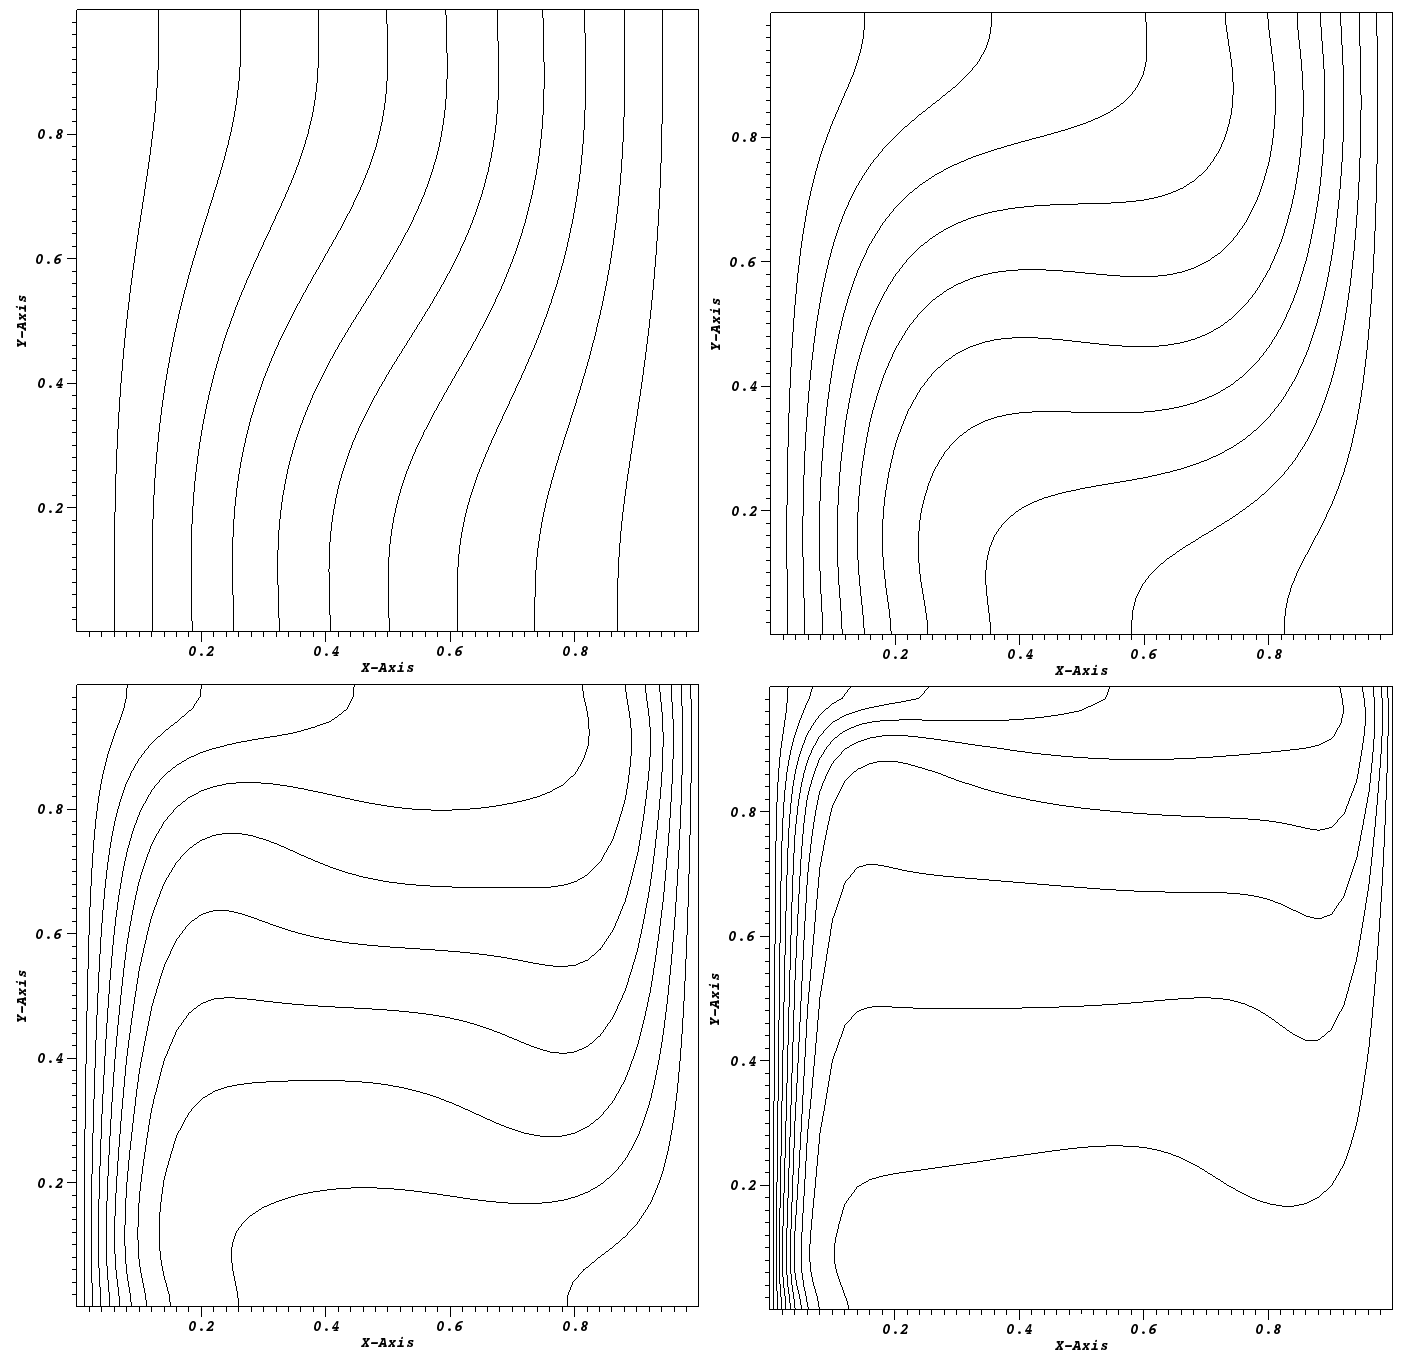
\includegraphics[width=6in]{chapters/nonlinear_problem/convection_isotherms.png}
  \end{center}
  \caption{\textbf{Isotherms from solution to the thermal convection
        cavity problem.} \textit{Top left: Ra = \sn{1}{3}; Top right:
        Ra = \sn{1}{4}; Bottom left: Ra = \sn{1}{5}; Bottom left: Ra =
        \sn{1}{6}. Isotherms on unit temperature scale from 0 to 1
        with divisions of 0.1 for each calculation.}}
  \label{fig:convection_isotherms}
\end{figure}

\clearpage

\subsection{Lid Driven Cavity Problem}
\label{subsec:lid_driven_cavity}
As an extension of the convection problem, the second benchmark
problem given by Ghia \citep{ghia_high-re_1982} adds a driver for the
flow to introduce higher Reynolds numbers into the system, providing
more inertial force to overcome the viscous forces in the fluid. The
setup for this problem is equally simple, containing only the
Dirichlet conditions as given in Figure~\ref{fig:lid_driven_cavity}
and is only applied to the mass and momentum equations on the unit
square.

\begin{figure}[t!]
  \begin{center}
    \scalebox{1.5}{
      \input{chapters/nonlinear_problem/lid_driven_cavity.pdftex_t} }
  \end{center}
  \caption{\textbf{Problem setup for the lid driven cavity benchmark.}
    \textit{Dirichlet conditions of zero are set for the velocity on
      the left and right and bottom while the Dirichlet condition set
      on the top provides a driving force on the fluid.}}
  \label{fig:lid_driven_cavity}
\end{figure}

The top boundary condition will provide a driver for the flow and its
variation will in turn vary the Reynolds number of the fluid. An
increased velocity will generate more inertial forces in the fluid,
which will overcome the viscous forces and again increase the
influence of the nonlinear terms in Eq~(\ref{eq:ns_momentum}). Shadid
used Reynolds numbers up to \sn{1}{4} for this benchmark problem.

Isocurves of the velocity magnitudes are given in
Figure~\ref{fig:driven_velocity_isocurves} for solutions to the lid
driven cavity problem at Reynolds numbers of 100, 300, 500 and
700. Increasing the velocity on the top boundary of the problem drives
up the Reynolds number of the system making it more difficult to
solve. More rotation of the fluid is induced by inertial forces and
we begin to see some additional vortices form besides the primary
vortex in the center of the box.

\begin{figure}[t!]
  \begin{center}
    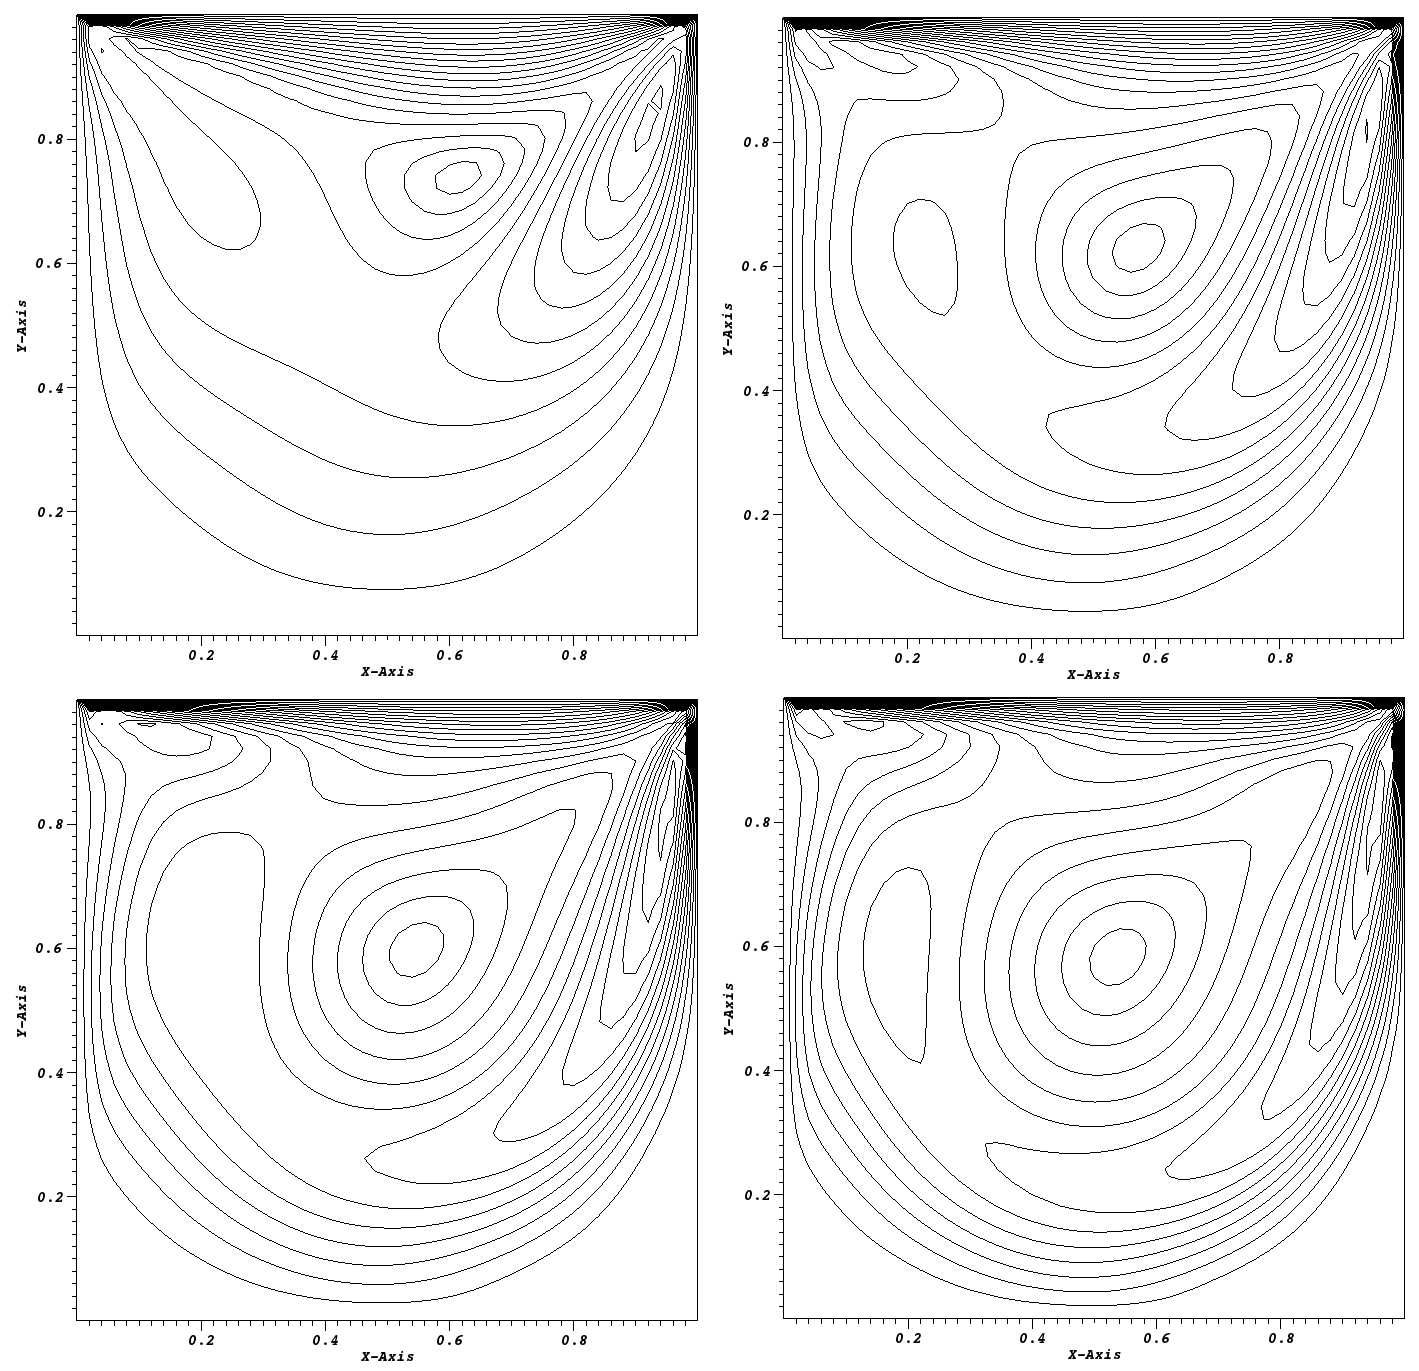
\includegraphics[width=6in]{chapters/nonlinear_problem/driven_velocity_isocurves.png}
  \end{center}
  \caption{\textbf{Velocity magnitude isocurves from solution to the
      thermal convection cavity problem.} \textit{Top left: Re = 100;
      Top right: Re= 300; Bottom left: Re = 500; Bottom left: Re =
      700. Isocurves on unit velocity scale from 0 to 1 with divisions
      of 0.05 for each calculation.}}
  \label{fig:driven_velocity_isocurves}
\end{figure}

\clearpage

%%---------------------------------------------------------------------------%%
\section{FANM Verification\ }
\label{sec:fanm_verification}

For each of the benchmark problems, we will present the results of
computations using FANM and directly compare them to results using a
Newton-Krylov method in order to verify the correctness of FANM and
its applicability to fluid problems. For each case, we will compare
the global minimum, maximum, and average values for fluid velocity,
pressure, and temperature where applicable. If the values for these
quantities computed using FANM match those computed using a production
Newton-Krylov method, the implementation will be deemed correct for
the purposes of this work. In addition, we will report the tolerance
to which the nonlinear residual was converged as an additional means
of comparison for correctness.

Given the difficulty of these benchmark problems, the linear solve at
each Newton step was preconditioned with an algebraic multigrid
method, a common technique for preconditioning these equations
\citep{ghia_high-re_1982,evans_enhanced_2007}. Without multigrid
preconditioning, the residual in MCSA was observed to
stagnate. Typically this happens because the Richardson iteration will
damp the higher order error modes on the scale of the computational
grid used to solve the problem but will miss lower order error
modes. In terms of Monte Carlo, this stagnation manifests itself in
histories that simply do no terminate and therefore no solution is
acquired.

For FANM, this preconditioning was required to reduce the spectral
radius of the Jacobian operators generated at each Newton step and for
the Newton-Krylov solutions this preconditioning was required to
obtain good convergence properties although it was not necessary for
convergence. For every benchmark calculation, both FANM and
Newton-Krylov were preconditioned with the same multigrid parameters
such that the conditioning of the system would not be a factor in the
verification of the method or the performance comparison in the
following section. As with the radiation transport calculations in the
previous chapter, algrebraic preconditioning with the multigrid method
results in dense linear systems. To mitigate this, the reduced domain
approximation was again applied to the Monte Carlo solution within the
MCSA solve occuring at each nonlinear iteration. The values used for
the approximation will be given for each benchmark problem.

Results in this and the following section were produced by the Drekar
multiphysics code base being developed at Sandia National Laboratories
for fluid flow and other multiple physics simulations
\citep{pawlowski_drekar_2012}. Drekar is a massively parallel physics
framework that utilizes Newton-Krylov methods to generate a fully
consistent solution scheme for the Navier-Stokes equations among other
systems with Jacobian generation through automatic differentiation. To
achieve these results, a Monte Carlo solver generated for this work
was injected into the nonlinear toolchain within Drekar to form an
implementation of the FANM method. For the Newton-Krylov solutions,
the same production implementation of GMRES from the Trilinos
scientific computing library Aztec \citep{heroux_overview_2005} used
for the verification of MCSA for the $SP_N$ solutions in the previous
chapter was also used here as a means of comparison and FANM
benchmarking.

\subsection{Thermal Convection Cavity Results}
\label{subsec:thermal_convection_verification}

A Drekar model of thermal convection cavity problem was solved using
both the Newton-Krylov solver and a FANM solver for Rayleigh numbers
of \sn{1}{3}, \sn{1}{4}, \sn{1}{5} and \sn{1}{6} on a $50 \times 50$
square grid. Table~\ref{tab:thermal_convection_parameters} gives the
physical parameters of the problem and
Table~\ref{tab:convection_mcsa_parameters} gives the MCSA solver
parameters used within the FANM method. Variation in the Rayleigh
number of the system was achieved by keeping the parameters given in
Table~\ref{tab:thermal_convection_parameters} constant and varying
temperature of the hot side of the cavity. In addition to multigrid
preconditioning for the linear solution at each Newton step,
backtracking as outlined in Shadid's work \citep{shadid_inexact_1997}
was used as a means of globalization to assist the Newton correction
computation while the forcing term was computed at each Newton step
using method 2 from Shadid's work. In this forcing term method,
nonlinear residuals from the two previous Newton steps are used to
inform the choice of the forcing term for the next step.

\begin{table}[h!]
  \begin{center}
    \begin{tabular}{lcc}\hline\hline
      \multicolumn{1}{l}{Parameter}& 
      \multicolumn{1}{c}{Value}&
      \multicolumn{1}{c}{Units}\\\hline
      $x_{min}$ & 0.0 & $m$ \\
      $x_{max}$ & 1.0 & $m$ \\
      $y_{min}$ & 0.0 & $m$ \\
      $y_{max}$ & 1.0 & $m$ \\
      $N_x$ & 50 & - \\
      $N_y$ & 50 & - \\
      $DOFs$ & 10404 & - \\
      Initial Temperature & 0.0 & $K$ \\
      Density & 1.0 & $kg / m^3$ \\
      Specific Heat & 1.0 & J / $(kg \times K)$ \\
      Dynamic Viscosity & 0.71 & $N \times s / m^2$ \\
      Thermal Conductivity & 1.0 & $W / (m \times K)$ \\
      Thermal Expansion Coefficient & 1000 & $1 / K$ \\
      Thermal Diffusivity & 1.0 & $m^2 / s$ \\
      Kinematic Viscosity & 0.71 & $m^2 / s$ \\
      Gravitational Acceleration & 10 & $m / s^2$ \\
      Cavity Characteristic Length & 1.0 & $m$ \\
      Prandtl Number & 0.71 & - \\
      %%
      \hline\hline
    \end{tabular}
  \end{center}
  \caption{\textbf{Thermal convection cavity FANM verification model
      problem parameters.}  \textit{The Navier-Stokes equations in 2
      dimensions are used for the model problem. The Rayleigh number
      is varied by modifying the hot boundary temperature to induce
      larger temperature gradients and bouyancy-driven flow.}}
  \label{tab:thermal_convection_parameters}
\end{table}

\begin{table}[h!]
  \begin{center}
    \begin{tabular}{lc}\hline\hline
      \multicolumn{1}{l}{Parameter}& 
      \multicolumn{1}{c}{Value}\\\hline
      Histories & 500,000 per iteration \\
      Weight Cutoff & \sn{1}{-2} \\
      Fixed Point Iteration & Richardson \\
      Estimator & Adjoint Collision \\
      Reduced Domain Fill Level & 200 \\
      %%
      \hline\hline
    \end{tabular}
  \end{center}
  \caption{\textbf{Thermal convection cavity FANM verification MCSA
      solver parameters.} \textit{No relaxation parameters or variance
      reduction techniques were used with MCSA other than the reduced
      domain approximation.}}
  \label{tab:convection_mcsa_parameters}
\end{table}

For the verification calculations, at each Rayleigh number variation
the global minimum, maximum, and average values were recorded for
fluid velocity in the x and y directions, fluid pressure, and fluid
temperature. Tables~\ref{tab:convection_ra1e3_results},
\ref{tab:convection_ra1e4_results},
\ref{tab:convection_ra1e5_results}, and
\ref{tab:convection_ra1e6_results} give the results of these
computations. It should be noted that the negative pressures computed
are due to a relative pressure being reported. For each of the data
points presented, both Newton-Krylov solutions and FANM solutions
computed identical numerical results for all of these global
values. No variation in solution was noted for each of the
computations larger than the tolerance of the converged nonlinear
residual norms given in
Table~\ref{tab:convection_residual_norm_comparison}. Variations in the
convergence behavior and differences in performance for these
solutions will be analyzed in the following section.

\begin{table}[h!]
  \begin{center}
    \begin{tabular}{lll}\hline\hline
      \multicolumn{1}{l}{Parameter}& 
      \multicolumn{1}{l}{Newton-Krylov Result}&
      \multicolumn{1}{l}{FANM Result}\\
      \hline
      Average $U_x$ & -1.288835730E-05 & -1.288835730E-05 \\
      Minimum $U_x$ & -3.677243960E+00 & -3.677243960E+00 \\
      Maximum $U_x$ & 3.688908550E+00 & 3.688908550E+00 \\
      \hline
      Average $U_y$ & 3.403670530E-02 & 3.403670530E-02 \\
      Minimum $U_y$ & -3.721178580E+00 & -3.721178580E+00 \\
      Maximum $U_y$ & 3.791483420E+00 & 3.791483420E+00 \\
      \hline
      Average $P$ & 2.345554770E+02 & 2.345554770E+02 \\
      Minimum $P$ & -5.509779180E+00 & -5.509779180E+00 \\
      Maximum $P$ & 4.994885560E+02 & 4.994885560E+02 \\
      \hline
      Average $T$ & 3.595148700E-02 & 3.595148700E-02 \\
      Minimum $T$ & 2.092448340E-04 & 2.092448340E-04 \\
      Maximum $T$ & 7.178874510E-02 & 7.178874510E-02 \\
      %%
      \hline\hline
    \end{tabular}
  \end{center}
  \caption{\textbf{Thermal convection cavity FANM verification for a
      Rayleigh number of \sn{1}{3}.} \textit{The values reported are
      global minima, maxima, and averages for each variable in the
      problem. The velocity is given in components in the $x$ and $y$
      directions.}}
  \label{tab:convection_ra1e3_results}
\end{table}

\begin{table}[h!]
  \begin{center}
    \begin{tabular}{lll}\hline\hline
      \multicolumn{1}{l}{Parameter}& 
      \multicolumn{1}{l}{Newton-Krylov Result}&
      \multicolumn{1}{l}{FANM Result}\\
      \hline
      Average $U_x$ & -7.489201240E-04 & -7.489201240E-04 \\
      Minimum $U_x$ & -1.607318000E+01 & -1.607318000E+01 \\
      Maximum $U_x$ & 1.669098270E+01 & 1.669098270E+01 \\
      \hline
      Average $U_y$ & 3.377624420E-01 & 3.377624420E-01 \\
      Minimum $U_y$ & -1.932174800E+01 & -1.932174800E+01 \\
      Maximum $U_y$ & 2.047326820E+01 & 2.047326820E+01 \\
      \hline
      Average $P$ & 1.861894950E+03 & 1.861894950E+03 \\
      Minimum $P$ & -3.353416240E+01 & -3.353416240E+01 \\
      Maximum $P$ & 4.440642810E+03 & 4.440642810E+03 \\
      \hline
      Average $T$ & 3.510568440E-01 & 3.510568440E-01 \\
      Minimum $T$ & 2.092448340E-04 & 2.092448340E-04 \\
      Maximum $T$ & 7.178874510E-02 & 7.178874510E-02 \\
      %%
      \hline\hline
    \end{tabular}
  \end{center}
  \caption{\textbf{Thermal convection cavity FANM verification for a
      Rayleigh number of \sn{1}{4}.} \textit{The values reported are
      global minima, maxima, and averages for each variable in the
      problem. The velocity is given in components in the $x$ and $y$
      directions.}}
  \label{tab:convection_ra1e4_results}
\end{table}

\begin{table}[h!]
  \begin{center}
    \begin{tabular}{lll}\hline\hline
      \multicolumn{1}{l}{Parameter}& 
      \multicolumn{1}{l}{Newton-Krylov Result}&
      \multicolumn{1}{l}{FANM Result}\\
      \hline
      Average $U_x$ & -2.043639370E-02 & -2.043639370E-02 \\
      Minimum $U_x$ & -3.814922470E+01 & -3.814922470E+01 \\
      Maximum $U_x$ & -3.814922470E+01 & -3.814922470E+01 \\
      \hline
      Average $U_y$ & 2.774864300E+00 & 2.774864300E+00 \\
      Minimum $U_y$ & -6.038682990E+01 & -6.038682990E+01 \\
      Maximum $U_y$ & 7.873873560E+01 & 7.873873560E+01 \\
      \hline
      Average $P$ & 1.324208380E+04 & 1.324208380E+04 \\
      Minimum $P$ & -1.390235490E+02 & -1.390235490E+02 \\
      Maximum $P$ & 3.559215530E+04 & 3.559215530E+04 \\
      \hline
      Average $T$ & 3.027827770E+00 & 3.027827770E+00 \\
      Minimum $T$ & 1.626405740E-02 & 1.626405740E-02 \\
      Maximum $T$ & 7.162571130E+00 & 7.162571130E+00 \\
      %%
      \hline\hline
    \end{tabular}
  \end{center}
  \caption{\textbf{Thermal convection cavity FANM verification for a
      Rayleigh number of \sn{1}{5}.} \textit{The values reported are
      global minima, maxima, and averages for each variable in the
      problem. The velocity is given in components in the $x$ and $y$
      directions.}}
  \label{tab:convection_ra1e5_results}
\end{table}

\begin{table}[h!]
  \begin{center}
    \begin{tabular}{lll}\hline\hline
      \multicolumn{1}{l}{Parameter}& 
      \multicolumn{1}{l}{Newton-Krylov Result}&
      \multicolumn{1}{l}{FANM Result}\\
      \hline
      Average $U_x$ & -1.802569840E-01 & -1.802569840E-01 \\
      Minimum $U_x$ & -6.292084130E+01 & -6.292084130E+01 \\
      Maximum $U_x$ & 2.951113240E+02 & 2.951113240E+02 \\
      \hline
      Average $U_y$ & 1.336398550E+01 & 1.336398550E+01 \\
      Minimum $U_y$ & -1.345663290E+02 & -1.345663290E+02 \\
      Maximum $U_y$ & 3.227873890E+02 & 3.227873890E+02 \\
      \hline
      Average $P$ & 6.354313840E+04 & 6.354313840E+04 \\
      Minimum $P$ & -1.356309630E+02 & -1.356309630E+02 \\
      Maximum $P$ & 2.316308730E+05 & 2.316308730E+05 \\
      \hline
      Average $T$ & 1.780727610E+01 & 1.780727610E+01 \\
      Minimum $T$ & 8.265788890E-02 & 8.265788890E-02 \\
      Maximum $T$ & 7.098873170E+01 & 7.098873170E+01 \\
      %%
      \hline\hline
    \end{tabular}
  \end{center}
  \caption{\textbf{Thermal convection cavity FANM verification for a
      Rayleigh number of \sn{1}{6}.} \textit{The values reported are
      global minima, maxima, and averages for each variable in the
      problem. The velocity is given in components in the $x$ and $y$
      directions.}}
  \label{tab:convection_ra1e6_results}
\end{table}

\begin{table}[h!]
  \begin{center}
    \begin{tabular}{lcc}\hline\hline
      \multicolumn{1}{l}{Rayleigh Number}& 
      \multicolumn{1}{c}{Newton Krylov $||\ve{F(\ve{u})}||$}&
      \multicolumn{1}{c}{FANM $||\ve{F(\ve{u})}||$}\\
      \hline
      \sn{1}{3} & \sn{4.542}{-14} & \sn{1.208}{-14} \\
      \sn{1}{4} & \sn{1.045}{-12} & \sn{7.012}{-13} \\
      \sn{1}{5} & \sn{1.784}{-12} & \sn{1.059}{-12} \\
      \sn{1}{6} & \sn{3.404}{-12} & \sn{3.479}{-12} \\
      %%
      \hline\hline
    \end{tabular}
  \end{center}
  \caption{\textbf{Thermal convection cavity nonlinear residual norm
      achieved convergence.} \textit{The results presented here were
      obtained from the benchmark verification calculations.}}
  \label{tab:convection_residual_norm_comparison}
\end{table}

\clearpage

\subsection{Lid Driven Cavity Results}
\label{subsec:lid_driven_verification}

A Drekar model of thermal convection cavity problem was solved using
both the Newton-Krylov solver and a FANM solver for Reynolds numbers
of 100, 300, 500, and 700 on a $50 \times 50$ square
grid. Table~\ref{tab:thermal_convection_parameters} gives the physical
parameters of the problem and
Table~\ref{tab:convection_mcsa_parameters} gives the MCSA solver
parameters used within the FANM method. Variation in the Reynolds
number of the system was achieved by keeping the parameters given in
Table~\ref{tab:thermal_convection_parameters} fixed and varying the
fluid velocity in the $x$ direction on the top boundary. In addition
to multigrid preconditioning for the linear solution at each Newton
step, a polynomial line search method was used as a means of
globalization assisting the Newton correction computation as outlined
by Pawlowski in \citep{pawlowski_globalization_2006} while the forcing
term was again computed using method 2 from Shadid's work
\citep{shadid_inexact_1997}.

\begin{table}[h!]
  \begin{center}
    \begin{tabular}{lcc}\hline\hline
      \multicolumn{1}{l}{Parameter}& 
      \multicolumn{1}{c}{Value}&
      \multicolumn{1}{c}{Units}\\\hline
      $x_{min}$ & 0.0 & $m$ \\
      $x_{max}$ & 1.0 & $m$ \\
      $y_{min}$ & 0.0 & $m$ \\
      $y_{max}$ & 1.0 & $m$ \\
      $N_x$ & 50 & - \\
      $N_y$ & 50 & - \\
      $DOFs$ & 7803 & - \\
      Density & 1.0 & $kg / m^3$ \\
      Dynamic Viscosity & 0.71 & $N \times s / m^2$ \\
      Kinematic Viscosity & 0.71 & $m^2 / s$ \\
      Gravitational Acceleration & 10 & $m / s^2$ \\
      Cavity Characteristic Length & 1.0 & $m$ \\
      %%
      \hline\hline
    \end{tabular}
  \end{center}
  \caption{\textbf{Lid driven cavity FANM verification model
      problem parameters.}  \textit{The Navier-Stokes equations in 2
      dimensions are used for the model problem. The Reynolds number
      is varied by modifying the velocity magnitude on the upper
      boundary to induce flow driven by inertial forces.}}
  \label{tab:lid_driven_parameters}
\end{table}

\begin{table}[h!]
  \begin{center}
    \begin{tabular}{lc}\hline\hline
      \multicolumn{1}{l}{Parameter}& 
      \multicolumn{1}{c}{Value}\\\hline
      Weight Cutoff & \sn{1}{-2} \\
      Fixed Point Iteration & Richardson \\
      Estimator & Adjoint Collision \\
      Histories, Re=100 & 500,000 per iteration \\
      Histories, Re=300 & 500,000 per iteration \\
      Histories, Re=500 & 500,000 per iteration \\
      Histories, Re=700 & 1,000,000 per iteration \\
      Reduced Domain Fill Level, Re=100 & 200 \\
      Reduced Domain Fill Level, Re=300 & 200 \\
      Reduced Domain Fill Level, Re=500 & 200 \\
      Reduced Domain Fill Level, Re=700 & 300 \\
      %%
      \hline\hline
    \end{tabular}
  \end{center}
  \caption{\textbf{Lid driven cavity FANM verification MCSA solver
      parameters.} \textit{No relaxation parameters or variance
      reduction techniques were used with MCSA other than the reduced
      domain approximation. Different values of fill level for the
      reduced domain approximation and histories per iteration were
      used at different Reynolds numbers due to convergence
      requirements.}}
  \label{tab:driven_mcsa_parameters}
\end{table}

In the literature on this benchmark, solutions at Reynolds numbers of
up to \sn{1}{4} were achieved using a variety of nonlinear solution
techniques. With the FANM method, at Reynolds numbers above 700
convergence of the linear iterations could not be achieved regardless
of how agressive the multigrid preconditioner was set. In these cases,
the Jacobian operators are ill-conditioned enough that even GMRES
converges slowly relative to the thermal convection cavity
benchmark. Therefore, the spectral radius limitation on MCSA is
extremely prohibitive in this case and others where transport driven
by inertial forces is dominant. Because of this, only solutions to
the lid driven cavity benchmark at Reynolds numbers of up to 700 are
presented.

For the verification calculations, at each Reynolds number variation
the global minimum, maximum, and average values were recorded for the
fluid velocity in the x and y directions and the fluid
pressure. Tables~\ref{tab:driven_re100_results},
\ref{tab:driven_re300_results}, \ref{tab:driven_re500_results}, and
\ref{tab:driven_re700_results} give the results of these
computations. As with the thermal convection problem, the negative
pressures computed are due to a relative pressure being reported. For
each of the data points given, both Newton-Krylov solutions and FANM
solutions computed identical numerical results for all of these global
values. The norm of the converged nonlinear residual for the
calculations is given in
Table~\ref{tab:driven_residual_norm_comparison}. All computed global
values were within these tolerances.

\begin{table}[h!]
  \begin{center}
    \begin{tabular}{lll}\hline\hline
      \multicolumn{1}{l}{Parameter}& 
      \multicolumn{1}{l}{Newton-Krylov Result}&
      \multicolumn{1}{l}{FANM Result}\\
      \hline
      Average $U_x$ & 1.165632320E-01 & 1.165632320E-01 \\
      Minimum $U_x$ & -2.423642920E+01 & -2.423642920E+01 \\
      Maximum $U_x$ & 9.742670880E+01 & 9.742670880E+01 \\
      \hline
      Average $U_y$ & 2.038480420E-02 & 2.038480420E-02 \\
      Minimum $U_y$ & -5.266315430E+01 & -5.266315430E+01 \\
      Maximum $U_y$ & 2.720044160E+01 & 2.720044160E+01 \\
      \hline
      Average $P$ & -1.656193900E+02 & -1.656193900E+02 \\
      Minimum $P$ & -9.635479370E+03 & -9.635479370E+03 \\
      Maximum $P$ & 1.854517020E+04 & 1.854517020E+04 \\
      %%
      \hline\hline
    \end{tabular}
  \end{center}
  \caption{\textbf{Lid driven cavity FANM verification for a Reynolds
      number of 100.} \textit{The values reported are global minima,
      maxima, and averages for each variable in the problem. The
      velocity is given in components in the $x$ and $y$ directions.}}
  \label{tab:driven_re100_results}
\end{table}

\begin{table}[h!]
  \begin{center}
    \begin{tabular}{lll}\hline\hline
      \multicolumn{1}{l}{Parameter}& 
      \multicolumn{1}{l}{Newton-Krylov Result}&
      \multicolumn{1}{l}{FANM Result}\\
      \hline
      Average $U_x$ & 3.382078040E-01 & 3.382078040E-01 \\
      Minimum $U_x$ & -9.467140360E+01 & -9.467140360E+01 \\
      Maximum $U_x$ & 2.895885380E+02 & 2.895885380E+02 \\
      \hline
      Average $U_y$ & 8.780242440E-02 & 8.780242440E-02 \\
      Minimum $U_y$ & -1.830156060E+02 & -1.830156060E+02 \\
      Maximum $U_y$ & 8.827373340E+01 & 8.827373340E+01 \\
      \hline
      Average $P$ & -2.830380160E+03 & -2.830380160E+03 \\
      Minimum $P$ & -2.352177540E+04 & -2.352177540E+04 \\
      Maximum $P$ & 9.254997120E+04 & 9.254997120E+04 \\
      %%
      \hline\hline
    \end{tabular}
  \end{center}
  \caption{\textbf{Lid driven cavity FANM verification for a Reynolds
      number of 300.} \textit{The values reported are global minima,
      maxima, and averages for each variable in the problem. The
      velocity is given in components in the $x$ and $y$ directions.}}
  \label{tab:driven_re300_results}
\end{table}

\begin{table}[h!]
  \begin{center}
    \begin{tabular}{lll}\hline\hline
      \multicolumn{1}{l}{Parameter}& 
      \multicolumn{1}{l}{Newton-Krylov Result}&
      \multicolumn{1}{l}{FANM Result}\\
      \hline
      Average $U_x$ & 5.098921320E-01 & 5.098921320E-01 \\
      Minimum $U_x$ & -1.731861690E+02 & -1.731861690E+02 \\
      Maximum $U_x$ & 4.789146040E+02 & 4.789146040E+02 \\
      \hline
      Average $U_y$ & 1.365493140E-01 & 1.365493140E-01 \\
      Minimum $U_y$ & -3.170930360E+02 & -3.170930360E+02 \\
      Maximum $U_y$ & 1.655401440E+02 & 1.655401440E+02 \\
      \hline
      Average $P$ & -9.378317550E+03 & -9.378317550E+03 \\
      Minimum $P$ & -4.155215280E+04 & -4.155215280E+04 \\
      Maximum $P$ & 2.058742010E+05 & 2.058742010E+05 \\
      %%
      \hline\hline
    \end{tabular}
  \end{center}
  \caption{\textbf{Lid driven cavity FANM verification for a
      Reynolds number of 500.} \textit{The values reported are
      global minima, maxima, and averages for each variable in the
      problem. The velocity is given in components in the $x$ and $y$
      directions.}}
  \label{tab:driven_re500_results}
\end{table}

\begin{table}[h!]
  \begin{center}
    \begin{tabular}{lll}\hline\hline
      \multicolumn{1}{l}{Parameter}& 
      \multicolumn{1}{l}{Newton-Krylov Result}&
      \multicolumn{1}{l}{FANM Result}\\
      \hline
      Average $U_x$ & 6.479541170E-01 & 6.479541170E-01 \\
      Minimum $U_x$ & -2.550685400E+02 & -2.550685400E+02 \\
      Maximum $U_x$ & 6.663054900E+02 & 6.663054900E+02 \\
      \hline
      Average $U_y$ & 1.833690840E-01 & 1.833690840E-01 \\
      Minimum $U_y$ & -4.491052980E+02 & -4.491052980E+02 \\
      Maximum $U_y$ & 2.474376340E+02 & 2.474376340E+02 \\
      \hline
      Average $P$ & 1.833690840E-01 & 1.833690840E-01 \\
      Minimum $P$ & -6.241704500E+04 & -6.241704500E+04 \\
      Maximum $P$ & 3.518174810E+05 & 3.518174810E+05 \\
      %%
      \hline\hline
    \end{tabular}
  \end{center}
  \caption{\textbf{Lid driven cavity FANM verification for a Reynolds
      number of 700.} \textit{The values reported are global minima,
      maxima, and averages for each variable in the problem. The
      velocity is given in components in the $x$ and $y$ directions.}}
  \label{tab:driven_re700_results}
\end{table}

\begin{table}[h!]
  \begin{center}
    \begin{tabular}{lcc}\hline\hline
      \multicolumn{1}{l}{Reynolds Number}& 
      \multicolumn{1}{c}{Newton Krylov $||\ve{F(\ve{u})}||$}&
      \multicolumn{1}{c}{FANM $||\ve{F(\ve{u})}||$}\\
      \hline
      100 & \sn{5.453}{-14} & \sn{6.577}{-14} \\
      300 & \sn{2.537}{-13} & \sn{2.779}{-13} \\
      500 & \sn{6.367}{-13} & \sn{6.252}{-13} \\
      700 & \sn{9.159}{-13} & \sn{1.282}{-12} \\
      %%
      \hline\hline
    \end{tabular}
  \end{center}
  \caption{\textbf{Lid driven cavity nonlinear residual norm
      achieved convergence.} \textit{The results presented here were
      obtained from the benchmark verification calculations.}}
  \label{tab:driven_residual_norm_comparison}
\end{table}

\clearpage

%%---------------------------------------------------------------------------%%
\section{FANM Performance Comparison to Conventional Methods\ }
\label{sec:fanm_comparison}

Using the benchmarks from the verification, we now compare the
performance of the FANM method against a conventional Newton-Krylov
method. For each benchmark, we will analyze the iterative performance
of both the Newton solver and the linear solver used to compute the
correction vector at each step. In addition, timing results will be
discussed.

\subsection{Thermal Convection Cavity Results}
\label{subsec:thermal_convection_comparison}

At each Rayleigh number used for the thermal convection cavity
problem, Table~\ref{tab:convection_nonlinear_iter_comparison} gives
the number of Newton iterations required for convergence for each
method. Limiting the number of nonlinear iterations required for
solution is critical for efficiency as nonlinear function evaluations,
Jacobian generation, and preconditioner construction are typically
required at every Newton iteration. For all Rayleigh numbers except
\sn{1}{5} the number of Newton iterations required to converge is the
same while the \sn{1}{5} result required an extra FANM iteration. This
is due to the fact that the convergence of the linear residual has a
strong effect on the convergence of the nonlinear residual, much
stronger than the effect on the convergence of the eigenvalue in the
$SP_N$ computations where we observed that identical numbers of
eigenvalue iterations were required to converge each variation of the
probem.

As outlined in our discussion on inexact Newton methods, depending on
how converged the linear residual is at each step, it is possible to
throw off the nonlinear iteration and decrease iterative
performance. Although the same preconditioner was used with both the
Newton-Krylov and FANM calculations, the convergence properties of
MCSA and GMRES are different and we therefore expect them to produce
different results at each nonlinear iteration which will in turn
affect the forcing term calculation. If they are different enough, it
is possible that another Newton iteration may be required. Even
considering the extra Newton iteration, the solutions are converged to
effectively the same residual norm tolerance and produce the same
results as provided by the verification.

Figure~\ref{fig:ra1e5_convergence} gives the nonlinear residual
behavior for the \sn{1}{5} Rayleigh number case that required the
extra FANM iteration. We see that the extra iteration comes from
slightly slower quadratic convergence with FANM for this particular
case. The difference in convergence of the nonlinear problem comes
from the fact that the same multigrid preconditioner parameters are
used for this case as for the \sn{1}{3} and \sn{1}{4} Rayleigh number
cases for the linear solutions. Using the same preconditioner for the
harder \sn{1}{5} case means that the problem is still growing in
difficulty even though it is preconditioned. The more ill-conditioned
the linear model is, the closer the linear residual is converged to
the requested tolerance whereas a better conditioned problem may
produce a linear solution that overshoots the specified tolerance
provided by the forcing term. When oversolving is not an issue, this
results in faster convergence of the nonlinear problem.

For the \sn{1}{5} Rayleigh number case, this means that the GMRES
solver at each Newton step is converging the linear residual to a
smaller tolerance than the MCSA solver, even though they have
approximately the same forcing terms to begin with. As the Rayleigh
number increases, the problem becomes more difficult to solve and
therefore a more agressive preconditioner should maintain iterative
performance of the nonlinear method. This was observed to be true for
the \sn{1}{6} Rayleigh number case. For this calculation, the number
of multigrid cycle applications was bumped up to 3 from 1 and FANM
converged in the same number of nonlinear iterations as the
Newton-Krylov method.

\begin{table}[h!]
  \begin{center}
    \begin{tabular}{lcc}\hline\hline
      \multicolumn{1}{l}{Rayleigh Number}& 
      \multicolumn{1}{c}{Newton-Krylov Iterations}&
      \multicolumn{1}{c}{FANM Iterations}\\
      \hline
      \sn{1}{3} & 5 & 5 \\
      \sn{1}{4} & 7 & 7 \\
      \sn{1}{5} & 9 & 10 \\
      \sn{1}{6} & 11 & 11 \\
      %%
      \hline\hline
    \end{tabular}
  \end{center}
  \caption{\textbf{Thermal convection cavity nonlinear iteration
      results for the performance comparison.} \textit{The results
      presented here were obtained from the benchmark verification
      calculations.}}
  \label{tab:convection_nonlinear_iter_comparison}
\end{table}

\begin{figure}[htpb!]
  \begin{center}
    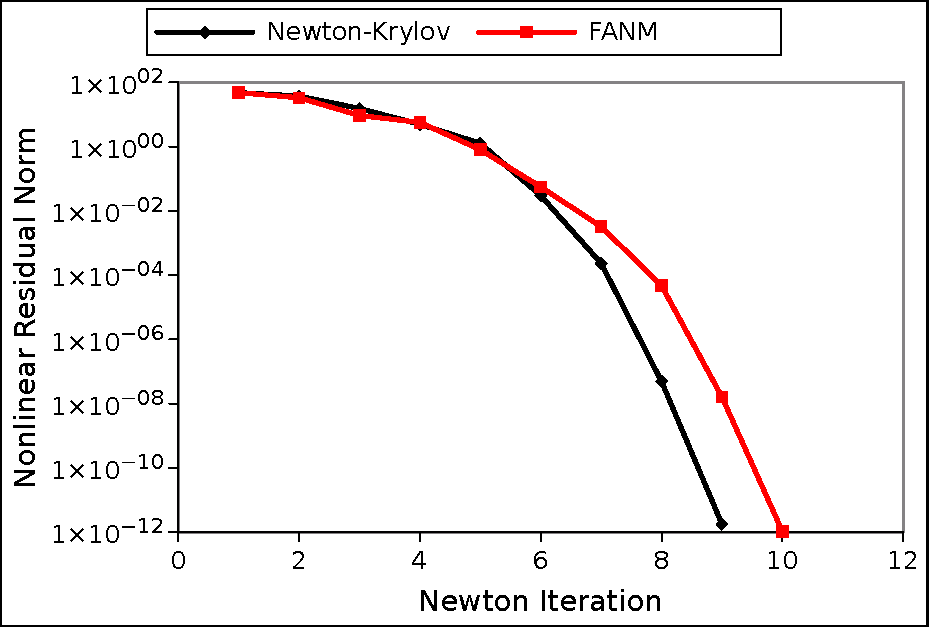
\includegraphics[width=6in]{chapters/nonlinear_problem/ra_1e5_convergence.pdf}
  \end{center}
  \caption{\textbf{Nonlinear residual norm as a function of Newton
      iteration for the \sn{1}{5} Rayleigh number case.} \textit{The
      FANM calculation required an additional nonlinear iteration to
      converge.}}
  \label{fig:ra1e5_convergence}
\end{figure}

In addition to nonlinear iterative performance, performance of the
inner linear solves is also interest. Here, we seek to maintain a
minimum number of total linear solver iterations over the course of
all nonlinear
iterations. Table~\ref{tab:convection_linear_iter_comparison} gives
the total number of GMRES iterations required to converge the problem
for the Newton-Krylov method and the total number of MCSA iterations
for the FANM method at each Rayleigh number used. For all cases, fewer
MCSA iterations were required than GMRES iterations to converge the
problem even with both solvers preconditioned with the same multigrid
package and the same parameters. For the \sn{1}{6} Rayleigh number
case this difference is most drastic with FANM requiring only 64\% of
the linear iterations required by the Newton-Krylov scheme. Even the
\sn{1}{5} Rayleigh number case that required more Newton iterations
required 5 fewer MCSA iterations to converge than GMRES iterations.

\begin{table}[h!]
  \begin{center}
    \begin{tabular}{lcc}\hline\hline
      \multicolumn{1}{l}{Rayleigh Number}& 
      \multicolumn{1}{c}{GMRES Iterations}&
      \multicolumn{1}{c}{MCSA Iterations}\\
      \hline
      \sn{1}{3} & 23 & 18 \\
      \sn{1}{4} & 23 & 17 \\
      \sn{1}{5} & 25 & 20 \\
      \sn{1}{6} & 39 & 25 \\
      %%
      \hline\hline
    \end{tabular}
  \end{center}
  \caption{\textbf{Thermal convection cavity total sum of linear
      iterations for all nonlinear iterations.} \textit{The results
      presented here were obtained from the benchmark verification
      calculations.}}
  \label{tab:convection_linear_iter_comparison}
\end{table}

Although the iterative performance of FANM is excellent for the
thermal convection cavity problem, the explicit preconditioning
strategy causes the same issues as was observed for the $SP_N$
equations in the previous
chapter. Table~\ref{tab:convection_speedup_comparison} gives the
speedup of the Newton-Krylov method over FANM. For all Rayleigh
numbers, we see a fairly constant speedup of O(400) when using
Newton-Krylov over FANM meaning that the implementation of the FANM
method used here is significantly slower. As the inexact Newton scheme
in Drekar was modified by simply swapping out the linear solver used
at each Newton step, this increased compute time is coming directly
from using MCSA as the solver and the overhead due to
preconditioning. When preconditioning overhead for the $SP_N$
equations was considered as shown by the data in
Figure~\ref{fig:spn_comparison_prec_time}, a similar speedup of
approximately two orders of magnitude was noted between the Krylov
methods and MCSA showing consistency between those results and the
fluid benchmark results. In addition, the fairly constant speedup
values as a function of the primary problem parameter show that FANM
has effectively the same time complexity as a Newton-Krylov method and
the implementation timings simply differ by a constant value.

\begin{table}[h!]
  \begin{center}
    \begin{tabular}{lcc}\hline\hline
      \multicolumn{1}{l}{Rayleigh Number}& 
      \multicolumn{1}{c}{Newton-Krylov Speedup}\\
      \hline
      \sn{1}{3} & 338 \\
      \sn{1}{4} & 336 \\
      \sn{1}{5} & 346 \\
      \sn{1}{6} & 465 \\
      %%
      \hline\hline
    \end{tabular}
  \end{center}
  \caption{\textbf{Thermal convection cavity Newton-Krylov speedup
      over FANM method.} \textit{Speedup values are rounded to the
      nearest integer. The results presented here were obtained from
      the benchmark verification calculations.}}
  \label{tab:convection_speedup_comparison}
\end{table}

\clearpage

\subsection{Lid Driven Cavity Results}
\label{subsec:lid_driven_comparison}

For the lid driven cavity benchmark, performance results were again
compared between the FANM and Newton-Krylov calculations. In this
case, the nonlinear iterative performance results as given by
Table~\ref{tab:driven_nonlinear_iter_comparison} show that the same
number of Newton iterations were required to converge the 100, 300,
and 500 Reynolds number cases while the FANM calculation with a
Reynolds number of 700 actually converged in 4 fewer iterations. The
nonlinear residual norm as a function of Newton iteration for this
case is given in Figure~\ref{fig:re700_convergence}.

This result can be explained by the fact that as given by
Table~\ref{tab:driven_mcsa_parameters}, although the preconditioner
parameters were the same for both calculations, the MCSA iteration was
pushed harder by doubling the number of histories used for the
computation at each nonlinear iteration. These extra histories
provided better convergence of the linear model at each iteration and
did not result in oversolving, thereby increasing the convergence rate
of the nonlinear model as well.

\begin{table}[h!]
  \begin{center}
    \begin{tabular}{lcc}\hline\hline
      \multicolumn{1}{l}{Reynolds Number}& 
      \multicolumn{1}{c}{Newton-Krylov Iterations}&
      \multicolumn{1}{c}{FANM Iterations}\\
      \hline
      100 & 6 & 6 \\
      300 & 9 & 9 \\
      500 & 11 & 11 \\
      700 & 14 & 10 \\
      %%
      \hline\hline
    \end{tabular}
  \end{center}
  \caption{\textbf{Lid driven cavity nonlinear iteration
      results for the performance comparison.} \textit{The results
      presented here were obtained from the benchmark verification
      calculations.}}
  \label{tab:driven_nonlinear_iter_comparison}
\end{table}

\begin{figure}[htpb!]
  \begin{center}
    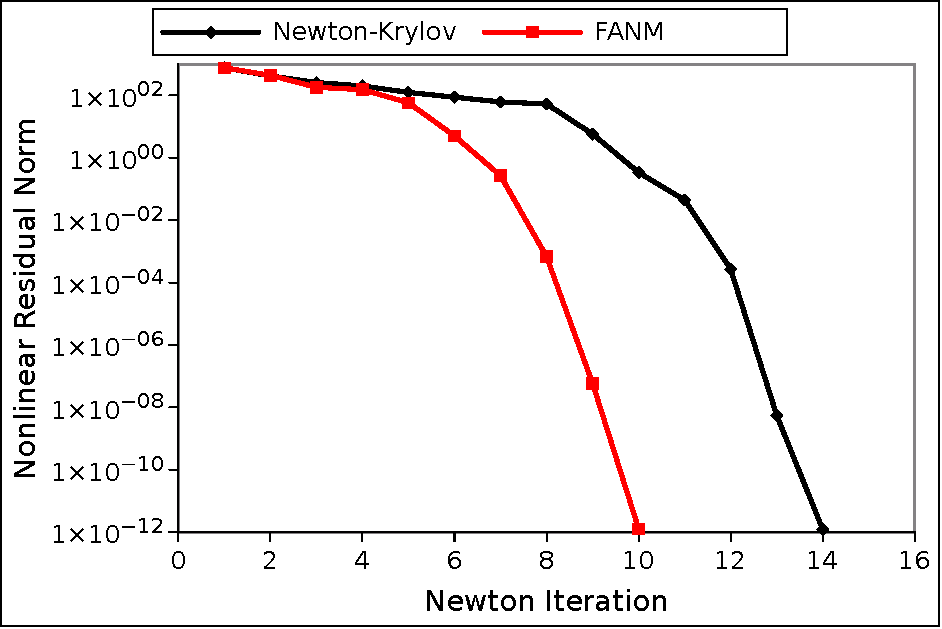
\includegraphics[width=6in]{chapters/nonlinear_problem/re700_convergence.pdf}
  \end{center}
  \caption{\textbf{Nonlinear residual norm as a function of Newton
      iteration for the 700 Reynolds number case.} \textit{The FANM
      calculation converged in 4 fewer iterations than the
      Newton-Krylov calculation.}}
  \label{fig:re700_convergence}
\end{figure}

The difficulty of this benchmark problem as compared to the thermal
convection cavity problem is readily apparent in the linear iteration
counts as given by Table~\ref{tab:driven_linear_iter_comparison}. As
the opposite of what was observed for that benchmark, lid driven
cavity results show that the linear models were significantly more
ill-conditioned, requiring many more MCSA and GMRES iterations. For
all cases except the 700 Reynolds number case, many more MCSA
iterations were required to converge with the observed GMRES iteration
count 64\% of that observed for MCSA when looking at the 100 Reynolds
number case. For the 700 Reynolds number case, fewer MCSA iterations
were observed due to the fact that 4 fewer nonlinear iterations were
performed. The average number of linear iterations per nonlinear
iteration was still much larger for the FANM calculations.

These iterative results again point out the fundamental flaw of
requiring a spectral radius of less than unity for the MCSA iteration
to converge at each Newton step. As the problem becomes more dominated
by inertial forces, the resulting linear models become increasingly
stiff and difficult to precondition. As a result, convergence requires
many more iterations than needed for the flow problem driven by
convection in the previous benchmark if convergence is achieved at
all.

\begin{table}[h!]
  \begin{center}
    \begin{tabular}{lcc}\hline\hline
      \multicolumn{1}{l}{Reynolds Number}& 
      \multicolumn{1}{c}{GMRES Iterations}&
      \multicolumn{1}{c}{MCSA Iterations}\\
      \hline
      100 & 27 & 42 \\
      300 & 35 & 52 \\
      500 & 41 & 56 \\
      700 & 21 & 14 \\
      %%
      \hline\hline
    \end{tabular}
  \end{center}
  \caption{\textbf{Lid driven cavity total sum of linear
      iterations for all nonlinear iterations.} \textit{The results
      presented here were obtained from the benchmark verification
      calculations.}}
  \label{tab:driven_linear_iter_comparison}
\end{table}

As a final comparison, the timing of both methods was again compared
with the speedup of using the Newton-Krylov solver over FANM reported
in Table~\ref{tab:driven_speedup_comparison}. The speedup values
reported here are of the same magnitude as those reported for the
thermal convection cavity problem and in agreement with those observed
for the $SP_N$ calculations. In all cases, the preconditioning
strategy must be signficantly improved to avoid these large overheads.

\begin{table}[h!]
  \begin{center}
    \begin{tabular}{lcc}\hline\hline
      \multicolumn{1}{l}{Reynolds Number}& 
      \multicolumn{1}{c}{Newton-Krylov Speedup}\\
      \hline
      100 & 299 \\
      300 & 322 \\
      500 & 288 \\
      700 & 488 \\
      %%
      \hline\hline
    \end{tabular}
  \end{center}
  \caption{\textbf{Lid driven cavity Newton-Krylov speedup
      over FANM method.} \textit{Speedup values are rounded to the
      nearest integer. The results presented here were obtained from
      the benchmark verification calculations.}}
  \label{tab:driven_speedup_comparison}
\end{table}

%%---------------------------------------------------------------------------%%
\section{Summary}
\label{sec:nonlinear_summary}

In this chapter we have developed and explored Monte Carlo synthetic
acceleration methods in the context of solutions to the nonlinear
Navier-Stokes equations. The following are the signficant observations
and findings.

\begin{itemize}
\item Forward-Automated Newton-MCSA (FANM), a new inexact Newton
  method based on Monte Carlo synthetic acceleration, has been
  developed
\item The FANM method has been incorporated into the Drekar production
  multiphysics code
\item The FANM method has been verified to produce the same solutions
  as a production Newton-Krylov method for two benchmark problems for
  the Navier-Stokes equations in different flow regimes
\item The FANM method has better iterative performance than the
  Newton-Krylov method for convection dominated problems, converging
  in fewer linear solver iterations with the same preconditioning for
  high and lower Rayleigh numbers
\item The Newton-Krylov method has better iterative performance than
  the FANM method for flow dominated by interial forces, converging in
  fewer linear solver iterations with the same preconditioning
\item The spectral radius convergence restriction on MCSA was observed
  to be a signficant hinderance by preventing solutions to forced flow
  problems at high Reynolds numbers
\item Explict algebraic preconditioning of MCSA creates FANM run times
  $O(100)$ slower than the Newton-Krylov solver
\item More Monte Carlo histories at every FANM iteration can reduce
  the number of linear and nonlinear iterations required to converge
  the problem
\end{itemize}

\chapter{Parallel Monte Carlo Synthetic \\ Acceleration Methods\ }
\label{ch:parallel_methods}
For MCSA and FANM to be viable at the production scale for nuclear
engineering applications, scalable parallel implementations of the
algorithm are required. Reviewing the literature, MCSA has yet to be
parallelized and the Neumann-Ulam Monte Carlo method on which it is
built has only been parallelized through history-level parallelism
with full domain replication \citep{alexandrov_efficient_1998}. In
order to solve large linear transport systems with MCSA, a
domain-decomposed parallel strategy is required. In the formulation of
a parallel MCSA algorithm, we recognize that the algorithm occurs in
two stages, an outer iteration performing fixed point iteration and
applying the correction, and an inner Monte Carlo solver that is
generating the correction via the adjoint or forward methods. The
parallel aspects of both these components must be
considered. Therefore, we will develop and implement parallel
algorithms for the Neumann-Ulam and MCSA methods leveraging both the
knowledge gained from the general parallel implementations of Krylov
methods reviewed in Appendix~\ref{ch:linear_problem} and modern
parallel strategies for domain decomposed Monte Carlo as developed by
the reactor physics community.

In this chapter we briefly review particle transport methods for
domain decomposed Monte Carlo. Considering a domain decomposed
Neumann-Ulam method, we derive an analytic framework based on
algebraic quantities from which to estimate aspects of its performance
when applied to neutron transport systems. We then devise a parallel
algorithm for the Neumann-Ulam method based on the multiple-set
overlapping-domain decomposition algorithm and a parallel algorithm
for the MCSA iteration that leverages the parallel Monte Carlo
algorithm and general parallel matrix-vector operations. Using
parallel solutions for the neutron diffusion problem, we verify the
correctness of the parallel algorithm and implementation by comparing
the numerical results against production Krylov methods. With the
verified implementation of the algorithm, we perform parallel scaling
studies to test its performance on a leadership class machine and
compare this performance to the production Krylov methods.

%%---------------------------------------------------------------------------%%
\section{Domain Decomposed Monte Carlo\ }
\label{sec:msod}
Large-scale problems will for reasons typically related to memory
restrictions or performance have their data partitioned such that each
parallel process owns a subset of the equations in the linear
system. Given this convention, the Neumann-Ulam Monte Carlo algorithm
must perform random walks over a domain that is decomposed and must
remain decomposed to avoid the same performance and memory
restrictions that required the domain to be decomposed. To parallelize
this algorithm, we then seek parallel Monte Carlo algorithms that
handle domain decomposition.

To motivate this problem, consider the square domain presented in
Figure~\ref{fig:ddmc_example} and on this domain we imagine a Monte
Carlo particle transport problem. If the domain were decomposed into 9
subdomains as shown, each of those subdomains and their associated
data (i.e. cross sections) could be owned by a different parallel
process in the computation. In Figure~\ref{fig:ddmc_example}, the
tracks of 3 particles that are born in the center subdomain are
shown. In this example, particle A is first transported from the
center domain to the domain directly to the left. Before the
scattering event in the new domain may be processed, particle A must
be communicated between between the two parallel processes that own
those domains. For any given particle in the transport simulation,
this communication event may hardly occur during the lifetime of the
particle (particle B), or may occur many times (particle C) depending
on the problem parameters and the random path in phase space taken by
the particle. Scalable parallel algorithms for domain decomposed Monte
Carlo are those that handle this domain-to-domain communication of
particles effectively and balance it with the on-process computations
for particle interactions, tallies, response calculations, and other
simulation requirements.
\begin{figure}[t!]
  \begin{center}
    \scalebox{1.5}{
      \input{chapters/parallel_mc/ddmc_example.pdftex_t} }
  \end{center}
  \caption{\textbf{Domain decomposed Monte Carlo transport example
      illustrating how domain decomposition requires parallel
      communication of particles.} \textit{If a particle crosses a
      domain boundary it must be communicated to the next domain in
      its path.}}
  \label{fig:ddmc_example}
\end{figure}

For a domain decomposed Neumann-Ulam method, the situation is very
much the same where instead the transport process is now discrete and
the "physics" of the transport process is the Monte Carlo game with
probabilities and weights described by
Eq~(\ref{eq:neumann_ulam_decomposition}) for the given linear
problem. Figure~\ref{fig:ddnu_example} gives the domain decomposed
Neumann-Ulam analog of particle transport problem in
Figure~\ref{fig:ddmc_example}. Imagine in this problem that we are
solving for the monoenergetic scalar neutron flux as in the model
diffusion problem presented in Appendix~\ref{chap:diffusion_problem}.
In this problem, the solution has only a spatial dependence and
therefore each point in the mesh corresponds to an equation in the
resulting linear system. In Figure~\ref{fig:ddnu_example}, the domain
has now been discretized by this mesh and again decomposed into 9
subdomains, each owning a piece of the mesh and therefore the
corresponding equations in the linear system. As we play the Monte
Carlo game presented in Chapter~\ref{ch:stochastic_methods}, the
discretization and resulting Neumann-Ulam decomposition of the problem
describes how each state in the system is coupled to the other states
in the system through the set of equations that form the linear
system. This coupling is then responsible for the discrete random walk
that each history takes as shown in this example. As discrete states
(or rows in the linear system) that do not exist in the local domain
are reached during the random walk by stochastic histories, the
histories must be communicated to the subdomain that does own the
discrete state in an analogous fashion to the particles in the
previous example.
\begin{figure}[t!]
  \begin{center}
    \scalebox{1.5}{
      \input{chapters/parallel_mc/ddnu_example.pdftex_t} }
  \end{center}
  \caption{\textbf{Domain decomposed Neumann-Ulam example illustrating
      how domain decomposition requires parallel communication of
      histories.} \textit{Each mesh point corresponds to an equation
      in the linear system and the coupling among equations is
      described by the discretization of the problem.}}
  \label{fig:ddnu_example}
\end{figure}

To further motivate using a parallel algorithm similar to particle
transport methods, again consider history A in
Figure~\ref{fig:ddnu_example}. This history begins in the center
subdomain and through the course of transitioning through states in
the system arrives at a state that exists in the subdomain directly to
the left of the center subdomain. History A must then be communicated
from the center subdomain to the subdomain immediately to the left to
continue the random walk. As with the particle transport system, we
may find that histories in a domain decomposed Neumann-Ulam method are
only communicated a few times (history B) if at all, or they may be
communicated many times (history C) depending on the discretization
and the outcome of the Monte Carlo game. In identical fashion to the
particle transport problem, a domain decomposed Neumann-Ulam method
has the same communication requirements with all histories in both
examples requiring the same parallel operations. The amount of
communication of histories from domain to domain will be the primary
factor in the parallel scalability of the algorithm. In the next
section, the number of histories communicated in a given problem will
be quantified analytically for a simple model problem.

\clearpage

%%---------------------------------------------------------------------------%%
\section{Analytic Framework for Domain-Decomposed Monte Carlo\ }
\label{sec:analytic_framework}
To date, parallel Neumann-Ulam methods have been limited to full
domain replication with parallelism exploited through individual
histories \citep{alexandrov_efficient_1998} and in this chapter we
will exploit particle transport algorithms to alleviate this. To
accomplish this, we recognize from the literature that stochastic
histories must be transported from domain to domain as the simulation
progresses and they transition to states that are not in the local
domain. Because we have chosen a domain decomposition strategy in a
parallel environment, this means that communication of these histories
must occur between compute nodes owning neighboring pieces of the
global domain. We wish to characterize this communication not only
because communication is in general expensive, but also because these
nearest-neighbor communication sequences, specifically, have poor
algorithmic strong scaling \citep{gropp_high-performance_2001} in much
the same way as a parallel matrix-vector multiply
operation. Therefore, we desire a framework to provide a simple,
analytic theory based on the properties of the transport system that
will allow for estimates of the domain decomposed behavior of the
Neumann-Ulam method in terms of the amount of information that must be
communicated.

When solving problems where the linear operator is symmetric, a host
of analytic techniques exist based on the eigenvalue spectrum of the
operator that characterize their behavior in the context of
deterministic linear solvers. Using past work, these techniques are
adapted to the domain decomposed Neumann-Ulam method using the
one-speed, two-dimensional neutron diffusion equation and spatial
discretization presented in Appendix~\ref{chap:diffusion_problem} as a
model transport problem. Using the linear system generated by the
discretization of the model problem, we use a spectral analysis to
generate analytic relations for the eigenvalues of the operator based
on system parameters. Using the eigenvalue spectra, we then build
relationships to characterize the transport of stochastic histories in
a decomposed domain and the fraction of histories that leak from a
domain and will therefore have to be communicated. Finally, we compare
these analytic results to numerical experiments conducted with the
model transport problem.

\clearpage

\subsection{Spectral Analysis }
\label{subsec:spectral_analysis}
The convergence of the Neumann series in
Eq~(\ref{eq:adjoint_neumann_series}) approximated by the Monte Carlo
solver is dependent on the eigenvalues of the iteration matrix. We
will compute these eigenvalues by assuming eigenfunctions of the form
\citep{leveque_finite_2007}:
\begin{equation}
  \Phi_{p,q}(x,y) = e^{2 \pi \imath p x} e^{2 \pi \imath q y}\:,
  \label{eq:eigenfunction_form}
\end{equation}
where different combinations of $p$ and $q$ represent the different
eigenmodes of the solution. As these are valid forms of the solution,
then the action of the linear operator on these eigenfunctions will
yield the eigenvalues of the matrix as they exist on the unit circle
in the complex plane.

For the model problem, we first compute the eigenvalues for the
diffusion operator $\ve{D}$ by applying the operator to the
eigenfunctions and noting that $x=ih$ and $y=jh$:
\begin{multline}
  \ve{D}\Phi_{p,q}(x,y) = \lambda_{p,q}(\ve{D})
  =\\ -\frac{D}{6h^2}\Big[4 e^{-2 \pi \imath p h} + 4 e^{2 \pi \imath
      p h} + 4 e^{-2 \pi \imath q h} + 4 e^{2 \pi \imath q h} + e^{-2
      \pi \imath p h} e^{-2 \pi \imath q h} \\ + e^{-2 \pi \imath p h}
    e^{2 \pi \imath q h} + e^{2 \pi \imath p h} e^{-2 \pi \imath q h}
    + e^{2 \pi \imath p h} e^{2 \pi \imath q h} - 20\Big] + \Sigma_a
  \:.
  \label{eq:deriv_diff_1}
\end{multline}
Using Euler's formula, we can collapse the exponentials to
trigonometric functions:
\begin{equation}
  \lambda_{p,q}(\ve{D}) = -\frac{D}{6h^2}[ 8 \cos(\pi p h) + 8
    \cos(\pi q h) + 4 \cos(\pi p h) \cos(\pi q h) - 20] + \Sigma_a\:.
  \label{eq:deriv_diff_2}
\end{equation}

As Eq~(\ref{eq:diffusion_eq}) is diagonally dominant, point Jacobi
preconditioning as outlined in
\S~\ref{subsec:stochastic_preconditioning} is sufficient to reduce the
spectral radius of the iteration matrix below unity and therefore
ensure convergence of the Neumann series. Applying this
preconditioner, we are then solving the following diffusion system:
\begin{equation}
  \ve{M}^{-1} \ve{D} \boldsymbol{\phi} = \ve{M}^{-1} \ve{s}\:.
  \label{eq:precond_diffsion}
\end{equation}
The operator $\ve{M}^{-1} \ve{D}$ is merely the original diffusion
operator with each row scaled by the diagonal component. As we have
defined a homogeneous domain, the scaling factor, $\alpha$, is the
same for all rows in the operator and defined as the $\phi_{i,j}$
coefficient from Eq~(\ref{eq:fd_system}):
\begin{equation}
  \alpha = \Bigg[\frac{10 D}{3 h^2} + \Sigma_a\Bigg]^{-1}\:.
  \label{eq:jacobi_scaling}
\end{equation}
Using this coefficient, we then have the following spectrum of
preconditioned eigenvalues:
\begin{equation}
  \lambda_{p,q}(\ve{M}^{-1} \ve{D}) = \alpha \lambda_{p,q}(\ve{D})\:.
  \label{eq:preconditioned_eigenvalues}
\end{equation}

The spectral radius of the iteration matrix is obtained by seeking its
largest eigenvalue. As with the diffusion operator, we can use the
same analysis techniques to find the eigenvalues for the iteration
matrix. We use a few simplifications by noting that if the Jacobi
preconditioned iteration matrix is $\ve{H} = \ve{I} -
\ve{M}^{-1}\ve{D}$, the we except all terms on the diagonal of the
iteration matrix to be zero such that we have the following stencil:
\begin{multline}
  \ve{H}\boldsymbol{\phi} = \frac{\alpha D}{6h^2}\Big[4 \phi_{i-1,j} +
    4 \phi_{i+1,j} + 4 \phi_{i,j-1} + 4 \phi_{i,j+1}
    +\\ \phi_{i-1,j-1} + \phi_{i-1,j+1} + \phi_{i+1,j-1} +
    \phi_{i+1,j+1}\Big]\:.
  \label{eq:iteration_stencil}
\end{multline}
Inserting the eigenfunctions defined by
Eq~(\ref{eq:eigenfunction_form}) we get:
\begin{multline}
  \lambda_{p,q}(\ve{H}) = \frac{\alpha D}{6h^2}\Big[4 e^{-2 \pi \imath p
      h} + 4 e^{2 \pi \imath p h} + 4 e^{-2 \pi \imath q h} + 4 e^{2
      \pi \imath q h} + e^{-2 \pi \imath p h} e^{-2 \pi \imath q h}
    \\ + e^{-2 \pi \imath p h} e^{2 \pi \imath q q} + e^{2 \pi \imath
      p h} e^{-2 \pi \imath q h} + e^{2 \pi \imath p h} e^{2 \pi
      \imath q h}\Big]\:,
  \label{eq:iteration_deriv}
\end{multline}
which simplifies to:
\begin{equation}
  \lambda_{p,q}(\ve{H}) = \frac{\alpha D}{6h^2}[ 8 \cos(\pi p h) + 8
    \cos(\pi q h) + 4 \cos(\pi p h) \cos(\pi q h)]\:,
  \label{eq:iteration_spectrum}
\end{equation}
giving the eigenvalue spectrum for the Jacobi preconditioned iteration
matrix. To find the maximum eigenvalue,
Eq~(\ref{eq:preconditioned_eigenvalues}) is plotted as a function of
$p$ with $p=q$ in Figure~\ref{fig:diffusion_spectrum} for various
values of $\Sigma_a$.
\begin{figure}[t!]
  \begin{center}
    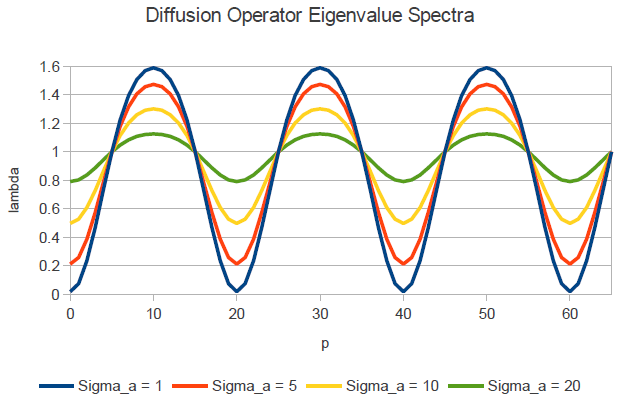
\includegraphics[width=5in,clip]{chapters/parallel_mc/diffusion_spectrum.png}
  \end{center}
  \caption{\textbf{Eigenvalue spectra for the diffusion equation.}}
  \label{fig:diffusion_spectrum}
\end{figure}
We find that the maximum eigenvalue exists when $p=q=0$, giving the
following for the spectral radius of the Jacobi preconditioned
iteration matrix:
\begin{equation}
  \rho(\ve{H}) = \frac{10 \alpha D}{3 h^2}\:.
  \label{eq:iteration_radius}
\end{equation}

\clearpage 

\subsection{Neumann Series Convergence }
\label{subsec:neumann_convergence}
As outlined in \S\ref{sec:mc_preliminaries}, the adjoint Monte Carlo
method is effectively an approximation to a stationary method. In the
adjoint Neumann-Ulam method, $k$ iterations, equivalent to $k$
applications of the iteration matrix, are approximated by a random
walk of average length $k$ to yield the summation in
Eq~(\ref{eq:adjoint_neumann_solution})
\citep{dimov_new_1998,danilov_asymptotic_2000}. This random walk
length, or the number of transitions before the termination of a
history (either by the weight cutoff, absorption, or exiting the
global domain) is therefore approximately the number of stationary
iterations required to converge to the specified tolerance. In the
case of the adjoint Neumann-Ulam method, no such tolerance exists,
however, we have specified a weight cutoff, $W_c$, that determines
when low-weight histories will be prematurely terminated as their
contributions are deemed minute. After $k$ iterations, a stationary
method is terminated as the error has reached some fraction,
$\epsilon$, of the initial error:
\begin{equation}
  ||\ve{e}^{k}||_2 = \epsilon ||\ve{e}^0||_2\:.
  \label{eq:linear_k_iter_norm4}
\end{equation}
Per Eq~(\ref{eq:linear_k_iter_norm3}), we see that this fraction is
equivalent to $\epsilon = \rho(\ve{H})^k$. For the adjoint
Neumann-Ulam method, if we take this fraction to be the weight cutoff,
a measure of how accurately the contributions of a particular history
to the solution are tallied, we then have the following relationship
for $k$:
\begin{equation}
  k = \frac{ \log(W_c) }{ \log( \rho(\ve{H}) ) }\:.
  \label{eq:analytic_k}
\end{equation}
This then gives us a means to estimate the length of the random walks
that will be generated from a particular linear operator based on the
eigenvalues of its iteration matrix (independent of the linear
operator splitting chosen) and based on the weight cutoff parameter
used in the Neumann-Ulam method.

\subsection{Domain Leakage Approximations }
\label{subsec:domain_leak_approx}
In a domain decomposed situation, not all histories will remain within
the domain they started in and must instead be communicated. This
communication, expected to be expensive, was analyzed by Siegel and
colleagues for idealized, load balanced situations for full nuclear
reactor core Monte Carlo neutral particle simulations
\citep{siegel_analysis_2012}.  To quantify the number of particles
that leak out of the local domain they define a leakage fraction,
$\Lambda$, as:
\begin{equation}
  \Lambda = \frac{average\ \#\ of\ particles\ leaving\ local\ domain}
          {total\ of\ \#\ of\ particles\ starting\ in\ local\ domain}\:.
          \label{eq:leakage_fraction}
\end{equation}
For their studies, Siegel and colleagues assumed that the value of
$\Lambda$ was dependent on the total cross section of the system via
the Wigner rational approximation. Outlined more thoroughly by Hwang's
chapter in \citep{azmy_nuclear_2010}, we will use both the Wigner
rational approximation and the mean chord approximation as a means to
estimate the leakage fraction.

In the case of domain decomposed linear systems, we can use diffusion
theory to estimate the optical thickness of a domain in the
decomposition and the corresponding leakage fraction in terms of
properties of the linear operator and the discretization. To begin we
must first calculate the mean distance a Monte Carlo history will move
in the grid by computing the mean squared distance of its movement
along the chord of length $l$ defined across the domain. After a
single transition a history will have moved a mean squared distance
of:
\begin{equation}
  \langle \bar{r_1^2} \rangle = (n_s h)^2\:,
  \label{eq:step_1_length}
\end{equation}
where $h$ is the size of the discrete grid elements along the chord
and $n_s$ is the number of grid elements a history will move on
average every transition. For our diffusion model problem, $n_s$ would
equate to the expected number of states in the $i$ (or $j$ as the problem is
symmetric) direction that a history will move in a single
transition and is dependent on the stencil used for the
discretization. After $k$ transitions in the random walk, the history
will have moved a mean squared distance of:
\begin{equation}
  \langle \bar{r_k^2} \rangle = k (n_s h)^2\:.
  \label{eq:step_k_length}
\end{equation}
If our chord is of length $l$ and there are $n_i$ grid elements (or
states to which a history may transition) along that chord, then $h =
l / n_i$ giving:
\begin{equation}
  \langle \bar{r_k^2} \rangle = k \Bigg(\frac{n_s l}{n_i}\Bigg)^2\:.
  \label{eq:step_k_length_sub}
\end{equation}
From diffusion theory, we expect the average number of interactions
along the chord to be:
\begin{equation}
  \tau = \frac{l}{2 d \sqrt{\langle \bar{r_k^2} \rangle}}\:,
  \label{eq:optical_thickness_1}
\end{equation}
where $d$ is the dimensionality of the problem and $\sqrt{\langle
  \bar{r_k^2} \rangle}$ is effectively the mean free path of the Monte
Carlo history in the domain. We can readily interpret $\tau$ to be the
\textit{effective optical thickness} of a domain of length
$l$. Inserting Eq~(\ref{eq:step_k_length_sub}) we arrive at:
\begin{equation}
  \tau = \frac{n_i}{2 d n_s \sqrt{k}}\:,
  \label{eq:optical_thickness_2}
\end{equation}
which if expanded with Eq~(\ref{eq:analytic_k}) gives us the final
relation for the effective optical thickness:
\begin{equation}
  \tau = \frac{n_i}{2 d n_s}
  \sqrt{\frac{\log(\rho(\ve{H}))}{\log(W_c)}}\:.
  \label{eq:optical_thickness_3}
\end{equation}

For optically thin domains, we expect that most histories will be
communicated, while optically thick domains will leak the fraction of
histories that did not interact within. Using the optical thickness
defined in Eq~(\ref{eq:optical_thickness_3}), we can then complete the
leakage approximations by defining the bounds of $\tau \rightarrow 0,
\Lambda \rightarrow 1$ and $\tau \rightarrow \infty, \Lambda
\rightarrow \tau^{-1}$.  With these bounds we can then define the
leakage fraction out of a domain for the adjoint Neumann-Ulam method
using the Wigner rational approximation:
\begin{equation}
  \Lambda = \frac{1}{1+\tau}\:,
  \label{eq:wigner_domain_leakage}
\end{equation}
and using the mean-chord approximation:
\begin{equation}
  \Lambda = \frac{1-e^{-\tau}}{\tau}\:.
  \label{eq:mean_chord_domain_leakage}
\end{equation}
Here, the leakage fraction is explicitly bound to the eigenvalues of
the iteration matrix, the size of the domain, the content of the
discretization stencil, and the weight cutoff selected to terminate
low weight histories.

\subsection{Numerical Experiments }
\label{subsec:numerical_experiments}
To test the relationships developed by the spectral analysis, we form
two simple numerical experiments using the diffusion model problem:
one to measure the length of the random walks as a function of the
iteration matrix eigenvalues, and one to measure the domain leakage
fraction as a function of the iteration matrix eigenvalues and the
discretization properties. Before doing this, we verify our
computation of the spectral radius of the iteration matrix by
numerically computing the largest eigenvalue of the diffusion operator
using an iterative eigenvalue solver. For this verification, a $100
\times 100$ square grid with $h=0.01$, $h=0.1$, and $h=1.0$ and the
absorption cross varied from 0 to 100 while the scattering cross
section was fixed at unity. Figure~\ref{fig:measured_spec_rad} gives
the measured spectral radius of the iteration matrix and the computed
spectral radius for the preconditioned diffusion operator using
Eq~(\ref{eq:iteration_radius}) as function of the absorption to
scattering ratio $(\Sigma_a / \Sigma_s)$. Excellent agreement was
observed between the analytic and numerical results with all data
points computed within the tolerance of the iterative eigenvalue
solver.
\begin{figure}[t!]
  \begin{spacing}{1.0}
    \begin{center}
      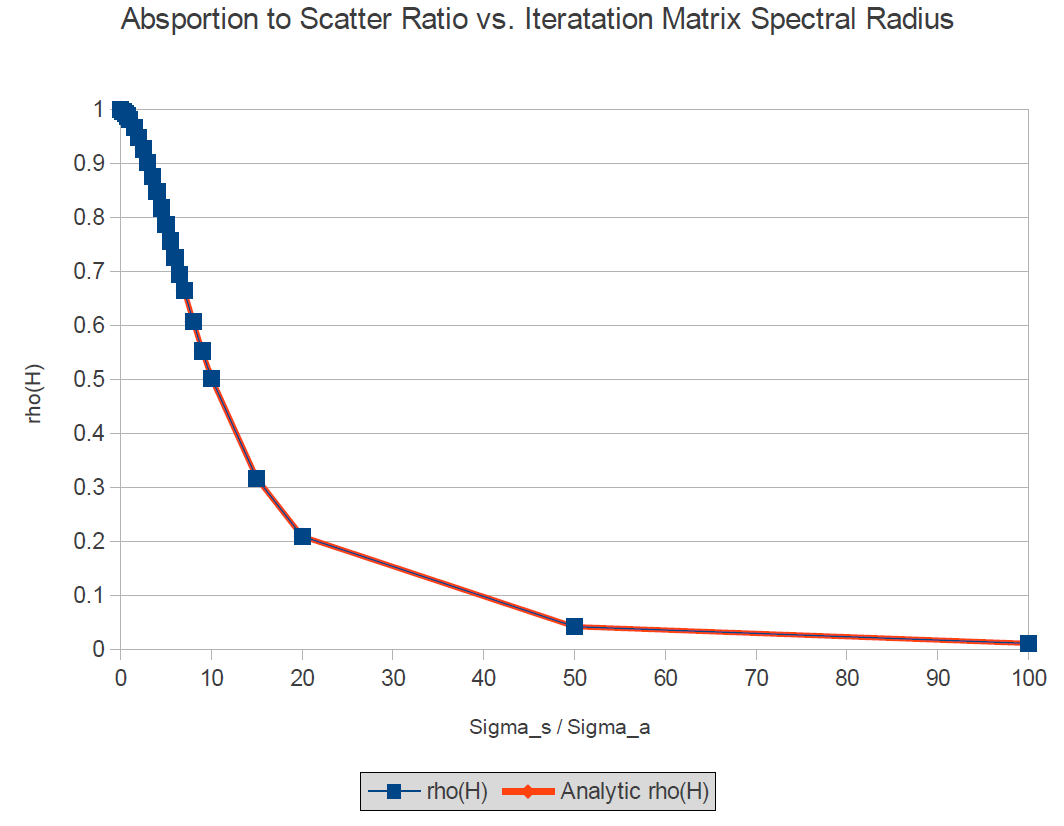
\includegraphics[width=5in,clip]{chapters/parallel_mc/measured_spec_rad.png}
    \end{center}
    \caption{\textbf{Measured and analytic preconditioned diffusion
        operator spectral radius as a function of the absorption cross
        section to scattering cross section ratio.} \textit{Values of
        $h=0.01$, $h=0.1$, and $h=1.0$ were used. The red data was
        computed numerically by an eigensolver while the black dashed
        data was generated by Eq~(\ref{eq:iteration_radius}).}}
    \label{fig:measured_spec_rad}
  \end{spacing}
\end{figure}

\subsubsection{Random Walk Length }
\label{subsubsec:walk_length}
With the eigenvalue derivations verified, we can go about setting up
an experiment to measure the length of the random walks generated by
the adjoint Neumann-Ulam solver. To do this, we again use a $100
\times 100$ square grid with $h=0.1$ and the absorption cross varied
from 0 to 100 while the scattering cross section was fixed at
unity. Three weight cutoff values of \sn{1}{-2}, \sn{1}{-4}, and
\sn{1}{-8} were used with 10,000 histories generated by a point source
of strength 1 in the center of the domain. For each of the histories,
the number of transitions made was tallied to provide an effective
value of $k$ for each history. This value was then averaged over all
histories to get a measured value of $k$ for the particular
operator. On the left, Figure~\ref{fig:measured_length} presents these
measurements as well as the analytic result computed by
Eq~(\ref{eq:analytic_k}) as a function of the iteration matrix
spectral radius, $\rho(\ve{H})$. On the right,
Figure~\ref{fig:measured_length} gives the relative difference between the
predicted and observed results. We note good qualitative agreement
between the measured and analytic results. However, we observe a
larger relative difference for both long and short random walks.
\begin{figure}[t!]
  \begin{spacing}{1.0}
    \begin{center}
      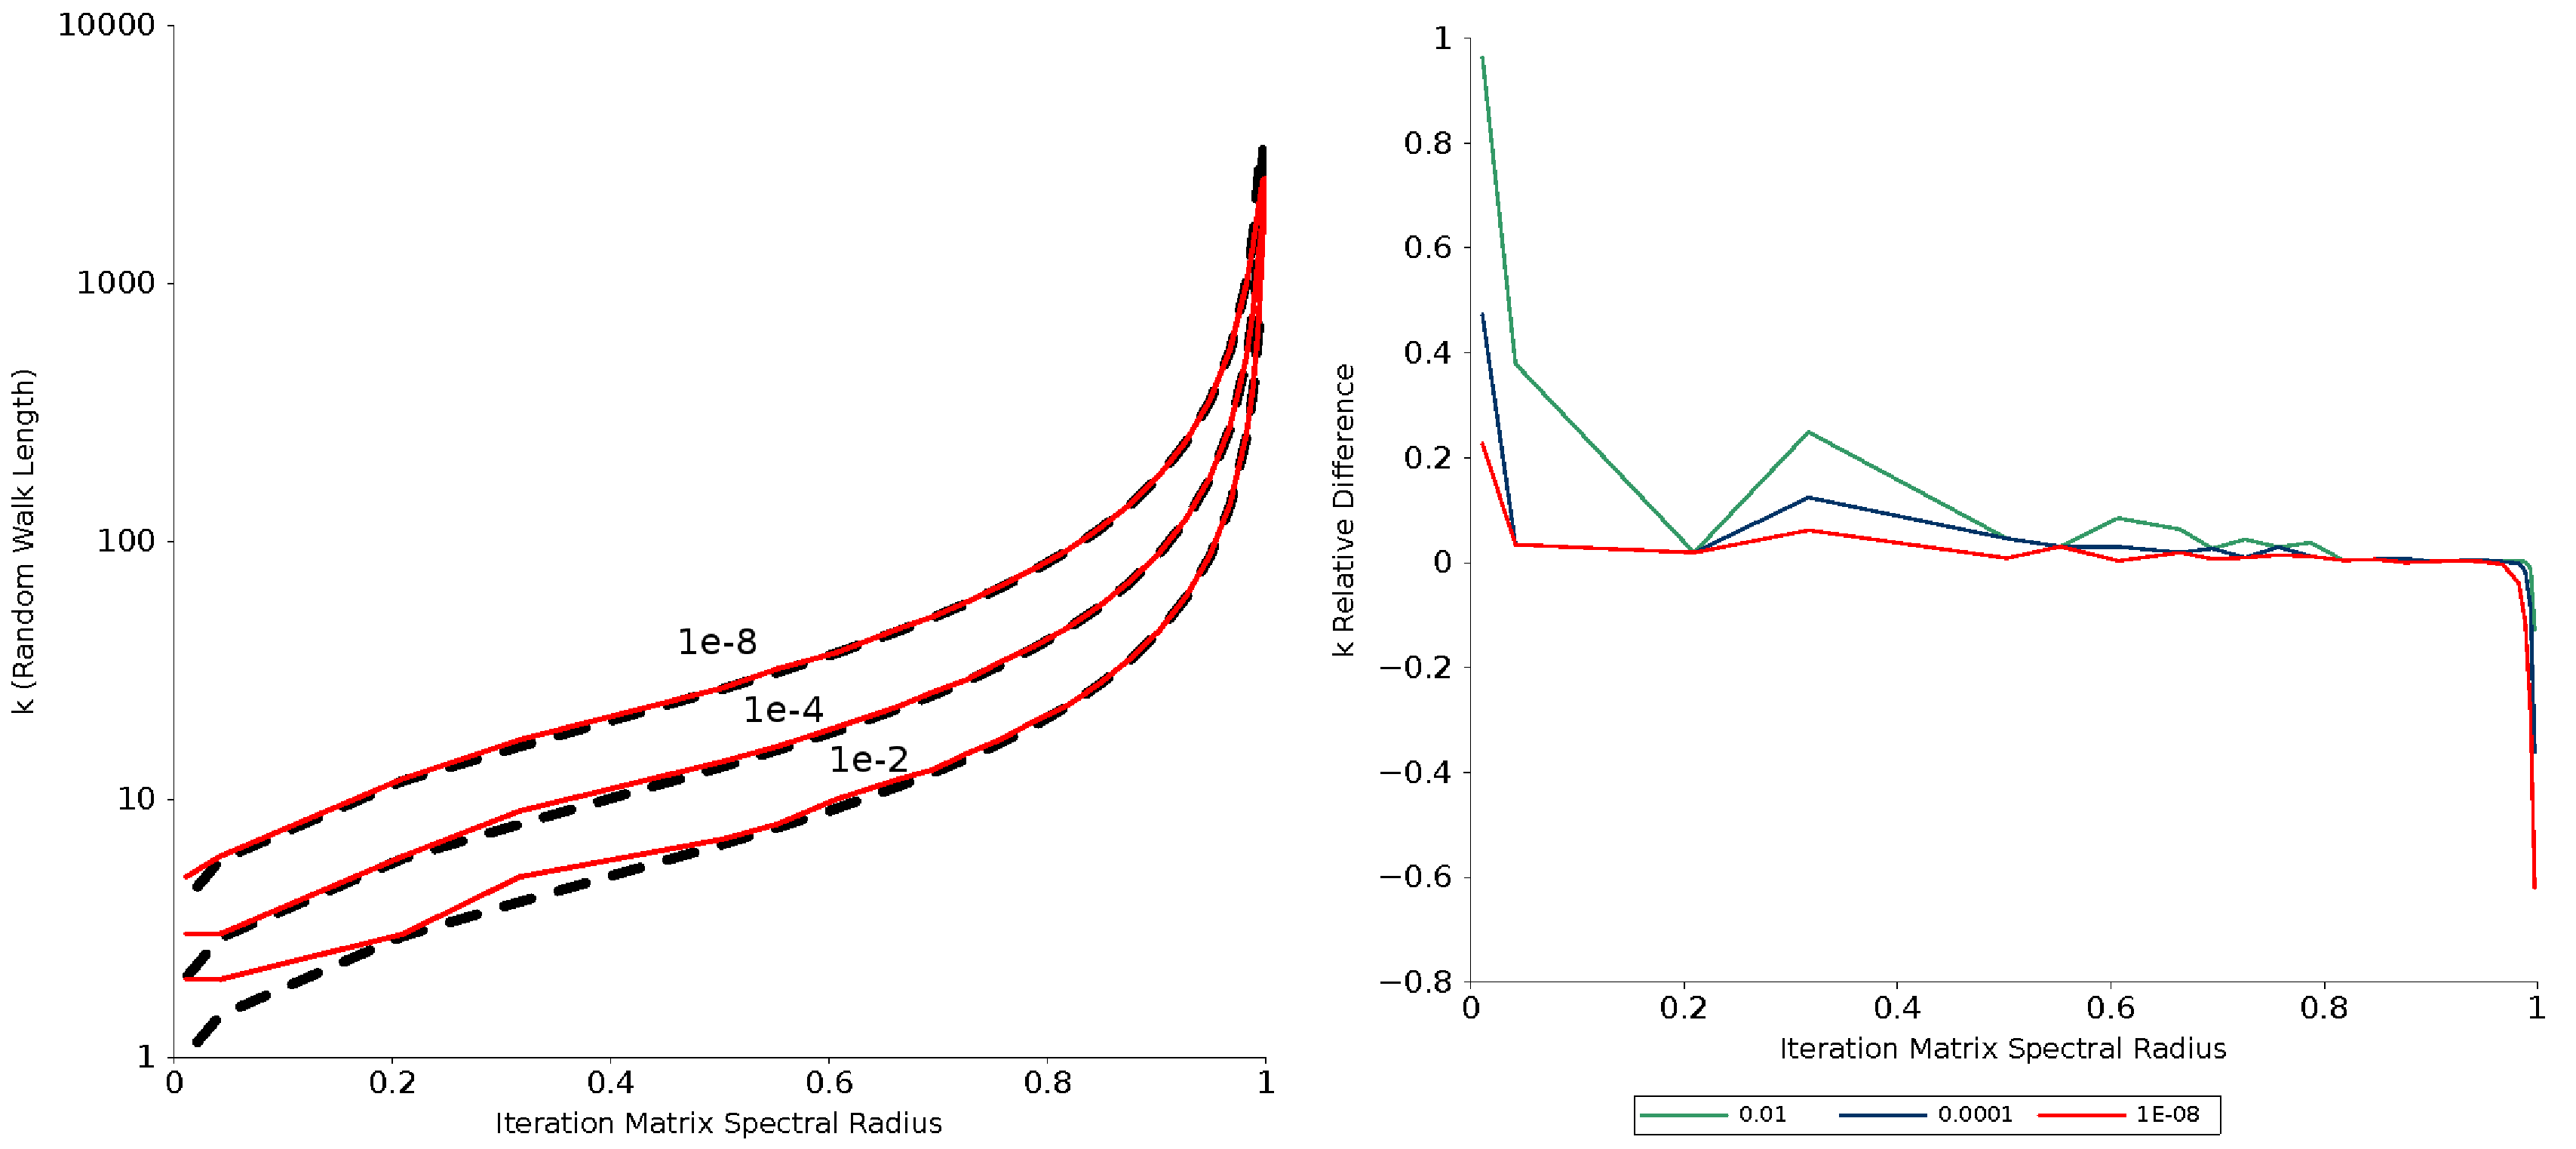
\includegraphics[width=6.0in,clip]{chapters/parallel_mc/measured_length_2.pdf}
    \end{center}
    \caption{\textbf{Measured and analytic random walk length as a
        function of the iteration matrix spectral radius.} \textit{The
        weight cutoff was varied with \sn{1}{-2}, \sn{1}{-4}, and
        \sn{1}{-8}. In the left plot, the red data was computed
        numerically by an adjoint Neumann-Ulam implementation while
        the black dashed data was generated by
        Eq~(\ref{eq:analytic_k}). In the right plot, the relative
        difference between the predicted and measured results is
        presented for each weight cutoff.}}
    \label{fig:measured_length}
  \end{spacing}
\end{figure}

\subsubsection{Domain Leakage }
\label{subsubsec:domain_leakage}
Finally, we seek to measure the leakage from a domain in a domain
decomposed Monte Carlo calculation and assess the quality of our
analytic relation for the optical thickness of a domain and the
associated leakage approximations. For this experiment, a square grid
with $h=0.1$ was decomposed into 9 square domains, 3 in each cardinal
direction with measurements occurring in the central domain without
boundary grid points. For the cross sections, the absorption cross
section was varied from 1 to 100 while the scattering cross
section was set to zero to create a purely absorbing environment
with weight cutoff of \sn{1}{-4}. The optical thickness of these
domains will vary as a function of the absorption cross section if
the other parameters are fixed. 

To compute the optical thickness, along with the spectral radius as
given by Eq~(\ref{eq:iteration_radius}), we also need the parameters
$n_i$ and $n_s$ which respectively describe the typical domain length
and the average number of states moved along that typical length per
history transition. For our grid above, the domains are varied in size
with $50 \times 50$, $100 \times 100$, and $200 \times 200$ cells
giving $n_i=50$, $n_i=100$, and $n_i=200$ grid points or states along
the typical length of the domain respectively. Looking at the
Laplacian stencil in Eq~(\ref{eq:nine_point_stencil}), we see that all
history transitions will only move a single state in either the $i$ or
$j$ directions due to the symmetry of the problem. Furthermore, if we
choose the $i$ direction, not all states we will transition to will
move the history in that direction. Therefore, we look to the
definition of the iteration matrix in Eq~(\ref{eq:iteration_stencil})
and the definition of the adjoint probability matrix in
Eq~(\ref{eq:adjoint_probability}) to estimate the $n_s$ parameter. For
a particular transition starting at state $(i,j)$, 6 of the 8 possible
new states in the stencil move the history in $i$ direction with
relative coefficients of 4 for moving in the $(\pm i,0)$ direction and
of 1 for moving in the $(\pm i,\pm j)$. These coefficients dictate the
frequency those states are visited relative to the others. For those 6
states we can visit along the typical length, their sum is 12 out of
the total 20 for the coefficients for all possible states with their
ratio giving $n_s = \frac{3}{5}$.

To compute the leakage fraction numerically, \sn{3}{5} histories were
sampled from a uniform source of strength unity over the global
domain. At the start of a stage of histories, the number of histories
starting in the center domain was computed and as the stage
progressed, the number of histories that exited that domain was
tallied with the ratio of the two numbers providing a numerical
measure for the leakage fraction. Figure~\ref{fig:measured_leakage}
gives the domain leakage measurements for the domain in the center of
the global grid as well as the analytic result computed by
Eqs~(\ref{eq:wigner_domain_leakage}) and
(\ref{eq:mean_chord_domain_leakage}) as a function of the iteration
matrix spectral radius.
\begin{figure}[t!]
  \begin{spacing}{1.0}
    \begin{center}
      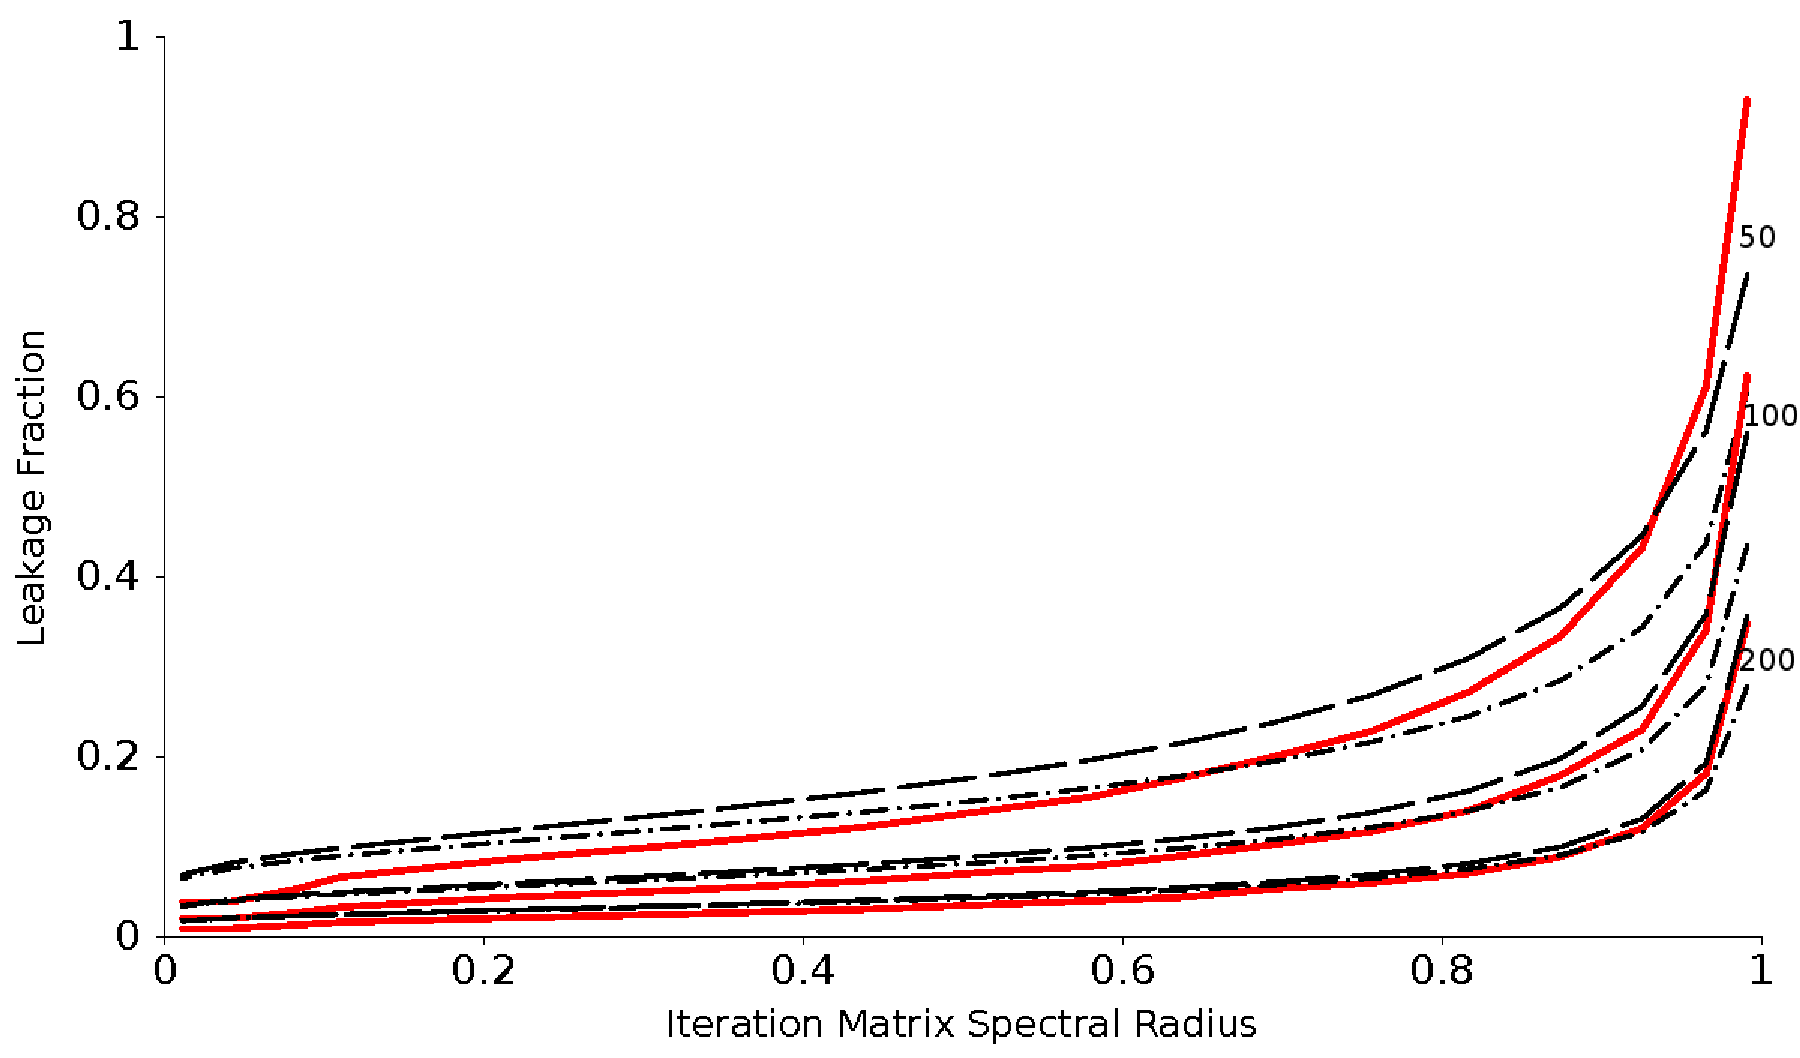
\includegraphics[width=6.0in,clip]{chapters/parallel_mc/leakage_variation_2.pdf}
    \end{center}
    \caption{\textbf{Measured and analytic domain leakage as a
        function of the iteration matrix spectral radius.} \textit{To
        test the behavior with respect to domain size, $n_i=50$,
        $n_i=100$,and $n_i=200$ were used. The red data was computed
        numerically by a domain-decomposed adjoint Neumann-Ulam
        implementation, the black dashed data was generated by
        Eq~(\ref{eq:mean_chord_domain_leakage}) using the mean-chord
        approximation, and the dashed-dotted black data was generated
        by Eq~(\ref{eq:wigner_domain_leakage}) using the Wigner
        rational approximation.}}
    \label{fig:measured_leakage}
  \end{spacing}
\end{figure}
Again, we note good qualitative agreement between the measured and
analytic quantities but we begin to see the limits of the leakage
approximations. 

To compare the quality of the two approximations, the absolute
difference between the computed leakage fraction and that generated by
the Wigner rational and mean chord approximations is plotted in
Figure~\ref{fig:leakage_error} for all domain sizes tested.
\begin{figure}[t!]
  \begin{spacing}{1.0}
    \begin{center}
      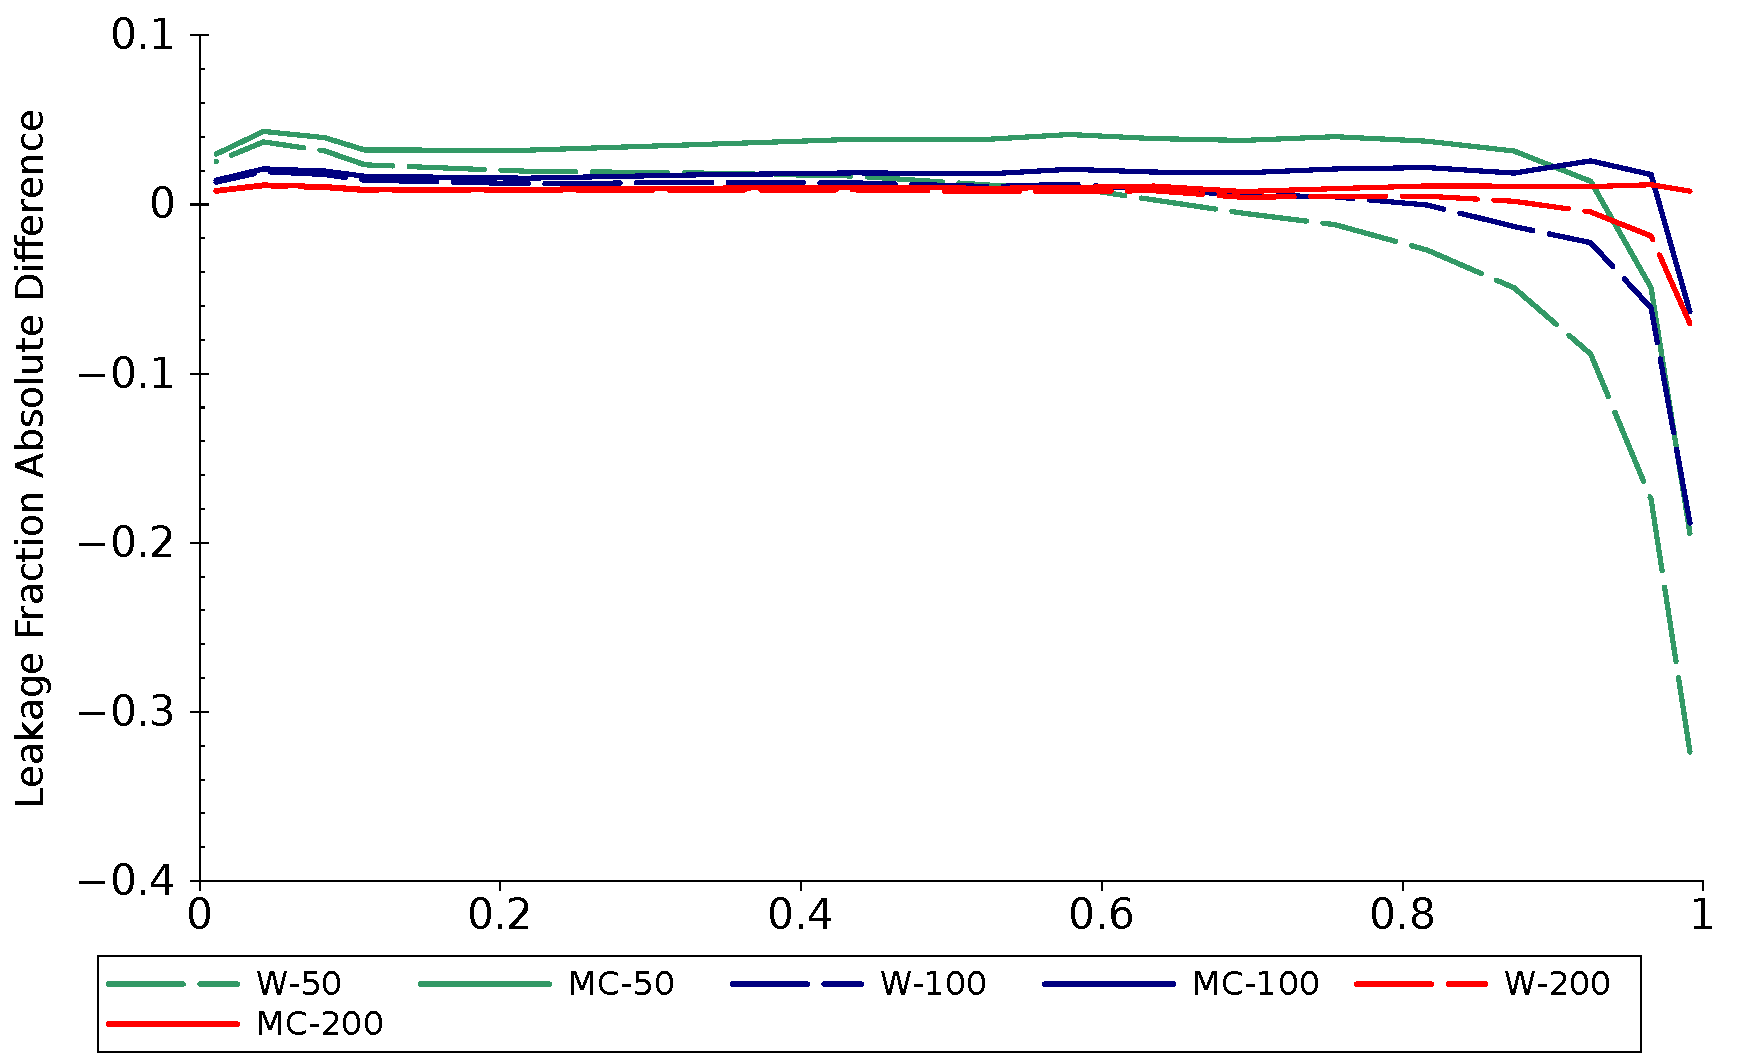
\includegraphics[width=6.0in,clip]{chapters/parallel_mc/leakage_error_2.pdf}
    \end{center}
    \caption{\textbf{Measured and analytic domain leakage absolute
        difference as a function of the iteration matrix spectral radius.}
      \textit{To test the behavior with respect to domain size,
        $n_i=50$ (green), $n_i=100$ (blue), and $n_i=200$ (red) were
        used. The dashed lines represent the difference using the Wigner
        rational approximation while the solid lines represent the
        difference using the mean-chord approximation.}}
    \label{fig:leakage_error}
  \end{spacing}
\end{figure}
From these difference results, the mean chord approximation is shown to
have a lower difference for ill-conditioned systems as compared to the
Wigner approximation while the Wigner approximation produces less
difference for more well-conditioned systems. We also note that for the
optically thick domains, the difference is likely corresponded to that
observed in Figure~\ref{fig:measured_length} for the $k$ parameter
while the large relative difference in $k$ for optically thin domains does
not affect the approximation significantly. In general, the mean chord
approximation is a better choice to estimate the leakage fraction in a
domain from the adjoint Neumann-Ulam method and except for a single
data point with $n_i=50$, the mean chord approximation yielded leakage
fractions within 0.05 of the measured results. As the domain becomes
more optically thick (with both increasing $n_i$ and decreasing
$\rho(\ve{H})$), the approximations are more accurate.

\clearpage

%%---------------------------------------------------------------------------%%
\section{Domain Decomposed Neumann-Ulam Algorithm\ }
\label{sec:asynchronous_algorithm}
In the context of radiation transport, in 2009 Brunner and colleagues
provided a fully asynchronous domain decomposed parallel algorithm as
implemented in production implicit Monte Carlo codes
\citep{brunner_efficient_2009}. We will adapt their algorithm and
directly apply it to a parallel formulation of the Neumann-Ulam
method. Direct analogs can be derived from their works by noting that
the primary difference between solving a linear transport system with
Monte Carlo methods and traditional fixed source Monte Carlo transport
problems is the content of the Markov chains that are generated. 

The transitions represented by these chains are bound by probabilities
and weights and are initiated by the sampling of a discrete source. In
the context of transport problems, those transitions represent events
such as particle scattering and absorption with probabilities that are
determined by physical data in the form of cross sections. For
stochastic matrix inversion, those transitions represent moving
between the equations of the linear system (and therefore the
components of phase space which they represent) and their
probabilities are defined by the coefficients of those
equations. Ultimately, we tally the contributions to generate
expectation values in the desired states as we progress through the
chains. Therefore, parallel methods for Monte Carlo radiation
transport can be abstracted and we can use those concepts that apply
to matrix inversion methods as an initial means of developing a
parallel Neumann-Ulam-type solver.

In this section Brunner and Brantley's fully asynchronous algorithm,
which was effectively implemented verbatim for this work, is presented
along with its application to the Neumann-Ulam method. For
considerably more detail, the algorithm presented can be found in
\citep{brunner_efficient_2009}. In their work they identify two data
sets that are required to be communicated: the sharing of particles
that are transported from one domain to another and therefore from one
processor to another and a global communication that signals if
particle transport has been completed on all processors. Both of these
communication sequences will be addressed at a high level along with
how the Monte Carlo data structures they require are constructed in
parallel.

\subsection{Parallel Transport Domain and Source }
\label{subsec:domain_generation}
To utilize a parallel transport algorithm, we must generate the
required data with the correct parallel decomposition. For the
Neumann-Ulam method, the transport domain consists of all states in
the system that are local, and the probabilities and weights for all
state transitions possible in the local domain. At the core of this
representation is the Neumann-Ulam decomposition of the linear
operator as given by Eq~\ref{eq:neumann_ulam_decomposition}. Given an
input decomposition for the linear operator, by definition the
Neumann-Ulam decomposition will have the same parallel
decomposition. In addition, any modification made to the linear
operator through preconditioning or relaxation parameters will also
modify the Neumann-Ulam decomposition. All possible transitions are
described by the local graph of the sparse input matrix. In addition,
any left preconditioning or relaxation parameters will modify the
right hand side of the linear system and therefore the fixed source in
the Monte Carlo calculation. This source vector will have the same
parallel decomposition as the input matrix and therefore all of the
birth states for the histories will exist for at least a single
transition event within the local domain.

Compared to the serial construction of the Neumann-Ulam decomposition,
data for all states that is required to be on process must be
collected in parallel. For the pure domain decomposition case, given
an input parallel decomposition for the Neumann-Ulam decomposition,
for all local states $m$ we require access to $P_{mn}$ and $W_{mn}$
(or $P^T_{mn}$ and $W^T_{mn}$) for the adjoint method for all possible
states $n$. Given by Figure~\ref{fig:diffusion_graph}, consider the
adjacency graph of a single state in the neutron diffusion matrix for
the model problem presented in Appendix~\ref{chap:diffusion_problem}.
\begin{figure}[t!]
  \begin{center}
    \scalebox{1.5}{ \input{chapters/parallel_mc/stencil_graph.pdftex_t} }
  \end{center}
  \caption{\textbf{Neutron diffusion equation state adjacency graph.}
    \textit{The structure of the graph comes from the discretization
      of the Laplacian operator describing the diffusion
      physics. Adjacent boundary states are collected by traversing
      the graph one step for all local boundary states and collecting
      the equations for those states that are not local. For a given
      transition in the random walk for the diffusion problem, a
      history at mesh point $(i,j)$ may transition to all adjacent
      mesh points including itself, corresponding to a global state
      transition from $m$ to $n$ in the linear system.}}
  \label{fig:diffusion_graph}
\end{figure}

In this example, we currently reside in state $m$ of the system,
directly correlating to physical location $(i,j)$ in the mesh (the
center node). The discretization stencil of the diffusion problem
dictates the structure of this graph and the states to which a history
may transition. If we play the Monte Carlo game to move to a new state
$n$, then we may move to any of the nodes in this graph, including the
node at which we started. If grid point $(i,j)$ in this example is on
the right of the local domain boundary and we transition to the right
to state $n$ corresponding to mesh point $(i+1,j)$, we are now in a
state that is owned by the adjacent domain. We must then gather the
data in the Neumann-Ulam decomposition from the neighboring process
that owns grid point $(i+1,j)$. Doing this provides us with the data
required by the estimators permitting $P_{mn}$ and $W_{mn}$ to be
computed locally for this particular boundary transition. In addition,
we also collect the identification number for the process that owns
this state such that we have an address to send all histories that
leave the local domain boundary for this state. For the parallel
source, these adjacent states are not required as histories may only
be born in states in the local domain. Once the local Neumann-Ulam
decomposition has been generated with the proper data collected from
adjacent domains, Monte Carlo transport may proceed in parallel.

\clearpage

\subsection{Domain Decomposed Algorithm}
\label{subsec:parallel_mc_algorithm}

Here we present in detail Brunner and Brantley's 2009 algorithm in
detail and discuss how it is adapted to parallelize the Neumann Ulam
method. Presented in Algorithm~\ref{alg:parallel_mc_algorithm}, the
top level sequence performs the task of managing history transport
through the local domain, communication of histories to adjacent
domains, and the completion of transport. For each of these specific
tasks, additional algorithms, shown in bold in
Algorithm~\ref{alg:parallel_mc_algorithm}
(e.g. \textbf{LocalHistoryTransport()}), are presented for additional
detail in the same manner as Brunner and Brantley.

\begin{algorithm}[h!]
  \caption{Parallel Neumann-Ulam Algorithm}
  \label{alg:parallel_mc_algorithm}
  \begin{algorithmic}[1]
    \State get list of neighbor processors 
    \Comment{Each neighbor owns an adjacent subdomain}
    \ForAll{neighbors}
    \State post nonblocking receive for maximum history buffer size
    \State allocate history buffer
    \EndFor
    \State \textit{historiesCompleted} = 0
    \Comment{local+child finished histories}
    \State \textit{localProcessed} = 0
    \Comment{local trajectories computed (not necessarily finished)}
    \State calculate parent and children processor ID numbers in
    binary tree
    \ForAll{child processes}
    \State post nonblocking receive for \textit{historiesCompleted} tally
    \EndFor
    \State post nonblocking receive for stop message from parent
    \While{stop flag not set}
    \If{any local histories in source or stack}
    \State \textbf{LocalHistoryTransport()}
    \State ++\textit{localProcessed}
    \EndIf
    \If{message check period == \textit{localProcessed} || no local histories}
    \State \textbf{ProcessMessages()}
    \State \textit{localProcessed} = 0
    \EndIf
    \If{no local histories}
    \State \textbf{ControlTermination()}
    \EndIf
    \EndWhile
    \State cancel outstanding nonblocking requests
    \State free all history buffers
  \end{algorithmic}
\end{algorithm}

Successful execution of this algorithm requires construction of the
parallel Neumann-Ulam decomposition as described in the preceding
section. This data is used to begin
Algorithm~\ref{alg:parallel_mc_algorithm} where lines 1-5 use the
collected list of neighboring processors generated while building the
Neumann-Ulam decomposition to setup the set of asynchronous messages
required for domain-to-domain communication. Again, consider this
communication pattern for the 9 subdomain example given by
Figure~\ref{fig:nearest_neighbor_comm}. In this pattern, each boundary
domain has two neighbors and the center domain four neighbors with
which they will communicate parallel histories and this communication
goes both ways as represented by the adjacent arrows in the
figure. For each set of neighbors, a non-blocking send and receive is
required with data buffers allocated with a user-defined size prepared
for incoming and outgoing histories. This nonblocking structure is
critical to the performance of the algorithm in that it permits local
history transport to continue while new histories to transport are
being collected in the buffers. When a given process is ready to do
more work, it can check these data buffers for incoming histories
requiring further transport. In this way there is a maximum amount of
overlap between communication and transport of histories.

\begin{figure}[t!]
  \begin{center}
    \scalebox{1.5}{ \input{chapters/parallel_mc/domain_to_domain.pdftex_t} }
  \end{center}
  \caption{\textbf{Nearest neighbor history communication sequence.}
    \textit{Each subdomain in the system has a set of nearest
      neighbors determined by the parallel adjacency graph of the
      input matrix. The subdomains are indexed by an integer.}}
  \label{fig:nearest_neighbor_comm}
\end{figure}

Once the nearest-neighbor communication sequence has been prepared,
the completion of transport sequence is readied in lines 6 and 8-12 in
Algorithm~\ref{alg:parallel_mc_algorithm}. In these lines we are
setting up an asynchronous binary communication tree as presented for
the same 9 subdomain example in Figure~\ref{fig:binary_comm_tree}. In
this communication pattern, each process has one parent process
(except for the MASTER process 0) to which it will nonblocking send
the number of histories that terminated their transport procedure by
weight cutoff in the local domain. Equivalently, each process has up
to two child processes from which it will receive their completed
number of histories with a nonblocking receive operation. Setting up a
tree in this manner lets the completed history tally
(\textit{historiesCompleted} in the algorithm) be updated
incrementally and funneled to the root process. Because we are
solving fixed source problems with the Neumann-Ulam algorithm without
any type of variance reduction that may generate more histories that
we started with, once the root process completion sum tallies to the
number of histories in the source, transport is complete. Once this
occurs, the root process nonblocking sends a process to its children
and each process nonblocking receives a stop message from its parent
as shown in Figure~\ref{fig:binary_comm_tree}. The stop message is
then propagated up the tree in the same manner.

\begin{figure}[t!]
  \begin{center}
    \scalebox{1.25}{
      \input{chapters/parallel_mc/binary_comm_tree.pdftex_t} }
    \caption{\textbf{Binary communication tree for coordinating the
        end of a parallel Neumann-Ulam solve.} \textit{Each child
        process reports to its parents how many histories completed
        within its domain. When the root process sums all complete
        histories, it forwards the stop signal to its children which
        in turn forward the message up the tree. The subdomains are
        indexed by an integer.}}
  \end{center}
  \label{fig:binary_comm_tree}
\end{figure}

With these communication structures prepared, we can now enter the
main transport loop at line 13 of
Algorithm~\ref{alg:parallel_mc_algorithm}. In this loop, a set of
mutually exclusive tasks enabled by the fully asynchronous
communication patterns are executed until the stop signal is received
from the parent process in the binary tree. In this case, mutually
exclusivity permits all local operations to occur independently of
other processes in the system and their current state. For each
process, there are two data structures from which histories may be
obtained for the transport procedure. The first is the local source
and the second is a LIFO (last in first out) stack of histories
transported to the local domain from the adjacent domain. In lines
14-17, if histories exist in either of these data structures, then
they are transported through the local domain using
Algorithm~\ref{alg:local_history_transport}. If the history is
terminated by weight cutoff the \textit{historiesCompleted} tally is
updated. If it hits the boundary of the domain it is added to the
outgoing history buffer for the neighboring domain and if the buffer
is full, it is sent to the neighboring domain with a nonblocking
operation and the memory associated with that buffer reallocated. In
all instances that Algorithm~\ref{alg:local_history_transport} is
executed, \textit{localProcessed} is incremented to account for
histories that have been processed locally.

\begin{algorithm}[h!]
  \caption{\textbf{LocalHistoryTransport()}}
  \label{alg:local_history_transport}
  \begin{algorithmic}[1]
    \State transport history through the domain until termination
    \If{history is in neighbor boundary state}
    \State add history to neighbor buffer
    \If{neighbor buffer is full}
    \State nonblocking send history buffer to neighbor
    \State allocate new history buffer for neighbor
    \EndIf
    \Else
    \If{history terminated by weight cutoff}
    \State post-process history
    \State ++\textit{historiesCompleted}
    \EndIf
    \EndIf
  \end{algorithmic}
\end{algorithm}

Continuing in the transport loop, if there are no local histories to
transport or the \textit{localProcessed} count has reached some
user-defined check frequency, lines 18-21 in
Algorithm~\ref{alg:local_history_transport} check for more histories
to transport in the incoming data buffers by calling
Algorithm~\ref{alg:process_messages}. For each neighboring domain in
the problem, if there are histories in those data buffers then they
are added to the stack from processing and the nonblocking receive
operation re-instantiated. In addition, the terminated histories count
is updated with those values received from the child processes.

\begin{algorithm}[h!]
  \caption{\textbf{ProcessMessages()}}
  \label{alg:process_messages}
  \begin{algorithmic}[1]
    \ForAll{received history buffers from neighbor}
    \State unpack number of histories in buffer
    \State add the histories to the running stack
    \State repost nonblocking receive with neighbor
    \EndFor
    \ForAll{\textit{historiesCompleted} messages from children}
    \State \textit{historiesCompleted} += message value
    \State repost nonblocking receive with child
    \EndFor
  \end{algorithmic}
\end{algorithm}

Finally, the transport loop finishes in lines 22-24 of
Algorithm~\ref{alg:local_history_transport} by calling
Algorithm~\ref{alg:control_termination} if there are no local
histories to transport in the stack or the source. In
Algorithm~\ref{alg:control_termination}, we continue to forward the
terminated history tally down to the parent in the binary tree and
send all history buffers to our neighbors, even if they are not
full. If Algorithm~\ref{alg:control_termination} is called by the
MASTER process, it checks for completion of the problem and if it is
complete, forwards to stop flag onto its children as in
Figure~\ref{fig:binary_comm_tree}. If the process is not the MASTER,
then we check for a stop signal from the parent and forward to the
child processes if transport is complete.

\begin{algorithm}[h!]
  \caption{\textbf{ControlTermination()}}
  \label{alg:control_termination}
  \begin{algorithmic}[1]
    \State nonblocking send an partially full history buffers
    \ForAll{\textit{historiesCompleted} messages from children}
    \State \textit{historiesCompleted} += message \textit{historiesCompleted}
    \State repost nonblocking receive with child
    \EndFor
    \If{MASTER processor}
    \If{\textit{historiesCompleted} == global \# of source histories}
    \State set stop flag
    \ForAll{children}
    \State nonblocking send stop message to child
    \EndFor
    \EndIf
    \Else
    \State nonblocking send \textit{historiesCompleted} to parent
    \State \textit{historiesCompleted} = 0
    \State check for stop signal from parent
    \If{stop signal from parent}
    \ForAll{children}
    \State nonblocking send stop message to child
    \EndFor
    \EndIf
    \EndIf
  \end{algorithmic}
\end{algorithm}

In this manner the transport loop continues until all process have
received the stop signal from their parents. Older versions of this
algorithm, particularly some of those presented in
\citep{brunner_comparison_2006}, use a master/slave approach as given
by Figure~\ref{fig:master_comm_tree} for the completion of a transport
stage instead of the binary tree scheme. In this approach, the root
process still manages the final summation of the completion tally, it
directly receives completed tally results from all other processes in
the problem instead of from just its children. Although this
implementation is potentially simpler to understand than the binary
tree approach, the authors of \citep{brunner_comparison_2006} observed
that this type of termination pattern, even when implemented in a
fully asynchronous manner, was a major scalability bottleneck. This
bottleneck is due to the fact that the master process falls behind the
others, creating a load imbalance even with the addition of a few
integer addition operations. We will explicitly demonstrate in scaling
studies how this bottleneck also occurs within a Neumann-Ulam
implementation of this algorithm thus requiring the implementation of
a binary communication tree.

\begin{figure}[t!]
  \begin{center}
    \scalebox{0.75}{
      \input{chapters/parallel_mc/master_comm_tree.pdftex_t} }
    \caption{\textbf{Master/slave scheme for coordinating the end of a
        parallel Neumann-Ulam solve.} \textit{Each slave process
        reports to the master how many histories completed within its
        domain. When the master process sums all complete histories,
        it sends the stop signal to all slave processes. The
        subdomains are indexed by an integer.}}
  \end{center}
  \label{fig:master_comm_tree}
\end{figure}

There is an additional advantage to Brunner and Brantley's work that
although not immediately applicable to this work has the potential to
provide value in the future. In addition to a robust fully
asynchronous communication pattern, this algorithm may also be modified
to account for situations where the total number of histories in a
given stage are not known before starting transport. From a physics
perspective, we might expect this for situations where perhaps an
(n,2n) interaction occurs in a neutronics problem. In this case, the
algorithm is modified to account for both histories terminated and
created and several mechanisms are introduced to determine completion
of the transport stage. For future variations of this work, certain
variance reduction techniques which create histories, such as
splitting, have the potential to be successfully employed as a means
of accelerating the time to solution for a given problem using
MCSA. The parallel Neumann-Ulam algorithm presented here may be
adapted to account for these additional techniques.

\clearpage

%%---------------------------------------------------------------------------%%
\section{Multiple-Set Overlapping-Domain Algorithm\ }
\label{subsec:msod}
Although the implementation presented in the previous section was
observed by Brunner and Brantley to be robust and allowed for scaling
to large numbers of processors, performance issues were still noted
with parallel efficiency improvements needed in both the weak and
strong scaling cases for unbalanced problems. These results led them
to conclude that a combination of domain decomposition and domain
replication could be used to solve some of these issues. In 2010,
Wagner and colleagues developed the \textit{multiple-set
  overlapping-domain} (MSOD) decomposition for parallel Monte Carlo
applications for full-core light water reactor analysis
\citep{wagner_hybrid_2010}. In their work, an extension of Brunner's,
their scheme employed similar parallel algorithms for particle
transport but a certain amount of overlap between adjacent domains was
used to decrease the number of particles leaving the local domain. In
addition, Wagner utilized a level of replication of the domain such
that the domain was only decomposed on $O(100)$ processors and if
replicated $O(1,000)$ times potentially achieves efficient simulation
on $O(100,000)$ processors, thus providing both spatial and particle
parallelism.

Each collection of processors that constitutes a representation of the
entire domain is referred to as a set, and within a set overlap occurs
among its sub-domains. The original motivation was to decompose the
domain in a way that it remained in a physical cabinet in a large
distributed machine, thus reducing latency costs during
communication. A multiple set scheme is also motivated by the fact
that communication during particle transport only occurs within a set,
limiting communications during the transport procedure to a group of
$O(100)$ processors, a number that was shown to have excellent
parallel efficiencies in Brunner's work and therefore will scale well
in this algorithm. The overlapping domains within each set also
demonstrated reduced communication costs. On each processor, the
source is sampled in the local domain that would exist if no overlap
was used while tallies can be made over the entire overlapping domain.

To demonstrate this, consider the example adapted from Mervin's work
with Wagner and others in the same area \citep{mervin_variance_2012}
and presented in Figure~\ref{fig:msod_example}.
\begin{figure}[t!]
  \begin{center}
    \scalebox{1.5}{
      \input{chapters/parallel_mc/msod_example.pdftex_t} }
  \end{center}
  \caption{\textbf{Overlapping domain example illustrating how domain
      overlap can reduce communication costs.}
    \textit{All particles start in the blue region of interest. The
      dashed line represents 0.5 domain overlap between domains.}}
  \label{fig:msod_example}
\end{figure}
In this example, 3 particle histories are presented emanating from the
blue region of interest. Starting with particle A, if no domain
overlap is used then the only the blue domain exists on the starting
processor. Particle A is then transported through 3 other domains
before the history ends, therefore requiring three communications to
occur in Brunner's algorithm. If a 0.5 domain overlap is permitted as
shown by the dashed line, then the starting process owns enough of the
domain such that no communications must occur in order to complete the
particle A transport process. Using 0.5 domain overlap also easily
eliminates cases such as that represented by the path of particle
C. In this case, particle C is scattering between two adjacent
domains, incurring a large latency cost for a single
particle. Finally, with particle B we observe that 0.5 domain overlap
will still not eliminate all communications. However, if 1 domain
overlap were used, the entire geometry shown in
Figure~\ref{fig:msod_example} would be contained on the source
processor and therefore transport of all 3 particles without
communication would occur.

Wagner and colleagues used this methodology for a 2-dimensional
calculation of a pressurized water reactor core and varied the domain
overlap from 0 to 3 domain overlap (a $7 \times 7$ box in the context
of our example) where a domain contained an entire fuel assembly. For
the fully domain decomposed case, they observed that 76.12\% of all
source particles leave the domain. At 1.5 domain overlap, the
percentage of source particles born in the center assembly leaving the
processor domain dropped to 1.05\% and even further for 0.02\% for the
3 domain overlap. Based on their results, we hypothesize that the
overlap approach coupled with the multiple sets paradigm that will
enhance the scalability of the pure domain-decomposition algorithm for
Neumann-Ulam presented in the previous section.

\subsection{Generating the MSOD Decomposition }
\label{subsec:msod_generation}
In \S~\ref{subsec:domain_generation} we discussed how we generated the
parallel transport domain from the Neumann-Ulam decomposition of a
domain decomposed linear operator. We can readily adapt those data
structures to account for the extra information required by an
implementation of the MSOD algorithm. First, we consider the
generation of overlap. Conveniently, this is identical to the
neighboring states discovery problem discussed in conjunction with
Figure~\ref{fig:diffusion_graph}. To generate the boundary for the
local transport domain, we needed to gather all data from the
immediately adjacent states in the system that did not already exist
in the local domain. We solved this problem by traversing the graph
of the matrix for each of the boundary states and determining which
processes owned those adjacent states. 

To generate overlap, we use the identical algorithm but in this case
we perform as many graph level traversals as the specified amount of
overlap. For example, consider the analytic relations derived in
\S~\ref{sec:analytic_framework} for the length of random walks in a
Neumann-Ulam method and the amount of leakage from a domain
considering a neutron diffusion problem. From these relations we might
determine that, for our particular problem, if we can grow the domain
by 10 additional discrete state transitions, we can reduce the number
of histories that must be communicated by a significant fraction. We
determine the information we must gather from neighboring domains to
build the overlap by traversing the graph of the matrix outward from
the boundary 10 levels. At each step, we find the data in the adjacent
domain that we require and make that data local, incrementing the size
of the overlap. Once the overlap has been gathered, one extra graph
traversal on the boundary states is performed to get the new
neighboring states and their owning processes.

Once overlap has been generated, the transport domain for a single set
is complete. However, if multiple sets are to be used, an additional
set of parallel procedures is required to generate the necessary data
structures. Figure~\ref{fig:msod_construction} gives a schematic
representation of the MSOD construction process using 4 sets. For a
problem where $P$ parallel processors are available and $S$ sets are
to be used, each set is allocated $P/S$ processors for computation. On
the first $P/S$ processors, the linear problem is generated. From the
linear problem, the linear operator is used to construct the transport
domain, the solution vector used to construct the tallies, and the
forcing term vector used to construct the fixed source. Once these
Monte Carlo data structures have been generated, they are broadcast to
the remaining sets in the problem as shown in
Figure~\ref{fig:msod_construction} such that we have $S$ replications
of the Monte Carlo problem for a single instance of the original
linear problem.

\begin{figure}[t!]
  \begin{center}
    \scalebox{0.6}{ \input{chapters/parallel_mc/msod_construction.pdftex_t} }
  \end{center}
  \caption{\textbf{MSOD construction for 4 sets with overlap.}
    \textit{The linear system is used to construct the Monte Carlo
      transport domain on the primary set. The Monte Carlo data
      structures are then broadcast among the blocks to all sets in
      the system.}}
  \label{fig:msod_construction}
\end{figure}

\clearpage

\subsection{MSOD Neumann Ulam Algorithm }
\label{subsec:msod_algorithm}

With the ability to generate the transport domain within an MSOD
decomposition as well as the source and tally structures, we can now
define how to perform a Neumann-Ulam solve using MSOD. Given by
Algorithm~\ref{alg:msod_transport}, we begin by constructing the Monte
Carlo data structures for each set including the transport domain, the
source, and the tallies. Next, in line 4 we perform the asynchronous
transport algorithm presented in \S~\ref{sec:asynchronous_algorithm}
for each of the individual sets. Adding overlap to
Algorithm~\ref{alg:parallel_mc_algorithm} in this case simply modifies
the set of local states and the set of neighboring states to
additional states gathered during overlap generation.

\begin{algorithm}[h!]
  \caption{\textbf{MSOD Transport Sequence}}
  \label{alg:msod_transport}
  \begin{algorithmic}[1]
    \State build MSOD domain
    \State build Monte Carlo source
    \State build Monte Carlo tally
    \State perform parallel Neumann-Ulam transport in each set
    \State combine set tallies
    \State combine block tallies
  \end{algorithmic}
\end{algorithm}

Once Monte Carlo transport is complete complete, the tallies for each
individual computation must be gathered to the original set in order
to build the correction vector within an MCSA sequence. To do this, we
perform two parallel vector operations. First, overlap not only
creates additional states in the local transport domain but also
additional states in the local tally vector such that any events that
occur in the local domain may be tallied in a local vector. Because of
this, the tally vector in a single set will share local states with
other domains and a parallel sum reduction operation is required to
transform the tally into the original Neumann-Ulam parallel
decomposition. Second, the tallies in individual sets must be combined
and applied to the primary set in the problem that shares the
processor space with the original linear problem. For this operation,
we employ the concept of blocks as a subdivision of parallel space
complementary to the concept of sets.

Consider the schematic representation of the final parallel reduction
presented in Figure~\ref{fig:msod_tally_reduction}. For this
operation, the tally vectors in each set must be summed together and
applied to the primary set. As each set is an exact replica of the
others, the parallel decomposition of the tally vector is the same
within all sets. We can take advantage of this by building a processor
space that encapsulates each identical domain in each set. We can then
use this processor space for the reduction. For the schematic in
Figure~\ref{fig:msod_tally_reduction}, the upper-left domain in each
set creates a single block, giving 9 total blocks for this example
problem. The processor space that encapsulates each of the upper-left
domains is then used for the parallel reduction operation. This
reduction will happen in a mutually exclusive manner for each of the
blocks in the system. One benefit of this approach is that this
reduction occurs only over a subset of the processors in the problem,
providing better scalability than a reduction operation over all
processors in the problem.

\begin{figure}[t!]
  \begin{center}
    \scalebox{0.6}{ \input{chapters/parallel_mc/msod_tally.pdftex_t} }
  \end{center}
  \caption{\textbf{MSOD tally reduction over blocks.} \textit{The
      tally computed independently in each set is reduced across the
      blocks to the primary set. The linear system vector is updated
      on the primary set. In this example the tally vector in the
      block containing upper-left subdomains is combined. Identical
      reduction operations occur for all other blocks
      simultaneously.}}
  \label{fig:msod_tally_reduction}
\end{figure}

\clearpage

%%---------------------------------------------------------------------------%%
\section{Parallel MCSA\ }
\label{sec:parallel_mcsa}
With the parallel adjoint Neumann-Ulam solver implementation described
above, the parallel implementation of an MCSA iteration is
trivial. Recall the MCSA iteration procedure presented again here for
clarity:
\begin{subequations}
  \begin{gather}
    \label{eq:mcsa_r1}
    \ve{x}^{k+1/2} = \ve{x}^k + \ve{r}^k\:,\\
    \label{eq:mcsa_r2}
    \ve{r}^{k+1/2} = \ve{b} - \ve{A}\ve{x}^{k+1/2}\:,\\
    \label{eq:mcsa_r3}
    \ve{A}\delta\ve{x}^{k+1/2} = \ve{r}^{k+1/2}\:,\\
    \label{eq:mcsa_r4}
    \ve{x}^{k+1} = \ve{x}^{k+1/2} + \delta \ve{x}^{k+1/2}\:,\\
    \label{eq:mcsa_r5}
    \ve{r}^{k+1} = \ve{b} - \ve{A}\ve{x}^{k+1}\:.
  \end{gather}
\end{subequations}
In \S\ref{sec:parallel_krylov_methods} we discuss parallel matrix and
vector operations as utilized in conventional projection methods. We
utilize these here for the parallel MCSA implementation for the
computations required in Eqs~(\ref{eq:mcsa_r1}), (\ref{eq:mcsa_r2}),
(\ref{eq:mcsa_r4}), and (\ref{eq:mcsa_r5}). In the first step, a
parallel matrix-vector multiply is used to apply the split operator to
the previous iterate's solution. A parallel vector update is then
performed with the source vector to arrive at the initial iteration
guess. In the next step, the residual is computed by the same
operations where now the operator is applied to the solution guess
with a parallel matrix-vector multiply and then a parallel vector
update with the source vector is performed. Once the correction is
computed with a parallel adjoint Neumann-Ulam solve, this correction
is applied to the guess with a parallel vector update to get the new
iteration solution. Additionally, as given by
Eq~(\ref{eq:mcsa_stopping_criteria}), 2 parallel vector reductions
will be required to check the stopping criteria: one initially to
compute the infinity norm of the source vector, and another at every
iteration to compute the infinity norm of the residual vector.

To parallelize the solution of Eq~(\ref{eq:mcsa_r3}), we apply the
MSOD Neumann-Ulam algorithm presented in the previous section. The
problem is potentially replicated with overlap and the Monte Carlo
procedure returns a correction vector, $\delta \ve{x}$, with the same
parallel decomposition as the input linear problem. As was the case
for generating the replications required for a multiple set
implementation, the explicit matrix and vector operations required for
the rest of an MCSA iteration occur only on the subset of processors
containing the primary set. Only the Monte Carlo data structures exist
on the rest of the processors in the problem as replication of the
other operations does not generate any more information that could be
used to accelerate the time to solution.

\subsection{Parallel FANM Implementation}
\label{subsec:parallel_fanm}
Here we briefly comment on how a FANM method may be implemented in
parallel. A parallel FANM method relies on a basic set of parallel
matrix-vector operations outlined in
\S~\ref{sec:parallel_krylov_methods} as well as the global residual
and Jacobian assembly procedure described in
\S~\ref{subsec:automatic_differentiation}. Consider the FANM iteration
scheme in Algorithm~\ref{alg:fanm}. We must first assemble the linear
system in parallel through the element-wise function evaluations to
generate both the global Jacobian operator and the global residual
vector on the right hand side. Per Bartlett's work on automatic
differentiation, efficient and automated parallel mechanisms are
available to do this through a sequence of scatter/gather
operations. With these tools available for residual and Jacobian
generation, the remainder of the parallel procedure is simple. The
linear Newton correction system is solved using the parallel MCSA
method as described in the previous section and the Newton correction
applied to the previous iterate's solution through a parallel vector
update.

%%---------------------------------------------------------------------------%%
\section{Parallel MCSA Verification\ }
\label{sec:parallel_verification}
Before we consider the parallel performance of the MCSA algorithm, we
must first verify that the algorithm generates the correct solution in
parallel with respect to reference solutions provided by production
Krylov methods. To verify correctness, we use solutions to the neutron
diffusion system presented in
Appendix~\ref{chap:diffusion_problem}. As the reference computation,
serial results will be used from the conjugate gradient solver in
Belos, a linear solvers package in the Trilinos scientific computing
libraries \citep{heroux_overview_2005}. In identical fashion to the
verification for the $SP_N$ equations performed in
\S~\ref{sec:spn_mcsa_verification}, we will solve the neutron
diffusion problem in parallel using multiple cores on a desktop
machine. For each parallel solution, then the solution at each grid
point in the system will be compared to the solution at the same grid
point in the serial reference case with the minimum and maximum
absolute differences of these values reported.

GMRES and conjugate gradient solvers from the Belos package were used
on 4 cores as a means of both assuring the Krylov solvers produce the
same results on multiple cores and as a means of providing an
acceptable range of minimum and maximum values in the comparison. For
MCSA, a range of MSOD parameters will be used such that problems with
multiple sets and multiple blocks may be tested along with
overlap. For all MCSA calculations, a single history was used for
every DOF in the problem to compute the correction vector. For all
solvers, the flux was converged to a tolerance of \sn{1}{-8} and
therefore if the comparisons agree within this tolerance the solutions
will be deemed
correct. Table~\ref{tab:parallel_verification_parameters} gives the
parameters for the verification problem and
Table~\ref{tab:parallel_mcsa_verification} gives the results of the
calculations. Solver parameters used for MCSA are given in
Table~\ref{tab:parallel_mcsa_parameters}.

\begin{table}[h!]
  \begin{center}
    \begin{tabular}{lc}\hline\hline
      \multicolumn{1}{l}{Parameter}& 
      \multicolumn{1}{c}{Value}\\\hline
      $dx$ & 0.1 \\
      $dy$ & 0.1 \\
      $N_x$ & 400 \\
      $N_y$ & 400 \\
      $N$ & 160,000 \\
      $\Sigma_a$ & 5.0 \\
      $\Sigma_s$ & 1.0 \\
      Boundary Type & Vacuum \\
      Linear Solver Tolerance & \sn{1}{-8} \\
      %%
      \hline\hline
    \end{tabular}
  \end{center}
  \caption{\textbf{Parallel MCSA verification model problem parameters.}
    \textit{The neutron diffusion equation in 2 dimensions is used for
      the model problem.}}
  \label{tab:parallel_verification_parameters}
\end{table}

\begin{table}[h!]
  \begin{center}
    \begin{tabular}{lc}\hline\hline
      \multicolumn{1}{l}{Parameter}& 
      \multicolumn{1}{c}{Value}\\\hline
      Histories & 1 per DOF \\
      Weight Cutoff & \sn{1}{-2} \\
      Fixed Point Iteration & Richardson \\
      Estimator & Adjoint Collision \\
      %%
      \hline\hline
    \end{tabular}
  \end{center}
  \caption{\textbf{Parallel MCSA verification solver parameters.}
    \textit{No relaxation parameters or variance reduction techniques
      were used with MCSA.}}
  \label{tab:parallel_mcsa_parameters}
\end{table}

\begin{table}[h!]
  \begin{center}
    \begin{tabular}{lccccll}\hline\hline
      \multicolumn{1}{l}{Solver}& 
      \multicolumn{1}{c}{Blocks}& 
      \multicolumn{1}{c}{Sets}& 
      \multicolumn{1}{c}{Cores}& 
      \multicolumn{1}{c}{Overlap}& 
      \multicolumn{1}{l}{Min Difference}& 
      \multicolumn{1}{l}{Max Difference}\\\hline
      Conjugate Gradient & - & - & 4 & - & 0.0 & \sn{1.11022}{-16} \\
      GMRES & - & - & 4 & - & \sn{5.64215}{-13} & \sn{3.83348}{-9} \\
      MCSA & 2 & 1 & 2 & 0 & \sn{8.60423}{-16} & \sn{7.6806}{-9} \\
      MCSA & 3 & 1 & 3 & 0 & \sn{6.41154}{-15} & \sn{7.65397}{-9} \\
      MCSA & 4 & 1 & 4 & 0 & \sn{2.66454}{-15} & \sn{7.62623}{-9} \\
      MCSA & 2 & 2 & 4 & 0 & \sn{1.52656}{-15} & \sn{7.57108}{-9} \\
      MCSA & 1 & 4 & 4 & 0 & \sn{5.55112}{-16} & \sn{7.61631}{-9} \\
      MCSA & 8 & 1 & 8 & 0 & \sn{6.13398}{-15} & \sn{7.51744}{-9} \\
      MCSA & 4 & 2 & 8 & 0 & \sn{1.03251}{-14} & \sn{7.62601}{-9} \\
      MCSA & 2 & 4 & 8 & 0 & \sn{5.13478}{-15} & \sn{7.60777}{-9} \\
      MCSA & 1 & 8 & 8 & 0 & \sn{1.80411}{-15} & \sn{7.60651}{-9} \\
      MCSA & 2 & 1 & 2 & 5 & \sn{2.47025}{-15} & \sn{7.58882}{-9} \\
      MCSA & 3 & 1 & 3 & 5 & \sn{2.44249}{-15} & \sn{7.6326}{-9} \\
      MCSA & 4 & 1 & 4 & 5 & \sn{7.49401}{-16} & \sn{7.49014}{-9} \\
      MCSA & 2 & 2 & 4 & 5 & \sn{1.19349}{-15} & \sn{7.61814}{-9} \\
      MCSA & 1 & 4 & 4 & 5 & \sn{5.55112}{-16} & \sn{7.61631}{-9} \\
      MCSA & 8 & 1 & 8 & 5 & \sn{2.05391}{-15} & \sn{7.63955}{-9} \\
      MCSA & 4 & 2 & 8 & 5 & \sn{9.57567}{-15} & \sn{7.61313}{-9} \\
      MCSA & 2 & 4 & 8 & 5 & \sn{5.7454}{-15} & \sn{7.60767}{-9} \\
      MCSA & 1 & 8 & 8 & 5 & \sn{1.80411}{-15} & \sn{7.60651}{-9} \\
      MCSA & 2 & 1 & 2 & 10 & \sn{1.08247}{-15} & \sn{7.63231}{-9} \\
      MCSA & 3 & 1 & 3 & 10 & \sn{3.27516}{-15} & \sn{7.60211}{-9} \\
      MCSA & 4 & 1 & 4 & 10 & \sn{4.996}{-16} & \sn{7.64756}{-9} \\
      MCSA & 2 & 2 & 4 & 10 & \sn{4.13558}{-15} & \sn{7.60259}{-9} \\
      MCSA & 1 & 4 & 4 & 10 & \sn{5.55112}{-16} & \sn{7.61631}{-9} \\
      MCSA & 8 & 1 & 8 & 10 & \sn{9.71445}{-16} & \sn{7.58535}{-9} \\
      MCSA & 4 & 2 & 8 & 10 & \sn{7.77156}{-16} & \sn{7.65978}{-9} \\
      MCSA & 2 & 4 & 8 & 10 & \sn{4.16334}{-16} & \sn{7.63191}{-9} \\
      MCSA & 1 & 8 & 8 & 10 & \sn{1.80411}{-15} & \sn{7.60651}{-9} \\
      %%
      \hline\hline
    \end{tabular}
  \end{center}
  \caption{\textbf{Parallel MCSA verification results.}
    \textit{Difference values given are absolute values. The neutron
      diffusion equation in 2 dimensions is used for the model problem
      with the parameters given in
      Table~\ref{tab:parallel_verification_parameters}. A serial
      conjugate gradient calculation is used as the reference
      computation and neutron fluxes are compared
      element-wise. Parameters used for the MCSA solver are given in
      Table~\ref{tab:parallel_mcsa_parameters}. All solvers including
      the reference computation were converged to tolerance of
      \sn{1}{-8}.}}
  \label{tab:parallel_mcsa_verification}
\end{table}

From the data we see that for all solvers, the parallel results agree
with the reference serial results within the solution tolerance for
all DOF in the system. In addition, we do not notice any systematic
differences in the results as a function of number of blocks, number
of sets, or amount of overlap. In addition, the parallel GMRES results
have maximum absolute differences of the same magnitude as all MCSA
results and a larger minimum absolute difference than all MCSA results
by three orders of magnitude. Based on these results, MCSA
parallelized with the MSOD algorithm, and in particular the
implementation used here, generates the correct results with respect
to the serial conjugate gradient reference computation.

\clearpage

%%---------------------------------------------------------------------------%%
\section{Parallel Performance Metrics\ }
\label{sec:parallel_performance_metrics}

How effectively the presented algorithms parallelize MCSA will be
determined by several performance measures. For this work, these
measures will come directly from Keyes' primer on the scalability of
domain decomposed methods and specifically his discussion on how to
measure their parallel performance \citep{keyes_how_1999}. All of
these metrics are derived from two measured quantities: the number of
iterations required for convergence and the total wall time required
for convergence. Each of these quantities are then measured in varying
parameter studies by changing the number of processes in a simulation
and by varying the local or global problem size. Using the notation of
Keyes, we will define \textit{parallel efficiency} as $\eta(N,P)$
where the efficiency is a function of the global problem size, $N$,
and the number of processes in the calculation, $P$. There are several
types of efficiencies that will be useful in our analysis of
scalability with different definitions depending on the type of
parametric scaling study performed. For all efficiencies, a value of
100\% is considered perfect while a value of 0\% signals the worst
possible performance. Often, as was observed in this work, it is the
case that efficiencies above 100\% are computed in certain scaling
studies. For the data presented in the following sections, an
explanation of each observed case of super-unitary efficiencies will
be provided.

Of primary interest to the nuclear engineer is the \textit{strong
  scaling} performance of an algorithm
\citep{siegel_analysis_2012}. In this type of scaling study, the
global problem size is fixed and the local problem size changes with
the number of processes in the calculation. In this case, as $P$
increases, $N$ is fixed, thus reducing the local problem size and
performance by having a larger ratio of communication to computational
work. This type of scaling is important because typically the global
problem size is fixed due to the problem of interest. Consider the
desire for a high fidelity neutronics simulation of the entire core of
a nuclear reactor. In this case, the global problem is known from the
geometry definition including the number of fuel assemblies and the
geometry of those assemblies all the way down to the resolution of the
space, angle, and energy discretizations required in order to capture
physical phenomena of interest. Because the global problem size is
known a priori, strong scaling is an important measure of how useful a
solution technique is when larger and larger values of $P$ are used to
solve the problem. Ideally, the time to solution for the the problem
will decrease linearly as a function of $P$, permitting a faster time
to solution using the maximum available resources and thus making sure
all $P$ are positively affecting the runtime of the problem.

For strong scaling, the objective is to then decrease the runtime of a
fixed size global problem as a linear function of $P$. Based on this,
we can define the strong scaling \textit{absolute efficiency} as:
\begin{equation}
  \eta_{strong}(N,P) = \frac{1}{P} \frac{T(N,1)}{T(N,P)}\:,
  \label{eq:strong_scaling_absolute}
\end{equation}
where $T(N,P)$ is the wall time for a computation of global size $N$
using $P$ processes. Note here that this particular definition is
measured with respect to a serial computation. On leadership class
machines, it is often the case that a problem size large enough to
effectively execute on $O(10,000)$ cores or larger is significantly
larger than any problem that may be solved by a single core due to
memory restrictions. Therefore, we consider absolute scaling for a
base case where $Q$ processes are used instead of a serial
computation:
\begin{equation}
  \eta_{strong}(N,P|Q) = \frac{Q}{P} \frac{T(N,Q)}{T(N,P)}\:.
  \label{eq:strong_scaling_absolute_ref}
\end{equation}
The absolute efficiency measure presented here only considers the
total time to solution. Often, that total time to solution may be
changing for an iterative method due to the fact that the number of
iterations required to converge may be changing as a function of
$P$. This will often happen in cases where modifying $N$ changes the
spectral character of the problem, often making it stiffer and
therefore more difficult to solve when $N$ increases. Therefore we
also consider \textit{algorithmic efficiency} from Keyes' work which
considers this potential change in iteration count:
\begin{equation}
  \eta_{alg}(N,P|Q) = \frac{I(N,Q)}{I(N,P)}\:,
  \label{eq:algorithmic_efficiency}
\end{equation}
where $I(N,P)$ is the number of iterations required to converge a
problem of global size $N$ computed using $P$ processes. We can then
adjust the absolute efficiency using this new algorithmic efficiency
in order to compute the parallel scalability of a single iteration
such that algorithmic effects may be neglected. We define the
\textit{implementation efficiency} as:
\begin{equation}
  \eta_{impl}(N,P|Q) = \frac{\eta}{\eta_{alg}}\:,
  \label{eq:implementation_efficiency}
\end{equation}
using the absolute efficiency in the numerator, giving an effective
measure of scalability of a single iteration of the algorithm.

In addition to strong scaling, in certain cases it is useful to
consider the \textit{weak scaling} of an iterative method. In this
case, the ratio $N/P$ is fixed such that the local problem size
remains the same for all values of $P$. In this case, the objective is
to maintain a constant wall time while both $N$ and $P$ grow as a
fixed ratio. In this case, we define the absolute efficiency as:
\begin{equation}
  \eta_{weak}(M|N,P|Q) = \frac{T(M,Q)}{T(N,P)}\:,
  \label{eq:weak_scaling_absolute}
\end{equation}
subject to the constraint $M/Q = N/P$. The scaling is perfect if the
runtime is static for all $P$ when $N/P$ is fixed. 

Often, weak scaling is of interest to the nuclear engineer due to the
fact that the computational resources available are fixed and may not
be able to contain the entire global problem of interest. In this
case, an algorithm with good weak scaling performance permits all of
the computational resources available to be used effectively to allow
for the highest fidelity problem possible to be solved. In addition,
for the resources available, the memory to processor ratio on a
distributed machine is often fixed, giving an exercise in fixed $N/P$
to solve the highest fidelity problem possible. Therefore, good weak
scaling should not be viewed as an enhancement of time to solution for
the engineer but rather permitting a higher fidelity problem to be
solved within a given time constraint. For problems where increasing
fidelity increases the stiffness of the system, there is often a
trade-off between the absolute efficiencies computed for a given
method and the degrading algorithmic efficiencies that arise when
increasing the fidelity. Both time and hardware constraints should be
considered when preparing a parallel calculation.

\clearpage

%%---------------------------------------------------------------------------%%
\section{Leadership-Class Parallel Scaling Studies\ }
\label{sec:leadership_scaling_studies}
Using the parallel performance metrics presented in the previous
section, we will next measure performance in various scaling studies
using an implementation of the parallel MCSA algorithm to assess its 
quality using the neutron diffusion problem presented in
Appendix~\ref{chap:diffusion_problem}. For these scaling studies,
large problems at high levels of concurrency will be solved at a
leadership-class computing facility. In this section, we will outline
the parallel machine on which the calculations were performed and then
present a series of numerical studies that identify both strengths and
weaknesses of the parallel algorithm. Both pure domain decomposition
and MSOD parallel performance will be explored and compared to
performance results for the same problems using a set of production
parallel Krylov solvers.

For the scaling results presented here, all parallel MCSA results were
computed using the Monte Carlo Linear Solvers\footnote{MCLS is an open
  source C++ library built on the Trilinos framework and can be
  downloaded at \url{https://github.com/sslattery/MCLS}} (MCLS)
library generated specifically for this work while the conjugate
gradient and GMRES Krylov solvers used are part of the Belos linear
solver package within the Trilinos framework
\citep{heroux_overview_2005}. In general, the Belos package produces
solutions to the neutron diffusion problem nearly two orders of
magnitude faster than the MCLS library for serial computations using
the conjugate gradient solver. Therefore, when we directly compare
these two codes, the MCLS parallel efficiencies will appear
artificially inflated relative to the Belos efficiencies due to the
fact that the MCLS ratio of work to communication will be much larger
than that for the Belos calculations. For every scaling study
presented, the calculations were performed 3 times with the average
values reported for wall time and those average values used for the
efficiency computations. In addition, it should be noted that in
practice, symmetric positive-definite problems like the neutron
diffusion problem solved here would never be solved using
GMRES. Instead, a method such as conjugate gradient would typically be
used due to the enhanced performance. We use GMRES here simply as a
means of providing an additional comparison for MCSA performance.

\subsection{Titan }
\label{subsec:titan}
All parallel scaling studies presented in this work were performed on
the Titan Cray XK7 machine at the Oak Ridge Leadership Computing
Facility located at Oak Ridge National Laboratory. Titan is a
heterogeneous architecture machine combining both CPU and GPU
components to achieve a theoretical peak performance of more than 20
petaflops. The technical specifications for Titan for only the CPU
portion of the machine are given in Table~\ref{tab:titan_hardware}.

\begin{table}[h!]
  \begin{center}
    \begin{tabular}{lc}\hline\hline
      Processor & 16 core AMD \\
      Nodes & 18,688 AMD Opterons \\
      Cores/Node & 16 \\
      Total Cores & 299,008 \\
      Memory/Node & 32 GB \\
      Memory/Core & 2 GB \\
      Interconnect & Gemini \\
      %%
      \hline\hline
    \end{tabular}
  \end{center}
  \caption{\textbf{Titan Cray XK7 hardware specifications.}
    \textit{Specifications presented for Titan in this table were
      gathered from the Oak Ridge Leadership Computing Facility at}
    \url{http://www.olcf.ornl.gov/computing-resources/titan-cray-xk7/}}
  \label{tab:titan_hardware}
\end{table}

For the scaling studies presented in this work, only the CPU
components of Titan specified in Table~\ref{tab:titan_hardware} were
utilized. This is due to the fact that the implementations of the
parallel MCSA algorithm in the MCLS library utilized code written only
with the Message Passing Interface (MPI) and therefore could not take
advantage of the GPU accelerators. Even considering just the CPU
portion of Titan, nearly 300,000 CPUs are available to test the
parallel performance of the MCSA algorithm at high levels of
concurrency.

For each parallel performance metric presented in the previous
section, a reference case is required to compute efficiencies for all
other cases. For smaller machines, often a serial computation can be
performed and used as the base case to get a true measure of speed-up
for a particular problem. For our scaling studies, we will always use
as a reference case a calculation which uses 16 cores, filling an
entire node of the machine. We fill an entire node so that we may
ignore the effects on scalability measures that arise from using only
a subset of cores in a node. Typically this results in a large drop in
efficiency from a serial computation to a calculation that fills the
entire node. Once a node is filled, adding subsequent nodes has less
of an effect on the scaling, providing a more stable region of
analysis.

\subsection{Communication Parameters}
\label{subsec:comm_parameters}

In our description of Brunner and Brantley's algorithm as applied to
the Neumann-Ulam method, we noted two free parameters that are
user-defined at runtime. The first is the static data buffer size for
communicating histories between neighboring domains and the second is
the frequency by which a domain checks for incoming information from
neighboring domain, both of which may potentially affect latency and
load balancing. Changing the static history buffer size parameter
affects the scalability of the algorithm in two ways. If the buffer
size is increased, the buffer takes longer to fill and is therefore
sent less frequently, potentially causing load balancing bottlenecks
where a neighboring domain is idle and waiting for more work to do but
is waiting for another domain to complete work. In addition, if the
buffer size is too large, the network may become saturated with these
very large data packets, slowing down performance. If the buffer size
is too small, too many history messages are sent, not providing enough
data for a neighboring process to work on to make up for the time
spent communicating. Considering the second parameter, when the
message check frequency period is increased, more histories are
processed locally before looking to do work elsewhere. If this value
becomes too large, incoming data buffers may not be cleared frequently
enough and cause decreased performance in the domain-to-domain
communications. If this value is too small, too much time is spent
looking for work instead of actually performing it.

To assess how these parameters affect the performance of the parallel
Monte Carlo algorithm on the Titan machine, a parameter study was
performed using the neutron diffusion problem on 64 cores (4
nodes). This problem had a reasonably well conditioned spectral radius
of 0.78 with a global problem size of \sn{1.6}{7} DOFs with one
stochastic history used per DOF in the MCSA Neumann-Ulam used to
compute the correction for the acceleration. Each parameter was varied
between 16 and 4096 and the time to solve the problem recorded. The
results of this study are presented in
Figure~\ref{fig:titan_comm_parameters}. Compared to the results of
Brunner and Brantley for the same type of study, we note qualitatively
similar results with the general observation that a larger history
buffer check period is better than a shorter one. The larger the check
period, the more on-process work is done before checking
messages. Second, there was not a significant variation observed in
the history buffer size parameter for a given check frequency.

\begin{figure}[t!]
  \begin{center}
    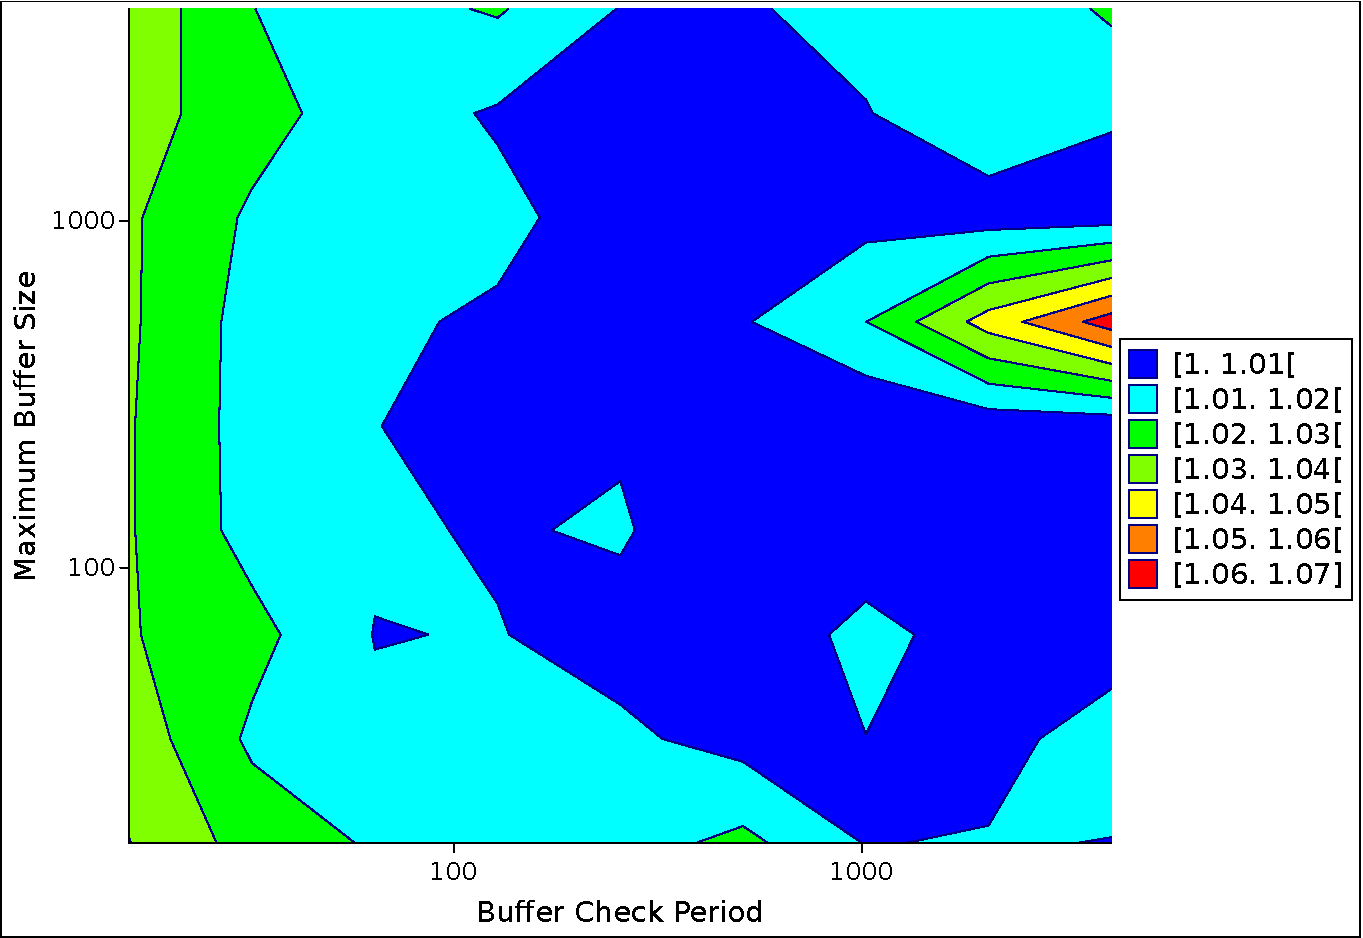
\includegraphics[width=6in]{chapters/parallel_mc/titan_comm_parameters.pdf}
  \end{center}
  \caption{\textbf{Neumann Ulam parallel algorithm history buffer
      check period vs. history buffer size sensitivity.} \textit{The
      color scale represents the ratio of the runtime of a particular
      parameter variation with the runtime from the faster parameter
      variation. A value of 1.02 on the color scale corresponds to a
      runtime 2\% longer than the faster time. All runtimes were
      within 6.5\% of the fastest observed case.}}
  \label{fig:titan_comm_parameters}
\end{figure}

Compared to the reference work, there was also not a significant
change in the runtime over the values of parameters tested with all
runtimes reported within 6.5\% of the fastest case observed. For this
work, a history buffer size of 4096 and a buffer check period of 128
performed best for the initial calculations. However, most values in
the range tested will give good performance. Brunner and Brantley
found that a value of 1024 was best for both parameters. For the
results observed here, these parameters were only 0.7\% slower than
the fastest case. It may be best practice to fix these parameters
internally at 1024 as both this work and the reference found these to
perform well several years apart on both different parallel machines
and for different transport sequences. Therefore, for the scaling
studies presented in the following sections, values of 1024 for both
the history buffer size and message check frequency will be used.

\clearpage

\subsection{Pure Domain Decomposition Scaling}
\label{subsec:pure_domain_decomp}

For the first set of scaling studies, we consider the parallel MCSA
algorithm where MSOD has not been used in the parallel Neumann-Ulam
algorithm. We refer to this case as pure domain decomposition where no
overlap or replication has been leveraged. Such a test will isolate
specifically the performance of Brunner and Brantley's algorithm as
applied to the Neumann-Ulam algorithm. For the strong scaling study,
the global diffusion problem size was fixed at \sn{1.6}{7} DOFs for
all solvers and the 16 core run used as the base case. MCSA was used
again with one stochastic history used per DOF in the Neumann-Ulam
solve to compute the correction for the acceleration with the
remainder of the problems and solver parameters the same as those for
the verification calculation given in
Table~\ref{tab:parallel_verification_parameters} and
Table~\ref{tab:parallel_mcsa_parameters}. As with all of the scaling
studies, 3 calculations for all data points were performed with the
average wall time reported and used for the efficiency
calculations. Figure~\ref{fig:titan_pure_strong_time} gives the wall
time per iteration for these calculations while
Figure~\ref{fig:titan_pure_strong} gives the results of the this study
with the given absolute efficiencies computed using
Eq~(\ref{eq:strong_scaling_absolute}). We report wall time per
iteration due to the fact that MCSA converged on the solution in 22
iterations while the Krylov solvers converged in 19 iterations.

\begin{figure}[t!]
  \begin{center}
    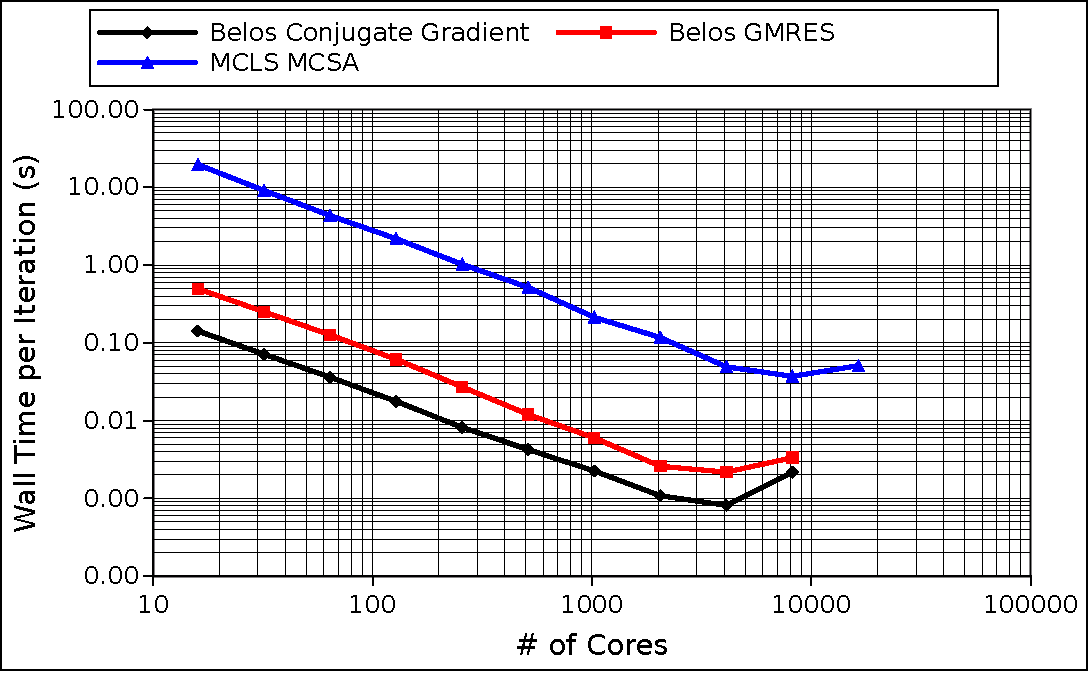
\includegraphics[width=6in]{chapters/parallel_mc/titan_pure_strong_time.pdf}
  \end{center}
  \caption{\textbf{Pure domain decomposition strong scaling wall time
      per iteration.} \textit{Wall time is reported per iteration
      because the methods converged in different numbers of
      iterations. MCLS is over an order of magnitude slower
      arithmetically than the Krylov solvers. GMRES executes more
      operations than conjugate gradient and is therefore slower as
      well.}}
  \label{fig:titan_pure_strong_time}
\end{figure}

\begin{figure}[t!]
  \begin{center}
    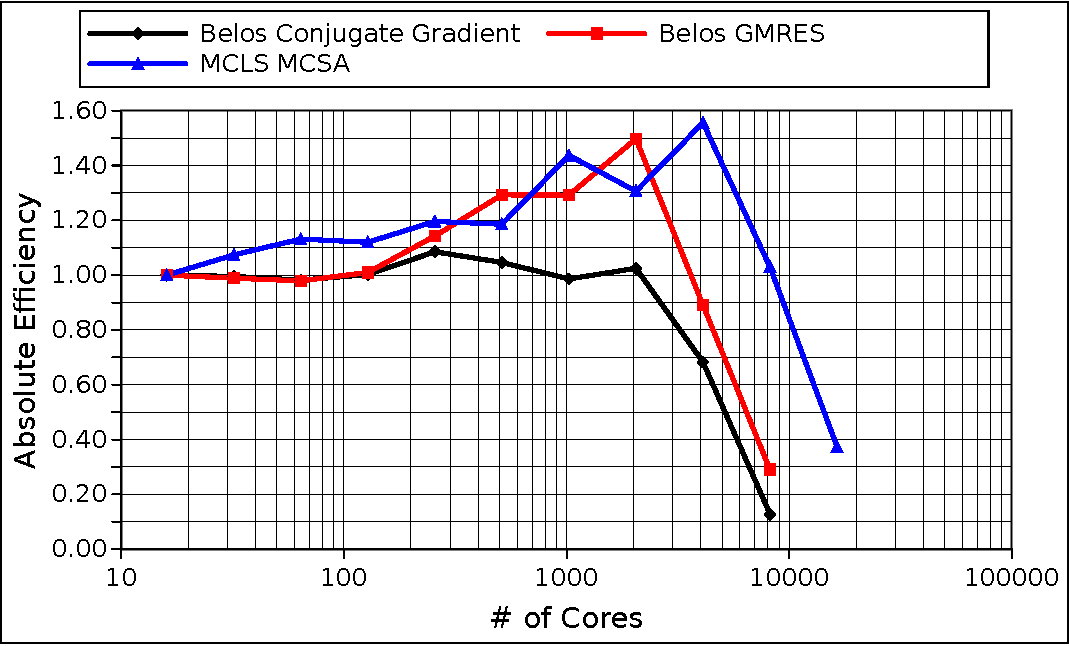
\includegraphics[width=6in]{chapters/parallel_mc/titan_pure_strong.pdf}
  \end{center}
  \caption{\textbf{Pure domain decomposition strong scaling absolute
      efficiency.}  \textit{Super-linear speed-up is from memory
      thrashing in the base case. MCLS is over an order of magnitude
      slower arithmetically, causing the higher efficiency. GMRES
      executes more operations than conjugate gradient, also creating
      a higher efficiency.}}
  \label{fig:titan_pure_strong}
\end{figure}

There are several key features of
Figure~\ref{fig:titan_pure_strong_time} and
Figure~\ref{fig:titan_pure_strong} worth noting. First, up to around
5,000 cores, all methods experience a super-linear improvement in
parallel efficiencies. For all methods, this increase is not a
function of the algorithmic efficiency as those computed using
Eq~(\ref{eq:algorithmic_efficiency}) remained at unity, meaning that
all computations converged in the same number of iterations relative
to the base case\footnote{When the algorithmic efficiency remains at
  unity for all calculations, the implementation efficiency is
  equivalent to the absolute efficiency and therefore is not presented
  here.}. Instead, what is happening here and was observed by Brunner
and Brantley in their work is that the large problem used to scale to
O(10,000) cores was large enough that memory thrashing was occurring
in the 16 core base case. As the number of cores in the strong scaling
study was increased and the local problem size decreased, more of the
local problem fit into the cache of the system, thus causing improved
serial performance and therefore enhanced runtimes. In this region of
super-linear efficiencies, we also observe larger efficiencies for
GMRES as compared to conjugate gradient. This occurs due to the fact
that conjugate gradient has a static set of operations performed at
every iteration while GMRES operates on a continually growing
subspace. In addition, the orthogonalization operations required to
generate that subspace consume much more time than the basic conjugate
gradient operations, causing a larger serial runtime and subsequently
higher efficiencies. For the same reasons, we also observe higher
efficiencies for the MCSA implementation due to the serial performance
of the implementation.

Beyond around 5,000 cores, the global problem size selected for this
strong scaling study causes the local problem size to shrink enough
that parallel communication costs begin to overtake arithmetic costs
on process. This takeover causes this effective strong scaling wall
that is observed in all methods. Using any more cores to solve this
particular global problem is not an efficient use of those parallel
resources. Furthermore, the fact that we see a very similar trends in
efficiencies for all methods means that they are bound by the same
parallel performance limitations in a strong scaling environment. This
is important as we can expect the same qualitative scaling performance
from MCSA if arithmetic optimization has been performed to improve the
serial performance of the implementation. In addition, these results
are valuable in that they show MCSA, when properly parallelized, has
the ability to be competitive on leadership-class computing platforms
with conventional subspace methods with good strong scaling observed
in the pure domain decomposition case to O(10,000) cores.

Next, we consider the weak scaling performance of the algorithm. In
this case, we fix the local problem size at \sn{4}{4} DOFs and
increase the number of processors used in the
simulation. Figure~\ref{fig:titan_pure_weak_time} gives the wall
time per iteration and Figure~\ref{fig:titan_weak_absolute} gives the
weak scaling absolute efficiencies for this problem as computed by
Eq~(\ref{eq:weak_scaling_absolute}). In general, the relative trends
when comparing MCSA to the Krylov methods are the same with MCSA and
GMRES scaling better than the conjugate gradient method due to the
increased amount of arithmetic work on-process. In addition, it is
important to note that the weak scaling of MCSA when properly
parallelized remains competitive with the Krylov methods keeping in
mind the artificial inflation of efficiencies.

\begin{figure}[t!]
  \begin{center}
    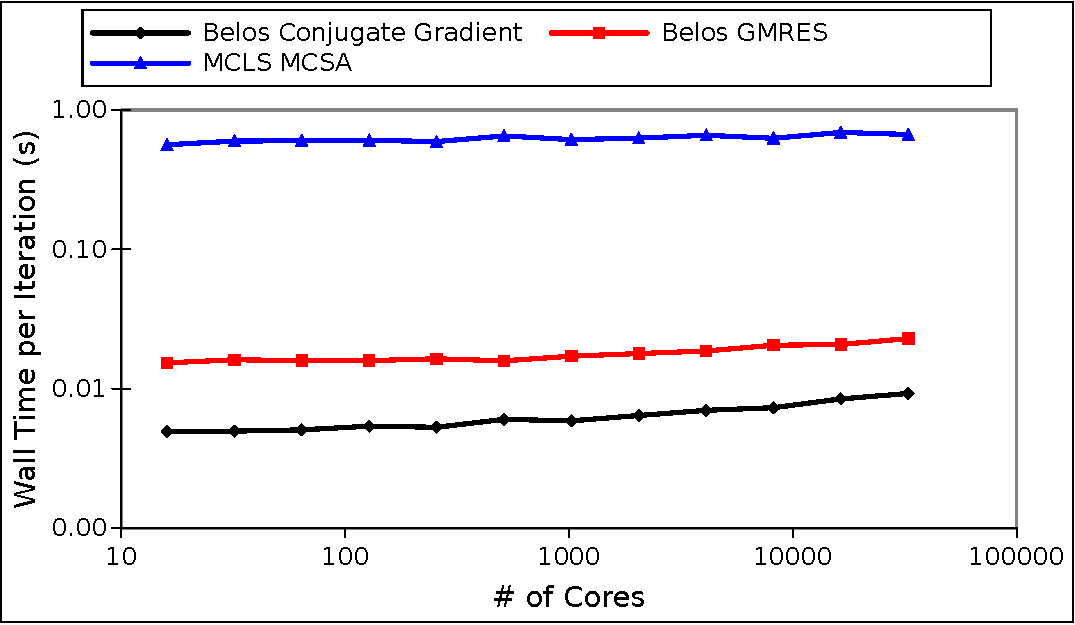
\includegraphics[width=6in]{chapters/parallel_mc/titan_pure_weak_time.pdf}
  \end{center}
  \caption{\textbf{Pure domain decomposition weak scaling wall time
      per iteration.} \textit{Wall time is reported per iteration
      because the methods converged in different numbers of
      iterations. MCLS is over an order of magnitude slower
      arithmetically than the Krylov solvers. GMRES executes more
      operations than conjugate gradient and is therefore slower as
      well.}}
  \label{fig:titan_pure_weak_time}
\end{figure}

\begin{figure}[t!]
  \begin{center}
    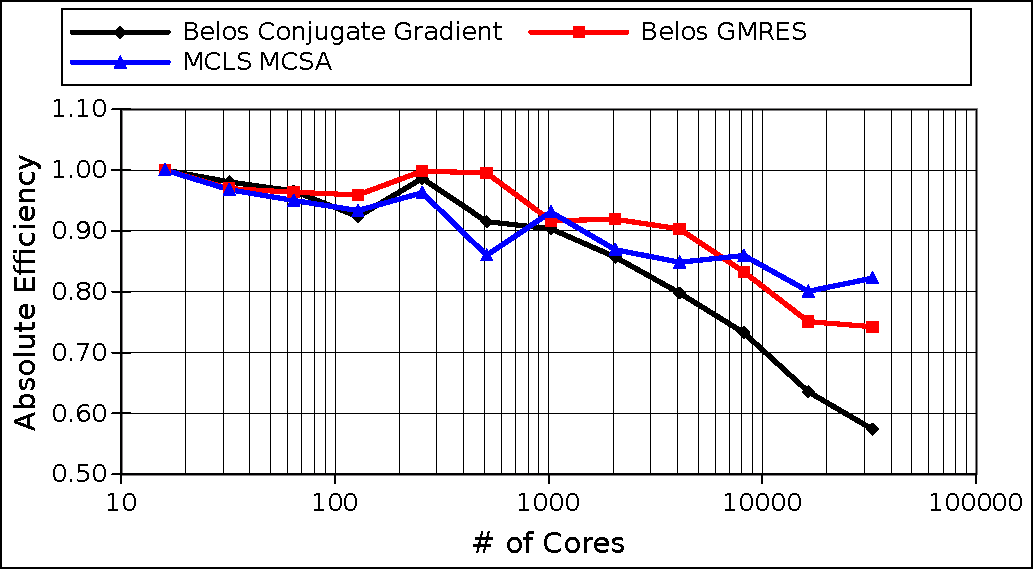
\includegraphics[width=6in]{chapters/parallel_mc/titan_weak_absolute.pdf}
  \end{center}
  \caption{\textbf{Pure domain decomposition weak scaling absolute
      efficiency.} \textit{MCLS is an over order of magnitude slower
      arithmetically, causing the higher efficiency. GMRES executes
      more operations than conjugate gradient, also creating a higher
      efficiency.}}
  \label{fig:titan_weak_absolute}
\end{figure}

As an additional means of comparison between MCSA and the Krylov
methods, we compute the algorithmic efficiencies of the calculations
using Eq~(\ref{eq:algorithmic_efficiency}). As shown in
Figure~\ref{fig:titan_weak_algorithmic}, the algorithm efficiency of
the Krylov algorithm improves as a function of the number of cores in
the problem due to the fact that the number of iterations required to
converge decreased from 20 in the base case to 19 and then to 18 for
the final set of weak scaling computations. When this reduction in
iterations is used to account for the observed runtimes and computed
absolute efficiencies for weak scaling we end up with the
implementation efficiencies computed using
Eq~(\ref{eq:implementation_efficiency}) given in
Figure~\ref{fig:titan_weak_implementation}. Because MCSA maintains the
same iterative performance as a function of global problem size in the
weak scaling study, the implementation efficiencies compare more
favorably to the Krylov methods. Using the implementation efficiency,
we are effectively measuring the parallel performance of a single
iteration for each method by looking at these implementation
efficiencies. As the global problem size increases, MCSA is less prone
to a drop in parallel efficiency. If optimization has been performed
and runtimes potentially approach those of the Krylov methods, this
comparison may not be as favorable. Overall, weak scaling performance
of the parallel MCSA algorithm is excellent for the pure domain
decomposition case with absolute parallel efficiencies of over 80\%
observed at over 32,000 cores.

\begin{figure}[t!]
  \begin{center}
    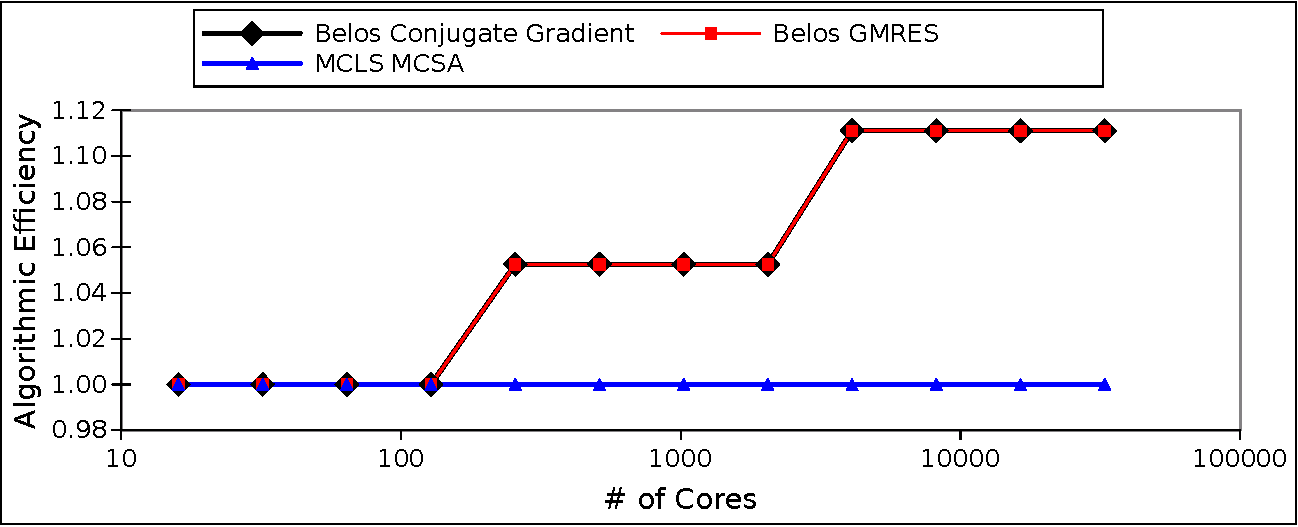
\includegraphics[width=6in]{chapters/parallel_mc/titan_weak_alg_eff.pdf}
  \end{center}
  \caption{\textbf{Pure domain decomposition weak scaling algorithmic
      efficiency.} \textit{As the global problem size was increased in
      the weak scaling study, both conjugate gradient and GMRES
      converged in fewer iterations, causing the rise in algorithmic
      efficiency.}}
  \label{fig:titan_weak_algorithmic}
\end{figure}

\begin{figure}[t!]
  \begin{center}
    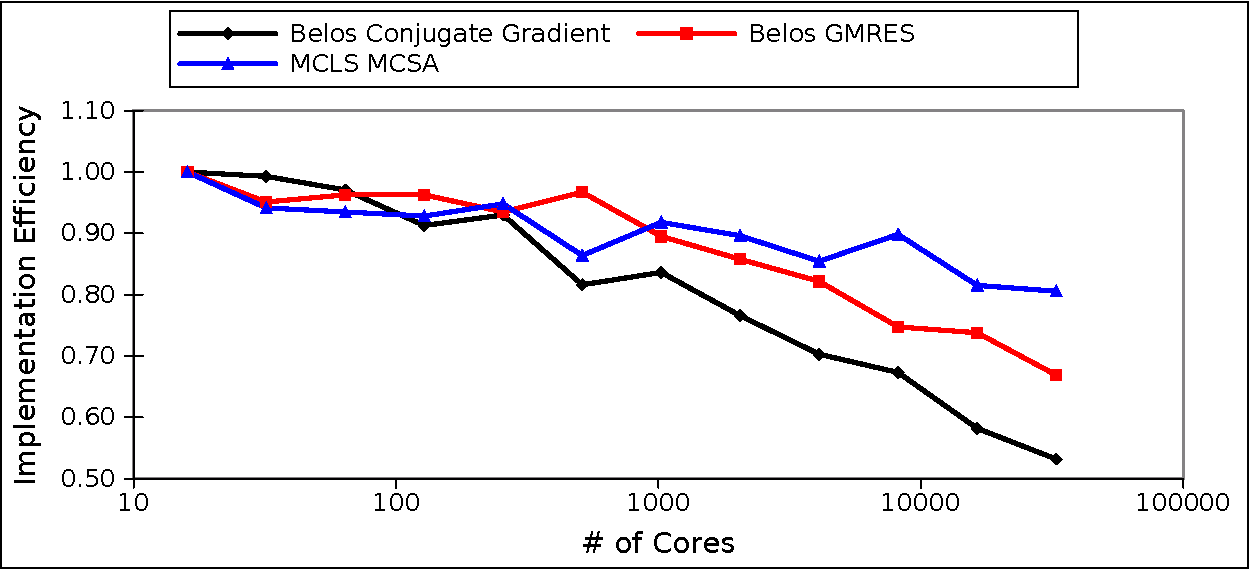
\includegraphics[width=6in]{chapters/parallel_mc/titan_weak_implementation.pdf}
  \end{center}
  \caption{\textbf{Pure domain decomposition weak scaling
      implementation efficiency.} \textit{Considering the scalability
      of a single iteration of the implementation, the inflated
      efficiencies of the MCLS MCSA implementation become more
      obvious. Implementation optimization will likely reduce the MCSA
      values to a level more comparable to the Belos values.}}
  \label{fig:titan_weak_implementation}
\end{figure}

In addition to comparing MCSA scaling to conventional methods, we also
motivate avoiding any type of master/slave algorithms at these high
levels of concurrency by comparing the binary communication tree
implementation used in the previous results with a parallel MCSA
implementation that uses the master/slave scheme to determine the end
of a history transport stage as shown in
Figure~\ref{fig:master_comm_tree}
instead. Figure~\ref{fig:titan_strong_bvsm} provides this comparison
using the strong scaling study while Figure~\ref{fig:titan_weak_bvsm}
gives the results of the comparison for the weak scaling study. In
both cases, the deficiencies caused by using the master/slave scheme
for transport completion are obvious. At around 1,000 cores, both the
strong and weak scaling performance seriously degrades while the
binary tree pattern maintains excellent performance. At this number of
cores, any extra work given to the master process, even if it amounts
to summing a handful of integers and checking for a few extra messages
as in this algorithm, grows enough to create serious load imbalance
and reduce performance.

\begin{figure}[t!]
  \begin{center}
    \includegraphics[width=6in]{chapters/parallel_mc/titan_strong_bvsm.pdf}
  \end{center}
  \caption{\textbf{Binary tree vs. master/slave communication scheme
      strong scaling absolute efficiency.} \textit{The master/slave
      scheme will not scale beyond $O(1,000)$ cores due to load
      imbalance.}}
  \label{fig:titan_strong_bvsm}
\end{figure}

\begin{figure}[t!]
  \begin{center}
    \includegraphics[width=6in]{chapters/parallel_mc/titan_weak_bvsm.pdf}
  \end{center}
  \caption{\textbf{Binary tree vs. master/slave communication scheme
      weak scaling absolute efficiency.}  \textit{The master/slave
      scheme will not scale beyond $O(1,000)$ cores due to load
      imbalance.}}
  \label{fig:titan_weak_bvsm}
\end{figure}

\clearpage

\subsection{Overlapping Domain Decomposition}
\label{subsec:overlapping_domain_decomp}

In the next set of scaling studies, we will explore how adding overlap
to the subdomains in the problem affects runtimes and parallel
performance as compared to the case with pure domain decomposition. To
do this, we utilize the set of analytic relations developed in
\S~\ref{sec:analytic_framework} to design these numerical
experiments. For the neutron diffusion problem used in these scaling
studies, the linear operator had a spectral radius of 0.787 and a
weight cutoff of \sn{1}{-2} was used with the Neumann-Ulam
solver. Using Eq~(\ref{eq:analytic_k}) gives an expected random walk
length of 19.22 transitions for any given history in the
problem. Using the mean-chord approximation given by
Eq~(\ref{eq:mean_chord_domain_leakage}), we then expect approximately
5.3\% of the histories born in a particular domain to leak out after
the first transport stage. By adding overlap, we aim to reduce this
fraction of communicated histories and therefore boost the parallel
performance of the algorithm. 

To determine the amount of overlap to test for the scaling studies, we
use a variation of Eq~(\ref{eq:step_k_length}) to determine how many
discrete states a history will move on average from its birth site. We
modify Eq~(\ref{eq:step_k_length}) to only account for discrete
movements:
\begin{equation}
  \sqrt{\bar{n^2_k}} = n_s \sqrt{k}\:,
  \label{eq:discrete_distance}
\end{equation}
where $\sqrt{\bar{n^2_k}}$ is now the root-mean-squared number of
discrete states a history will move from its birth site. For our
diffusion problem used in these scaling studies, we compute a value of
2.63 states per history for any of the dimensions of the system. This
means that we can expect to end up on average 2.63 states in both the
$i$ and $j$ dimensions away from the starting state. Therefore, we
will use the overlap generation algorithm outlined in
\S~\ref{subsec:msod_generation} such that we parametrically grow the
local domain using 1, 2, 3, and 5 levels to measure how scalability is
affected when this root-mean-squared number of states is
considered. For example, using 3 levels of overlap should keep over
50\% of the histories that would be communicated in the pure domain
decomposition case on-process as this is greater than the
root-mean-squared number of states we would expect a history to
travel.

For the performance metrics, we may use the same weak and strong
scaling efficiency metrics that we used for the pure domain
decomposition case. As we are comparing to the case without overlap
and are looking to boost performance relative to the case without
overlap, for both weak and strong scaling calculations we will use the
16-core case without overlap as the reference computation for all
efficiency measures reported. 

The absolute efficiency results from the strong scaling exercise are
given in Figure~\ref{fig:titan_strong_overlap}. Aside from the
boosting of efficiencies at 2,048 cores, little evidence of strong
scaling improvement is evident for all levels of overlap tested. To
further explore any potential benefits of adding overlap into the
system, Figure~\ref{fig:titan_strong_overlap_diff} gives the
difference in the efficiencies between all overlap cases and the
reference case without overlap at each core count. At smaller numbers
of cores, there is no observed benefit to using overlap to improve
strong scaling. The improvements noted at 2,048 cores are also present
here and account for the best efficiency improvements for all core
counts tested. at 16,384 cores, using 2 levels of overlap did give a
6.4\% boost in efficiency while at 1,024 cores this same amount of
overlap actually reduced the efficiency. Beyond 2 levels of overlap,
efficiency levels begin to fall with 5 levels of overlap performing
the worst for all cases. From this, we don't expect adding any more
overlap will improve the scalability of the algorithm and the best
strong scaling performance was observed when the number of overlap
levels is approximately equal to the root-mean-squared number of
states we expect a history to move from its starting point as computed
by Eq~(\ref{eq:discrete_distance}). We will defer an explanation of
the drop in efficiencies for levels of overlap beyond this value until
we have analyzed the weak scaling data.

\begin{figure}[t!]
  \begin{center}
    \includegraphics[width=6in]{chapters/parallel_mc/titan_strong_overlap.pdf}
  \end{center}
  \caption{\textbf{Strong scaling absolute efficiency with varying
      levels of overlap.} \textit{Values of 0, 1, 2, 3, and 5 levels
      of overlap were used as the problem had a root-mean-squared
      number of states of 2.63 for each history.}}
  \label{fig:titan_strong_overlap}
\end{figure}

\begin{figure}[t!]
  \begin{center}
    \includegraphics[width=6in]{chapters/parallel_mc/titan_strong_overlap_diff.pdf}
  \end{center}
  \caption{\textbf{Strong scaling absolute efficiency difference with
      respect to the 0 overlap base case.} \textit{Values of 1, 2, 3,
      and 5 levels of overlap are compared here with the absolute
      difference of the absolute efficiencies presented.}}
  \label{fig:titan_strong_overlap_diff}
\end{figure}

For weak scaling, the same study as in the pure domain decomposition
case was performed again with 1, 2, 3, and 5 levels of overlap. The
absolute parallel efficiencies from these calculations are given in
Figure~\ref{fig:titan_weak_overlap} and the differences in
efficiencies from the calculations without overlap. The results here
are much the same in that there is not a dramatic improvement in
scalability relative to the case without overlap. Opposite the strong
scaling calculation, overlap enhances weak scaling efficiencies at
lower core counts and degrades the efficiencies at higher core
counts. In addition, 1 level of overlap provided the best enhancement
of scalability when overlap was beneficial. 

\begin{figure}[t!]
  \begin{center}
    \includegraphics[width=6in]{chapters/parallel_mc/titan_weak_overlap.pdf}
  \end{center}
  \caption{\textbf{Weak scaling absolute efficiency with varying
      levels of overlap.} \textit{Values of 0, 1, 2, 3, and 5 levels
      of overlap were used as the problem had a root-mean-squared
      number of states of 2.63 for each history.}}
  \label{fig:titan_weak_overlap}
\end{figure}

\begin{figure}[t!]
  \begin{center}
    \includegraphics[width=6in]{chapters/parallel_mc/titan_weak_overlap_diff.pdf}
  \end{center}
  \caption{\textbf{Weak scaling absolute efficiency difference with
      respect to the 0 overlap base case.} \textit{Values of 1, 2, 3,
      and 5 levels of overlap are compared here with the absolute
      difference of the absolute efficiencies presented.}}
  \label{fig:titan_weak_overlap_diff}
\end{figure}

For both the strong and weak scaling studies, the parallel performance
of the algorithm was either marginally improved or not improved at
all. We would always expect an improvement in performance for using
overlap to prevent the transport of histories from domain to domain
during execution of the Neumann-Ulam algorithm. The reduction in
transport means a reduction in parallel communication and therefore
should never degrade the performance of the algorithm. It is true that
doing so in fact enhances Monte Carlo performance. However, the
Neumann-Ulam algorithm is not representative of the entire MCSA
algorithm. When overlap is used, an overlapping tally vector is
constructed in parallel such that multiple cores may own multiple
states in the system. When this occurs, the tally data associated with
these shared states must be communicated after the Neumann-Ulam solve
as outlined in \S~\ref{subsec:msod_algorithm}. This reduction
operation then builds the full MCSA correction vector in the
decomposition of the solution vector. 

Therefore, by building overlap we are in fact reducing parallel
communication during the Neumann-Ulam solve but we are simply
deferring that communication until after Monte Carlo transport when
the overlapping tally vector must be reduced. When overlap becomes
large enough (i.e. larger than the root-mean-squared number of
discrete states a history will travel), then the savings in
communication during the Neumann-Ulam solve start to become smaller
than the communication created in the overlapping tally vector
reduction. We see this in both the strong and weak scaling cases at
larger levels of overlap. For the strong scaling case, we see better
performance improvement at higher core counts because the total number
of overlapping states on each core is smaller from the local problem
size shrinking. For weak scaling, we see better performance
improvement at lower numbers of cores because although the local
overlap size is fixed, the global amount of overlap is growing with
core count and therefore reducing the performance of the tally
reduction operation. 

Based on this data, a few levels of overlap within the expected
distance of travel for a history may offer some marginal improvement
in scalability, however, it is not as effective as one might think
given its improvement to reactor physics calculations as observed in
the literature. This is largely due to the density of states in the
system that creates the described performance bottlenecks in the
overlapping tally vector reduction operation. In a Monte Carlo
particle simulation, these overlapping tally reduction operations are
not expected to be performed at the speed they are required in
MCSA. For example, in a criticality calculation with overlapping
domains, we would expect to perform as many parallel tally vector
reduction in a particle transport simulation as there are particle
stages required for convergence of the eigenvalue. However, these
particle stages will likely be much more costly in terms of wall time
relative to a Neumann-Ulam solve in an MCSA iteration due to the more
extensive particle physics and logic structure that must be
evaluated. Therefore, we can expect this overlapping tally reduction
to be less significant to scalability in those operations. We do not
have as complicated a logic structure in a history random walk for the
Neumann-Ulam method and therefore overlap can inhibit scalability if
too large.

\clearpage

\subsection{Multiple Set Domain Decomposition}
\label{subsec:ms_decomposition}

We next look to apply replication to the problem in the form of
multiple sets. As the previous analysis showed overlap to be of little
assistance in improving scalability, we only apply multiple sets to
the problem with pure domain decomposition within the sets for these
scaling studies. Before performing parallel scaling studies using
multiple sets, several aspects of the replicated parallel problem must
be considered in order to effectively craft the studies and interpret
their results. First is the question of how many stochastic histories
to use to generate the correction vector in the MCSA iteration. For
this work we consider two choices; the split case and the fully
replicated case. As an example of these cases, consider a single set
problem where 20,000 histories are used in the Monte Carlo solve. If
we choose the split case, then solving the same problem with 2 sets
would give 10,000 histories in each set and 4 sets would give 5,000
histories in each set. Splitting the histories in this way provides
the same global number of histories used to compute the correction in
the single set problem. We expect to reduce the time to solution by
doing this as each individual set solve will occur faster in an almost
linear fashion with the reduced number of histories. For the
replicated history case, each additional set in the problem will use
just as many histories as the single set case. Using 2 sets with fully
replicated histories for our example problem then has each set
computing 20,000 histories with 40,000 global histories in the
computation. For the 4 set case, the number of global histories is
increased to 80,000. We also expect this type of replication to reduce
the time to solution as the extra global histories should reduce the
stochastic uncertainty in the correction vector and reduce the overall
number of MCSA iterations required to converge.

\subsubsection{Strong Scaling with Multiple Sets}
\label{subsubsec:ms_strong}

For the strong scaling study, we apply the additional sets as
follows. Using the same problems as the pure domain decomposition
scaling study, the multiple sets are used to replicate those problems
and boost the core count. For example, for the 4 set case, the data
point at 64 cores has the same $N/P$ ratio in one set as the single
set problem with 16 cores. This is due to the fact that $N$ is fixed
for the strong scaling study and 4 replications gives a set size of 16
cores. For the 2 set case, the 32 core data point is solving the same
$N/P$ problem in a set as the 16 core base case.

In addition to considering the replicated domain, we must also
consider how to modify the efficiencies we will compute. For the
strong scaling case, recall that the objective is to decrease the time
to solution for a given global problem size $N$ by increasing
$P$. Therefore, we may use Eqs~(\ref{eq:strong_scaling_absolute_ref}),
(\ref{eq:algorithmic_efficiency}), and
(\ref{eq:implementation_efficiency}) to compute the various strong
scaling efficiencies, but we must modify the reference computation in
each of these formulas to reflect our objective. For all efficiency
computations, the 16 core single set computation will be used as the
reference case. By adding more cores to the problem, either by
replicating with multiple sets, or decreasing the local problem size,
any computational resources added to the problem should aim to result
in speedup of this reference case. If this speedup for one technique
of adding cores is less than another, then that technique is deemed a
less efficient use of those computational resources.

For the multiple sets problem, the single set strong scaling study
from the pure domain decomposition base case was repeated for multiple
sets with both splitting of histories across sets and full replication
of histories across sets using both 2 and 4
sets. Figure~\ref{fig:titan_strong_ms_time} gives the actual wall
times for these computations. There are two important features to note
in the wall time data. First, splitting the histories among sets
instead of replicating them is faster due to the fact that cutting the
number of histories in half reduces the time of an iteration by a
factor that is nearly linear while increasing linearly the number of
histories through replication does not decrease the iterations
required to converge by a linear factor. Second, until the strong
scaling wall is hit starting at around 10,000 cores, the single set
case actually performs the fastest with only marginal improvement in
runtimes at higher numbers of cores with more sets. At these larger
numbers of cores, however, the improvements are so modest that one is
better off running the same problem using a single set at lower core
counts to conserve computational resources while maintaining a good
time to solution.

\begin{figure}[t!]
  \begin{center}
    \includegraphics[width=6in]{chapters/parallel_mc/titan_strong_ms_time.pdf}
  \end{center}
  \caption{\textbf{Wall time in seconds to solution for each case for
      the strong scaling study with multiple sets.} \textit{Until the
      strong scaling wall is reached at O(10,000) cores, the single
      set case performs the best. For the multiple set cases, it is
      faster to split histories among sets and maintain iterative
      performance rather than replicate histories to improve iterative
      performance.}}
  \label{fig:titan_strong_ms_time}
\end{figure}

From this timing data we then compute the absolute efficiencies for
strong scaling as given in Figure~\ref{fig:titan_strong_ms_eff} using
the 16-core single set calculation as the reference case. As observed
in the timing data, because the single set case had the fastest run
times up to the strong scaling wall it also has the best observed
efficiencies. For the 2 set case with history splitting, although the
time to perform an iteration was nearly cut in half, the extra
parallel overhead associated with reducing the tally across the blocks
to combine the set results increases run times and reduces
efficiencies. This reduction across blocks is even more obvious for
the 4 set case. For the replicated cases, we do observe a flat region
of parallel efficiencies at larger core counts (up to around 32,000
for the 4 set case with history replication) showing improved scaling
within context of not considering the single set
calculation. Unfortunately, the additional cores do not reduce the
runtime of the global problem as efficiently as expected. Ultimately,
all cases effectively hit the strong scaling wall at the same time at
around O(10,000) cores.

We expect this if we consider the fact that adding sets to the problem
is in itself effectively a form of strong scaling. For any given
problem of fixed size $N$, adding extra sets to the computation
decreases the global ratio of $N/P$ as $P$ will grow with the addition
of sets (although $N/P$ is constant within a set). For the split
history case, the splitting further exacerbates this situation by
further decreasing the amount of histories that will be computed in
the local domain, giving a larger ratio of communication to work in
the Monte Carlo solve. As with with single set results, we also
observe some efficiencies greater than unity for the multiple set
cases also due to improved cache utilization. 

Although not as dramatic as one might originally expect from
introducing replication, there are some modest gains in efficiencies
at high core counts by using multiple sets. Of interest here is where
the multiple set cases perform better than the single set case after
the single set case has hit the strong scaling wall. In
Figure~\ref{fig:titan_strong_ms_eff}, at 16,384 cores the single set
case operates at 38\% efficiency while at the same number of cores,
the 2 set case with history replication operates at 58\%
efficiency. This is reasonable improvement in the use of those
computational resources, gained by replicating the problem. Beyond
16,384 cores, there is not a compelling reason to use more
computational resources for the this problem.

\begin{figure}[t!]
  \begin{center}
    \includegraphics[width=6in]{chapters/parallel_mc/titan_strong_ms_eff.pdf}
  \end{center}
  \caption{\textbf{Multiple set absolute parallel efficiency.}
    \textit{Computed relative to the 16-core 1-set base case. Using a
      single set is the best means by which to improve strong scaling
      up to the strong scaling wall. At higher core counts past where
      the single set case hits the strong scaling wall adding sets can
      provide some improvements in efficiencies.}}
  \label{fig:titan_strong_ms_eff}
\end{figure}

Also of interest here is the effect of splitting histories among sets
versus replicating them on the iterative performance of the
method. Table~\ref{tab:ms_strong_alg_eff} gives the iterations
required to converge and computed algorithmic efficiencies for each of
the cases presented in the strong scaling data. As expected, splitting
histories maintains a fixed global number of histories and therefore
maintained the number of iterations required to converge relative to
the single set base case. When histories were replicated, adding sets
decreased the number of iterations required to converge in a nonlinear
fashion. Therefore, increasing the number of histories per MCSA
iteration improves algorithmic efficiency. Using these algorithmic
efficiencies, the implementation efficiencies for the multiple set
cases were computed and are given in
Figure~\ref{fig:titan_strong_ms_impeff}. From these results, we see
that the replicated history cases are even less efficient than in the
absolute case with respect to the performance of a single
iteration. Not only do we have the additional parallel overhead of
doing the block level reduction, but we also have additional histories
that increase the time to solution for a single iteration.

\begin{table}[h!]
  \begin{center}
    \begin{tabular}{lcc}\hline\hline
      \multicolumn{1}{l}{Case}& 
      \multicolumn{1}{c}{Iterations}&
      \multicolumn{1}{c}{$\eta_{alg}$} \\\hline
      1 & 22 & 1.0 \\
      2-split & 22 & 1.0 \\
      2-replicated & 16 & 1.375 \\
      4-split & 22 & 1.0 \\
      4-replicated & 13 & 1.692 \\
      %%
      \hline\hline
    \end{tabular}
  \end{center}
  \caption{\textbf{Strong scaling algorithmic efficiency using
      multiple sets.} \textit{Replicating histories improves
      algorithmic efficiency by converging in fewer iterations.}}
  \label{tab:ms_strong_alg_eff}
\end{table}

\begin{figure}[t!]
  \begin{center}
    \includegraphics[width=6in]{chapters/parallel_mc/titan_strong_ms_impeff.pdf}
  \end{center}
  \caption{\textbf{Multiple set strong scaling implementation
      efficiency.} \textit{Computed relative to the 16-core 1-set base
      case. Considering iterations required to converge, the
      performance of the split history cases at much better than the
      cases with history replication.}}
  \label{fig:titan_strong_ms_impeff}
\end{figure}

\clearpage

\subsubsection{Weak Scaling with Multiple Sets}
\label{subsubsec:ms_weak}

Next, we continue to a weak scaling study of the multiple sets
problem. In the same way as the strong scaling study, we will modify
the pure domain decomposition study to account for the additional
replication. For each calculation in the single set study, that
problem will be replicated either 2 or 4 times with both split and
replicated histories to assess the effects on scalability and
runtime. Figure~\ref{fig:titan_weak_ms_time} gives the wall times from
the multiple sets weak scaling study. Of primary importance here is
the fact that adding sets to the problem with both split and
replicated histories actually decreases the time to solution. This was
not observed in the strong scaling case until much larger core counts
as the multiple set computations hit the strong scaling wall after the
single set computation.

This result is significant in that it shows a solution technique in
which the linear problem can actually be replicated and enhance time
to solution, something that cannot be achieved with conventional
methods. At larger core counts, however, this reduction in compute
time is not as large as at lower core counts due to the fact that the
tally reduction across blocks requires more resources and those
resources are clearly growing with core count (most obviously in the 4
set case with split histories). In addition, at 131,072 cores for the
largest 4 set computation, load balance is likely becoming an issue
due to the linear system and subsequent parallel matrix and vector
operations only occurring on a subset of the entire processor space of
the problem while the Monte Carlo calculation is occurring on all
processors.

\begin{figure}[t!]
  \begin{center}
    \includegraphics[width=6in]{chapters/parallel_mc/titan_weak_ms_time.pdf}
  \end{center}
  \caption{\textbf{Wall time in seconds to solution for each case for
      the weak scaling study with multiple sets.}}
  \label{fig:titan_weak_ms_time}
\end{figure}

For a multiple set analysis of the weak scaling timing results, we
again have to consider that adding sets to the problem is actually a
form of strong scaling. Consider a single set problem ($S=1$) for a
given $P$ and $N$. When that problem is now solved using 2 sets we
have $S=2$, $N$ and $2P$. For any number of sets we then have a global
problem size of $N$ while the number of processors is $SP$ where $P$
is the number of processors in the single set case. Therefore, $N/P$
is no longer fixed in the weak scaling study but rather $N/(SP)$ is
fixed. As a result, we modify the weak scaling absolute efficiency
relationship to account for this fact:
\begin{equation}
\eta_{weak}(M|N,P|Q,S) = \frac{T(M,Q)}{S \times T(N,P)}\:,
  \label{eq:ms_weak_efficiency}
\end{equation}
where now the absolute efficiency is a function of the number of sets
in the problem and again $M/Q = N/P$. As with the strong scaling
study, we will use the 16-core single set case as the reference
computation for efficiencies. Interestingly,
Eq~(\ref{eq:ms_weak_efficiency}) has a very similar form to the strong
scaling efficiency given by Eq~(\ref{eq:strong_scaling_absolute}),
representative of the strong scaling nature of adding additional
sets. For problems where adding sets improves time to solution, this
new weak scaling formulation accounts for how efficiently those extra
resources are incorporated into the problem. Without such a
modification, the largest case run for the split 4 set case would have
a computed weak scaling efficiency of nearly 100\% using the standard
formula for absolute efficiency. However, using 4 times as many cores
as the single set case increased the runtime for a fixed global
problem size and therefore we would actually expect to compute a very
low efficiency that shows this very poor use of resources.

Figure~\ref{fig:titan_weak_ms_eff} gives the results of the weak
scaling efficiency computations using the multiple set metric given by
Eq~(\ref{eq:ms_weak_efficiency}). Although we do reduce the time to
solution over the base cases for nearly all data points, the
observation here is that the reduction in time to solution is still
not large enough to efficiently use all resources. For example, for
the 2 set case to be a perfect use of resources with either split or
replicated histories, the runtime of that calculation must be half of
that for the single set case. For the 4 set case, this run time should
be a quarter of the single set case for perfect scaling. This was not
the observation for the runtimes in
Figure~\ref{fig:titan_weak_ms_time} and therefore the single set case
is still the most efficient use of computational resources in this
scaling study.

\begin{figure}[t!]
  \begin{center}
    \includegraphics[width=6in]{chapters/parallel_mc/titan_weak_ms_eff.pdf}
  \end{center}
  \caption{\textbf{Weak scaling absolute efficiency relative to
      16-core 1-set base case.}}
  \label{fig:titan_weak_ms_eff}
\end{figure}

As in the strong scaling case, splitting and replicating histories
across sets had effectively the same results for the weak scaling
study with the iterations to converge and computed algorithmic
efficiencies given by Table~\ref{tab:ms_weak_alg_eff}. Again, when the
implementation efficiencies are computed, we see in
Figure~\ref{fig:titan_weak_ms_impeff} that splitting histories among
sets is still a more efficient manner of introducing multiple sets
rather than replicating histories in an attempt to reduce the number
of iterations required to converge.  Here we also note that this is
not a true weak scaling study as indicated by
Eq~(\ref{eq:ms_weak_efficiency}) but rather an odd combination of both
weak and strong scaling. Regardless of this, although multiple sets
are not the most efficient use of resources in this analysis, they do
enhance the time to solution through replication and do so
significantly at core counts of O(1,000) and lower. In both the weak
and strong scaling cases, due to the additional computational and
communication overhead of adding sets to the system, one should never
expect to seriously boost parallel efficiencies for MCSA using this
technique except for certain instances past the strong scaling wall in
a purely strong scaling environment. In a weak scaling environment,
although no efficiency increase will be noted, one can expect an
enhancement of time to convergence by replicating.

\begin{table}[h!]
  \begin{center}
    \begin{tabular}{lcc}\hline\hline
      \multicolumn{1}{l}{Case}& 
      \multicolumn{1}{c}{Iterations}&
      \multicolumn{1}{c}{$\eta_{alg}$} \\\hline
      1 & 22 & 1.0 \\
      2-split & 22 & 1.0 \\
      2-replicated & 16 & 1.375 \\
      4-split & 22 & 1.0 \\
      4-replicated & 13 & 1.692 \\
      %%
      \hline\hline
    \end{tabular}
  \end{center}
  \caption{\textbf{Weak scaling algorithmic efficiency using multiple
      sets.} \textit{Replicating histories improves algorithmic
      efficiency by converging in fewer iterations.}}
  \label{tab:ms_weak_alg_eff}
\end{table}

\begin{figure}[t!]
  \begin{center}
    \includegraphics[width=6in]{chapters/parallel_mc/titan_weak_ms_impeff.pdf}
  \end{center}
  \caption{\textbf{Implementation parallel efficiency relative to 16-core
      1-set base case.}}
  \label{fig:titan_weak_ms_impeff}
\end{figure}

\clearpage

\subsection{Subdomain Neumann-Ulam}
\label{subsec:full_clip}

Based on the analysis of the pure domain decomposed MCSA algorithm and
subsequently the multiple sets and overlapping domain implementation,
one may ask then ask if there is any need to communicate histories
from domain-to-domain at all. Overlap was not as successful because
because the additional communication required to reduce the
overlapping tally vector eventually becomes larger than the
communication savings during Monte Carlo transport. In addition, for
local domains that are large enough to get good performance
(e.g. those used in the weak scaling studies), then our analytic
relationships for domain leakage, and in particular
Eq~(\ref{eq:mean_chord_domain_leakage}), tell us that only about 5\%
of the histories in this diffusion problem will leave the domain in
the first place.  If that is true, then perhaps without any overlap or
communication, just doing local Monte Carlo transport such that
histories are terminated upon reaching the domain boundary may be
satisfactory for accelerating the MCSA iteration. In this case,
histories near the boundaries of the domain may be truncated before
reaching the weight cutoff if they reach the domain boundary
first. This truncation has the potential to increase the stochastic
uncertainty of the Neumann-Ulam result and therefore increase the
number of MCSA iterations required to converge. In addition, the
scalability of the method will then be purely limited by the parallel
matrix and vector operations required to implement the remainder of
the algorithm on the subset of processors containing the linear
problem.

Considering using MCSA in this way such that the Monte Carlo solve
occurs only in the subdomains casts the method as more of a true
domain decomposition as outlined by Chapter 14 of Saad's text on
iterative methods \citep{saad_iterative_2003}. Compared to traditional
domain decomposition methods we see many similarities including the
potential to overlap the subdomains to improve the results. By
building the boundary data as outlined in
\S~\ref{subsec:domain_generation}, we are effectively gathering one
level of the adjacent domains, albeit in this case to satisfy the data
requirements of the Monte Carlo estimators. Furthermore, the fact that
we are using residual Monte Carlo to compute the correction vector
casts MCSA as a stochastic realization of an additive Schwarz method
with a fixed point iteration used as a relaxation step\footnote{See
  section 14.3.3 in \citep{saad_iterative_2003} for a full definition
  of the additive Schwarz method.}. Both the fixed point iteration and
the computation of the residual propagate the solution from individual
subdomains to the others through the matrix-vector multiply operation
after all subdomain Monte Carlo solves have been completed. Perhaps an
even more important consequence of viewing MCSA as a stochastic
additive Schwarz procedure is that it has the potential to more
readily fit as an accelerator into other linear solver techniques
including GMRES or potentially as a preconditioner.

Using the Neumann-Ulam solver to compute the MCSA correction only in
the subdomains, the strong and weak scaling studies were repeated to
assess the performance gains made by eliminating communication in the
Monte Carlo solver. For each scaling study, the 16-core base case with
Monte Carlo communication was used as the reference point for
efficiency computations in order to measure how eliminating
communication boosts
efficiencies. Figure~\ref{fig:titan_strong_subdomain} gives the
results of the strong scaling study and
Figure~\ref{fig:titan_weak_subdomain} gives the results of the the
weak scaling study in terms of absolute efficiencies. In both cases,
the benefits to parallel performance of using MCSA as a subdomain
solver are obvious. In the strong scaling case we make the important
observation that we hit the strong scaling wall at the same time with
and without the additional Monte Carlo communication. Although the
Monte Carlo communication did contribute to the efficiency decrease,
it is clear that the remaining matrix and vector operations are the
primary impediment to scalability. Furthermore, we see an even greater
rise above unity in efficiencies because there is less communication
overhead hiding the better cache utilization as the local problem size
shrinks. At 16,384 cores, performing the subdomain solves boost the
absolute efficiency from 38\% to 67\% relative to the reference case.

In the weak scaling study, we do not have the scaling wall to contend
with and eliminating Monte Carlo communication through subdomain
solves provides an effectively linear boost in the weak scaling
absolute efficiency. We still see a small reduction in weak scaling
efficiency as a function of core count due to the communication
overhead for the parallel matrix and vector operations. Here we
observe super unitary efficiencies for the subdomain case as there was
a substantial improvement in runtimes relative to the 16-core base
case with Monte Carlo communication.

\begin{figure}[t!]
  \begin{center}
    \includegraphics[width=6in]{chapters/parallel_mc/titan_strong_subdomain.pdf}
  \end{center}
  \caption{\textbf{Strong scaling absolute efficiency for pure domain
      decomposition.} \textit{The subdomain Monte Carlo solver
      improves the parallel efficiency and therefore time to solution
      by eliminating all parallel communication during the Monte Carlo
      solve.}}
  \label{fig:titan_strong_subdomain}
\end{figure}

\begin{figure}[t!]
  \begin{center}
    \includegraphics[width=6in]{chapters/parallel_mc/titan_weak_subdomain.pdf}
  \end{center}
  \caption{\textbf{Weak scaling absolute efficiency for pure domain
      decomposition.} \textit{The subdomain Monte Carlo solver
      improves the parallel efficiency and therefore time to solution
      by eliminating all parallel communication during the Monte Carlo
      solve.}}
  \label{fig:titan_weak_subdomain}
\end{figure}

Of additional concern for the subdomain method is the potential
decrease in iterative performance due to the fact that histories near
the boundary will potentially have their random walk truncated, thus
decreasing the information available to compute the correction
vector. For both the weak and strong scaling study, all calculations
with split histories converged in 22 or in only a few cases 21
iterations for both the subdomain solve and the solve with
communication giving an algorithmic efficiency of 1.048 for all
cases. This small improvement in iteration count was not observed to
be a function of problem size, number of processors, or whether the
subdomain method was used. For the replicated history cases, the
algorithmic efficiency improvement was not as good as when
communication was allowed for the Monte Carlo algorithm. For these
calculations, the number of iterations to converge was reduced to 18
or 19 in both the strong and weak scaling studies with lower core
counts converging in fewer iterations.

Therefore, there is no reason to expect overlap to improve the
iterative or scaling performance of the method as iterative
performance is maintained without it for this particular
problem. Overlap is not as effective because histories relinquish most
of their useful information within the first few steps (which is why
we can use such a large weight cutoff and there is an insensitivity to
weight cutoff as shown in
Figure~\ref{fig:estimator_wc_iters}). Keeping them around longer with
overlap to do extra work in the local domain will not improve
iterative performance and thus increase compute times.

As a final analysis of MCSA using subdomain Monte Carlo, the multiple
sets scaling studies are repeated to determine if any performance
benefits are made from replication by eliminating Monte Carlo
communication. Figure~\ref{fig:titan_strong_subdomain_ms_time} gives
the runtimes for the strong scaling calculation and
Figure~\ref{fig:titan_strong_subdomain_ms} the computed absolute
efficiencies. For the weak scaling studies,
Figure~\ref{fig:titan_weak_subdomain_ms_time} gives the wall times and
Figure~\ref{fig:titan_weak_subdomain_ms} the efficiencies. For both
scaling studies, the results are effectively the same as for the case
with Monte Carlo communication. This is again due to the fact that
adding sets to the problem is not only an exercise in strong scaling
but it also adds additional parallel overhead in the form of the tally
vector reduction across blocks.

From a parallel performance perspective, MCSA may then be best used in
a mode where the Monte Carlo is performed over only the subdomains
with no replication or overlap added to the system. In this mode,
iterative performance is maintained relative to the solutions with
communication even for more ill-conditioned problems with larger
spectral radii. Furthermore, no overlap was required to maintain
iterative performance be letting histories near the boundary take a
few more steps in their random walks. If in the future there are
ill-conditioned problems where using subdomain Monte Carlo reduces the
algorithmic efficiency of MCSA due to the information lost in the
correction vector, overlap would be a viable mechanism to potentially
maintain that iterative performance, keeping in mind the potential
impacts on scalability that were observed in this work. However,
although eliminating all Monte Carlo communication was observed to be
the best mode of use for MCSA, the parallel Monte Carlo methods
developed for this work still provide value for cases where only a
Monte Carlo solution is desired. In those cases, full transport of the
Monte Carlo histories are required in order to generate the correct
solution.

\begin{figure}[t!]
  \begin{center}
    \includegraphics[width=6in]{chapters/parallel_mc/titan_strong_subdomain_ms_time.pdf}
  \end{center}
  \caption{\textbf{Strong scaling total wall time with multiple sets
      and subdomain Monte Carlo.} \textit{Adding multiple sets has in
      general a negative effect on the wall time as was observed for
      the case with full Monte Carlo transport.}}
  \label{fig:titan_strong_subdomain_ms_time}
\end{figure}

\begin{figure}[t!]
  \begin{center}
    \includegraphics[width=6in]{chapters/parallel_mc/titan_strong_subdomain_ms.pdf}
  \end{center}
  \caption{\textbf{Strong scaling absolute efficiency for with
      multiple sets and subdomain Monte Carlo.} \textit{Increased wall
      times from adding parallel reduction operations for multiple
      sets reduces parallel scalability at lower core counts but gives
      a higher efficiency at the strong scaling wall.}}
  \label{fig:titan_strong_subdomain_ms}
\end{figure}

\begin{figure}[t!]
  \begin{center}
    \includegraphics[width=6in]{chapters/parallel_mc/titan_weak_subdomain_ms_time.pdf}
  \end{center}
  \caption{\textbf{Weak scaling total wall time with multiple sets and
      subdomain Monte Carlo.} \textit{The addition of the set tally
      reduction is significant with cost of the reduction observed as
      core count grows.}}
  \label{fig:titan_weak_subdomain_ms_time}
\end{figure}

\begin{figure}[t!]
  \begin{center}
    \includegraphics[width=6in]{chapters/parallel_mc/titan_weak_subdomain_ms.pdf}
  \end{center}
  \caption{\textbf{Weak scaling absolute efficiency for with multiple
      sets and subdomain Monte Carlo.} \textit{Weak scaling
      efficiencies are not improved at large core counts when multiple
      sets are added.}}
  \label{fig:titan_weak_subdomain_ms}
\end{figure}

\chapter{Conclusion\ }
\label{ch:conclusion}

For high fidelity simulations of nuclear reactors, physics solutions
are required with speed and accuracy. When the problems become large
enough, such as the simulation of an entire reactor core,
leadership-class computing facilities must be leveraged on the grounds
of requirements for both time to solution and the amount of memory
required to contain the description of the entire problem. Looking
forward to the next generation of machines, concurrency will go up and
available memory will go down, putting pressure on physics application
developers to research and develop solution techniques that can
efficiently leverage this hardware. In nuclear reactor simulation,
both neutron transport and fluid flow calculations consume a vast
amount of computational time in order to properly characterize both
steady state operational characteristics and transient accident
scenarios. In both cases, we desire solution techniques that are aware
of coming changes in hardware.

In this work, we have presented Monte Carlo Synthetic Acceleration as
a viable solution technique for both neutron transport and fluid flow
problems on future hardware. To do this, we carried out three research
and development activities. First, we applied MCSA to the $SP_N$ form
of the neutron transport equation and analyzed the preconditioning
requirements and subsequent performance of the method when compared to
conventional practices. Second, we used the knowledge gained from the
research on neutron transport to develop the FANM method for nonlinear
problems and studied its performance on three different benchmarks for
the Navier-Stokes equations to demonstrate its applicability. Finally,
we parallelized MCSA such that it may be applied to physics problems
on leadership-class computing platforms.

In this chapter, we review the work presented in this document and
describe how this work met the goals of the research. We then
reiterate the important issues discovered during the course of this
work and develop a strategy for future work to potentially alleviate
them. Finally, we close with some final remarks regarding Monte Carlo
Synthetic Acceleration.

%%---------------------------------------------------------------------------%%
\section{Monte Carlo Synthetic Acceleration Methods for the $SP_N$ Equations\ }
\label{sec:spn_conclusion}
This work demonstrates the first application of MCSA to the neutron
transport problem. To do this, we used the $SP_N$ form of the
Boltzmann transport equation. In this form, the transport equation
takes on a diffusion-like form where the angular character of the flux
is accounted for in moment terms much like those found in the $P_N$
equations. To meet the goals of this work and drive the research and
development of MCSA for application to light water reactor problems, a
difficult nuclear fuel assembly criticality calculation was used in a
set of numerical experiments. These calculations were enabled by
incorporating MCSA as a solution scheme into the k-eigenvalue solver
in the Exnihilo production neutronics code base at Oak Ridge National
Laboratory.

When applying the new technique to the fuel assembly problem, it was
initially found that MCSA could not converge the problem with basic
Jacobi-based preconditioning. This was discovered to be due to the
fact that the transport operator generated in the eigenvalue
calculation was very ill-conditioned as a result of the large amount
of neutron scattering in the light water moderator. The more
scattering present in the system, the longer a random walk will take
and thus a spectral radius approaching unity was observed. A simpler
neutron diffusion problem was used to demonstrate the breakdown of
MCSA when spectral radii this large are generated.

As a result of the breakdown observation, a suite of advanced
preconditioning techniques was applied to MCSA for the fuel assembly
problem in order to reduce the spectral radius to a level below where
breakdown occurs. From the results of this analysis, ILUT
preconditioning was chosen for subsequent investigations. Using this
preconditioning, it was verified that MCSA is indeed general enough to
solve the asymmetric system generated by the $SP_N$
equations. However, the explicit MCSA preconditioning strategy
developed for this work generated very dense systems that consumed
tremendous amounts of memory and compute time. The memory problem was
partially alleviated by developing and applying the reduced domain
approximation, however, a significant memory overhead remained along
with prohibitive time for construction.

To verify MCSA, the fuel assembly problem was solved with different
energy groups using both MCSA and two production Krylov methods. MCSA
was observed to produce the same k-eigenvalue in the same number of
eigenvalue iterations when used in conjunction with an eigenvalue
solver. For the same calculations, MCSA had qualitatively similar
iterative performance to the production Krylov methods, showing
improved performance over GMRES using the same preconditioning,
meeting the goal of demonstrating improved iterative performance. In
terms of CPU time, MCSA was observed to perform $O(100)$ times slower
than the Krylov methods due to both lack of optimization in the random
walk sequence and the explicit preconditioning strategy.

%%---------------------------------------------------------------------------%%
\section{Monte Carlo Synthetic Acceleration Methods for the Navier-Stokes Equations\ }
\label{sec:nonlinear_conclusions}
This work presents the FANM method, a new nonlinear solution scheme
based on an inexact Newton method. To meet the goals of this work the
FANM method was characterized by applying it to the Navier-Stokes
equations. This research was enabled by implementing the FANM method
within the nonlinear solver sequence leveraged by the Drekar
production multiphysics code base being developed at Sandia National
Laboratories. In both convection and driven flow regimes we solved
three difficult benchmark problems for the Navier-Stokes
equations. Using the work in preconditioning from the research on the
$SP_N$ equations, it was found that the same preconditioning strategy
could be used to achieve convergence of the linear models generated at
each FANM iteration by applying an algebraic multigrid method.

For each benchmark problem, FANM solutions were verified against
Newton-Krylov solutions leveraging GMRES as the linear solver. The
FANM solutions were observed to be numerically identical to those
generated by the Newton-Krylov method. For the thermal convection
cavity problem, FANM was observed to converge in fewer linear solver
iterations than Newton-Krylov at all Rayleigh numbers tested when the
same preconditioning was applied to both methods. This means that FANM
demonstrated superior iterative performance for problems dominated by
natural convection, meeting the goal of improved iterative performance
in this case.

Iterative performance for the problems dominated by inertial driven
flow varied depending on the situation. For the lid driven cavity
problem, FANM converged in more linear solver iterations for 3 out of
4 cases. However, for each of these cases it was observed that the
extra MCSA iterations were generated by a smaller forcing term at each
Newton iteration when compared to the Newton-Krylov solver. Given that
a smaller forcing term is equivalent to requesting convergence of the
linear solver to a smaller residual, we expect these extra
iterations. For the lid driven cavity case where FANM converged in
fewer iterations, it was observed that increasing the number of
stochastic histories used at every MCSA iteration enabled convergence
in fewer iterations, again meeting the goal of improved iterative
performance.

The backward facing step problem at low Reynolds numbers gave better
performance with FANM converging in fewer linear solver
iterations. However, as the Reynolds number was increased so did the
number of MCSA iterations required to converge the linear model at
each FANM iteration. Unlike the lid driven cavity problem, this was
discovered to occur due to the inability of MCSA to quickly converge
the ill-conditioned linear model rather than the introduction of
smaller forcing terms.

Timing performance for all benchmarks favored the Newton-Krylov solver
with FANM observed to be $O(100)$ slower for the thermal convection
cavity and lid driven cavity problems and $O(1,000)$ times for the
backward facing step problem. For the first two cases, the timing
differences were observed to be qualitatively the same as those
observed for the $SP_N$ performance analysis. Again, this comes from
both lack of optimization of the Monte Carlo sequence and the
introduction of explicit preconditioning. For the backward facing step
problem, the ill-conditioning of the system adds the extra order of
magnitude slow down.

%%---------------------------------------------------------------------------%%
\section{Parallel Monte Carlo Synthetic Acceleration Methods\ }
\label{sec:parallel_mc_conclusions}
A new parallel MCSA algorithm was developed for this work to meet the
goal of demonstrating the improved scalability on leadership-class
hardware. It was found the MCSA can indeed be effectively parallelized
using the multiple-set overlapping-domain decomposition algorithm
borrowed from the reactor physics community. Using a neutron diffusion
problem, the parallel algorithm was verified to produce the same
results as two production Krylov methods.

The new algorithm was tested in a wide variety of parallel scaling
studies on the Titan Cray XK7 machine at the Oak Ridge Leadership
Computing Facility. To test the algorithm at high levels of
concurrency, up to 65,356 cores were used in strong scaling exercises
and 131,072 cores used in weak scaling exercises using the neutron
diffusion problem. In general, the new parallel MCSA algorithm was
observed to produce better parallel scaling results when compared to a
production GMRES and Conjugate Gradient method. We note here, however,
that these scaling studies should be reconsidered if arithmetic
optimization of the code has been completed.

Outlined in Appendix~\ref{chap:parallel_theory}, it was found that the
leakage of histories from domain to domain in the parallel Monte Carlo
algorithm could in fact be quantified analytically using the algebraic
properties of the system. These relationships were then used to
determine the amount of overlap one may require in the parallel
algorithm to reduce communication costs and increase parallel
efficiencies. Scaling studies showed that in the strong case overlap
in small quantities on the order of the mean-free-path of a stochastic
history in the simulation could boost parallel efficiencies by up to
10\% in isolated cases. However, it was found that this additional
overlap was not effective in boosting weak scaling efficiencies. In
general, overlap was not very effective due to the fact that the
parallel communication saved during the Monte Carlo transport sequence
is simply deferred until after transport is complete when it manifests
itself as an overlapping parallel vector reduction operation. As
compared to transport calculations where this overlap procedure was
very effective, in the context of MCSA the Monte Carlo calculations
are significantly shorter with $O(10,000)$ histories used in this
work. These shorter calculations and more frequent overlapping tally
vector reductions create an overhead that is not observed in the
literature for transport calculations.

Applying multiple sets in the parallel algorithm was found to not
enhance the weak scaling of the problem as an additional parallel
overhead is introduced when the calculations from the set are combined
in superposition. For the strong scaling case, improvements were not
noted until after the strong scaling wall was hit. At this point,
multiple sets were observed to increase parallel efficiencies from
38\% to 58\% at 16,384 cores. Perhaps more important here is the fact
that although the parallel efficiency was reduced, multiple sets were
observed to actually improve the time to solution. Unlike a
traditional Krylov method that we might apply to solve a neutron
transport problem, using MCSA means that we can actually make a
physical copy of the problem on the machine and can combine separate
Monte Carlo solutions for each copy through superposition. Time to
solution is then improved because fewer histories were run in each
copy and therefore each MCSA iteration is faster or more global
histories are computed and fewer MCSA iterations are required to
converge.

Finally, given that overlap was not very constructive in boosting
parallel efficiencies, it was postulated that very little
domain-to-domain communication of histories was occurring in the first
place. Motivated by this idea, we implemented a subdomain Neumann-Ulam
method with MCSA such that MCSA now takes the form of a stochastic
realization of an additive Schwarz method. Scaling studies using this
technique showed significant improvements in parallel scalability even
when compared to the MCSA results when domain-to-domain communication
was present, further enhancing the method and meeting the goal of
improved scalability.

%%---------------------------------------------------------------------------%%
\section{Future Work\ }
\label{sec:future_work}

Throughout this work, three salient issues were observed. First, the
performance of the MCSA implementation developed for this work was
severely lacking in terms of time to solution when compared to
production Krylov methods. In all cases, this difference was several
orders of magnitude. Second, the preconditioning strategy developed by
this work, although often successful in achieving convergence for
difficult problems, creates many obstacles to a production
implementation. These obstacles all primarily stem from the dense
composite operators that are required to form the probabilities and
weights for the Monte Carlo game. Third, perhaps the most restrictive
and unattractive piece of MCSA as a whole is the simple fact that the
spectral radius of the physics operator iteration matrix be less than
one. This was demonstrated to prohibit convergence for cases where the
preconditioning was considered aggressive and Krylov solvers exhibited
excellent convergence properties. We will address each one of these
problems in turn in this section and provide suggestions for their
solution.

\subsection{Performance}
\label{subsec:future_performance}
When issues arising from preconditioning are not considered, there are
two primary issues that can be resolved in the MCSA implementation
developed by this work that will likely result in performance gains
for serial computations. First, all random walks in the implementation
have a state which changes as the random walk proceeds. These states
are those given by Eq~(\ref{eq:mc_walk_permutation}). For random walks
that are traversing a domain which has been decomposed, there are two
sets of these states: one that represents the states over the entire
global domain and one that represents them only over the local
subdomain. Each state in the system gets a unique index in both of
these sets that act as absolute coordinates in the random walk and
permit the construction of the Monte Carlo estimates and other data
needed for the solution.

A fundamental flaw of the implementation developed for this work is
that those random walk states given by
Eq~(\ref{eq:mc_walk_permutation}) were formulated such that they were
always represented using the indices from the global set. However, all
data in the system (e.g. weights, probabilities, tallies, etc.) are
stored such that they are accessed using the local indexing
scheme. Because of this, each time a random walk wants to sample its
current probability distribution function, get a weight for its
transition, or add its estimate to a tally, a call must first be made
to translate the current global state of the random walk into its
local state\footnote{This is a look-up in a hash table.}. What this
then means is that we are performing orders of magnitude more
operations during the Monte Carlo sequence than if the random walk
sequence operated in the local index space rather than the global
index space. Preliminary profiling of the implementation has shown
that indeed a vast majority of the time in the Monte Carlo sequence is
spent doing this index translation. Therefore, future work should
perform the significant refactoring of the implementation required to
achieve this.

A second mode of optimization to improve the performance of how
discrete probability distribution functions are sampled in the
implementation. At each transition in the random walk sequence, the
discrete probability distribution function generated by the current
row of the physics operator in which a random walk resides is sampled
to get the next state in the sequence. This operation is also used
when the right hand side of the system is sampled to acquire the
starting state for each random walk in the problem through
Eq~(\ref{eq:adjoint_source_probability}). The current implementation
uses the inverse transform method for sampling where the a random
number is generated and the cumulative distribution function is
queried with a binary search to find the next discrete state. This
algorithm has $O(log(N))$ time complexity for sampling and $O(N)$ time
complexity for construction. The alias sampling method is suggested
instead as it produces $O(1)$ complexity for sampling and $O(N)$ time
complexity for construction \cite{smith_analysis_2005}. Sabelfeld
outlines the use of this sampling technique in his Monte Carlo
algorithms \cite{sabelfeld_sparsified_2009}. Profiling of the
implementation shows that this improvement could also provide quality
reductions in run time.

For the parallel MCSA algorithm, overall parallel scaling results
indicated that the implementation was of good quality in both the
strong and weak scaling cases. However, for the multiple set cases in
the weak scaling analysis, it was noted that there was a growing
parallel overhead as a function of core count. This was
counter-intuitive in that the size of the parallel group over which
the set reductions were occurring was fixed at all core counts and
therefore we do not expect the addition of such an operation to
increase parallel run times. It did, however, and therefore future
research should explore why the implementation for multiple sets
generated parallel overhead that increased with core count instead of
remaining constant.

\subsection{Preconditioning}
\label{subsec:future_preconditioning}
In general, preconditioning developments in this work enabled much of
the desired research to be performed but also prevented some of it. Of
primary concern is the large memory footprint induced by the explicit
algebraic preconditioning strategy outlined in
\S~\ref{subsubsec:general_mcsa_preconditioning}. By preconditioning in
this way, we were able to leverage modern algebraic preconditioning
strategies used in current physics applications and enable solutions
for both neutronics and fluid flow simulations. The downside is that
in order to generate weights and probabilities with which to play the
Monte Carlo game we must first invert each of the preconditioners
which in many cases means applying their inverse over each row in the
system and then perform matrix-matrix multiply operations to build the
composite physics operator.

These operations were observed to substantially increase run-times of
MCSA and consume unacceptable amounts of memory, mostly due to the
fact that inverting the preconditioners created dense
matrices. Although a good fraction of the elements in each row of the
composite operator could be eliminated through the reduced domain
approximation developed by this work, memory costs still prevented
higher fidelity simulations from being performed. In addition, the
reduced domain approximation does not prevent the large run times
incurred for inverting the preconditioners. We therefore propose the
following two developments in preconditioning for Monte Carlo
methods.

\subsubsection{Variance Reduction-Based Preconditioning}
Traditional Monte Carlo variance reduction techniques instead of
preconditioning strategies that rely on algebraic preconditioners
should be investigated. Constructing the complete inverse of the
preconditioner is the core time and scalability constraint when modern
algebraic preconditioners are used. Building the inverse for
preconditioners where a sparsity pattern is not enforced typically
results in a dense matrix that destroys scalability for domain
decomposed parallel computations. Alleviating both of these issues by
stochastic preconditioning methods should be studied. Decades of
research and development in Monte Carlo variance reduction for
particle transport \cite{booth_1994} may be leveraged to form similar
strategies for linear systems. In the same way that this work has been
able to adapt modern particle transport strategies for parallelism and
apply them to linear systems, the same strategy may possibly be
applied to variance reduction techniques to improve MCSA convergence
by modifying the weights and probabilities of the Monte Carlo game,
effectively serving as a form of preconditioning by modifying the
Neumann-Ulam decomposition and subsequently the physics operator.

\subsubsection{Physics and PDE-based Preconditioners}
Studies should be considered for physics or PDE-based preconditioners
for linear systems that produce a reduced-order model of the original
system to which the Monte Carlo method may be applied. As the Monte
Carlo method serves to construct the solution correction vector in the
MCSA method, the Monte Carlo method may be applied to a reduced-order
physics or PDE-based system that captures the essence of the original
system and still allows for acceleration of the iterative
procedure. By reducing the order of the system, we are effectively
generating a Monte Carlo problem within MCSA in which the linear
operator is either more sparse, has a better-conditioned eigenvalue
spectrum, or both. The reduced domain approximation has shown that a
purely algebraic strategy for reducing the order of the Monte Carlo
problem can result in improved overall timing performance due to
increased sparsity at the cost of iterative performance as a result of
loss of information. A more well informed strategy for order reduction
via either an intelligent simplification of the PDEs that describe the
system or a simplification of the physics involved may prove to be a
more effective strategy.

\subsection{Breaking Away from $\rho(H) < 1$}
\label{subsec:future_spec_rad}
All numerical methods for solving linear problems require quality
preconditioning. Even a Krylov method may be effectively useless
without it. However, these methods typically converge eventually
whereas quality preconditioning may not be enough to guarantee
convergence of MCSA. We saw in our work that in many cases very
aggressive preconditioning was not enough to condition the eigenvalues
of the system into a regime where MCSA would apply. The limitation
that the spectral radius of the physics operator iteration matrix must
be less than one is by far the most prohibitive component of MCSA. The
fact that the Monte Carlo sequence is based on the Richardson
iteration means that without sufficient preconditioning, even if this
condition is achieved convergence may be incredibly slow. Therefore,
we propose future work that aims to move away from this restriction
that is fundamentally based on sampling a sequence not based on the
Neumann series.

\subsubsection{Monte Carlo Methods of the Second Degree}
\label{subsubsec:2_degree_mc}

Iterative methods of the $n^{th}$ degree produce solutions at each
iteration of the following form:
\begin{equation}
  \ve{x}^{k+1} = F(\ve{A},\ve{b},\ve{x}^{k},\ve{x}^{k-1},\dots,\ve{x}^{k-n+1})\:,
\label{eq:nth_degree_iter}
\end{equation}
where $\ve{A}$ is the linear operator and $\ve{b}$ is the right hand
side as defined by Eq~(\ref{eq:linear_problem}). Richardson's
iteration is an iterative method of the first degree such that
$\ve{x}^{k+1} = F(\ve{A},\ve{b},\ve{x}^{k})$. To move the Monte Carlo
method away from the spectral radius limitation we therefore we seek
higher order methods as outlined by Hallett
\cite{hughes_hallett_second-order_1984} that have guaranteed
convergence at all eigenvalue spectra. In his work, Hallett builds a
second order method such that $\ve{x}^{k+1} =
F(\ve{A},\ve{b},\ve{x}^{k},\ve{x}^{k-1})$. Such a method results from
mapping the original Richardson iteration onto a different set of
eigenvalues in the complex plane that have a spectral radius less than
one, thus guaranteeing convergence. Derived as expansions of the
iteration sequence in Chebyshev polynomials, Hallett arrives at simple
formulation for the second degree method that requires knowledge of
the bounding curve in the complex plane of the eigenvalue spectra for
good convergence properties.

As it turns out, Sabelfeld has already applied such a technique to the
Monte Carlo method but arrived at the same conclusions in a different
way \cite{sabelfeld_sparsified_2009}\footnote{Although the technique
  is outlined in this document, Sabelfeld cites his previous work in
  this area in 1982.} with this work effectively re-developed later by
Dimov without citation of Sabelfeld
\cite{dimov_parallel_2001,dimov_new_1998}. In his work, Sabelfeld
formulated the random walk sequence by instead building the Neumann
series from the \textit{resolvent} of the operator. The resolvent
operator is defined as that which spans all of the complex plane but
has singularities at the points that are eigenvalues of the original
operator. By building the Monte Carlo sequence from this operator,
Sabelfeld arrived at a Monte Carlo method which in fact was equivalent
to a fixed point method of the second degree and utilized effectively
the same spectral mapping procedure as Hallett. Just like the
deterministic case, some knowledge of the eigenvalue spectrum of the
system was required to ensure convergence. These methods should be
researched and developed further in the context of MCSA as a potential
means of always guaranteeing convergence of the algorithm regardless
of the eigenvalue spectrum.

%%---------------------------------------------------------------------------%%
\section{Closing Remarks\ }
\label{sec:closing}

This work was performed with the goal of investigating new solution
techniques based on Monte Carlo Synthetic Acceleration and how they
perform when applied to real problems in nuclear engineering. These
methods aim to make improvements over conventional methods when
looking towards the advanced computer architectures of the near
future. Parallelism at high levels of concurrency, a potential
reduction in memory footprint, and a natural element of resiliency
deriving from the stochastic nature of the algorithm motivated us to
research their strengths and weaknesses and develop solutions to
further their applicability.

Before this work was performed, MCSA had yet to be applied to the
neutron transport problem, asymmetric systems, and nonlinear problems
including fluid flow systems. Techniques were developed by this work
that enabled solutions for all of these problems using MCSA. In many
cases, it was found that the iterative performance of the MCSA-based
methods were superior to that of conventional solution techniques
based on Krylov methods. Furthermore, with improved implementation
performance, future problems may be solved in less time and more
efficiently using MCSA due to this demonstrated improved iterative
performance.

When this work began, the Neumann-Ulam sequence and MCSA in general
had yet to be parallelized in a domain decomposed framework. This
research developed a new parallel algorithm based on Monte Carlo
particle transport that permitted MCSA solutions to be generated on
$O(100,000)$ cores on a leadership class computing platform. The new
algorithm was also demonstrated to achieve better strong and weak
scaling than conventional Krylov methods at high levels of
concurrency. If future work can improve the time to solution using
MCSA through optimization, then this improved scaling demonstrated by
the algorithm can potentially improve the time to solution for the
engineer and more efficiently leverage high performance computing
hardware for analysis.

With this work, a new foundation for Monte Carlo Synthetic
Acceleration methods is developed with new theory, algorithms, and
numerical experiments that demonstrate both their potential to make
great contributions to nuclear engineering calculations in the future
and where the research must go in order to achieve this. By advancing
these techniques, we look forward to future work that will enable the
improved design and analysis of nuclear systems.

%% etc, etc.

%% Do you have appendices?  If so, add them here, just like chapters.
\blankpage
\begin{appendices}
\chapter{Conventional Solution Methods for Linear Systems}
\label{ch:linear_problem}
The discretization of partial differential equations (\textit{PDEs})
through common methods such as finite differences
\citep{leveque_finite_2007}, finite volumes
\citep{leveque_finite_2002}, and finite elements
\citep{zienkiewicz_finite_2005} ultimately generates sets of coupled
equations in the form of matrix problems. In many cases, these
matrices are sparse, meaning that the vast majority of their
constituent elements are zero. This sparsity is due to the fact that
the influence of a particular grid element only expands as far as a
few of its nearest neighbors depending on the order of discretization
used and therefore coupling among variables in a particular discrete
equation in the system leads to a few non-zero entries. Because of the
natural occurrence of sparse matrices in common numerical methods many
iterative techniques have been developed to solve such systems. We
discuss here conventional stationary and projection methods for
solving sparse systems to provide the necessary background for the
remainder of this work. Details on the parallelization of conventional
methods are discussed.\footnote{The contents of this chapter,
  particularly those sections relating to projection methods and
  matrix analysis, are heavily based on Saad's text
  \citep{saad_iterative_2003}.}

\section{Preliminaries}
\label{sec:linear_preliminaries}
We seek solutions of the general linear problem in the following form:
\begin{equation}
  \ve{A} \ve{x} = \ve{b}\:,
  \label{eq:linear_problem}
\end{equation}
where $\ve{A} \in \mathbb{R}^{N \times N}$ is a matrix operator such
that $\ve{A} : \mathbb{R}^{N} \rightarrow \mathbb{R}^{N}$, $\ve{x} \in
\mathbb{R}^N$ is the solution vector, and $\ve{b} \in \mathbb{R}^N$ is
the forcing term. The solutions to Eq~(\ref{eq:linear_problem}) will
be generated by inverting $\ve{A}$ either directly or indirectly:
\begin{equation}
  \ve{x} = \ve{A}^{-1} \ve{b}
  \label{eq:linear_problem_solution}\:.
\end{equation}
In addition we can define the residual:
\begin{equation}
  \ve{r} = \ve{b} - \ve{A}\ve{x}\:,
  \label{eq:linear_residual}
\end{equation}
such that an exact solution $\ve{x}$ has been found when
$\ve{r}=\ve{0}$.  From the statement in
Eq~(\ref{eq:linear_problem_solution}) we can already place a
restriction on $\ve{A}$ by requiring that it be \textit{nonsingular},
  meaning that we can in fact compute $\ve{A}^{-1}$. In this work we
  will focus our efforts on approximately inverting the operator
  through various means.

In a discussion of methods for solving linear systems, several
mathematical tools are useful in characterizing the qualities of the
linear system. Among the most useful are the \textit{Eigenvalues} of
the matrix, $\sigma(\ve{A})$. We find these by solving the Eigenvalue
problem:
\begin{equation}
  \ve{A} \ve{x} = \lambda \ve{x},\ \lambda \in \sigma(\ve{A})\:.
  \label{eq:eigenvalue_problem}
\end{equation}
By writing Eq~(\ref{eq:eigenvalue_problem}) in a different form,
\begin{equation}
  (\ve{A} - \lambda \ve{I})\ve{x} = 0 \:,
  \label{eq:eigenvalue_problem_2}
\end{equation}
and demanding that non-trivial solutions for $\ve{x}$ exist, it is
then required that $|\ve{A} - \lambda \ve{I}| = 0$. Expanding this
determinant yields a characteristic polynomial in terms of $\lambda$
with roots that form the set of Eigenvalues, $\sigma(\ve{A})$. Each
component of $\sigma(\ve{A})$ can then be used to solve
Eq~(\ref{eq:eigenvalue_problem_2}) for a particular permutation of
$\ve{x}$. The set of all permutations form the \textit{Eigenvectors}
of $\ve{A}$. A quantity of particular interest that is computable
from the eigenvalues of a matrix $\ve{A}$ is the \textit{spectral
  radius}, $\rho(\ve{A})$, defined by Saad \citep{saad_iterative_2003}
as:
\begin{equation}
  \rho(\ve{A}) = \max_{\lambda \in \sigma(\ve{A})} |\lambda| \:.
  \label{eq:spectral_radius}
\end{equation}
In addition, for problems that have a large scale over which the
independent variables may exist (e.g. a problem with events on
timescales ranging from nanoseconds to hours), a good measure of this
range is supplied by the \textit{stiffness ratio}:
\begin{equation}
  Stiffness Ratio = \frac{\max_{\lambda \in \sigma(\ve{A})}
    |\lambda|}{\min_{\lambda \in \sigma(\ve{A})} |\lambda|}
\end{equation}
Those problems that have a wide range of scales in their independent
variables, which will then be reflected in the operator, will then
have a large stiffness ratio. We will define such problems with large
stiffness ratios as \textit{stiff}.

General to both matrices and vectors, \textit{norms} are a mechanism
for collapsing objects of many elements to a single value. Per
LeVeque's text \citep{leveque_finite_2007}, the q-norm of a vector is defined
as:
\begin{equation}
  ||\ve{v}||_q = \Bigg[ \sum_{i=1}^N |v_i|^q \Bigg]^{1/q},\ \ve{v} \in
  \mathbb{R}^N\:,\ q \in \mathbb{Z}^+
  \label{eq:q_norm}
\end{equation}
where ${v_i}$ is the $i^{th}$ component of the vector. Depending on
the value chosen for $q$, local or global qualities of the vector may
be obtained. For example, $q=2$ provides the root of a quadrature sum
of all elements in the vector giving a global measure of the vector
while $q=\infty$ gives the maximum value in the vector, a local
quantity that does not give information regarding the other elements
in the vector.

We can also compute the norm of a matrix by inferring from the norm of
the vector on which it is operating. Per LeVeque, we search for a
constant that is equivalent to $||\ve{A}||$:
\begin{equation}
  ||\ve{A}\ve{x}|| \leq C ||\ve{x}||\:,
  \label{eq:matrix_norm_inequality}
\end{equation}
where the minimum value of $C$ that satisfies
Eq~(\ref{eq:matrix_norm_inequality}) is equivalent to $||\ve{A}||$
and is valid $\forall \ve{x} \in \mathbb{R}^N$. The general
definition in Eq~(\ref{eq:matrix_norm_inequality}) can be expanded in
simple terms for common norms including the infinity norm:
\begin{equation}
  ||\ve{A}||_{\infty} = \max_{1 \leq i \leq N} \sum^N_{j=1}|a_{ij}|\:,
  \label{eq:matrix_infinity_norm}
\end{equation}
and the 2-norm:
\begin{equation}
  ||\ve{A}||_{2} = \sqrt{\rho(\ve{A}^T\ve{A})}\:,
  \label{eq:matrix_2_norm}
\end{equation}
where $\rho$ is the spectral radius as defined in
Eq~(\ref{eq:spectral_radius}).

Knowing this, we can then define several useful properties of matrices
including the \textit{condition number}:
\begin{equation}
  \kappa(\ve{A}) = ||\ve{A}||\ ||\ve{A}^{-1}||\:,
  \label{eq:condition_number}
\end{equation}
which gives as a metric on assessing how close to singular the system
is. This is due to the fact $||\ve{A}^{-1}||$ is large near
singularities (and undefined for a singular matrix) and thus a large
condition number will be generated. We define such matrices as
\textit{ill-conditioned}. 

\section{Stationary Methods}
\label{sec:stationary_methods}
Stationary methods for linear systems arise from splitting the
operator in Eq~(\ref{eq:linear_problem}):
\begin{equation}
  \ve{A} = \ve{M} - \ve{N}\:,
  \label{eq:split_linear_operator}
\end{equation}
where the choice of $\ve{M}$ and $\ve{N}$ will be dictated by the
particular method chosen. Using this split definition of the operator
we can then write:
\begin{equation}
  \ve{M}\ve{x} - \ve{N}\ve{x} = \ve{b}\:.
  \label{eq:linear_split_equation1}
\end{equation}
By rearranging, we can generate a form more useful for analysis:
\begin{equation}
  \ve{x} = \ve{H}\ve{x} + \ve{c}\:,
  \label{eq:linear_split_equation2}
\end{equation}
where $\ve{H}=\ve{M}^{-1}\ve{N}$ is defined as the \textit{iteration
  matrix} and $\ve{c}=\ve{M}^{-1}\ve{b}$. With the solution vector on
both the left and right hand sides, an iterative method can then be
formed:
\begin{equation}
    \ve{x}^{k+1} = \ve{H}\ve{x}^k + \ve{c}\:,
  \label{eq:linear_iterative_method}
\end{equation}
with $k \in \mathbb{Z}^+$ defined as the \textit{iteration index}. In
general, we will define methods in the form of
Eq~(\ref{eq:linear_iterative_method}) as \textit{stationary
  methods}. Given this, we can then generate a few statements
regarding the convergence of such stationary methods. Defining
$\ve{e}^k = \ve{u}^k - \ve{u}$ as the solution error at the
$k^{th}$ iterate, we can subtract Eq~(\ref{eq:linear_split_equation2})
from Eq~(\ref{eq:linear_iterative_method}) to arrive at an error form
of the linear problem:
\begin{equation}
  \ve{e}^{k+1} = \ve{H}\ve{e}^k\:. 
  \label{eq:linear_iterative_error}
\end{equation}
Our error after $k$ iterations is then:
\begin{equation}
  \ve{e}^{k} = \ve{H}^k\ve{e}^0\:. 
  \label{eq:linear_k_iter_error}
\end{equation}
In other words, successive application of the iteration matrix is the
mechanism driving down the error in a stationary method. We can then
place restrictions on the iteration matrix by using the tools
developed in \S~(\ref{sec:linear_preliminaries}). By assuming $\ve{H}$
is diagonalizable\footnote{We may generalize this to
  non-diagonalizable matrices with the Jordan canonical form of
  $\ve{H}$.} \citep{saad_iterative_2003}, we then have:
\begin{equation}
  \ve{e}^{k} =
  \ve{R}\boldsymbol{\Lambda}^k\ve{R}^{-1}\ve{e}^0\:,
  \label{eq:linear_k_iter_error_diag}
\end{equation}
where $\boldsymbol{\Lambda}$ contains the Eigenvalues of $\ve{H}$ on
its diagonal and the columns of $\ve{R}$ contain the Eigenvectors of
$\ve{H}$. Computing the 2-norm of the above form then gives:
\begin{equation}
  ||\ve{e}^{k}||_2 \leq ||\boldsymbol{\Lambda}^k||_2\ 
  ||\ve{R}||_2\ ||\ve{R}^{-1}||_2\ ||\ve{e}^0||_2\:,
  \label{eq:linear_k_iter_norm1}
\end{equation}
which gives:
\begin{equation}
  ||\ve{e}^{k}||_2 \leq \rho(\ve{H})^k \kappa(\ve{R})
  ||\ve{e}^0||_2\:.
  \label{eq:linear_k_iter_norm2}
\end{equation}
For iteration matrices where the Eigenvectors are orthogonal,
$\kappa(\ve{R})=1$ and the error bound reduces to:
\begin{equation}
  ||\ve{e}^{k}||_2 \leq \rho(\ve{H})^k
  ||\ve{e}^0||_2\:.
  \label{eq:linear_k_iter_norm3}
\end{equation}
We can now restrict $\ve{H}$ by asserting that $\rho(\ve{H}) < 1$
for a stationary method to converge such that $k$ applications of the
iteration matrix will not cause the error to grow in
Eq~(\ref{eq:linear_k_iter_norm3}). 

\section{Projection Methods}
\label{sec:projection_methods}
Among the most common iterative methods used in scientific computing
today for sparse systems are of a broad class known as
\textit{projection methods}. These methods not only provide access to
more powerful means of reaching a solution, but also a powerful means
of encapsulating the majority of common iterative methods including
the stationary methods just discussed in a common mathematical
framework. All projection methods are built around a core structure
where the solution to Eq~(\ref{eq:linear_problem}) is extracted from a
\textit{search subspace} $\mathcal{K}$ and bound by a
\textit{constraint subspace} $\mathcal{L}$ that will vary in
definition depending on the iterative method selected. We build the
approximate solution $\tilde{\ve{x}}$ by starting with an initial
guess $\ve{x}_0$ and extracting a correction $\boldsymbol{\delta}$
from $\mathcal{K}$ such that:
\begin{equation}
  \tilde{\ve{x}} = \ve{x}_0 +
  \boldsymbol{\delta},\ \boldsymbol{\delta} \in \mathcal{K}\:.
  \label{eq:linear_projection_step}
\end{equation}
We bound this correction by asserting that the new residual,
$\tilde{\ve{r}}$, be orthogonal to $\mathcal{L}$:
\begin{equation}
  \langle \tilde{\ve{r}},\ve{w} \rangle = 0,\ \forall \ve{w} \in
  \mathcal{L}\:.
  \label{eq:linear_projection_constraint}
\end{equation}

We can generate a more physical and geometric-based understanding of
these constraints by writing the new residual as $\tilde{\ve{r}} =
\ve{r}_0 - \ve{A}\boldsymbol{\delta}$ and again asserting the residual
must be orthogonal to $\mathcal{L}$. If $\tilde{\ve{r}}$ is to be
orthogonal to $\mathcal{L}$, then $\ve{A}\boldsymbol{\delta}$ must be
the projection of $\ve{r}_0$ onto the subspace $\mathcal{L}$ that
eliminates the components of the residual that exist in
$\mathcal{L}$. This situation is geometrically presented in
Figure~\ref{fig:linear_projection_constraint}.

\begin{figure}[t!]
  \begin{center}
    \scalebox{1.75}{
      \input{chapters/linear_problem/orthogonal_residual.pdftex_t} }
  \end{center}
  \caption{\textbf{Orthogonality constraint of the new residual with
      respect to $\mathcal{L}$.} \textit{By projecting $\ve{r}_0$ onto
      the constraint subspace, we minimize the new residual by
      removing those components.}}
  \label{fig:linear_projection_constraint}
\end{figure}

From Figure~\ref{fig:linear_projection_constraint} we then note that
the following geometric condition must hold:
\begin{equation}
  ||\tilde{\ve{r}}||_2 \leq ||\ve{r}_0||_2,\ \forall \ve{r}_0 \in
  \mathbb{R}^N\:,
  \label{eq:linear_min_res}
\end{equation}
meaning that the residual of the system will always be
\textit{minimized} with respect to the constraints.

Given this minimization condition for the residual, we can form the
outline of an iterative projection method. Consider a matrix $\ve{V}$
to form a basis of $\mathcal{K}$ and a matrix $\ve{W}$ to form a basis
of $\mathcal{L}$. As $\boldsymbol{\delta} \in \mathcal{K}$ by
definition in Eq~(\ref{eq:linear_projection_step}), then
$\boldsymbol{\delta}$ can instead be rewritten as:
\begin{equation}
  \boldsymbol{\delta} = \ve{V}\ve{y},\ \forall \ve{y} \in \mathbb{R}^N:\,
  \label{eq:linear_delta_projection}
\end{equation}
where $\ve{V}$ \textit{projects} $\ve{y}$ onto $\mathcal{K}$. From the
orthogonality constraint in Eq~(\ref{eq:linear_projection_constraint})
it then follows that:
\begin{equation}
  \ve{y} = (\ve{W}^T\ve{A}\ve{V})^{-1}\ve{W}^T\ve{r}_0\:,
  \label{eq:linear_constraint_projection}
\end{equation}
where here the projection onto $\mathcal{K}$ is constrained by the
projection onto $\mathcal{L}$. Knowing this, we can then outline the
following iteration scheme for a projection method:
\begin{subequations}
  \begin{gather}
    \ve{r}^k = \ve{b} - \ve{A}\ve{x}^k\:,\\  
    \ve{y}^k = (\ve{W}^T\ve{A}\ve{V})^{-1}\ve{W}^T\ve{r}^k\:,\\
    \ve{x}^{k+1} = \ve{x}^k + \ve{V}\ve{y}^k\:,
  \end{gather}
  \label{eq:linear_projection_iteration}
\end{subequations}
where $\ve{V}$ and $\ve{W}$ are generated from the definitions of
$\mathcal{K}$ and $\mathcal{L}$ and are updated prior to each
iteration.

From an iteration standpoint, as we choose $\boldsymbol{\delta}$ from
$\mathcal{K}$ and constrain it with $\mathcal{L}$, each iteration
performs a projection that systematically annihilates the components of
the residual that exists in $\mathcal{L}$. This then means that if our
convergence criteria for an iterative method is bound to the residual
of the system, then Eq~(\ref{eq:linear_min_res}) tells us that each
projection step guarantees us that the norm of the new residual will
never be worse than that of the previous step and will typically move
us towards convergence. Depending on the qualities of the system in
Eq~(\ref{eq:linear_problem}), the selection of the subspaces
$\mathcal{K}$ and $\mathcal{L}$ can serve to both guarantee
convergence and optimize the rate at which the residual is decreased.

\subsection{Krylov Subspace Methods}
\label{subsec:krylov_methods}
Among the most common projection techniques used in practice are a
class of methods known as \textit{Krylov subspace methods}. Here, the
search subspace is defined as the \textit{Krylov subspace}:
\begin{equation}
  \mathcal{K}_m(\ve{A},\ve{r}_0) = span\{\ve{r}_0, \ve{A}\ve{r}_0,
  \ve{A}^2\ve{r}_0, \dots, \ve{A}^{m-1}\ve{r}_0\}\:,
  \label{eq:krylov_subspace}
\end{equation}
where $m$ denotes the dimensionality of the subspace. In order to
accommodate a more general structure for the operator in
Eq~(\ref{eq:linear_problem}), we often choose an \textit{oblique}
projection method where $\mathcal{K} \neq \mathcal{L}$. If we choose
$\mathcal{L} = \ve{A} \mathcal{K}_m(\ve{A},\ve{r}_0)$, then we are
ultimately solving the normal system $\ve{A}^T\ve{A}\ve{x} =
\ve{A}^T\ve{b}$ where $\ve{A}^T\ve{A}$ will be symmetric positive
definite if $\ve{A}$ is nonsingular, thereby expanding the range of
operators over which these methods are valid. This choice of
constraint subspace also then gives us the result via
Eq~(\ref{eq:linear_projection_constraint}) that the residual is
minimized for all $\boldsymbol{\delta} \in \mathcal{K}$, forming the
basis for the \textit{generalized minimum residual method} (GMRES)
\citep{saad_gmres:_1986}.

Choosing GMRES as our model Krylov method, we are first tasked with
finding a projector onto the subspace. We seek an orthonormal basis
for $\mathcal{K}_m(\ve{A},\ve{r}_0)$ by an orthogonalization procedure
that is commonly based on, but not limited to, the \textit{Arnoldi}
recurrence relation. The Arnoldi procedure will generate an
orthonormal basis, $\ve{V}_m \in \mathbb{R}^{N \times m}$, via a
variant of the Gram-Schmidt procedure that re-applies the operator for
each consecutive vector, thus forming a basis that spans the subspace
in Eq~(\ref{eq:krylov_subspace}). Due to its equivalent
dimensionality, $m$, to that of the subspace, we will refer to such
recurrence relations as \textit{long recurrence relations}. Those
orthogonal projection procedures that have a dimensionality less than
$m$ will be referred to as \textit{short recurrence relations}.  Once
$\ve{V}_m$ is found, per the constraint subspace definition it then
follows that its basis is defined as $\ve{W}_m = \ve{A}
\ve{V}_m$. Knowing the projections onto the search and constraint
subspaces, the GMRES iteration may be formulated as follows:
\begin{algorithm}[t!]
  \caption{GMRES Iteration}
  \label{alg:gmres}
  \begin{algorithmic}
    \State $\ve{r}_0 := \ve{b}-\ve{A}\ve{x}_0$
    \State $\beta := ||\ve{r}_0||_2$
    \State $\ve{v}_1 := \ve{r}_0 / \beta$
    \Comment{Create the orthonormal basis for the Krylov subspace}
    \For{$j = 1, 2, \cdots, m$}
    \State $h_{ij} \leftarrow \langle w_j,v_j \rangle$
    \State $w_j \leftarrow w_j - h_{ij}v_i$
    \EndFor
    \State $h_{j+1,j} \leftarrow ||w_j||_2$
    \State $v_{j+1} \leftarrow w_j / h_{j+1,j}$
    \Comment{Apply the orthogonality constraints}
    \State $\ve{y}_m \leftarrow argmin_y ||\beta \ve{e}_1 - \ve{H}_m\
    \ve{y}||_2 $
    \State $\ve{x}_m \leftarrow \ve{x}_0 + \ve{V_m} \ve{y}_m$
  \end{algorithmic}
\end{algorithm}

We note here several properties of this formulation and how they may
facilitate or hinder the solution of large-scale, sparse linear
problems, also noting that these properties are common among many
Krylov methods. First, from a memory perspective GMRES is efficient in
that the operator $\ve{A}$ need not be explicitly stored. Rather, only
the ability to compute the action of that operator on a vector of
valid size is required. However, these savings in memory are balanced
by the fact that the long recurrence relations used in the Arnoldi
procedure require all vectors that span the Krylov space to be
stored. If the size of these vectors becomes prohibitive, the Arnoldi
procedure can be restarted at the cost of losing information in the
orthogonalization process, creating the potential to generate new
search directions that are not orthogonal to all previous search
directions (and therefore less than optimal). From an implementation
perspective, because the operator is not required to be formed, GMRES
is significantly more flexible in its usage in that there are many
instances where various processes serve to provide the action of that
operator (e.g. radiation transport sweeps \citep{evans_denovo:_2010})
that normally may not be amenable to its full construction. In
addition, the minimization problem is a straight-forward least-squares
problem where $\ve{H}$ is an upper-Hessenberg matrix.

\section{Parallel Projection Methods}
\label{sec:parallel_krylov_methods}
Modern parallel implementations of projection methods on distributed
memory architectures rely heavily on capabilities provided by general
linear algebra frameworks. For methods like GMRES, this arises from
the fact that Krylov methods require only a handful of operation types
in their implementation that can be efficiently programmed on these
architectures. Per Saad's text \citep{saad_iterative_2003} and as
noted in Algorithm~\ref{alg:gmres}, these operations are
preconditioning, matrix-vector multiplications, vector updates, and
inner products. For the last three items, linear algebra libraries
such as PETSc \citep{gropp_scalable_1993} and Trilinos
\citep{heroux_overview_2005} provide efficient parallel
implementations for these operations. Depending on the type of
preconditioning used, efficient parallel implementations may also be
available for those operations. Due to their prevalence in modern
numerical methods, parallel formulations these operations have
warranted intense study \citep{tuminaro_parallel_1998}. In all cases, a series
of scatter/gather operations are required such that global
communication operations must occur. Although the relative performance
of such operations is bound to the implementation, asymptotically
performance should be the same across all implementations.

We will look at the three primary parallel matrix/vector operations as
preconditioning is not an immediate requirement for implementing the
algorithms. We note here that variants are available that reduce the
number of global communications required (consider
\citep{sosonkina_scalable_1998} as an example of reducing global
operation counts using a different orthogonalization procedure than
Arnoldi), however, we will only consider the basic algorithms here as
this handful of operations can be generalized to fit more complicated
algorithms. In all of these cases, we assume a general matrix/vector
formulation that is distributed in parallel such that both local and
global knowledge of their decomposition is available on
request. Furthermore, it is assumed that these objects are partitioned
in such a way that the parallel formulation of the operator and
vectors in Eq~(\ref{eq:linear_problem}) will be such that each
parallel process contains only a subset of the global problem and that
subset forms a local set of complete equations. The form of this
partitioning is problem dependent and often has a geometric or
graph-based aspect to its construction in order to optimize
communication patterns. Libraries such as Zoltan
\citep{devine_zoltan_2002}, provide implementations of such
algorithms.

\subsection{Parallel Vector Update}
\label{subsec:parallel_vec_update}
Parallel vector update operations arise from the construction of the
orthonormal basis and the application of the correction generated by
the constraints to the solution vector. Vector update operations are
embarrassingly parallel in that they require no communication
operations to be successfully completed; all data operated on is
local. These operations are globally of the form:
\begin{equation}
  \ve{y}[n] \leftarrow \ve{y}[n] + a * \ve{x}[n],\ \forall n \in [1,N_g]
  \:,
  \label{eq:global_vector_update}
\end{equation}
and locally of the form:
\begin{equation}
  \ve{y}[n] \leftarrow \ve{y}[n] + a * \ve{x}[n],\ \forall n \in [1,N_l]
  \:,
  \label{eq:local_vector_update}
\end{equation}
where $\ve{y}$ and $\ve{x}$ are vectors of global size $N_g$, local
size $N_l$, and $a \in \mathbb{R}^N$. In order to avoid communication,
the vectors $\ve{y}$ and $\ve{x}$ must have the same parallel
decomposition where each parallel process owns the same pieces of each
vector. 

\subsection{Parallel Vector Product}
\label{subsec:parallel_vector_product}
Vector product operations are used in several instances during a
Krylov iteration including vector norm computations and the
orthogonalization procedure. By definition, the vector product is a
global operation that effectively collapses a set of vectors to a
single value. Therefore, we cannot eliminate all global
communications. Instead, vector product operations are formulated as
\textit{global reduction operations} that are efficiently supported by
modern message passing libraries. For the dot product of two vectors
$\ve{y}$ and $\ve{x}$, a single reduction is required such that:
\begin{equation}
  d_l = \ve{y}_l \cdot \ve{x}_l,\ d_g = \sum_p d_l \:,  
  \label{eq:parallel_dot_product}
\end{equation}
where the $l$ subscript denotes a local quantity, $d_l$ is the local
vector dot product, and $d_g$ is the global dot product generated by
summing the local dot products over all $p$ processes. Parallel norm
operations can be conducted with the same single reduction. Consider
the infinity norm operation:
\begin{subequations}
  \begin{gather}
    ||x||_{\infty,l} = \max_n \ve{y}[n],\ \forall n \in [1,N_l]\:\\
    ||x||_{\infty,g} = \max_p ||x||_{\infty,l}\:.
  \end{gather}
  \label{eq:parallel_infinity_norm}
\end{subequations}
In this form, the local infinity norm is computed over the local piece
of the vector. The reduction operation is then formed over all $p$
processes such that the global max of the vector is computed and
distributed to all processes.

\subsection{Parallel Matrix-Vector Multiplications}
\label{subsec:parallel_mat_vec_mutliply}
We finally consider parallel matrix-vector multiplication operations
using sparse matrices in a compressed storage format by considering
Saad's outline as well as the more formal work of Tuminaro
\citep{tuminaro_parallel_1998}. For these operations, more complex
communication patterns will be required given that the entire global
vector is required in order to compute a single element of the local
product vector. Fortunately, the vast majority of the global vector
components will be multiplied by zero due to the sparsity of the
matrix and therefore much of the vector can be neglected. Instead we
only require data from a handful of other processes that can be
acquired through asynchronous/synchronous communications. Consider the
sparse matrix-vector multiply in
Figure~\ref{fig:partitioned_matvec_multiply} that is partitioned on 3
processors.
\begin{figure}[t!]
  \begin{center}
    \scalebox{1.5}{
      \input{chapters/linear_problem/partitioned_matrix.pdftex_t} }
  \end{center}
  \caption{\textbf{Sparse matrix-vector multiply $\ve{A}\ve{x}=\ve{y}$
      operation partitioned on 3 processors.} \textit{Each process
      owns a set of equations that correlates to its physical
      domain.}}
  \label{fig:partitioned_matvec_multiply}
\end{figure}
Each process owns a set of equations that correlate to the physical
domain of which it has ownership. We can break down the equations
owned by each process in order to devise an efficient scheme for the
multiplication. Consider the portion of the matrix-vector multiply
problem owned by process 1 in
Figure~\ref{fig:partitioned_matvec_multiply}. As shown in
Figure~\ref{fig:matvec_proc_1}, the components of the matrix will be
multiplied by pieces of the vector that are owned by all
processors. 
\begin{figure}[t!]
  \begin{center}
    \scalebox{1.5}{
      \input{chapters/linear_problem/matvec_proc_1.pdftex_t} }
  \end{center}
  \caption{\textbf{Components of sparse matrix-vector multiply
      operation owned by process 1.} \textit{The numbers above the
      matrix columns indicate the process that owns the piece of the
      global vector they are acting on. In order to compute its local
      components of the matrix-vector product, process 1 needs its
      matrix elements along with all elements of the global vector
      owned by processes 2 and 3. The piece of the matrix shown is
      $\ve{A}_1$ and it is acting locally on $\ve{x}_1$ to compute the
      local piece of the product, $\ve{y}_1$.}}
  \label{fig:matvec_proc_1}
\end{figure}
For those pieces of the matrix that are owned by process 1 that act on
the vector owned by process 1, we do these multiplications first as no
communication is required. Next, process 1 gathers the components of
the global vector owned by the other two processes that it requires to
complete its part of the vector product. For this example, the
components of matrix owned by process 1 that will operate on the
global vector components owned by process 3 are zero, and therefore no
vector elements are required to be scattered from process 3 to process
1. Those matrix elements owned by process 1 that will act on the piece
of the vector owned by process 2 are not all non-zero, and therefore
we must gather the entire process 2 vector components onto process 1
to complete the multiplication.  Conversely, processes 2 and 3 must
scatter their vector components that are required by other processes
(such as process 1) in order to complete their pieces of the
product. This then implies that these domain connections for proper
gather and scatter combinations must be constructed a priori. These
data structures are typically generated by a data partitioning
library. Mathematically, if we are performing a global matrix-vector
multiply of the form $\ve{A}\ve{x} = \ve{y}$, then for this example on
process 1 we have a sequence of local matrix-vector multiplications:n
$\ve{A}_1\ve{x}_1 + \ve{A}_1\ve{x}_2 = \ve{y}_1$, with the subscripts
provided by notation in Figure~\ref{fig:matvec_proc_1}. Here, some of
the data is intrinsically local, and some must be gathered from other
processes using the partitioning data structures.

\subsection{Parallel Performance Implications for Krylov Methods}
\label{subsec:projection_method_performance}
Knowing the parallel characteristics of the key operations we must
perform in order to implement Krylov methods, we can make a few
statements about parallel performance and implications for operation
on machines of increasing size. Reconsider the matrix and vector
operations required to implement Algorithm~\ref{alg:gmres}. For very
large distributed machines, the global reduction operations required
at several levels of Krylov algorithms stand to reduce scalability and
performance. In the case of GMRES, these reductions include vector
norm operations and the inner products required for basis
orthogonalization. Furthermore, communication between adjacent domains
in matrix-vector multiply operations may also cause a bottleneck as
the number of domains used in a simulation grows and the number of
processors participating in the gather/scatter sequence requires a
large communication bandwidth. The end result is that global data must
be collected and communicated. For scaling improvement, we seek a
reduction in these types of operations. In addition, these issues
become more prominent as the Krylov iterations progress, causing the
Krylov subspace to grow and the total number of operations needed to
orthogonalize that subspace to increase.

As an example of these performance implications in practice, in a 2001
work, Gropp and colleagues presented results on fluid dynamic
simulations that heavily leveraged Krylov methods in their solution
schemes \citep{gropp_high-performance_2001}. In this follow-on to
their 1997 Bell Prize-winning work, part of their analysis included
identifying parallel scalability bottlenecks generated by solver
implementations in a strong scaling exercise where the number of
processors was increased with respect to a fixed global problem
size. Gropp's observations show that for their particular hardware, a
distributed memory machine similar to modern architectures, that
global reduction operations did not impede scalability, meaning that
the global reduction operation occupied approximately the same
percentage of compute time independent of the number of processors
used. Rather, it was the gather/scatter operations required to
communicate data to neighboring processors that reduced performance
with an increasing percentage of compute time consumed by these
operations as processor count was increased. Furthermore, it was noted
that this reduction in scaling was a product of poor algorithmic
strong scaling rather than hardware or implementation related issues
as the algorithm requires more data to be scattered/gathered as the
number of processors and therefore computational domains increased. In
the case of a weak scaling exercise, we would instead expect this
percentage to exhibit a more desirable behavior of remaining constant
for gather/scatter operations as problem size would be scaled with the
number of processors.

%%%---------------------------------------------------------------------------%%
\chapter{Derivation of the $P_N$ Equations}
\label{chap:pn_equations}
Here we derive the $P_N$ equations, a simplified form of the general
transport equation where Legendre polynomials are used to expand the
angular flux and scattering cross section variables as a means of
capturing the angular structure of the solution. Before deriving this
form of the transport equation, we briefly discuss a few properties of
Legendre polynomials that we will find useful in the derivation.

\section{Legendre Polynomials}
\label{sec:legendre_polys}
The Legendre polynomials are an orthogonal set of functions that
are solutions to Legendre's differential equation. They have the
following form \citep{lewis_computational_1993}:
\begin{equation}
  P_l(\mu) = \frac{1}{2^l l!}\frac{d^l}{d \mu^l}(\mu^2-1)^l\:.
  \label{eq:general_legendre_poly}
\end{equation}
These functions have several useful properties including
orthogonality:
\begin{equation}
  \int_{-1}^{1} P_l(\mu) P_{l'}(\mu) d\mu = \frac{1}{2l+1}\delta_{l l'}\:,
  \label{eq:legendre_orthog}
\end{equation}
a recurrence relation:
\begin{equation}
  \mu P_l(\mu) = \frac{1}{2l+1}[(l+1)P_{l+1}(\mu) + l P_{l-1}(\mu)]\:,
  \label{eq:legendre_recurrence}
\end{equation}
and an addition theorem:
\begin{equation}
  P_l(\hat{\Omega} \cdot \hat{\Omega}') = \frac{1}{2n+1}\sum_{m=-l}^l
  Y_{lm}(\hat{\Omega})Y^*_{lm}(\hat{\Omega}')\:,
  \label{eq:legendre_addition}
\end{equation}
where the functions $Y_{lm}(\hat{\Omega})$ are the spherical
harmonics. We can form the addition theorem in this way because the
spherical harmonics are in fact just harmonic multiples of the
Legendre polynomials:
\begin{equation}
  Y_{lm}(\hat{\Omega}) =
  \sqrt{\frac{(2l+1)(l-m)!}{(l+m)!}}P^m_l(\mu)e^{i \omega m}\:,
  \label{eq:spherical_harmonic}
\end{equation}
where $\omega$ is the azimuthal component of the streaming
direction. We can reduce Eq~(\ref{eq:legendre_addition}) for the
planar geometry we are studying by ignoring the azimuthal components
of the addition theorem. As shown in Eq~(\ref{eq:spherical_harmonic}),
the azimuthal dependence is given by the harmonic component, $e^{i
  \omega m}$, and therefore we choose to ignore all terms in
Eq.~(\ref{eq:legendre_addition}) where $m \neq 0$. This gives:
\begin{equation}
  P_l(\hat{\Omega} \cdot \hat{\Omega}') = \frac{1}{2n+1}
  Y_{l0}(\hat{\Omega})Y^*_{l0}(\hat{\Omega}')\:.
  \label{eq:legendre_addition_2}
\end{equation}
Per Eq~(\ref{eq:spherical_harmonic}) we have:
\begin{equation}
  Y_{l0}(\hat{\Omega}) = \sqrt{2l+1}P_l^0(\mu)\:,
  \label{eq:harmonic_0}
\end{equation}
where $P_l^0(\mu) = P_l(\mu)$ is the $0^{th}$ associated Legendre
function. Finally, we can reduce the addition theorem from
Eq~(\ref{eq:legendre_addition_2}) with Eq~(\ref{eq:harmonic_0}) to a
simple product for planar geometry:
\begin{equation}
  P_l(\hat{\Omega} \cdot \hat{\Omega}') = P_l(\mu)P_l(\mu')\:.
  \label{eq:legendre_addition_3}
\end{equation}

\section{Planar $P_N$ Equations}
\label{sec:planar_pn}
With the Legendre polynomial properties defined above, we can proceed
by deriving the $P_N$ equations for planar geometry. For these
equations, we will start by assuming a monoenergtic field of neutrons
such that we are solving the following reduced form of the transport
equation: 
\begin{equation}
  \mu \frac{\partial}{\partial x} \psi(x,\mu) + \sigma(x) \psi(x,\mu)
  = \int \sigma_s(x,\hat{\Omega}' \rightarrow \hat{\Omega})
  \psi(\vec{r},\hat{\Omega}') d\Omega' + \frac{q(x)}{4 \pi}\:.
  \label{eq:mono_transport}
\end{equation}
The $P_N$ equations introduce the approximation that the angular
dependence of the scattering cross section, $\sigma_s$, and the angular
flux $\psi$, can be discretized by expanding them in Legendre
polynomials as follows:
\begin{equation}
  \psi(x,\mu) = \sum_{n=0}^\infty (2n+1)P_n(\mu)\phi_n(x)\:,
  \label{eq:flux_expansion}
\end{equation}
\begin{equation}
  \sigma_{sm}(x) = \sum_{m=0}^\infty (2m+1)P_m(\mu)\sigma_s(x)\:,
  \label{eq:scattering_expansion}
\end{equation}
where we have supressed the $2\pi$ generated by integrating away the
azimuthal angular component and $\phi_n(x)$ in
Eq~(\ref{eq:flux_expansion}) is referred to as the $n^{th}$ Legendre
moment of the neutron flux and is given by:
\begin{equation}
  \phi_n(x) = \int_{-1}^1 P_n(\mu)\psi(x,\mu)d\mu\:.
  \label{eq:legendre_moments}
\end{equation}
We first insert the expansions given by Eq~(\ref{eq:flux_expansion})
and (\ref{eq:scattering_expansion}) into the planar transport equation
given by Eq~(\ref{eq:mono_transport}):
\begin{multline}
  \frac{\partial}{\partial x}\Big[\sum_{n=0}^\infty (2n+1) \phi_n \mu
    P_n(\mu) \Big] + \sigma \sum_{n=0}^\infty (2n+1) \phi_n P_n(\mu) =
  \\ \int_{-1}^1 \sum_{m=0}^\infty (2m+1) \sigma_{sm} P_m(\mu_0)
  \sum_{n=0}^\infty (2n+1) \phi_n P_n(\mu') d \mu' + q\:,
  \label{eq:pn_deriv_1}
\end{multline}
where the dependence on the spatial variable, $x$, has been
supressed. To arrive at the $P_N$ equations we multiply
Eq~(\ref{eq:pn_deriv_1}) by $P_m(\mu)$ and integrate over the angular
domain $\int_{-1}^1 d \mu$. We will look at each term in
Eq~(\ref{eq:pn_deriv_1}) individually.

\paragraph{Streaming Term}
We first apply the multiplication and integration as prescribed above:
\begin{equation}
  \frac{\partial}{\partial x}\Bigg[\sum_{n=0}^\infty (2n+1) \mu \phi_n
    P_n(\mu) \Bigg] \rightarrow \int_{-1}^1 \frac{\partial}{\partial
    x}\Bigg[\sum_{n=0}^\infty (2n+1) \phi_n \mu P_n(\mu) P_m(\mu) \Bigg]
  d \mu\:.
  \label{eq:pn_deriv_2}
\end{equation}
The $\mu P_n(\mu)$ term can be eliminated via the recurrence relation
given by Eq~(\ref{eq:legendre_recurrence}):
\begin{equation}
\int_{-1}^1 \frac{\partial}{\partial x}\Bigg[\sum_{n=0}^\infty (2n+1)
  \frac{\phi_n}{2n+1}[(n+1)P_{n+1}(\mu) + n P_{n-1}(\mu)] P_m(\mu)
  \Bigg] d\mu\:,
\label{eq:pn_deriv_3}
\end{equation}
which expands to:
\begin{equation}
  \sum_{n=0}^\infty \frac{\partial}{\partial
    x}\phi_n\Bigg[(n+1)\int_{-1}^1 P_{n+1}(\mu)P_m(\mu) d\mu + n
    \int_{-1}^1 P_{n-1}(\mu) P_m(\mu) d\mu \Bigg] \:.
  \label{eq:pn_deriv_4}
\end{equation}
This reveals the orthogonality relation given by
Eq~(\ref{eq:legendre_orthog}) that when inserted into
Eq~(\ref{eq:pn_deriv_3}):
\begin{equation}
  \sum_{n=0}^\infty \frac{\partial}{\partial
    x}\phi_n\Bigg[(n+1)\frac{1}{2n+1}\delta_{n,n+1} +
    n\frac{1}{2n+1}\delta_{n,n-1} \Bigg] \:.
  \label{eq:pn_deriv_5}
\end{equation}
We can then distribute the Legendre moment to arrive at the final form
of the streaming term:
\begin{equation}
  \sum_{n=0}^\infty \frac{\partial}{\partial x} \frac{1}{2n+1} \Big[
    (n+1) \phi_{n+1} + n \phi_{n-1} \Big] \:.
  \label{eq:pn_deriv_6}
\end{equation}

\paragraph{Collision Term}
To reduce the collision term, the orthogonality relation is again
applied after the integration:
\begin{equation}
  \sigma \sum_{n=0}^\infty (2n+1) \phi_n P_n(\mu) \rightarrow
  \int_{-1}^1 \sigma \sum_{n=0}^\infty (2n+1) \phi_n P_n(\mu) P_m(\mu)
  d\mu\:,
  \label{eq:pn_deriv_7}
\end{equation}
\begin{equation}
  \sigma \sum_{n=0}^\infty (2n+1) \phi_n \frac{1}{2n+1}\:,
  \label{eq:pn_deriv_8}
\end{equation}
giving for the final collision term:
\begin{equation}
  \sum_{n=0}^\infty \sigma \phi_n \:.
  \label{eq:pn_deriv_9}
\end{equation}

\paragraph{Scattering Term}
For the scattering term:
\begin{multline}
  \int_{-1}^1 \sum_{m=0}^\infty (2m+1) \sigma_{sm} P_m(\mu_0)
  \sum_{n=0}^\infty (2n+1) \phi_n P_n(\mu') d\mu' \rightarrow\\
  \int_{-1}^1 \int_{-1}^1 \sum_{m=0}^\infty (2m+1) \sigma_{sm} P_m(\mu)
  P_m(\mu_0) \sum_{n=0}^\infty (2n+1) \phi_n P_n(\mu') d\mu' d\mu\:.
  \label{eq:pn_deriv_10}
\end{multline}
The addition thereom from Eq~(\ref{eq:legendre_addition_3}) is applied
to give:
\begin{equation}
  \int_{-1}^1 \int_{-1}^1 \sum_{m=0}^\infty (2m+1) \sigma_{sm} P_m(\mu)
  P_m(\mu)P_m(\mu') \sum_{n=0}^\infty (2n+1) \phi_n P_n(\mu') d\mu' d\mu\:,
  \label{eq:pn_deriv_11}
\end{equation}
which can be rearranged as:
\begin{equation}
  \sum_{m=0}^\infty \sum_{n=0}^\infty (2m+1) \sigma_{sm} (2n+1) \phi_n
  \int_{-1}^1 P_m(\mu') P_n(\mu') d\mu' \int_{-1}^1 P_m(\mu) P_m(\mu)
  d\mu\:.
  \label{eq:pn_deriv_12}
\end{equation}
Again we can apply orthogonality to eliminate the Legendre polynomials:
\begin{equation}
  \sum_{m=0}^\infty \sum_{n=0}^\infty (2m+1) \sigma_{sm} (2n+1) \phi_n
  \frac{1}{2n+1}\delta_{nm}\frac{1}{2m+1}\delta_{mm}\:,
  \label{eq:pn_deriv_13}
\end{equation}
which is reduced to:
\begin{equation}
  \sum_{n=0}^\infty \sigma_{sn} \phi_n\:,
  \label{eq:pn_deriv_14}
\end{equation}
with the dependence on the index $m$ eliminated.

\paragraph{Source Term}
The last term we are concerned with in Eq~(\ref{eq:pn_deriv_1}) is the
source term:
\begin{equation}
  q \rightarrow \int_{-1}^1 q P_n(\mu) d\mu \:.
  \label{eq:pn_deriv_15}
\end{equation}
We can leverage orthogonality by multiplying by $P_0(\mu) = 1$:
\begin{equation}
  \int_{-1}^1 q P_0 P_n(\mu) d\mu = \frac{q}{2*0+1}\delta_{n0}\:,
  \label{eq:pn_deriv_16}
\end{equation}
giving a final source term of:
\begin{equation}
  q\delta_{n0}\:.
  \label{eq:pn_deriv_17}
\end{equation}

Now that we have expanded all angular dependent terms in
Eq~(\ref{eq:pn_deriv_1}) and reduced them appropriately, we can
combine them to generate the $P_N$ equations:
\begin{equation}
    \sum_{n=0}^\infty \frac{\partial}{\partial x} \frac{1}{2n+1} \Big[
      (n+1) \phi_{n+1} + n \phi_{n-1} \Big] + \sum_{n=0}^\infty \sigma
    \phi_n = \sum_{n=0}^\infty \sigma_{sn} \phi_n + q\delta_{n0}\:.
  \label{eq:pn_deriv_18}
\end{equation}
More formally, the $P_N$ equations are written as:
\begin{equation}
   \frac{1}{2n+1} \frac{\partial}{\partial x}\Big[ (n+1) \phi_{n+1} + n
     \phi_{n-1} \Big] + \Sigma_n \phi_n = q\delta_{n0} \:,
  \label{eq:final_pn_equations}
\end{equation}
where $\Sigma_n = \sigma-\sigma_{sn}$ and the summations are truncated
at some level of approximation $N$ such that $n = 0,1,\dotsc,N$. This
yields a set of $N+1$ equations for $N+2$ flux moments. We therefore
require an additional equation to close the system. In accordance with
the series truncation as an approximation we choose the last moment in
the expansion to be zero:
\begin{equation}
  \phi_{N+1} = 0\:.
  \label{eq:pn_closure}
\end{equation}
As an example, we will construct the P5 equations from
Eq~(\ref{eq:final_pn_equations}) and the closure given by
Eq~(\ref{eq:pn_closure}):
\begin{subequations}
  \begin{gather}
   \frac{\partial}{\partial x}\phi_{1} + \Sigma_0 \phi_0 = q\:,\\ 
   \frac{1}{3} \frac{\partial}{\partial x}\Big[ 2
     \phi_{2} + \phi_{0} \Big] + \Sigma_1 \phi_1 = 0\:,\\
   \frac{1}{5} \frac{\partial}{\partial x}\Big[ 3 \phi_{3} + 2
     \phi_{1} \Big] + \Sigma_2 \phi_2 = 0 \:,\\
   \frac{1}{7} \frac{\partial}{\partial x}\Big[ 4 \phi_{4} + 3
     \phi_{2} \Big] + \Sigma_3 \phi_3 = 0 \:,\\
   \frac{1}{9} \frac{\partial}{\partial x}\Big[ 5 \phi_{5} + 4
     \phi_{3} \Big] + \Sigma_4 \phi_4 = 0 \:,\\
   \frac{1}{11} \frac{\partial}{\partial x} 5 \phi_{4} + \Sigma_5
   \phi_5 = 0 \:.
  \end{gather}
  \label{eq:p5_equations}
\end{subequations}
This gives us a set of 6 coupled equations for the six Legendre
moments requested defined over the entire spatial domain for a single
energy group. In practice, only odd-numbered $P_N$ orders are
generally used \citep{lewis_computational_1993}. This is due to the
fact that using odd $N$ yields an even number of $N+1$ equations which
can be split evenly on the left and right boundaries of the problem to
facilitate the description of boundary conditions. We will choose this
convention when deriving the boundary conditions.

\section{Boundary Conditions for the $P_N$ Equations}
\label{subsbusec:bcs_pn}
Per the analysis in \citep{lewis_computational_1993}, two types of
boundary conditions will be discussed: reflecting and Marshak. Marshak
boundary conditions can be used to specify both vacuum conditions and
isotropic source conditions on the boundary.

\paragraph{Reflecting Boundary Conditions}
In this case, the incoming flux should be equivalent to the outgoing
flux at the boundary point $x_b$:
\begin{equation}
  \psi(x_b,\mu) = \psi(x_b,-\mu)\:.
  \label{eq:reflecting_condition}
\end{equation}
Given the legendre expansion for the flux defined in
Eq~(\ref{eq:flux_expansion}) and the Legendre polynomial property that
$P_n(\mu) = (-1)^n P_n(-\mu)$, the condition specified by
Eq~(\ref{eq:reflecting_condition}) can be satisfied if
\begin{equation}
  \phi_n = 0,\ \forall \ \text{odd}\ n\:,
  \label{eq:reflecting_condition_odd}
\end{equation}
as all even $n$ yield $P_n(\mu) = P_n(-\mu)$ and therefore an
equivalent reflecting condition for the flux moments.

\paragraph{Marshak Boundary Conditions}
The Marshak conditions come directly from the Legendre moments of the
flux:
\begin{equation}
  \int_{\mu_b} P_i(\mu) \psi(\mu) d\mu = \int_{\mu_b} P_i(\mu)
  \psi_b(\mu) d\mu\ \ \ \ \ \ \ \ \ \ \text{for $i=1,3,...,N$}\:,
  \label{eq:general_marshak}
\end{equation}
where $\psi_b(\mu)$ is the prescribed angular flux on the boundary of
interest and $\mu_b$ the angular domain defined by the boundary. To
discretize this condition, we again insert the angular flux expansions
from Eq~(\ref{eq:flux_expansion}) for the fluxes defined in the
domain:
\begin{equation}
  \int_{\mu_b} P_i(\mu) \sum_{n=0}^N (2n+1) \phi_n P_n(\mu) d\mu =
  \int_{\mu_b} P_i(\mu) \psi_b(\mu) d\mu\:.
  \label{eq:marshak_expanded}
\end{equation}
The boundary flux, $\phi_b(\mu)$ is assumed to known and therefore
Eq~(\ref{eq:marshak_expanded}) defines a set of $(N+1)/2$ equations to
be solved on each boundary in the planar case, closing the system in
the spatial domain.

As an example of applying the Marshak conditions, consider the $P_3$
case with an isotropic boundary source $\phi_b$ on the left side of
the domain. In this case, the angular domain over which the boundary
flux is defined will be $\mu_b \in [0,1]$, giving the bounds of
integration. We first expand the summation for $i=1$:
\begin{equation}
  \int_0^1 \mu \Bigg[ \phi_0 + 3\phi_1\mu +
    \frac{5}{2}\phi_2(3\mu^2-1) + \frac{7}{2}\phi_3(5\mu^3-3\mu)
    \Bigg] d\mu = \int_0^1 \mu \phi_b d\mu\:,
  \label{eq:marshak_p1_deriv_1}
\end{equation}
and then $i=3$:
\begin{equation}
  \int_0^1 \frac{1}{2}(5\mu^3-3\mu) \Bigg[ \phi_0 + 3\phi_1\mu +
    \frac{5}{2}\phi_2(3\mu^2-1) + \frac{7}{2}\phi_3(5\mu^3-3\mu)
    \Bigg] d\mu = \int_0^1 \frac{1}{2}(5\mu^3-3\mu) \phi_b d\mu\:.
  \label{eq:marshak_p3_deriv_1}
\end{equation}
Expanding the polynomials in $\mu$ and carrying out the simple
integration then gives 2 equations for the left hand boundary:
\begin{equation}
  \phi_0 + 2\phi_1 + \frac{5}{4}\phi_2 = \phi_b\:,
  \label{eq:marshak_p1_deriv_2}
\end{equation}
\begin{equation}
  \phi_0 - 5\phi_2 - 8\phi_3 = \phi_b\:.
  \label{eq:marshak_p1_deriv_3}
\end{equation}
The right hand side boundary condition will yield 2 complementary
equations if Marshak conditions are used or 2 non-zero moments to be
solved for if reflected conditions are used. The formulation above
also holds for vacuum conditions where $\phi_b = 0$.


\chapter{Derivation of the Multigroup $SP_N$ Equations\ }
\label{chap:mg_spn_equations}
In the text, we formulated the $SP_N$ equations for a single neutron
energy. To expand these equations for multiple energies, we start by
stating the multigroup neutron transport equation for a single
dimension in planar geometry:
\begin{multline}
  \mu \frac{\partial}{\partial x} \psi^g(x,\mu) + \sigma^g(x)
  \psi^g(x,\mu) = \\ \sum_{g'=0}^{G} \int
  \sigma_s^{gg'}(x,\hat{\Omega}' \rightarrow \hat{\Omega})
  \psi^{g'}(x,\hat{\Omega}') d\Omega' + \frac{q^g(x)}{4 \pi}\:,
  \label{eq:cart_1d_multigroup}
\end{multline}
where $g$ denotes the group index of $0$ to $G$ groups, $G=N_g-1$, and
the integration of the scattering emission term over energy has been
replaced by a discrete summation. For scattering, $\sigma_s^{gg'}$
provides the probability of scattering at a particular angle from
group $g$ to $g'$. The result is an equation nearly identical in form
to Eq~(\ref{eq:cart_1d_transport}) where now instead of forming the
$SP_N$ equations for a single energy group, we form them for each of
the energy groups with group coupling occurring through the scattering
term. The multigroup $P_N$ equations are then:
\begin{equation}
   \frac{1}{2n+1} \frac{\partial}{\partial x}\Big[ (n+1) \phi^g_{n+1}
     + n \phi^g_{n-1} \Big] +
   \sum_{g'}(\sigma^g\delta_{gg'}-\sigma^{gg'}_{sn}) \phi^g_n =
   q\delta_{n0} \:,
  \label{eq:multigroup_pn_equations}
\end{equation}
for $n = 0,1,\dotsc,N$ where the flux and scattering moments are
defined in a group. We observe that a $N_g \times N_g$ scattering
matrix is formed:
\begin{equation}
  \mathbf{\Sigma}_n =
  \sum_{g'}(\sigma^g\delta_{gg'}-\sigma^{gg'}_{sn})\:,
  \label{eq:scattering_matrix}
\end{equation}
and when expanded gives:
%% Also grabbed this matrix from Tom's tech note.
\begin{equation}
  \mathbf{\Sigma}_n =
  \begin{bmatrix}
    (\sigma^0-\sigma_{sn}^{00}) & -\sigma_{sn}^{01} & \dots &
    -\sigma_{sn}^{0G} \\ &&&\\ -\sigma_{sn}^{10} &
    (\sigma^1-\sigma_{sn}^{11}) & \dots & -\sigma_{sn}^{1G}
    \\ &&&\\ \vdots & \vdots & \ddots & \vdots
    \\ &&&\\ -\sigma_{sn}^{G0} & -\sigma_{sn}^{G1} & \dots &
    (\sigma^G-\sigma_{sn}^{GG})
  \end{bmatrix}\:.
\end{equation}
It is also useful to combine the group flux moments and sources into a
single vector for more compact notation:
\begin{equation}
  \mathbf{\Phi_n} = (\phi^0_n\ \phi^1_n\ \cdots \phi^G_n )^T\:,
  \label{eq:group_flux_vector}
\end{equation}
\begin{equation}
  \mathbf{q} = (q^0\ q^1\ \cdots q^G )^T\:.
  \label{eq:group_source_vector}
\end{equation}
Next, we apply the $SP_N$ approximation to
Eq~(\ref{eq:multigroup_pn_equations}) in identical fashion to the
monoenergetic case. This gives:
\begin{multline}
  -\nabla \cdot \Bigg[\frac{n}{2n+1}\mathbf{\Sigma_{n-1}}^{-1} \nabla
    \Big(\frac{n-1}{2n-1} \mathbf{\Phi_{n-2}} +
    \frac{n}{2n-1}\mathbf{\Phi_n} \Big) \\+
    \frac{n+1}{2n+1}\mathbf{\Sigma_{n+1}}^{-1} \nabla
    \Big(\frac{n+1}{2n+3}\mathbf{\Phi_n} +
    \frac{n+2}{2n+3}\mathbf{\Phi_{n+2}}\Big) \Bigg] \\+
  \mathbf{\Sigma_n} \mathbf{\Phi_n} = \mathbf{q}
  \delta_{n0}\ \ \ \ \ \ \ \ \ n = 0,2,4,\cdots,N\:.
  \label{eq:multigroup_spn_equations}
\end{multline}
This adds more complexity than the monoenergetic formulation in that
all unknowns in this group of equations are now vector quantities and
scattering relationships are contained in matrices rather than a
scalar quantity. Because of this, the same sequence of variable
changes and algebra can be used to build a set of matrix equations,
this time in a block formulation:
\begin{equation}
  -\nabla \cdot \mathbb{D}_n \nabla \mathbb{U}_n + \sum_{m=1}^4
  \mathbb{A}_{nm} \mathbb{U}_m = \mathbb{Q}_n\:,
  \label{eq:spn_multigroup_system}
\end{equation}
where the definition of all quantities are the same with internal
scalar values replaced by the group-vector values. In addition,
$\mathbb{A}$ is now a block matrix of $N_g \times N_g$ sub-matrices
generated from the moment scattering matrices:
\begin{equation}
  \mathbf{A} =
  {\tiny \begin{bmatrix}
    (\mathbf{\Sigma}_0) &
    (-\frac{2}{3}\mathbf{\Sigma}_0) &
    (\frac{8}{15}\mathbf{\Sigma}_0) &
    (-\frac{16}{35}\mathbf{\Sigma}_0) \\
    %%
    &&&\\
    %%
    (-\frac{2}{3}\mathbf{\Sigma}_0) &
    (\frac{4}{9}\mathbf{\Sigma}_0 + \frac{5}{9}\mathbf{\Sigma}_2) &
    (-\frac{16}{45}\mathbf{\Sigma}_0 - \frac{4}{9}\mathbf{\Sigma}_2) &
    (\frac{32}{105}\mathbf{\Sigma}_0 + \frac{8}{21}\mathbf{\Sigma}_2) \\
    %%
    &&&\\
    %%
    (\frac{8}{15}\mathbf{\Sigma}_0) &
    (-\frac{16}{45}\mathbf{\Sigma}_0 - \frac{4}{9}\mathbf{\Sigma}_2) &
    (\frac{64}{225}\mathbf{\Sigma}_0 + \frac{16}{45}\mathbf{\Sigma}_2 + \frac{9}{25}\mathbf{\Sigma}_4) &
    (-\frac{128}{525}\mathbf{\Sigma}_0 - \frac{32}{105}\mathbf{\Sigma}_2 - \frac{54}{175}\mathbf{\Sigma}_4)
    \\
    %%
    &&&\\
    %%
    (-\frac{16}{35}\mathbf{\Sigma}_0) &
    (\frac{32}{105}\mathbf{\Sigma}_0 + \frac{8}{21}\mathbf{\Sigma}_2) &
    (-\frac{128}{525}\mathbf{\Sigma}_0 - \frac{32}{105}\mathbf{\Sigma}_2 - \frac{54}{175}\mathbf{\Sigma}_4)
    &
    (\frac{256}{1225}\mathbf{\Sigma}_0 + \frac{64}{245}\mathbf{\Sigma}_2 +
    \frac{324}{1225}\mathbf{\Sigma}_4 + \frac{13}{49}\mathbf{\Sigma}_6)
  \end{bmatrix}}\:.
  \label{eq:A_block_matrix}
\end{equation}

%\chapter{Boundary Conditions for the $SP_N$ Equations}
\label{chap:spn_boundary_conditions}
We approach the formulation of the boundary conditions in much the
same way as for the $P_N$ equations with both reflecting and Marshak
conditions possible. To begin, we perform the expansion in
Eq~(\ref{eq:marshak_expanded}) for the left side of the planar system,
this time for $N=7$ to correspond to our $SP_7$ system. For $i=1$:
\begin{multline}
  \int_0^1 \mu \Bigg[ \phi_0 + 3\phi_1\mu +
    \frac{5}{2}\phi_2(3\mu^2-1) + \frac{7}{2}\phi_3(5\mu^3-3\mu)
    +\\ \frac{1}{8}(63\mu^5-70\mu^3+15\mu) \Bigg] d\mu = \int_0^1 \mu
  \phi_b d\mu\:,
  \label{eq:spn_bnd_p1}
\end{multline}
for $i=3$,
\begin{multline}
  \int_0^1 \frac{1}{2}(5\mu^3-3\mu) \Bigg[ \phi_0 + 3\phi_1\mu +
    \frac{5}{2}\phi_2(3\mu^2-1) + \frac{7}{2}\phi_3(5\mu^3-3\mu) +\\
    \frac{1}{8}(63\mu^5-70\mu^3+15\mu) \Bigg] d\mu = \int_0^1
  \frac{1}{2}(5\mu^3-3\mu) \phi_b d\mu\:,
  \label{eq:spn_bnd_p3}
\end{multline}
for $i=5$:
\begin{multline}
  \int_0^1 \frac{1}{8}(63\mu^5-70\mu^3+15\mu) \Bigg[ \phi_0 + 3\phi_1\mu +
    \frac{5}{2}\phi_2(3\mu^2-1) + \frac{7}{2}\phi_3(5\mu^3-3\mu) +\\
    \frac{1}{8}(63\mu^5-70\mu^3+15\mu) \Bigg] d\mu = \int_0^1
  \frac{1}{8}(63\mu^5-70\mu^3+15\mu) \phi_b d\mu\:,
  \label{eq:spn_bnd_p5}
\end{multline}
and for $i=7$:
\begin{multline}
  \int_0^1 \frac{1}{16}(429\mu^7-693\mu^5+315\mu^3+35\mu) \Bigg[
    \phi_0 + 3\phi_1\mu + \frac{5}{2}\phi_2(3\mu^2-1) +
    \frac{7}{2}\phi_3(5\mu^3-3\mu) \\+
    \frac{1}{8}(63\mu^5-70\mu^3+15\mu) +
    \frac{1}{16}(429\mu^7-693\mu^5+315\mu^3+35\mu) \Bigg] d\mu =\\
  \int_0^1 \frac{1}{16}(429\mu^7-693\mu^5+315\mu^3+35\mu) \phi_b
  d\mu\:.
  \label{eq:spn_bnd_p7}
\end{multline}
Carrying out the simple integrations yields the following system of
equations:
\begin{subequations}
  \begin{gather}
    \frac{1}{2}\phi_0 + \phi_1 + \frac{5}{8}\phi_2 -
    \frac{3}{16}\phi_4 + \frac{13}{128}\phi_6 =
    \frac{1}{2}\phi_{b}\\ -\frac{1}{8}\phi_0 + \frac{5}{8}\phi_2 +
    \phi_3 + \frac{81}{128}\phi_4 - \frac{13}{64}\phi_6 =
    -\frac{1}{8}\phi_{b}\\ \frac{1}{16}\phi_0 - \frac{25}{128}\phi_2 +
    \frac{81}{128}\phi_4 + \phi_5 + \frac{325}{512}\phi_6 =
    \frac{1}{16}\phi_{b}\\ -\frac{5}{128}\phi_0 + \frac{7}{64}\phi_2 -
    \frac{105}{512}\phi_4 + \frac{325}{512}\phi_6 + \phi_7 =
    -\frac{5}{128}\phi_{b}\:,
  \end{gather}
  \label{eq:spn_bnd_integrated}
\end{subequations}
where $\phi_b$ is again an isotropic source prescribed on the planar
boundary. For the odd moment in each boundary equation, we insert
Eq~(\ref{eq:odd_moments}) to remove them, leaving only the even
moments and a set of first-order differential equations:
\begin{subequations}
  \begin{gather}
    \frac{1}{2}\phi_0 + \frac{1}{3\Sigma_1}\frac{\partial}{\partial
      x}(\phi_0+2\phi_2) + \frac{5}{8}\phi_2 - \frac{3}{16}\phi_4 +
    \frac{13}{128}\phi_6 = \frac{1}{2}\phi_{b}\\ -\frac{1}{8}\phi_0 +
    \frac{5}{8}\phi_2 + \frac{1}{7\Sigma_3}\frac{\partial}{\partial
      x}(3\phi_2 + 4\phi_4) + \frac{81}{128}\phi_4 -
    \frac{13}{64}\phi_6 = -\frac{1}{8}\phi_{b}\\ \frac{1}{16}\phi_0 -
    \frac{25}{128}\phi_2 + \frac{81}{128}\phi_4 +
    \frac{1}{11\Sigma_5}\frac{\partial}{\partial x}(5\phi_4 + 6\phi_6)
    + \frac{325}{512}\phi_6 =
    \frac{1}{16}\phi_{b}\\ -\frac{5}{128}\phi_0 + \frac{7}{64}\phi_2 -
    \frac{105}{512}\phi_4 + \frac{325}{512}\phi_6 +
    \frac{1}{15\Sigma_7}\frac{\partial}{\partial x}(7\phi_6)
    = -\frac{5}{128}\phi_{b}\:.
  \end{gather}
  \label{eq:spn_bnd_subs}
\end{subequations}
We can again make the substitution of variables given by
Eqs~(\ref{eq:spn7_subs}) for consistency with the equations defined on
the domain. In addition, we apply the $SP_N$ approximation to the
derivatives by assuming they are instead multidimensional gradients on
the boundary such that $\frac{\partial}{\partial x} \rightarrow
\hat{\mathbf{n}}\cdot\nabla$. Doing this gives:
\begin{multline}
    \frac{1}{2}\Big(u_1 - \frac{2}{3}u_2 + \frac{8}{15}u_3 -
    \frac{16}{35}u_4\Big) +
    \frac{1}{3\Sigma_1}\hat{\mathbf{n}}\cdot\nabla\Big(\Big(u_1 -
    \frac{2}{3}u_2 + \frac{8}{15}u_3 -
    \frac{16}{35}u_4\Big)+\\2\Big(\frac{1}{3}u_2 - \frac{4}{15}u_3 +
    \frac{8}{35}u_4\Big)\Big) + \frac{5}{8}\Big(\frac{1}{3}u_2 -
    \frac{4}{15}u_3 + \frac{8}{35}u_4\Big)
    -\\ \frac{3}{16}\Big(\frac{1}{5}u_3 - \frac{6}{35}u_4\Big) +
    \frac{13}{128}\Big(\frac{1}{7}u_4\Big) = \frac{1}{2}\phi_{b}\:,
\end{multline}
\begin{multline}
    -\frac{1}{8}\Big(u_1 - \frac{2}{3}u_2 + \frac{8}{15}u_3 -
    \frac{16}{35}u_4\Big) + \frac{5}{8}\Big(\frac{1}{3}u_2 -
    \frac{4}{15}u_3 + \frac{8}{35}u_4\Big)
    +\\ \frac{1}{7\Sigma_3}\hat{\mathbf{n}}\cdot\nabla\Big
    (3\Big(\frac{1}{3}u_2 - \frac{4}{15}u_3 + \frac{8}{35}u_4\Big) +
    4\Big(\frac{1}{5}u_3 - \frac{6}{35}u_4\Big)\Big) +
    \frac{81}{128}\Big(\frac{1}{5}u_3 -\\ \frac{6}{35}u_4\Big) -
    \frac{13}{64}\Big(\frac{1}{7}u_4\Big) = -\frac{1}{8}\phi_{b}\:,
\end{multline}
\begin{multline}
    \frac{1}{16}\Big(u_1 - \frac{2}{3}u_2 + \frac{8}{15}u_3 -
    \frac{16}{35}u_4\Big) - \frac{25}{128}\Big(\frac{1}{3}u_2 -
    \frac{4}{15}u_3 +\\ \frac{8}{35}u_4\Big) +
    \frac{81}{128}\Big(\frac{1}{5}u_3 - \frac{6}{35}u_4\Big) +
    \frac{1}{11\Sigma_5}\hat{\mathbf{n}}\cdot\nabla\Big(5\Big(\frac{1}{5}u_3
    -\\ \frac{6}{35}u_4\Big) + 6\Big(\frac{1}{7}u_4\Big)\Big) +
    \frac{325}{512}\Big(\frac{1}{7}u_4\Big) = \frac{1}{16}\phi_{b}\:,
\end{multline}
\begin{multline}
    -\frac{5}{128}\Big(u_1 - \frac{2}{3}u_2 + \frac{8}{15}u_3 -
    \frac{16}{35}u_4\Big) + \frac{7}{64}\Big(\frac{1}{3}u_2 -
    \frac{4}{15}u_3 + \frac{8}{35}u_4\Big)
    -\\ \frac{105}{512}\Big(\frac{1}{5}u_3 - \frac{6}{35}u_4\Big) +
    \frac{325}{512}\Big(\frac{1}{7}u_4\Big)
    +\\ \frac{1}{15\Sigma_7}\hat{\mathbf{n}}
    \cdot\nabla\Big(7\Big(\frac{1}{7}u_4\Big)\Big) =
    -\frac{5}{128}\phi_{b}\:.
\end{multline}
By rearranging the system such that we have a single gradient operator
in each equation, we again have a matrix system:
\begin{equation}
  \mathbf{n} \cdot D_n \nabla u_n + \sum_{m=1}^4 B_{nm} u_m =
  s_n\ \ \ \ \ \ \ n = 1,2,3,4\:,
  \label{eq:spn_bnd_matrix}
\end{equation}
where $\mathbf{D}$ and $\mathbf{u}$ are defined as before and:
\begin{equation}
  \mathbf{s} = \Big(\frac{1}{2}\phi_b\ -\frac{1}{8}\phi_b\
  \frac{1}{16}\phi_b\ -\frac{5}{128}\phi_b \Big)^T\:,
  \label{eq:spn_bnd_source}
\end{equation}
is the source vector on the boundary and
%% I grabbed this matrix from Tom's tech note again.
\begin{equation}
  \mathbf{B} = \begin{bmatrix}
    \frac{1}{2} &
    -\frac{1}{8} &
    \frac{1}{16} &
    -\frac{5}{128} \\
    %%
    &&&\\
    %%
    -\frac{1}{8} &
    \frac{7}{24} &
    -\frac{41}{384} &
    \frac{1}{16} \\
    %%
    &&&\\
    %%
    \frac{1}{16} &
    -\frac{41}{384} &
    \frac{407}{1920} &
    -\frac{233}{2560} \\
    %%
    &&&\\
    %%
    -\frac{5}{128} &
    \frac{1}{16} &
    -\frac{233}{2560} &
    \frac{3023}{17920}
  \end{bmatrix}\:,
  \label{eq:B_matrix}
\end{equation}
is a dense matrix of coefficients. Again, as pointed out by Evans, the
$SP_1$ approximation reduces this boundary condition to the standard
Marshak diffusion boundary condition. For reflecting boundary
conditions, we use the same procedure as the $P_N$ equations where the
odd-moments are zero such that Eq~(\ref{eq:reflecting_condition}) is
true. From setting Eq~(\ref{eq:odd_moments}) to zero for odd $\phi_n$
and again substituting Eq~(\ref{eq:spn7_subs}) we immediately find
that:
\begin{equation}
  \nabla \mathbf{u} = 0
  \label{eq:spn_reflecting}
\end{equation}
for reflecting $SP_N$ boundaries, providing enough equations to close
the system.

Analogously, for Marshak conditions on the boundaries of the
multigroup problem we have:
\begin{equation}
  \hat{\mathbf{n}} \cdot \mathbb{D}_n \nabla \mathbb{U}_n +
  \sum_{m=1}^4 \mathbb{B}_{nm} \mathbb{U}_m = \mathbb{S}_n\:,
  \label{eq:spn_multigroup_bnd}
\end{equation}
with $\mathbb{S}_n$ the vector of group-wise boundary source term on
each boundary for each psuedo-moment and $\mathbb{B}_{nm}$ is an $N_g
\times N_g$ diagonal matrix with the value $B_{nm}$ on the
diagonal. For reflecting conditions, again we have $\nabla
\mathbb{U}_n = 0$ for all pseudo-moments.

%\chapter{Finite Volume Discretization for the $SP_N$ Equations}
\label{chap:spn_spatial_discretization}
Finite volume discretization for the $SP_N$ equations.

\chapter{Two-Dimensional One-Speed Neutron Diffusion Model Problem\ }
\label{chap:diffusion_problem}
For many numerical experiments in this work, we choose the one-speed,
two-dimensional neutron diffusion equation as a model neutron
transport problem \citep{duderstadt_nuclear_1976}:
\begin{equation}
  -\boldsymbol{\nabla} \cdot D \boldsymbol{\nabla} \phi + \Sigma_a
  \phi = S\:,
  \label{eq:diffusion_eq}
\end{equation}
where $\phi$ is the neutron flux, $\Sigma_a$ is the absorption cross
section, and $S$ is the source of neutrons. In addition, $D$ is the
diffusion coefficient defined as:
\begin{equation}
  D = \frac{1}{3 ( \Sigma_t - \bar{\mu}\Sigma_s )}\:,
  \label{eq:diffusion_coeff}
\end{equation}
where $\Sigma_s$ is the scattering cross section, $\Sigma_t = \Sigma_a
+ \Sigma_s$ is the total cross section, and $\bar{\mu}$ is the cosine
of the average scattering angle. For simplicity, we will take
$\bar{\mu} = 0$ for our analysis giving $D=(3 \Sigma_t)^{-1}$. In
addition, to further simplify we will assume a homogeneous domain such
that the cross sections remain constant throughout. Doing this permits
us to rewrite Eq~(\ref{eq:diffusion_eq}) as:
\begin{equation}
  -D \boldsymbol{\nabla}^2 \phi + \Sigma_a \phi = S\:.
  \label{eq:diffusion_eq_simple}
\end{equation}

We choose a finite difference scheme on a square Cartesian grid to
discretize the problem. For the Laplacian, we choose the 9-point
stencil shown in Figure~\ref{fig:stencil} over a grid of size $h$
\citep{leveque_finite_2007}:
\begin{multline}
  \nabla^2_9\phi = \frac{1}{6h^2}[4 \phi_{i-1,j} + 4 \phi_{i+1,j}
    + 4 \phi_{i,j-1} + 4 \phi_{i,j+1} + \phi_{i-1,j-1}\\ +
    \phi_{i-1,j+1} + \phi_{i+1,j-1} + \phi_{i+1,j+1} - 20
    \phi_{i,j}]\:.
  \label{eq:nine_point_stencil}
\end{multline}
\begin{figure}[t!]
  \begin{center}
    \scalebox{1.25}{\input{chapters/spn_equations/stencil.pdftex_t}}
  \end{center}
  \caption{\textbf{Nine-point Laplacian stencil.}}
  \label{fig:stencil}
\end{figure}
We then have the following linear system to solve:
\begin{multline}
  -\frac{1}{6h^2}[4 \phi_{i-1,j} + 4 \phi_{i+1,j} + 4
    \phi_{i,j-1} + 4 \phi_{i,j+1} + \phi_{i-1,j-1}\\ + \phi_{i-1,j+1}
    + \phi_{i+1,j-1} + \phi_{i+1,j+1} - 20 \phi_{i,j}] + \Sigma_a
  \phi_{i,j} = s_{i,j}\:,
  \label{eq:fd_system}
\end{multline}
and in operator form:
\begin{equation}
  \ve{D}\boldsymbol{\phi}=\ve{s}\:,
  \label{eq:operator_system}
\end{equation}
where $\ve{D}$ is the diffusion operator, $\ve{s}$ is the source in
vector form and $\boldsymbol{\phi}$ is the vector of unknown fluxes.

To close the system, a set of boundary conditions is required. In the
case of a non-reentrant current condition applied to all global
boundaries of the domain, we choose the formulation of Duderstadt by
assuming the flux is zero at some ghost point beyond the
grid. Consider for example the equations on the $i=0$ boundary of the
domain:
\begin{multline}
  -\frac{1}{6h^2}[4 \phi_{-1,j} + 4 \phi_{1,j} + 4 \phi_{0,j-1} +
    4 \phi_{0,j+1} + \phi_{-1,j-1}\\ + \phi_{-1,j+1} + \phi_{1,j-1} +
    \phi_{1,j+1} - 20 \phi_{0,j}] + \Sigma_a \phi_{0,j} = s_{0,j}\:.
  \label{eq:x_min_bnd}
\end{multline}
Here we note some terms where $i=-1$ and therefore are representative
of grid points beyond the boundary of the domain. We set the flux at
these points to be zero, giving a valid set of equations for the $i=0$
boundary:
\begin{multline}
  -\frac{1}{6h^2}[4 \phi_{1,j} + 4 \phi_{0,j-1} + 4 \phi_{0,j+1}
    \\ + \phi_{-1,j+1} + \phi_{1,j-1} + \phi_{1,j+1} - 20 \phi_{0,j}]
  + \Sigma_a \phi_{0,j} = s_{0,j}\:.
  \label{eq:x_min_bnd_2}
\end{multline}
We repeat this procedure for the other boundaries of the domain. For
reflecting boundary conditions, the net current across a boundary is
zero.


\end{appendices}

%% Are you a big nerd with a colophon?  Add it here.
%% \begin{colophon}
%% \svnidlong{$LastChangedBy$}{$LastChangedRevision$}{$LastChangedDate$}{$HeadURL: http://freevariable.com/dissertation/trunk/frontmatter.tex $}
\vcinfo{}

This template uses Gyre Pagella by default.  (I used Arno Pro in my dissertation.)

Feel free to give me a shout-out in your colophon or acks if this template is useful for you.  Good luck!

%% \end{colophon}

%% McBride is a very nice style (some version is included in this
%% distribution)
\singlespacing
\bibliographystyle{IEEEtran_custom}
\bibliography{references}

%% Want an index?  Neither did I.
\printindex

\end{document}
